%%%%%%%%%%%%%%%%%%%%%%%%%%%%%%%%%%%%%%%%%%%%%%%%%%%%%%%%%%%%%%%%%%%%%%%%%%
%% Copyright: William Stein, 2007.
%%%%%%%%%%%%%%%%%%%%%%%%%%%%%%%%%%%%%%%%%%%%%%%%%%%%%%%%%%%%%%%%%%%%%%%%%%
\documentclass[11pt]{book}

\usepackage{amssymb,amsthm,amsfonts,amsmath}
\usepackage{hyperref}
\usepackage{graphicx}
\usepackage{sage}
\usepackage{comment}
\usepackage{tikz,tikz-cd}
\usepackage{makeidx}
\usepackage{enumitem}
\makeindex

%%%%%%%%%%%%%%%%%%%%%%%%%%%%%%%%%%%%%%%%%%%%%%%%%%%%%%%%%%%%%%%%%%%%%%%%%%
%% DRAFT
%%%%%%%%%%%%%%%%%%%%%%%%%%%%%%%%%%%%%%%%%%%%%%%%%%%%%%%%%%%%%%%%%%%%%%%%%%

\usepackage{todonotes}
\usepackage{lineno}
\linenumbers

%%%%%%%%%%%%%%%%%%%%%%%%%%%%%%%%%%%%%%%%%%%%%%%%%%%%%%%%%%%%%%%%%%%%%%%%%%
%% MACROS
%%%%%%%%%%%%%%%%%%%%%%%%%%%%%%%%%%%%%%%%%%%%%%%%%%%%%%%%%%%%%%%%%%%%%%%%%%

\newcommand{\CC}{\mathbb{C}}
\newcommand{\RR}{\mathbb{R}}
\newcommand{\QQ}{\mathbb{Q}}
\newcommand{\ZZ}{\mathbb{Z}}
\newcommand{\FF}{\mathbb{F}}

\renewcommand{\P}{\mathfrak{P}}
\newcommand{\p}{\mathfrak{p}}
\newcommand{\q}{\mathfrak{q}}
\newcommand{\sO}{\mathcal{O}}

\DeclareMathOperator{\Trace}{Trace}
\DeclareMathOperator{\Norm}{Norm}
\DeclareMathOperator{\Disc}{Disc}
\DeclareMathOperator{\Image}{im}
\DeclareMathOperator{\Gal}{Gal}
\DeclareMathOperator{\sep}{sep}
\DeclareMathOperator{\Frac}{Frac}
\DeclareMathOperator{\Spec}{Spec}
\DeclareMathOperator{\Tor}{Tor}
\DeclareMathOperator{\tor}{tor}
\DeclareMathOperator{\Ext}{Ext}
\DeclareMathOperator{\Aut}{Aut}
\DeclareMathOperator{\End}{End}
\DeclareMathOperator{\lcm}{lcm}
\DeclareMathOperator{\Cl}{Cl}
\DeclareMathOperator{\Div}{Div}
\DeclareMathOperator{\Vol}{Vol}
\DeclareMathOperator{\Real}{Re}
\DeclareMathOperator{\Imag}{Im}
\DeclareMathOperator{\GL}{GL}
\DeclareMathOperator{\PGL}{PGL}
\DeclareMathOperator{\Frob}{Frob}
\DeclareMathOperator{\Pic}{Pic}
\DeclareMathOperator{\Ord}{Ord}
\DeclareMathOperator{\Hom}{Hom}
\DeclareMathOperator{\Res}{res}
\DeclareMathOperator{\Cores}{cores}
\renewcommand{\H}{H}
% Sha
\DeclareFontFamily{U}{wncy}{}
\DeclareFontShape{U}{wncy}{m}{n}{<->wncyr10}{}
\DeclareSymbolFont{mcy}{U}{wncy}{m}{n}
\DeclareMathSymbol{\Sha}{\mathord}{mcy}{"58}

\newcommand{\Sage}{\texttt{Sage}}

\newcommand{\isom}{\cong} % canonical isomorphism
\newcommand{\ncisom}{\approx} % noncanonical isomorphism
\newcommand{\Legendre}[2]{\left(\frac{#1}{#2}\right)}

\theoremstyle{plain}
\newtheorem{theorem}{Theorem}[section]
\newtheorem{proposition}[theorem]{Proposition}
\newtheorem{corollary}[theorem]{Corollary}
\newtheorem{claim}[theorem]{Claim}
\newtheorem{lemma}[theorem]{Lemma}
\newtheorem{conjecture}[theorem]{Conjecture}

\theoremstyle{definition}
\newtheorem{definition}[theorem]{Definition}
\newtheorem{algorithm}[theorem]{Algorithm}
\newtheorem{question}[theorem]{Question}
\newtheorem{problem}[theorem]{Problem}
\newtheorem{exercise}[theorem]{Exercise}
\newenvironment{hint}{[\emph{Hint}:}{\!]}
\newtheorem{warning}[theorem]{Warning}

\theoremstyle{remark}
\newtheorem{goal}[theorem]{Goal}
\newtheorem{remark}[theorem]{Remark}
\newtheorem{remarks}[theorem]{Remarks}
\newtheorem{example}[theorem]{Example}

\newcommand{\ithm}[1]{\index{Theorem!#1}\index{#1 theorem}}
\newcommand{\iprop}[1]{\index{Proposition!#1}\index{#1 proposition}}
\newcommand{\ilem}[1]{\index{Lemma!#1}\index{#1 lemma}}
\newcommand{\icor}[1]{\index{Corollary!#1}\index{#1 corollary}}
\newcommand{\defn}[1]{{\em #1}\index{#1}}

%%%%%%%%%%%%%%%%%%%%%%%%%%%%%%%%%%%%%%%%%%%%%%%%%%%%%%%%%%%%%%%%%%%%%%%%%%
%% DOCUMENT
%%%%%%%%%%%%%%%%%%%%%%%%%%%%%%%%%%%%%%%%%%%%%%%%%%%%%%%%%%%%%%%%%%%%%%%%%%

\title{\Huge\bf\sc Algebraic Number Theory,\\a Computational Approach}
\author{William Stein}

\begin{document}
\maketitle
%\tableofcontents

\frontmatter
%%%%%%%%%%%%%%%%%%%%%%%%%%%%%%%%%%%%%%%%%%%%%%%%%%%%%%%%%%%%%%%%%%%%%%%%%%%
%% PREFACE
%%%%%%%%%%%%%%%%%%%%%%%%%%%%%%%%%%%%%%%%%%%%%%%%%%%%%%%%%%%%%%%%%%%%%%%%%%

\chapter{Preface}

This book is based on notes for a one-semester
undergraduate course on Algebraic Number Theory, which the author
taught at Harvard during Spring 2004 and Spring 2005, then at UCSD
and at University of Washington many times as a graduate course.
This book was mainly inspired by the \cite[Ch.~1]{sd:brief} and
Cassels's article {\em Global Fields} in \cite{cassels:global}.
Travis Scholl also very carefully read the entire book and made
numerous improvements throughout as part of a
reading course in 2015.

Please send any typos or corrections to \url{wstein@gmail.com}.

\section*{Acknowledgements}

This book closely builds on
Swinnerton-Dyer's book \cite{sd:brief} and Cassels's article
\cite{cassels:global}. Many of the students of Math 129 at Harvard
during Spring 2004 and 2005 made helpful comments: Jennifer
Balakrishnan, Peter Behrooz, Jonathan Bloom, David Escott Jayce Getz,
Michael Hamburg, Deniz Kural, Danielle Li, Andrew Ostergaard, Gregory
Price, Grant Schoenebeck, Jennifer Sinnott, Stephen Walker, Daniel
Weissman, and Inna Zakharevich in 2004; Mauro Braunstein, Steven
Byrnes, William Fithian, Frank Kelly, Alison Miller, Nizameddin
Ordulu, Corina Patrascu, Anatoly Preygel, Emily Riehl, Gary Sivek,
Steven Sivek, Kaloyan Slavov, Gregory Valiant, and Yan Zhang in 2005.
Also the course assistants Matt Bainbridge and Andrei Jorza made many
helpful comments.  The mathematical software \cite{sage}, \cite{pari},
and \cite{magma} were used in writing this book.

This material is based upon work supported by the National Science
Foundation.
 % preface
\mainmatter
%%%%%%%%%%%%%%%%%%%%%%%%%%%%%%%%%%%%%%%%%%%%%%%%%%%%%%%%%%%%%%%%%%%%%%%%%%%
%% INTRO
%%%%%%%%%%%%%%%%%%%%%%%%%%%%%%%%%%%%%%%%%%%%%%%%%%%%%%%%%%%%%%%%%%%%%%%%%%

\chapter{Introduction}

\section{Mathematical background}

In addition to general mathematical maturity,
this book assumes you have the following background:
\begin{itemize}
  \item Basics of finite group theory
  \item Commutative rings, ideals, quotient rings
  \item Some elementary number theory
  \item Basic Galois theory of fields
  \item Point set topology
  \item Basics of topological rings, groups, and measure theory
\end{itemize}
For example, if you have never worked with finite groups before, you
should read another book first. If you haven't seen much elementary
ring theory, there is still hope, but you will have to do some
additional reading and exercises.  We will briefly review the basics of
the Galois theory of number fields.

Some of the homework problems involve using a computer, but there
are examples which you can build on.  We will not assume that you have
a programming background or know much about algorithms. Most
of the book uses {\Sage} (\url{http://sagemath.org}), which is
free open source mathematical software.  The following is an example
{\Sage} session:
\begin{sagecode}
\begin{sagecell}
2 + 2
\end{sagecell}
\begin{sageout}
4
\end{sageout}
\begin{sagecell}
k.<a> = NumberField(x^2 + 1); k
\end{sagecell}
\begin{sageout}
Number Field in a with defining polynomial x^2 + 1
\end{sageout}
\end{sagecode}

\section{What is algebraic number theory?}

A number field $K$ is a finite degree extension of the rational
numbers $\QQ$.  The primitive element theorem from field theory
asserts that every such extension can be represented as the set of all
polynomials of degree less than $d = [K:\QQ] = \dim_{\QQ} K$ in
a single root $\alpha$ of some polynomial with coefficients in $\QQ$:
$$
  K = \QQ(\alpha) = \left\{ \sum_{n=0}^{d-1} a_n \alpha^n : a_n\in\QQ \right\}.
$$

Note that
$\QQ(\alpha)$ is non-canonically isomorphic to $\QQ[x]/(f)$, where $f$
is the minimal polynomial of~$\alpha$ over $\QQ$.
The homomorphism $\QQ[x]\to\QQ(\alpha)$ that sends~$x$ to~$\alpha$
has kernel~$(f)$, hence it induces an isomorphism between
$\QQ[x]/(f)$ and $\QQ(\alpha)$.
It is not canonical, since $\QQ(\alpha)$ could
have nontrivial automorphisms.  For example, if $\alpha=\sqrt{2}$, then
$\QQ(\sqrt{2})$ is isomorphic as a field to $\QQ(-\sqrt{2})$ via
$\sqrt{2}\mapsto -\sqrt{2}$.  There are two isomorphisms
$\QQ[x]/(x^2-2)\to \QQ(\sqrt{2})$.


\defn{Algebraic number theory} is the study of number fields, their rings of
integers, and related objects (e.g., functions fields, elliptic curves, etc.).
To gain a deeper understanding of these concepts, one uses techniques from
(mostly commutative) algebra and finite group theory.
The main objects that we study in this book are number fields, rings of
integers of number fields, unit groups, ideal class groups, norms, traces,
discriminants, prime ideals, Hilbert and other class fields and
associated reciprocity laws, zeta and $L$-functions, and algorithms
for computing with each of the above.

\subsection{Topics in this book}
These are some of the main topics that are discussed in this book:
\begin{itemize}\setlength{\itemsep}{-.7ex}
  \item Rings of integers of number fields
  \item Unique factorization of nonzero ideals in Dedekind domains
  \item Structure of the group of units of the ring of integers
  \item Fractional ideals and class groups
  \item Decomposition and inertia groups, Frobenius elements
  \item Ramification
  \item Discriminant and different
  \item Quadratic and biquadratic fields
  \item Cyclotomic fields (and applications)
  \item How to use {\Sage} to compute with many of the above objects
\end{itemize}
We will also touch on elliptic curves and $L$-functions.
However we will not do anything nontrivial with these subjects.


\section{Some applications of algebraic number theory}
The following examples illustrate some of the power, depth, and
importance of algebraic number theory.

\begin{description}
\item[Integer factorization:]
The number field sieve is the asymptotically fastest known algorithm for
factoring general large integers (that don't have too special of a
form).  On December 12, 2009, the number field sieve was used to
factor the RSA-768 challenge, which is a 232 digit number that is a
product of two primes:
\begin{sagecode}
\begin{sagecell}
rsa768 = 12301866845301177551304949583849627207728535695\
95334792197322452151726400507263657518745202199786469389\
95647494277406384592519255732630345373154826850791702612\
21429134616704292143116022212404792747377940806653514195\
97459856902143413
n = 3347807169895689878604416984821269081770479498371376\
85689124313889828837938780022876147116525317430877378144\
67999489
m = 3674604366679959042824463379962795263227915816434308\
76426760322838157396665112792333734171433968102700927987\
36308917
n*m == rsa768
\end{sagecell}
\begin{sageout}
True
\end{sageout}
\end{sagecode}
This record integer factorization cracked a certain 768-bit public key
cryptosystem (see \cite{cryptoeprint:2010:006}), thus
establishing a lower bound on one's choice of key size:
\begin{sagecode}
\begin{sagecell}[language=bash]
\$ man ssh-keygen   # in ubuntu-12.04
...
     -b bits
             Specifies the number of bits in the key to
             create. For RSA keys, the minimum size is
             768 bits ...
\end{sagecell}
\end{sagecode}

\item[Primality testing:]
Agrawal and his students Saxena and
Kayal found in 2002 the first ever deterministic
polynomial-time (in the number of digits) primality test
\cite{agrawal2004primes}. Their methods involve arithmetic
in quotients of $(\ZZ/n\ZZ)[x]$, which are best understood in
the context of algebraic number theory.

\item[Deeper point of view:]
Some questions in number theory
are best viewed from the point of view of algebraic number
theory such as:
\begin{itemize}
  \item
    Pell's Equation $x^2-dy^2=1$ can be reinterpreted
    in terms of units in real quadratic fields, which
    leads to a study of unit groups of number fields.
  \item
    Integer factorization is a special case of factoring nonzero
    ideals in rings of integers of number fields.
  \item
    The Riemann hypothesis about the zeros of $\zeta(s)$
    generalizes to zeta functions of number fields.
  \item
    Reinterpreting Gauss's quadratic reciprocity law in terms of
    the arithmetic of cyclotomic fields $\QQ(e^{2\pi i/n})$ leads
    to class field theory, which in turn leads to the Langlands
    program.
\end{itemize}

\item[Fermat's Last Theorem:]
This classical theorem says $x^n+y^n=z^n$ has no solutions with
$x,y,z,n$ all positive integers and $n \geq 3$. Wiles's
proof of Fermat's Last Theorem uses methods from
algebraic number theory extensively, in addition to many other deep
techniques.  Attempts to prove Fermat's Last Theorem long ago were
hugely influential in the development of algebraic number theory
by Dedekind, Hilbert, Kummer, Kronecker, and others.

\item[Arithmetic geometry:] This is a huge field that studies
solutions to polynomial equations that lie in arithmetically
interesting rings, such as the integers or number fields.  A
major triumph of arithmetic geometry is Faltings's proof of Mordell's
Conjecture.
\begin{theorem}[Faltings]\label{thm:faltings}\ithm{Faltings}
  Let $X$ be a nonsingular plane algebraic curve over a number
  field $K$.  Assume that the manifold $X(\CC)$ of complex solutions to
  $X$ has genus at least $2$ (i.e., $X(\CC)$ is topologically a donut
  with at least two holes).  Then the set $X(K)$ of points on $X$ with
  coordinates in~$K$ is finite.
\end{theorem}
For example, Theorem~\ref{thm:faltings} implies that for any $n\geq 4$
and any number field~$K$, there are only finitely many solutions
in~$K$ to $x^n+y^n=1$.

A major open problem in arithmetic geometry is the
\defn{Birch and Swinnerton-Dyer conjecture}.
An \defn{elliptic curve} $E$ is an algebraic curve with at
least one point
with coordinates in $K$ such that the set of complex points
$E(\CC)$ is a topological torus (i.e., $E(\CC)$ is topologically a donut
with one hole).
The Birch and Swinnerton-Dyer conjecture gives a
criterion for whether or not $E(K)$ is infinite in
terms of analytic properties of the $L$-function $L(E,s)$. See
\url{http://www.claymath.org/millennium/Birch_and_Swinnerton-Dyer_Conjecture/}.

\end{description}
 % intro
%%%%%%%%%%%%%%%%%%%%%%%%%%%%%%%%%%%%%%%%%%%%%%%%%%%%%%%%%%%%%%%%%%%%%%%%%%%
%% COMMALG
%%%%%%%%%%%%%%%%%%%%%%%%%%%%%%%%%%%%%%%%%%%%%%%%%%%%%%%%%%%%%%%%%%%%%%%%%%

\chapter{Basic Commutative Algebra}

The commutative algebra in this chapter provides a
foundation for understanding the more refined number-theoretic
structures associated to number fields.

First we prove the structure theorem for finitely generated abelian
groups.  Then we establish the standard properties of Noetherian rings
and modules, including a proof of the Hilbert basis theorem.  We also
observe that finitely generated abelian groups are Noetherian
$\ZZ$-modules.  After establishing
properties of Noetherian rings, we consider rings of algebraic
integers and discuss some of their properties.

\section{Finitely Generated Abelian Groups}\label{sec:fg}
Finitely generated abelian groups arise all over algebraic number
theory.  For example, they will appear in this book as class groups,
unit groups, and the underlying additive groups of rings of integers,
and as Mordell-Weil groups of elliptic curves.

In this section, we prove the structure theorem for finitely generated
abelian groups, since it will be crucial for much of what we will do
later. \i{abelian groups!structure theorem} \i{structure theorem}

Let $\ZZ=\{0,\pm 1, \pm 2, \dots\}$ denote the ring of (rational)
integers, and for each positive integer~$n$, let $\ZZ/n\ZZ$ denote the
ring of integers modulo~$n$, which is a cyclic abelian group of
order~$n$ under addition.

\begin{definition}[Finitely Generated]
  A group $G$ is \defn{finitely generated} if there exists
  $g_1,\dots, g_n \in G$ such that every element of $G$ can be
  expressed as a finite product (or sum, if we write $G$ additively)
  of positive or negative powers of the $g_i$.
\end{definition}
For example, the group $\ZZ$ is finitely generated, since it is generated
by~$1$.

\begin{theorem}[Structure Theorem for Finitely Generated Abelian Groups]
  \label{thm:struc}\ithm{structure of abelian groups}
  Let $G$ be a finitely generated abelian group. Then there is an isomorphism
  \[
    G \ncisom (\ZZ/n_1\ZZ) \oplus (\ZZ/n_2\ZZ) \oplus
    \cdots \oplus (\ZZ/n_s\ZZ) \oplus \ZZ^{r},
  \]
  where $r, s\geq 0$, $n_i>1$ for all $i$, and
  $n_1 \mid n_2 \mid \cdots \mid n_s$.
  Furthermore, the $n_i$ and~$r$ are uniquely determined by~$G$.
\end{theorem}

\begin{exercise}
  Quick! Guess how many abelian groups there are of order less than $12$.
  Use Theorem~\ref{thm:struc} to classify all abelian groups of order
  less than $12$. How many do you think there are? How many are there?
\end{exercise}

We will prove the theorem as follows.  We first remark that any
subgroup of a finitely generated free abelian group is finitely
generated.  Then we see how to represent finitely generated abelian groups
as quotients of finite rank free abelian groups, and how to
reinterpret such a presentation in terms of matrices over the
integers.  Next we describe how to use row and column operations over
the integers to show that every matrix over the integers is equivalent
to one in a canonical diagonal form, called the Smith normal form.  We
obtain a proof of the theorem by reinterpreting the \index{Smith normal form} in terms of groups.  Finally, we observe that
the representation in the theorem is necessarily unique.

\begin{proposition}\label{prop:subfin}\iprop{subgroup of free group}
  If $H$ is a subgroup of a finitely generated abelian group $G$,
  then $H$ is finitely generated.
\end{proposition}
The key reason that this is true is that~$G$ is a finitely generated
module over the principal ideal domain $\ZZ$.  We defer the
proof of Proposition~\ref{prop:subfin} to Section~\ref{sec:noetherian},
where we will give a complete proof of a beautiful generalization
in the context of Noetherian rings (the Hilbert basis theorem).

\begin{corollary}
  \label{cor:presentation}\icor{group as quotient of free groups}
  Suppose $G$ is a finitely generated abelian group. Then there are
  finitely generated free abelian groups $F_1$ and $F_2$ and there is
  a homomorphism $\psi:F_2 \to F_1$ such that $G \ncisom F_1/\psi(F_2)$.
\end{corollary}
\begin{proof}
  Let $x_1,\dots, x_m$ be generators for $G$. Let $F_1=\ZZ^m$ and let
  $\varphi:F_1\to G$ be the homomorphism that sends the $i$th generator
  $(0,0,\dots,1,\dots,0)$ of $\ZZ^m$ to $x_i$. Then $\varphi$ is
  surjective, and by Proposition~\ref{prop:subfin} the
  kernel $\ker(\varphi)$ of $\varphi$ is a finitely generated abelian
  group. Suppose there are $n$ generators for $\ker(\varphi)$, let
  $F_2 = \ZZ^n$ and fix a surjective homomorphism $\psi:F_2
  \to \ker(\varphi)$. Then $F_1 / \psi(F_2)$ is isomorphic to $G$.
\end{proof}

An \defn{sequence} of homomorphisms of abelian groups
\[
  H \xrightarrow{f} G \xrightarrow{g} K
\]
is exact if $\Image(f) = \ker(g)$.
For longer sequences, exactness means every three consecutive
terms with two arrows are exact.
Given a finitely generated abelian group $G$,
Corollary~\ref{cor:presentation} provides an exact sequence
\[
  F_2 \xrightarrow{\psi} F_1 \to G \to 0.
\]

Suppose $G$ is a nonzero finitely generated abelian group.  By the
corollary, there are free abelian groups $F_1$ and $F_2$ and there is a
homomorphism $\psi:F_2 \to F_1$ such that $G\ncisom F_1/\psi(F_2)$.
Upon choosing a basis for $F_1$ and $F_2$, we obtain isomorphisms
$F_1\ncisom \ZZ^n$ and $F_2\ncisom \ZZ^m$ for integers $n$ and $m$.
Just as in linear algebra, we view $\psi:F_2\to F_1$ as being given
by left multiplication by the $n\times m$ matrix $A$ whose columns
are the images of the generators of $F_2$ in $\ZZ^n$.  We visualize
this as follows:
\[
  \ZZ^m \xrightarrow{A} \ZZ^n \to G \to 0
\]

The \defn{cokernel} of the homomorphism defined by $A$ is the quotient
of $\ZZ^n$ by the image of $A$ (i.e., the $\ZZ$-span of the columns of $A$),
and this cokernel is isomorphic to $G$.

The following proposition implies that we may choose a bases for $F_1$
and $F_2$ such that the matrix of $A$ only has nonzero entries along
the diagonal, so that the structure of the cokernel of $A$ is
trivial to understand.

\begin{proposition}[Smith normal form]
  \label{prop:smith}\iprop{Smith normal form}
  Suppose~$A$ is an $n\times m$ integer matrix.  Then there exist
  invertible integer matrices $P$ and $Q$ such that $A'=PAQ$ only
  has nonzero entries along the diagonal, and these entries are
  $n_1, n_2,\dots, n_s,0,\dots,0$, where
  $s\geq 0$, $n_i\geq 1$ for all $i$, and $n_1\mid n_2 \mid \cdots \mid n_s$.
\end{proposition}

\begin{example}
  An example of a matrix in Smith normal form is
  \[
    A = \begin{pmatrix}
    2 & 0 & 0 & 0 \\
    0 & 6 & 0 & 0 \\
    0 & 0 & 0 & 0
    \end{pmatrix}.
  \]
\end{example}

\begin{remark}
  Note that the matrices $P$ and $Q$ are invertible as integer
  matrices, so $\det(P)$ and $\det(Q)$ are $\pm 1$. In particular
  $\det A' = \pm\det A$. We will see in the proof of Theorem~\ref{thm:struc} that
  $A'$ is uniquely determined by $A$.
\end{remark}

\begin{definition}
  The matrix $A'$ in Proposition~\ref{prop:smith}
  is called the \defn{Smith normal form} of $A$.
\end{definition}

\begin{proof}[Proof of Proposition~\ref{prop:smith}]
The matrix $P$ will be a product of matrices that define elementary
row operations and $Q$ will be a product corresponding to elementary
column operations.  The elementary row and column operations over
$\ZZ$ are as follows:
\begin{description}
  \item[Add multiple:]
    Add an integer multiple of one row to another
    (or a multiple of one column to another).
  \item[Swap:]
    Interchange two rows or two columns.
  \item[Rescale:]
    Multiply a row by $-1$.
\end{description}
Each of these operations is given by left or right multiplying by an
invertible matrix~$E$ with integer entries, where~$E$ is the result of
applying the given operation to the identity matrix, and~$E$ is
invertible because each operation can be reversed using another row or
column operation over the integers.

To see that the proposition must be true, assume $A\neq 0$ and perform
the following steps (compare \cite[pg.~459]{artin:algebra}):
\begin{enumerate}
  \item By permuting rows and columns, move a nonzero entry of $A$ with
  smallest absolute value to the upper left corner of $A$.  Now
  ``attempt'' (as explained in detail below) to make all other entries
  in the first row and column $0$ by adding multiples of the top row
  or first column to other rows or columns, as follows:
  \begin{quote}
    Suppose $a_{i1}$ is a nonzero entry in the first column, with
    $i>1$.  Using the division algorithm, write
    $a_{i1} = a_{11}q + r$, with $0\leq r < a_{11}$. Now add $-q$
    times the first row to the $i$th row. If $r>0$, then go to step~1
    (so that an entry with absolute value at most $r$ is the upper
    left corner).
  \end{quote}
  If at any point this operation produces a nonzero entry in the
  matrix with absolute value smaller than $|a_{11}|$, start the
  process over by permuting rows and columns to move that entry to the
  upper left corner of $A$.  Since the integers $|a_{11}|$ are a
  decreasing sequence of positive integers, we will not have to move
  an entry to the upper left corner infinitely often, so when this
  step is done the upper left entry of the matrix is nonzero, and all
  entries in the first row and column are $0$.

  \item We may now assume that $a_{11}$ is the only nonzero entry in the
  first row and column.  If some entry $a_{ij}$ of $A$ is not divisible
  by $a_{11}$, add the column of $A$ containing $a_{ij}$ to the first
  column, thus producing an entry in the first column that is nonzero.
  When we perform step~2, the remainder $r$ will be greater than $0$.
  Permuting rows and columns results in a smaller $|a_{11}|$.  Since
  $|a_{11}|$ can only shrink finitely many times, eventually we will get
  to a point where every $a_{ij}$ is divisible by $a_{11}$.  If $a_{11}$
  is negative, multiple the first row by $-1$.
\end{enumerate}
After performing the above operations, the first row and column
of $A$ are zero except for $a_{11}$ which is positive and divides
all other entries of $A$.  We repeat the above steps for the
matrix $B$ obtained from $A$ by deleting the first row and column.
The upper left entry of the resulting matrix will be divisible by
$a_{11}$, since every entry of $B$ is.  Repeating the argument
inductively proves the proposition.
\end{proof}

\begin{example}
The matrix $\begin{pmatrix} -2 & 2 \\ -3 & 4 \end{pmatrix}$ has Smith normal form
$\begin{pmatrix} 1 & 0 \\ 0 & 2 \end{pmatrix}$,
and the matrix
$\begin{pmatrix} 1 & 4 & 9 \\ 16 & 25 & 36 \\ 49 & 64 & 81 \end{pmatrix}$
has Smith normal form
$\begin{pmatrix} 1 & 0 & 0 \\ 0 & 3 & 0 \\ 0 & 0 & 72 \end{pmatrix}$.
As a double check, note that the determinants of a matrix and its
Smith normal form match, up to sign. This is because
\[
  \det(PAQ) = \det(P)\det(A)\det(Q) = \pm \det(A).
\]

We compute each of the above Smith forms using {\Sage},
along with the corresponding transformation matrices.
To do this we use the {\Sage} command {\tt matrix},
which takes as input the base ring, the number
of rows, and the entries. The output of {\tt matrix}
is a matrix object which has the method {\tt smith\_form}.

First the $2 \times 2$ matrix.
\begin{sagecode}
\begin{sagecell}
A = matrix(ZZ, 2, [-2,2, -3,4])
S, P, Q = A.smith_form(); S
\end{sagecell}
\begin{sageout}
[1 0]
[0 2]
\end{sageout}
\begin{sagecell}
P*A*Q
\end{sagecell}
\begin{sageout}
[1 0]
[0 2]
\end{sageout}
\begin{sagecell}
P
\end{sagecell}
\begin{sageout}
[0 1]
[1 0]
\end{sageout}
\begin{sagecell}
Q
\end{sagecell}
\begin{sageout}
[1 -4]
[1 -3]
\end{sageout}
\end{sagecode}
Next the $3\times3$ matrix.
\begin{sagecode}
\begin{sagecell}
A = matrix(ZZ, 3, [1,4,9, 16,25,36, 49,64,81])
S, P, Q = A.smith_form(); S
\end{sagecell}
\begin{sageout}
[ 1  0  0]
[ 0  3  0]
[ 0  0 72]
\end{sageout}
\begin{sagecell}
P*A*Q
\end{sagecell}
\begin{sageout}
[ 1  0  0]
[ 0  3  0]
[ 0  0 72]
\end{sageout}
\begin{sagecell}
P
\end{sagecell}
\begin{sageout}
[  0   0   1]
[  0   1  -1]
[  1 -20 -17]
\end{sageout}
\begin{sagecell}
Q
\end{sagecell}
\begin{sageout}
[  47   74   93]
[ -79 -125 -156]
[  34   54   67]
\end{sageout}
\end{sagecode}

For one more example, we compute the Smith form of a
$3\times 3$ matrix of rank $2$:
\begin{sagecode}
\begin{sagecell}
m = matrix(ZZ, 3, [2..10]); m
\end{sagecell}
\begin{sageout}
[ 2  3  4]
[ 5  6  7]
[ 8  9 10]
\end{sageout}
\begin{sagecell}
m.smith_form()[0]
\end{sagecell}
\begin{sageout}
[1 0 0]
[0 3 0]
[0 0 0]
\end{sageout}
\end{sagecode}
\end{example}


\begin{proof}[Proof of Theorem~\ref{thm:struc}]
  Suppose $G$ is a finitely generated abelian group, which we may assume
  is nonzero.  As in the paragraph before Proposition~\ref{prop:smith},
  we use Corollary~\ref{cor:presentation} to write $G$ as the cokernel
  of an $n\times m$ integer matrix $A$.  By Proposition~\ref{prop:smith}
  there are isomorphisms $Q:\ZZ^m\to \ZZ^m$ and $P:\ZZ^n\to \ZZ^n$ such that
  $A'=PAQ$ has diagonal entries $n_1, n_2,\dots,
  n_s,0,\dots,0$, where $n_1>1$ and $n_1\mid n_2 \mid \dots \mid
  n_s$.  Then $G$ is isomorphic to the cokernel of the diagonal matrix
  $A'$, so
  \begin{equation}\label{eqn:gprod}
    G \isom (\ZZ/n_1\ZZ) \oplus (\ZZ/n_2\ZZ)
    \oplus \cdots \oplus (\ZZ/n_s\ZZ) \oplus \ZZ^{r},
  \end{equation}
  as claimed.  The $n_i$ are determined by $G$, because $n_i$ is the
  smallest positive integer~$n$ such that $nG$ requires at most $s+r-i$
  generators. We see from the representation (\ref{eqn:gprod}) of $G$ as
  a product that $n_i$ has this property and that no smaller positive
  integer does.
\end{proof}

\begin{exercise}
  Recall Smith normal form defined in Proposition~\ref{prop:smith}. With only minor modifications, then the proposition and proof will work over any principle ideal domain. Find and apply these modifications then find the Smith normal form of the matrix $\begin{pmatrix} 1 & 2 & 3 \\ 0 & 1+i & 2 \\ 0 & 1 & 5 \end{pmatrix}$.

  \begin{hint}
    You can use {\Sage} to verify your answer. However, you will need to make explicitly construct the Gaussian integers in order to input the matrix. You can do this by the following code.
  \end{hint}
  \begin{sagecode}
  \begin{sagecell}
K.<i> = QuadraticField(-1)
R = K.maximal_order()
M = matrix(R, 3, [1,2,3,0,1+i,2,0,1,5]); show(M)
#show(M.smith_form()[0]) #uncomment for the answer
  \end{sagecell}
  \end{sagecode}
\end{exercise}

\begin{exercise}
  Let $A=\begin{pmatrix} 1 & 2 & 3 \\ 4 & 5 & 6 \\ 7 & 8 & 9 \end{pmatrix}$.
  \begin{enumerate}
  \item[(a)] Find the Smith normal form of $A$.
  \item[(b)] Prove that
  the cokernel of the map $\ZZ^3\to \ZZ^3$ given by multiplication by~$A$
  is isomorphic to $\ZZ/3\ZZ \oplus \ZZ$.
  \end{enumerate}
\end{exercise}
%\begin{solution}
% \begin{enumerate}
% \item[(a)]
% The Smith normal form of $A$ is
% $\begin{pmatrix} 1 & 0 & 0 \\ 0 & 3 & 0 \\ 0 & 0 & 0 \end{pmatrix}$.
% \item[(b)]
% The cokernel is $\ZZ/1\ZZ \times \ZZ/3\ZZ \times \ZZ/0\ZZ$.
% \end{enumerate}
%\end{solution}

\section{Noetherian Rings and Modules}\label{sec:noetherian}

A module $M$ over a commutative ring $R$ with unit element is much
like a vector space, but with more subtle structure.  In this book,
most of the modules we encounter will be noetherian, which is a
generalization of the ``finite dimensional'' property of vector
spaces.  This section is about properties of noetherian modules (and
rings), which are crucial to much of this book.  We thus
give complete proofs of these properties, so you will have a solid
foundation on which to learn algebraic number theory.

We first define noetherian rings and modules, then introduce several
equivalent characterizations of them.  We prove that when the
base ring is noetherian, a module is finitely generated if and only if
it is noetherian.  Next we define short exact sequences, and prove
that the middle module in a sequence is noetherian if and only if the
first and last modules are noetherian.  Finally, we prove the Hilbert
basis theorem, which asserts that adjoining finitely many elements
to a noetherian ring results in a noetherian ring.

Let $R$ be a commutative ring with unity.
An \defn{$R$-module} is an additive abelian
group $M$ equipped with a map $R\times M \to M$ such that for all~$r,
r'\in R$ and all $m, m'\in M$ we have $(r r')m = r(r' m )$, $(r + r')m
= rm + r' m$, $r(m+m') = rm + rm'$, and $1m=m$.  A \defn{submodule} of $M$
is a subgroup of $M$ that is preserved by the action of $R$.
For example, $R$ is a module over itself, and
any ideal $I$ in $R$ is an $R$-submodule of $R$.

\begin{example}
  Abelian groups are the same as $\ZZ$-modules, and vector spaces
  over a field $K$ are the same as $K$-modules.
\end{example}

An $R$-module $M$ is finitely generated if there are elements $m_1, \dots, m_n\in M$
such that every element of $M$ is an $R$-linear combination of the $m_i$.  The noetherian
property is stronger than just being finitely generated:

\begin{definition}[Noetherian]
  An $R$-module~$M$ is \defn{noetherian} if every
  submodule of $M$ is finitely generated.  A ring~$R$ is
  \defn{noetherian} if~$R$ is noetherian as a module over itself,
  i.e., if every ideal of~$R$ is finitely generated.
\end{definition}

Any submodule~$M'$ of a noetherian module~$M$ is also noetherian.
Indeed, if every submodule of~$M$ is finitely generated then so is
every submodule of $M'$, since submodules of $M'$ are also submodules
of $M$.

\begin{example}
  Let $R=M=\QQ[x_1,x_2,\dots]$ be a polynomial ring over $\QQ$ in
  infinitely many indeterminants $x_i$.  Then $M$ is finitely generated
  {\em as an $R$-module} (!), since it is generated by $1$.  Consider
  the submodule $I=(x_1,x_2,\dots)$ of polynomials with $0$ constant
  term, and suppose it is generated by polynomials $f_1, \dots, f_n$.
  Let $x_i$ be an indeterminant that does not appear in any $f_j$, and
  suppose there are $h_k\in R$ such that $\sum_{k=1}^n h_k f_k = x_i$.
  Setting $x_i=1$ and all other $x_j=0$ on both sides of this equation
  and using that the $f_k$ all vanish (they have 0 constant term),
  yields $0=1$, a contradiction.  We conclude that the ideal $I$ is not
  finitely generated, hence $M$ is not a noetherian $R$-module, despite
  being finitely generated.
\end{example}

\begin{definition}[Ascending chain condition]
  An $R$-module $M$ satisfies the \defn{ascending chain condition} if
  every sequence $M_1\subset M_2 \subset M_3 \subset \cdots$ of
  submodules of~$M$ eventually stabilizes, i.e., there is some $n$ such
  that $M_n=M_{n+1}=M_{n+2}=\cdots$.
\end{definition}
We will use the notion of maximal element below.  If $\mathcal{X}$ is
a set of subsets of a set $S$, ordered by inclusion, then a
\defn{maximal element} $A\in \mathcal{X}$ is a set such that no superset
of $A$ is contained in $\mathcal{X}$.  Note that $\mathcal{X}$ may
contain many different maximal elements.

\begin{proposition}\iprop{characterization of noetherian}
  If $M$ is an $R$-module, then the following are equivalent:
  \begin{enumerate}
    \item $M$ is noetherian,
    \item $M$ satisfies the ascending chain condition, and
    \item Every nonempty set of submodules of $M$ contains at
    least one maximal element.
  \end{enumerate}
\end{proposition}
\begin{proof}
  \hfill
  \begin{description}
    \item[$(1 \implies 2):$]
      Suppose $M_1\subset M_2\subset \cdots$ is a
      sequence of submodules of $M$.  Then
      $M_\infty=\cup_{n=1}^{\infty} M_n$ is a submodule of $M$.
      Since $M$ is noetherian and $M_\infty$ is a submodule of~$M$,
      there is a finite set $a_1,\dots, a_m$ of
      generators for $M_{\infty}$.  Each $a_i$
      must be contained in some $M_j$, so there is an $n$ such that
      $a_1,\dots, a_m\in M_n$.  But then $M_{k}=M_n$ for all
      $k\geq n$, which proves that the chain of $M_i$ stabilizes,
      so the ascending chain condition holds for~$M$.

    \item[$(2 \implies 3):$]
      Suppose 3 were false, so there exists
      a nonempty set~$S$ of submodules of~$M$ that does not
      contain a maximal element.  We will use~$S$ to construct
      an infinite ascending chain of submodules of~$M$ that
      does not stabilize. Note that~$S$ is infinite, otherwise
      it would contain a maximal element.  Let $M_1$ be
      any element of~$S$.  Then there is an $M_2$ in $S$ that
      strictly contains $M_1$, otherwise $S$ would contain the maximal
      element $M_1$. Continuing inductively in this way we find
      an $M_3$ in $S$ that properly contains $M_2$, etc., and we
      produce an infinite ascending chain of submodules of $M$,
      which contradicts the ascending chain condition.

    \item[$(3 \implies 1):$]
      Suppose 1 is false, so there is a submodule $M'$ of~$M$ that
      is not finitely generated.  We will show that the set~$S$ of
      all finitely generated submodules of $M'$ does not
      have a maximal element, which will be a contradiction.
      Suppose~$S$ does have a maximal element~$L$.  Since~$L$
      is finitely generated and $L\subset M'$, and $M'$ is not
      finitely generated, there is an $a\in M'$ such that
      $a\not\in L$.  Then $L'=L+Ra$ is an element of~$S$ that
      strictly contains the presumed maximal element~$L$,
      a contradiction.
  \end{description}
\end{proof}

\begin{definition}[Module Homomorphism]
  A \defn{homomorphism} of $R$-modules $\varphi:M\to N$ is an abelian
  group homomorphism such that for any $r\in R$ and $m\in M$ we have
  $\varphi(rm) = r\varphi(m)$. A sequence
  \[
    L \xrightarrow{f} M \xrightarrow{g} N,
  \]
  where $f$ and $g$ are homomorphisms of $R$-modules, is \defn{exact}
  if $\Image(f)=\ker(g)$. A \defn{short exact sequence} of $R$-modules
  is a sequence
  \[
    0 \to L \xrightarrow{f} M \xrightarrow{g} N \to 0
  \]
  that is exact at each point, i.e., $f$ is injective, $g$ is surjective,
  and $\Image(f) = \ker(g)$.
\end{definition}

\begin{example}
  The sequence
  \[
    0 \to \ZZ \xrightarrow{2} \ZZ\rightarrow \ZZ/2\ZZ \to 0
  \]
  is an exact sequence, where the first map sends $1$ to $2$,
  and the second is the natural quotient map.
\end{example}


\begin{lemma}\label{lem:noetherianexact}\ilem{exactness and noetherian}
  If
  \[
    0 \to L \xrightarrow{f} M \xrightarrow{g} N \to 0
  \]
  is a short exact sequence of~$R$-modules, then~$M$ is noetherian
  if and only if both~$L$ and~$N$ are noetherian.
\end{lemma}
\begin{proof}
  First suppose that~$M$ is noetherian.  Then~$L$ is a submodule
  of~$M$, so~$L$ is noetherian.  Let $N'$ be a submodule of~$N$;
  then the inverse image of $N'$ in~$M$ is a submodule of~$M$,
  so it is finitely generated, hence its image $N'$ is also finitely
  generated.  Thus~$N$ is noetherian as well.

  Next assume nothing about~$M$, but suppose that both~$L$ and~$N$ are
  noetherian.  Suppose $M'$ is a submodule of $M$; then $M_0=f(L)\cap M'$
  is isomorphic to a submodule of the noetherian module $L$, so $M_0$ is
  generated by finitely many elements $a_1,\dots, a_n$.  The quotient
  $M'/M_0$ is isomorphic (via $g$) to a submodule of the noetherian
  module~$N$, so $M'/M_0$ is generated by finitely many elements
  $b_1,\dots, b_m$. For each $i\leq m$, let $c_i$ be a lift of $b_i$ to
  $M'$, modulo $M_0$.  Then the elements $a_1,\dots, a_n, c_1,\dots,c_m$
  generate $M'$, for if $x\in M'$, then there is some element
  $y\in M_0$ such that $x-y$ is an $R$-linear combination of the $c_i$,
  and~$y$ is an $R$-linear combination of the $a_i$.
\end{proof}


\begin{proposition}
  \label{prop:noethfg}\iprop{noetherian equals finitely generated}
  Suppose~$R$ is a noetherian ring.  Then an $R$-module~$M$ is
  noetherian if and only if it is finitely generated.
\end{proposition}
\begin{proof}
  If~$M$ is noetherian then every submodule of~$M$ is finitely generated
  so~$M$ itself is finitely generated.  Conversely, suppose~$M$ is
  finitely generated, say by elements $a_1,\dots, a_n$.  Then there is a
  surjective homomorphism from $R^n=R\oplus \cdots \oplus R$ to~$M$ that
  sends $(0,\dots,0,1,0,\dots,0)$ ($1$ in the $i$th factor) to $a_i$.
  Using Lemma~\ref{lem:noetherianexact} and exact sequences of
  $R$-modules such as $0\to R\to R\oplus R\to R\to 0$, we see
  inductively that $R^n$ is noetherian.  Again by
  Lemma~\ref{lem:noetherianexact}, homomorphic images of noetherian
  modules are noetherian, so~$M$ is noetherian.
\end{proof}

\begin{lemma}\label{lem:surjnoetherian}\ilem{surjection and noetherian}
  Suppose $\varphi:R\to S$ is a surjective homomorphism of
  rings and $R$ is noetherian. Then $S$ is noetherian.
\end{lemma}
\begin{proof}
  The kernel of $\varphi$ is an ideal $I$ in $R$, and
  we have an exact sequence
  \[
    0 \to I \to R \to S \to 0
  \]
  with~$R$ noetherian.
  This is an exact sequence of $R$-modules, where $S$ has the
  $R$-module structure induced from $\varphi$ (if $r\in R$
  and $s\in S$, then we define $rs = \varphi(r)s$).
  By Lemma~\ref{lem:noetherianexact}, it follows
  that~$S$ is a noetherian $R$-modules. Suppose~$J$ is an ideal of~$S$.
  Since~$J$ is an $R$-submodule of~$S$, if we view~$J$ as an $R$-module,
  then~$J$ is finitely generated. Since~$R$ acts on~$J$ through~$S$,
  the $R$-generators of~$J$ are also $S$-generators of~$J$, so~$J$
  is finitely generated as an ideal. Thus~$S$ is noetherian.
\end{proof}

\begin{theorem}[Hilbert Basis Theorem]
  \label{thm:hilbert}\ithm{Hilbert Basis}
  If $R$ is a noetherian ring and $S$ is finitely generated as a ring
  over~$R$, then~$S$ is noetherian.  In particular, for any~$n$ the
  polynomial ring $R[x_1,\dots, x_n]$ and any of its quotients are
  noetherian.
\end{theorem}
\begin{proof}
Assume first that we have already shown that for any $n$ the
polynomial ring $R[x_1,\dots, x_n]$ is noetherian.  Suppose $S$ is
finitely generated as a ring over $R$, so there are generators
$s_1,\dots, s_n$ for $S$.  Then the map $x_i\mapsto s_i$ extends
uniquely to a surjective homomorphism $\pi: R[x_1,\dots, x_n] \twoheadrightarrow S$,
and Lemma~\ref{lem:surjnoetherian} implies that $S$ is noetherian.

The rings $R[x_1,\dots, x_n]$ and $(R[x_1,\dots,x_{n-1}])[x_n]$ are
isomorphic, so it suffices to prove that if~$R$ is noetherian then
$R[x]$ is also noetherian.  (Our proof follows
\cite[\S12.5]{artin:algebra}.)
Thus suppose $I$ is an ideal of $R[x]$ and that~$R$ is
noetherian.  We will show that $I$ is finitely generated.

Let $A$ be the set of leading coefficients of polynomials in $I$.
(The leading coefficient of a polynomial is the coefficient of
the highest degree monomial, or $0$ if the polynomial is $0$; thus
$3x^7 + 5x^2  - 4$ has leading coefficient $3$.)
We will first show that~$A$ is an ideal of~$R$.
Suppose $a,b\in A$ are nonzero with $a+b\neq 0$.  Then there are
polynomials~$f$ and~$g$ in~$I$ with leading coefficients~$a$ and~$b$.
If $\deg(f)\leq \deg(g)$, then $a+b$ is the leading coefficient of
$x^{\deg(g)-\deg(f)}f + g$, so $a+b\in A$; the argument when
$\deg(f)> \deg(g)$ is analogous.  Suppose $r\in R$ and $a\in A$
with $ra\neq 0$. Then $ra$ is the leading coefficient of $rf$, so
$ra\in A$.  Thus $A$ is an ideal in $R$.

Since $R$ is noetherian and $A$ is an ideal of $R$, there exist nonzero
$a_1,\dots, a_n\in A$ that generate~$A$ as an ideal.  Since~$A$ is the set
of leading coefficients of elements of~$I$, and the $a_j$ are in~$A$,
we can choose for each $j\leq n$ an element $f_j\in I$ with leading
coefficient $a_j$.  By multipying the $f_j$ by some power of~$x$, we
may assume that the $f_j$ all have the same degree $d\geq 1$.

Let $S_{<d}$ be the set of elements of~$I$ that have degree strictly
less than~$d$.  This set is closed under addition and under
multiplication by elements of~$R$, so $S_{<d}$ is a module over~$R$.
The module $S_{<d}$ is the submodule of the $R$-module of polynomials
of degree less than~$n$, which is noetherian by
Proposition~\ref{prop:noethfg} because it is generated by $1,x,\dots,
x^{n-1}$.  Thus $S_{<d}$ is finitely generated, and we may choose
generators $h_1,\dots, h_m$ for $S_{<d}$.

We finish by proving using induction on the degree that every $g\in I$ is an
$R[x]$-linear combination of $f_1,\dots, f_n, h_1,\dots, h_m$.
If $g\in I$ has degree $0$, then $g \in S_{<d}$, since $d\geq 1$, so
$g$ is a linear combination of $h_1,\dots, h_m$.  Next suppose
$g\in I$ has degree $e$, and that we have proven the statement
for all elements of $I$ of degree $<e$.
If $e\leq d$, then $g\in S_{<d}$, so~$g$ is
in the $R[x]$-ideal generated by $h_1,\dots, h_m$.  Next suppose
that $e\geq d$.  Then the leading coefficient~$b$
of~$g$ lies in the ideal~$A$ of leading coefficients of elements of~$I$, so there
exist $r_i\in R$ such that $b=r_1 a_1 + \cdots + r_n a_n$.  Since
$f_i$ has leading coefficient $a_i$, the difference $g- x^{e-d} r_i
f_i$ has degree less than the degree~$e$ of~$g$.  By induction $g-
x^{e-d} r_i f_i$ is an $R[x]$ linear combination of $f_1,\dots, f_n,
h_1,\dots, h_m$, so $g$ is also an $R[x]$ linear combination of
$f_1,\dots, f_n, h_1,\dots, h_m$.  Since each $f_i$ and $h_j$ lies in
$I$, it follows that $I$ is generated by $f_1,\dots, f_n, h_1,\dots,
h_m$, so $I$ is finitely generated, as required.
\end{proof}

\subsection{The Ring $\ZZ$ is Noetherian}\label{sec:Znoeth}

The ring $\ZZ$ is noetherian since every ideal of $\ZZ$ is
generated by one element.
\begin{proposition}\label{prop:zpid}\iprop{$\ZZ$ is a PID}
  Every ideal of the ring $\ZZ$ is principal.
\end{proposition}
\begin{proof}
  Suppose~$I$ is a nonzero ideal in~$\ZZ$. Let~$d$ be the least positive
  element of~$I$.  Suppose that $a\in I$ is any nonzero element of~$I$.
  Using the division algorithm, we write $a=dq + r$, where~$q$ is an
  integer and $0\leq r < d$.  We have $r=a-dq\in I$ and $r<d$, so our
  assumption that $d$ is minimal implies that $r=0$, hence $a=dq$ is in
  the ideal generated by~$d$. Thus~$I$ is the principal ideal generated
  by~$d$.
\end{proof}

\begin{example}
Let $I=(12,18)$ be the ideal of $\ZZ$ generated by $12$ and $18$.
If $n=12a+18b\in I$, with $a,b\in\ZZ$,
then $6\mid n$, since $6\mid 12$ and $6\mid 18$.
Also, $6=18-12\in I$, so $I=(6)$.

The ring $\ZZ$
in {\Sage} is {\tt ZZ}, which is Noetherian.
\begin{sagecode}
\begin{sagecell}
ZZ.is_noetherian()
\end{sagecell}
\begin{sageout}
True
\end{sageout}
\end{sagecode}
We create the ideal $I$ in {\Sage} as follows, and note that
it is principal:
\begin{sagecode}
\begin{sagecell}
I = ideal(12,18); I
\end{sagecell}
\begin{sageout}
Principal ideal (6) of Integer Ring
\end{sageout}
\begin{sagecell}
I.is_principal()
\end{sagecell}
\begin{sageout}
True
\end{sageout}
\end{sagecode}
We could also create $I$ as follows:
\begin{sagecode}
\begin{sagecell}
ZZ.ideal(12,18)
\end{sagecell}
\begin{sageout}
Principal ideal (6) of Integer Ring
\end{sageout}
\end{sagecode}
\end{example}

Propositions~\ref{prop:noethfg} and \ref{prop:zpid} together imply that
any finitely generated abelian group is noetherian.  This means that
subgroups of finitely generated abelian groups are finitely generated,
which provides the missing step in our proof of the structure theorem
for finitely generated abelian groups.

\begin{exercise}
  There is another way to show every principle ideal domain
  (for example $\ZZ$) is noetherian (contrast to the proof in
  Section~\ref{sec:Znoeth}). Let $R$ be a PID and $(a)$ an arbitrary ideal.
  Use the facts that $(b) \supseteq (a)$ if and only if $b \mid a$ and that $R$
  is a UFD to show that any ascending chain of ideals starting with $(a)$ must
  stabilize.
\end{exercise}
%\begin{solution}
%  Write $a = \prod p_i^{e_i}$ for some irreducible elements $p_i$.
%  Then any ideal $(b) \supseteq (a)$ must be of the form $b = \prod p_i^{d_i}$
%  with $d_i \leq p_i$ (up to a unit). There are only finitely many such possible
%  ideals since there is finitely many options for the exponents.
%\end{solution}

\section{Rings of Algebraic Integers}

In this section we introduce the central objects of this book, which
are the rings of algebraic integers.  These are noetherian rings with
an enormous amount of structure.  We also introduce a function field
analogue of these rings.


An \defn{algebraic number} is a root of some nonzero polynomial $f(x) \in \QQ[x]$.
For example, $\sqrt{2}$ and $\sqrt{5}$ are both algebraic numbers, being
roots of $x^2-2$ and $x^2-5$, respectively.
But is $\sqrt{2} + \sqrt{5}$ necessarily the root of some polynomial in $\QQ[x]$?
This isn't quite so obvious.

\begin{proposition}\label{prop:fdalg}
  An element $\alpha$ of a field extension of $\QQ$ is an
  algebraic number if and only if the ring $\QQ[\alpha]$
  generated by $\alpha$ is finite dimensional as a $\QQ$ vector
  space.
\end{proposition}
\begin{proof}
  Suppose $\alpha$ is an algebraic number, so there is a nonzero
  polynomial $f(x)\in\QQ[x]$, so that $f(\alpha)=0$. The equation
  $f(\alpha)=0$ implies that $\alpha^{\deg(f)}$ can be written in
  terms of smaller powers of $\alpha$, so $\QQ[\alpha]$ is spanned
  by the finitely many numbers $1,\alpha,\dots,\alpha^{\deg(f)-1}$,
  hence finite dimensional. Conversely, suppose $\QQ[\alpha]$ is finite
  dimensional.  Then for some $n\geq 1$, we have that $\alpha^n$ is in
  the $\QQ$-vector space spanned by $1,\alpha,\dots, \alpha^{n-1}$.
  Thus $\alpha$ satisfies a polynomial $f(x) \in \QQ[x]$ of degree $n$.
\end{proof}

\begin{proposition}\label{prop:algnumfield}
  Suppose $K$ is a field and $\alpha, \beta\in K$ are two
  algebraic numbers. Then $\alpha\beta$ and $\alpha+\beta$
  are also algebraic numbers.
\end{proposition}
\begin{proof}
  Let $n = \dim_\QQ \QQ[\alpha]$ and $n = \dim_\QQ \QQ[\beta]$.
  The subring $\QQ[\alpha,\beta]\subset K$ is a
  $\QQ$-vector space that is spanned by the numbers $\alpha^i\beta^j$,
  where $0\leq i<n$ and $0\leq j<m$. Thus
  $\QQ[\alpha,\beta]$ is finite dimensional, and since $\alpha+\beta$
  and $\alpha\beta$ are both in $\QQ[\alpha,\beta]$, we conclude by Proposition~\ref{prop:fdalg} that both are algebraic numbers.
\end{proof}

Suppose $C$ is a field extension of $\QQ$ such that every polynomial
$f(x)\in \QQ[x]$ factors completely in $C$.
The algebraic closure $\overline{\QQ}$ of $\QQ$ inside $C$
is the  field generated by all roots in $C$ of polynomials
in $\QQ[x]$.
The fundamental theorem of algebra tells us that
$C=\CC$ is one choice of field $C$ as above.
There are other fields $C$, e.g., constructed using $p$-adic numbers.
One can show that any two choices of~$\overline{\QQ}$ are isomorphic; however,
there will be {\em many} isomorphisms between them.

\begin{definition}[Algebraic Integer]
  An element $\alpha\in\overline{\QQ}$ is an \defn{algebraic integer} if it
  is a root of some monic polynomial with coefficients in~$\ZZ$.
\end{definition}
For example, $\sqrt{2}$ is an algebraic integer, since it is a root
of the monic integral polynomial $x^2-2$. As we will see below,
$1/2$ is not an algebraic integer.

The following two propositions are analogous to
Propositions~\ref{prop:fdalg}--\ref{prop:algnumfield} above, with
the proofs replacing basic facts about vector spaces with facts we
proved above about noetherian rings and modules.

\begin{proposition}
  \label{prop:intfg}\iprop{characterization of integrality}
  An element $\alpha\in\overline{\QQ}$ is an algebraic integer if and
  only if $\ZZ[\alpha]$ is finitely generated as a $\ZZ$-module.
\end{proposition}
\begin{proof}
  Suppose~$\alpha$ is integral and let $f\in\ZZ[x]$ be a monic
  integral polynomial such that $f(\alpha)=0$.  Then, as a
  $\ZZ$-module, $\ZZ[\alpha]$ is generated by
  $1,\alpha,\alpha^2,\dots,\alpha^{d-1}$, where~$d$ is
  the degree of~$f$. Conversely, suppose $\alpha\in\overline{\QQ}$ is such
  that $\ZZ[\alpha]$ is finitely generated as a module over $\ZZ$,
  say by elements $f_1(\alpha), \dots, f_n(\alpha)$. Let~$d$ be
  any integer bigger than the degrees of all~$f_i$. Then there exist
  integers $a_i$ such that $\alpha^d = \sum_{i=1}^n a_i f_i(\alpha)$,
  hence~$\alpha$ satisfies the monic polynomial
  $x^d - \sum_{i=1}^n a_i f_i(x) \in \ZZ[x]$, so~$\alpha$
  is an algebraic integer.
\end{proof}

The proof of the following proposition uses repeatedly that any
submodule of a finitely generated $\ZZ$-module is finitely generated,
which uses that $\ZZ$ is noetherian and that finitely generated modules
over a noetherian ring are noetherian.
\begin{proposition}
  \iprop{$\overline{\ZZ}$ is a ring}\label{prop:zbarring}
  Suppose $K$ is a field and $\alpha, \beta\in K$ are two algebraic
  integers. Then $\alpha\beta$ and $\alpha+\beta$ are also algebraic
  integers.
\end{proposition}
\begin{proof}
  Let $m, n$ be the degrees of monic integral polynomials that have
  $\alpha, \beta$ as roots, respectively.  Then we can write $\alpha^m$
  in terms of smaller powers of $\alpha$ and likewise for $\beta^n$, so
  the elements $\alpha^i\beta^j$ for $0\leq i < m$ and $0\leq j< n$ span
  the $\ZZ$-module $\ZZ[\alpha, \beta]$.  Since $\ZZ[\alpha + \beta]$ is a
  submodule of the finitely-generated $\ZZ$-module $\ZZ[\alpha, \beta]$,
  it is finitely generated, so $\alpha+\beta$ is integral.
  Likewise, $\ZZ[\alpha\beta]$ is a submodule of $\ZZ[\alpha, \beta]$,
  so it is also finitely generated, and $\alpha\beta$ is integral.
\end{proof}



\subsection{Minimal Polynomials}

\begin{definition}[Minimal Polynomial]\label{defn:minpoly}
  The \defn{minimal polynomial} of $\alpha\in\overline{\QQ}$ is the
  monic polynomial $f\in\QQ[x]$ of least positive degree such
  that $f(\alpha)=0$.
\end{definition}
It is a consequence of Lemma~\ref{lem:mindiv} below that
``the'' minimal polynomial of~$\alpha$ is unique.
The minimal polynomial of $1/2$ is $x-1/2$, and
the minimal polynomial of $\sqrt[3]{2}$ is $x^3-2$.

\begin{example}
\todo{this is confusing, sometimes easier to use numberfield to construct elements rather than typing {\tt (sqrt(2) + 3).minpoly()}}
We compute the minimal polynomial of $(\sqrt[3]{2})^2 + 3$.
in terms of $\sqrt[4]{2}$:
\begin{sagecode}
\begin{sagecell}
K.<a> = NumberField(x^4 - 2)
a^4
\end{sagecell}
\begin{sageout}
2
\end{sageout}
\begin{sagecell}
(a^2 + 3).minpoly()
\end{sagecell}
\begin{sageout}
x^2 - 6*x + 7
\end{sageout}
\end{sagecode}
\end{example}

\begin{exercise}
  Find the minimal polynomial of $\sqrt{2} + \sqrt{3}$ by hand.
  Check your result with {\Sage}.
\end{exercise}
%\begin{solution}
%  x^4 - 10x + 1
% check by showing this is irreducible.
%\end{solution}


\begin{lemma}\label{lem:mindiv}
  Suppose $\alpha \in\overline{\QQ}$.  Then the minimal polynomial of~$\alpha$
  divides any polynomial~$h$ such that $h(\alpha)=0$.
\end{lemma}
\begin{proof}
  Let~$f$ be a choice of minimal polynomial of~$\alpha$, as in
  Definition~\ref{defn:minpoly}, and let $h$ be a polynomial with
  $h(\alpha)=0$.  Use the division algorithm to write $h=qf + r$,
  where $0\leq \deg(r) < \deg(f)$.  We have
  \[
    r(\alpha) = h(\alpha) -
  q(\alpha) f(\alpha) = 0,
  \]
  so $\alpha$ is a root of~$r$.
  However,~$f$ is a polynomial of least positive degree with
  root~$\alpha$, so $r=0$.
\end{proof}

\begin{exercise}
  Show that the minimal polynomial of an algebraic number
  $\alpha\in\overline{\QQ}$ is unique.
\end{exercise}
%\begin{solution}
% They divide eachother. Then use monic to show equal.
%\end{solution}


\begin{lemma}
  \label{lem:minpolint}\ilem{minimal polynomial of algebraic integer}
  Suppose~$\alpha \in\overline{\QQ}$. Then $\alpha$ is an algebraic integer if
  and only if the minimal polynomial $f$ of~$\alpha$ has coefficients
  in~$\ZZ$.
\end{lemma}
\begin{proof}
  First suppose that the minimal polynomial $f$ of $\alpha$ has
  coefficients in $\ZZ$. Since $f\in \ZZ[x]$ is monic (by definition)
  and $f(\alpha)=0$,
  we see immediately that $\alpha$ is an algebraic integer.

  Now suppose that $\alpha$ an algebraic integer. Then there is
  some nonzero monic $g\in\ZZ[x]$ such that $g(\alpha)=0$.
  By Lemma~\ref{lem:mindiv}, we have $g=fh$, for some $h\in\QQ[x]$,
  and $h$ is monic because $f$ and $g$ are.  If $f\not\in\ZZ[x]$,
  then some prime~$p$ divides the denominator of some coefficient
  of $f$.  Let $p^i$ be the largest power of~$p$ that divides some
  denominator of some coefficient~$f$, and likewise let $p^j$ be
  the largest power of~$p$ that divides some denominator of a
  coefficient of~$h$.  Then $p^{i+j}g = (p^if)(p^j h)$, and if we
  reduce both sides modulo $p$, then the left hand side is $0$ but
  the right hand side is a product of two nonzero polynomials in
  $\FF_p[x]$, hence nonzero, a contradiction.
\end{proof}

\begin{exercise}
  Which of the following numbers are algebraic integers?
  \begin{enumerate}
    \item[(a)] The number $(1+\sqrt{5})/2$.
    \item[(b)] The number $(2+\sqrt{5})/2$.
    \item[(c)] The value of the infinite sum $\sum_{n=1}^{\infty} 1/n^2$.
    \item[(d)] The number $\alpha/3$, where $\alpha$ is a root of
    $x^4 + 54x + 243$.
  \end{enumerate}
\end{exercise}
%\begin{solution}
% Yes, no, no, yes
%\end{solution}

\begin{example}\todo{make sure this is bold}
We compute some minimal polynomials in {\Sage}.
The minimal polynomial of $1/2$:
\todo{make sure we use big K for number fields}
\begin{sagecode}
\begin{sagecell}
(1/2).minpoly()
\end{sagecell}
\begin{sageout}
x - 1/2
\end{sageout}
We construct a root $a$ of $x^2-2$ and compute its minimal polynomial:
\begin{sagecell}
K.<a> = NumberField(x^2 - 2)
a^2 - 2
\end{sagecell}
\begin{sageout}
0
\end{sageout}
\begin{sagecell}
a.minpoly()
\end{sagecell}
\begin{sageout}
x^2 - 2
\end{sageout}
\end{sagecode}
%link
Finally we compute the minimal polynomial of $\alpha=\sqrt{2}/2 + 3$, which
is not integral, hence Proposition~\ref{prop:intfg} implies that $\alpha$
is not an algebraic integer:
%link
\begin{sagecode}
\begin{sagecell}
(a/2 + 3).minpoly()
\end{sagecell}
\begin{sageout}
x^2 - 6*x + 17/2
\end{sageout}
\end{sagecode}
\end{example}

The only elements of $\QQ$ that are algebraic integers are the usual
integers $\ZZ$, since $\ZZ[1/d]$ is not finitely generated as a $\ZZ$-module.
Watch out since there are elements of $\overline{\QQ}$ that seem to {\em appear}
to have denominators when written down, but are still algebraic integers.
This is an artifact of how we write them down, e.g., if we wrote
our integers as a multiple of $\alpha=2$, then we would write $1$
as $\alpha/2$. For example,
\[
  \alpha = \frac{1+\sqrt{5}}{2}
\]
is an algebraic integer, since it is a root of the monic integral
polynomial $x^2 - x - 1$.  We verify this using {\Sage} below,
though of course this is easy to do by hand (you should try
much more complicated examples in {\Sage}).

\begin{sagecode}
\begin{sagecell}
k.<a> = QuadraticField(5)
a^2
\end{sagecell}
\begin{sageout}
5
\end{sageout}
\begin{sagecell}
alpha = (1 + a)/2
alpha.minpoly()
\end{sagecell}
\begin{sageout}
x^2 - x - 1
\end{sageout}
\begin{sagecell}
alpha.is_integral()
\end{sagecell}
\begin{sageout}
True
\end{sageout}
\end{sagecode}

Since $\sqrt{5}$ can be expressed in terms of radicals, we can also
compute this minimal polynomial using the symbolic functionality in
Sage.
\begin{sagecode}
\begin{sagecell}
alpha = (1+sqrt(5))/2
alpha.minpoly()
\end{sagecell}
\begin{sageout}
x^2 - x - 1
\end{sageout}
Here is a more complicated example using a similar approach:
\begin{sagecell}
alpha = sqrt(2) + 3^(1/4)
alpha.minpoly()
\end{sagecell}
\begin{sageout}
x^8 - 8*x^6 + 18*x^4 - 104*x^2 + 1
\end{sageout}
\end{sagecode}

\begin{example}
  We illustrate an example of a sum and product of two algebraic
  integers being an algebraic integer. We first make the relative
  number field obtained by adjoining a root of $x^3 - 5$ to the
  field $\QQ(\sqrt{2})$:
\begin{sagecode}
\begin{sagecell}
k.<a, b> = NumberField([x^2 - 2, x^3 - 5])
k
\end{sagecell}
\begin{sageout}
Number Field in a with defining polynomial x^2 + -2 over its base field
\end{sageout}
\end{sagecode}
%link
\noindent Here $a$ and $b$ are roots of $x^2-2$ and $x^3-5$, respectively.
%link
\begin{sagecode}
\begin{sagecell}
a^2
\end{sagecell}
\begin{sageout}
2
\end{sageout}
\begin{sagecell}
b^3
\end{sagecell}
\begin{sageout}
5
\end{sageout}
\end{sagecode}

\noindent We compute the minimal polynomial of the sum and product of
$\sqrt[3]{5}$ and $\sqrt{2}$.  The command {\tt absolute\_minpoly}
gives the minimal polynomial of the element over the rational numbers $\QQ$.
%link
\begin{sagecode}
\begin{sagecell}
(a+b).absolute_minpoly()
\end{sagecell}
\begin{sageout}
x^6 - 6*x^4 - 10*x^3 + 12*x^2 - 60*x + 17
\end{sageout}
\begin{sagecell}
(a*b).absolute_minpoly()
\end{sagecell}
\begin{sageout}
x^6 - 200
\end{sageout}
\end{sagecode}
The minimal polynomial of the product is $\sqrt[3]{5} \sqrt{2}$ is
trivial to compute by hand.  In light of the Cayley-Hamilton theorem,
we can compute the minimal polynomial of $\alpha = \sqrt[3]{5} +
\sqrt{2}$ by hand by computing the determinant of the matrix given by
left multiplication by $\alpha$ on the basis
\[
  1,\sqrt{2}, \sqrt[3]{5}, \sqrt[3]{5}\sqrt{2}, \sqrt[3]{5}^2, \sqrt[3]{5}^2\sqrt{2}.
\]
This is a general method which works well for computers. However it can
also be done using simple algebra.

The following is an alternative, more symbolic way to compute the
minimal polynomials above, though it is not provably correct.  We
compute $\alpha$ to 100 bits precision (via the {\tt n} command), then
use the LLL algorithm (via the {\tt algdep} command) to heuristically
find a linear relation between the first $6$ powers of $\alpha$ (see
Section~\ref{sec:LLL} below for more about LLL).
\begin{sagecode}
\begin{sagecell}
a = 5^(1/3); b = sqrt(2)
c = a+b; c
\end{sagecell}
\begin{sageout}
5^(1/3) + sqrt(2)
\end{sageout}
\begin{sagecell}
(a+b).n(100).algdep(6)
\end{sagecell}
\begin{sageout}
x^6 - 6*x^4 - 10*x^3 + 12*x^2 - 60*x + 17
\end{sageout}
\begin{sagecell}
(a*b).n(100).algdep(6)
\end{sagecell}
\begin{sageout}
x^6 - 200
\end{sageout}
\end{sagecode}
\end{example}
\todo{is this example too long?}

\begin{exercise} % thanks to Silverman
  Compute the minimal polynomial of $\alpha = \sqrt[3]{5} + \sqrt{2}$
  by hand without finding the determinate of a $6\times 6$ matrix.

  \begin{hint}
    Let $a^2 = 2$, $b^3 = 5$, and $x = a+b$.
    Then $(x-a)^3 = b^3 = 5$. Now simplify and
    use the fact that $a^2 = 2$.
  \end{hint}
\end{exercise}

\begin{exercise}
  Let $\alpha = \sqrt{2} + \frac{1+\sqrt{5}}{2}$.
  \begin{enumerate}
    \item[(a)] Is $\alpha$ an algebraic integer?
    \item[(b)] Explicitly write down the minimal polynomial
    of $\alpha$ as an element of $\QQ[x]$.
  \end{enumerate}
\end{exercise}


\subsection{Number fields, rings of integers, and orders}

\begin{definition}[Number field]
  A \defn{number field} is a field~$K$ that contains the rational
  numbers $\QQ$ such that the degree $[K:\QQ] = \dim_\QQ(K)$ is finite.
\end{definition}

If $K$ is a number field, then by the primitive element theorem there
is an $\alpha \in K$ so that $K = \QQ(\alpha)$.  Let $f(x) \in \QQ[x]$
be the minimal polynomial of $\alpha$.  Fix a choice of algebraic
closure $\overline{\QQ}$ of $\QQ$.  Associated to each of the $\deg(f)$ roots
$\alpha'\in\overline{\QQ}$ of $f$, we obtain a field embedding $K \hookrightarrow \overline{\QQ}$
that sends $\alpha$ to $\alpha'$.  Thus any number field can be
embedded in $[K:\QQ]=\deg(f)$ distinct ways in $\overline{\QQ}$.

\begin{definition}[Ring of Integers]
  The \defn{ring of integers} of a number field~$K$ is the ring
  \[
    \sO_K = \{x \in K : \text{ $x$ is an algebraic integer}\}.
  \]
\end{definition}

One of the most basic facts about $\sO_K$ is that it is indeed a ring.
This fact is important enough to be stated as a separate theorem.

\begin{theorem}
  Let $K$ be a number field.
  The ring of integers $\sO_K$ is a ring.
\end{theorem}
\begin{proof}
  This follows directly from Proposition~\ref{prop:zbarring}.
\end{proof}


\begin{example}
  The field $\QQ$ of rational numbers is a number field of degree $1$,
  and the ring of integers of $\QQ$ is $\ZZ$.  The field $K=\QQ(i)$ of
  Gaussian integers has degree $2$ and $\sO_K = \ZZ[i]$.
\end{example}

\begin{example}\label{example:Qsqrt5ringofints}
  The golden ratio $\varphi =(1+\sqrt{5})/2$ is in the quadratic
  number field $K=\QQ(\sqrt{5})=\QQ(\varphi)$; notice that
  $\varphi$ satisfies $x^2-x-1$, so $\varphi\in\sO_K$.
  To see that $\sO_K = \ZZ[\varphi]$ directly, we proceed as follows.
  By Proposition~\ref{prop:intfg}, the algebraic integers $K$
  are exactly the elements $a+b\sqrt{5} \in K$, with $a,b\in\QQ$
  that have integral minimal polynomial. The matrix of $a+b\sqrt{5}$
  with respect to the basis $1,\sqrt{5}$ for $K$ is
  $m=\begin{smallmatrix} a & 5b \\ b & a \end{smallmatrix}$.
  The characteristic polynomial of $m$ is
  $f = (x-a)^2 - 5b^2 = x^2 - 2ax + a^2 - 5b^2$, which is in $\ZZ[x]$
  if and only if $2a\in\ZZ$ and $a^2-5b^2\in\ZZ$. Thus $a=a'/2$ with
  $a'\in\ZZ$, and $(a'/2)^2 - 5b^2 \in\ZZ$, so $5b^2 \in \frac{1}{4}\ZZ$,
  so $b\in\frac{1}{2}\ZZ$ as well. If $a$ has a denominator of $2$,
  then $b$ must also have a denominator of $2$ to ensure that the
  difference $a^2-5b^2$ is an integer. This proves that
  $\sO_K = \ZZ[\varphi]$.
\end{example}

\begin{example}
  The ring of integers of $K=\QQ(\sqrt[3]{9})$ is $\ZZ[\sqrt[3]{3}]$,
  where $\sqrt[3]{3}=\frac{1}{3}(\sqrt[3]{9})^2 \not \in \ZZ[\sqrt[3]{9}]$.
  As we will see, in general the problem of computing $\sO_K$ given $K$
  may be very hard, since it requires factoring a certain potentially
  large integer.
  \todo{make this better}
\end{example}

\begin{exercise}
  From basic definitions, find the rings of integers of the fields
  $\QQ(\sqrt{11})$ and $\QQ(\sqrt{-6})$.
\end{exercise}
%\begin{solution}
%  $\ZZ[\sqrt{11}]$ and $\ZZ[\sqrt{-6}]$.
%\end{solution}

\begin{definition}[Order]\label{defn:order}
  An \defn{order} in $\sO_K$ is any subring $R$ of $\sO_K$ such that
  the quotient $\sO_K/R$ of abelian groups is finite.
  (By definition $R$ must contain $1$ because it is a ring.)
\end{definition}

\begin{exercise}
  Let $R$ be a subring of $\sO_K$. Show that $R$ is an order of $\sO_K$
  if and only if $R$ contains a spanning set for $K$ as a vector space
  over $\QQ$.
\end{exercise}
%\begin{solution}
%  Note that $\sO_K/R$ is finite if and only if $\sO_K$ and $R$ have the
%  same rank as $\ZZ$-modules. Therefore $\dim \sO_K \otimes \QQ = \dim K$
%  equals $\dim R \otimes \QQ$ if and only if $R$ is an order. Here the
%  dimension is as a $\QQ$-vector space.
%\end{solution}

\begin{exercise} % Due to Shahed Sharif
  Let $K$ be a number field of degree $n$.
  Suppose $\{\alpha_1,\dots,\alpha_n\}$ is a $\ZZ$-independent set of
  algebraic integers. Is $\ZZ\alpha_1 + \cdots + \ZZ\alpha_n$ an ideal
  of $\sO_K$?
\end{exercise}
%\begin{solution}
%  Not always. Consider $\{1,\sqrt(5)\}$ and $K = \QQ(\sqrt{5})$.
%\end{solution}

As noted above, $\ZZ[i]$ is the ring of integers of $\QQ(i)$.  For every
nonzero integer~$n$, the subring $\ZZ+ni\ZZ$ of $\ZZ[i]$ is an order.
The subring $\ZZ$ of $\ZZ[i]$ is not an order, because $\ZZ$ does not
have finite index in $\ZZ[i]$.  Also the subgroup $2\ZZ + i\ZZ$ of
$\ZZ[i]$ is not an order because it is not a ring.

\begin{exercise}\label{ex:orderInQuadraticExts}
  Let $K$ be a quadratic extension of $\QQ$
  and $R$ be any order in $\sO_K$.
  Show that $\sO_K/R$ is cyclic as an abelian group
  and that there is a bijection between orders of
  $\sO_K$ containing $R$ and divisors of $[\sO_K:R]$.
\end{exercise}

\begin{remark}
  Exercise~\ref{ex:orderInQuadraticExts} is used in
  elliptic curve cryptography to measure the number
  of isogenies; for example, see \cite[\S11.2]{Koblitz2011781}.
\end{remark}

\begin{exercise} % Due to Shahed Sharif
  Let $K$ be a number field of degree $n$. Suppose $\{\alpha_1,\dots,\alpha_n\}$ is a $\ZZ$-independent set of algebraic integers. Is $\ZZ\alpha_1 + \cdots + \ZZ\alpha_n$ an ideal of $\sO_K$?
  \todo{find a good place for this}
\end{exercise}
%\begin{solution}
%  Not always. Consider $\{1,\sqrt(5)\}$ and $K = \QQ(\sqrt{5})$.
%\end{solution}

We define the number field $\QQ(i)$ and compute its
ring of integers.
\begin{sagecode}
\begin{sagecell}
K.<i> = NumberField(x^2 + 1)
OK = K.ring_of_integers(); OK
\end{sagecell}
\begin{sageout}
Order with module basis 1, i in Number Field in i with
defining polynomial x^2 + 1
\end{sageout}
\end{sagecode}
%link

\noindent Next we compute the order $\ZZ + 3i \ZZ$.
%link
\begin{sagecode}
\begin{sagecell}
O3 = K.order(3*i); O3
\end{sagecell}
\begin{sageout}
Order with module basis 1, 3*i in Number Field in i with
defining polynomial x^2 + 1
\end{sageout}
\begin{sagecell}
O3.gens()
\end{sagecell}
\begin{sageout}
[1, 3*i]
\end{sageout}
\end{sagecode}
%link


\noindent We test whether certain elements are in the order.
%link
\begin{sagecode}
\begin{sagecell}
5 + 9*i in O3
\end{sagecell}
\begin{sageout}
True
\end{sageout}
\begin{sagecell}
1 + 2*i in O3
\end{sagecell}
\begin{sageout}
False
\end{sageout}
\end{sagecode}


We will frequently consider orders because they are often much easier
to write down explicitly than $\sO_K$.  For example, if $K=\QQ(\alpha)$
and $\alpha$ is an algebraic integer, then $\ZZ[\alpha]$ is an order in
$\sO_K$, but frequently $\ZZ[\alpha]\neq \sO_K$.

\begin{example}
In this example $[\sO_K : \ZZ[a]] = 2197$.  First we define
the number field $K=\QQ(a)$ where $a$ is a root of $x^3 - 15 x^2 - 94 x - 3674$,
then we compute the order $\ZZ[a]$ generated by $a$.
\begin{sagecode}
\begin{sagecell}
K.<a> = NumberField(x^3 - 15*x^2 - 94*x - 3674)
Oa = K.order(a); Oa
\end{sagecell}
\begin{sageout}
Order with module basis 1, a, a^2 in Number Field in a with defining
polynomial x^3 - 15*x^2 - 94*x - 3674
\end{sageout}
\begin{sagecell}
Oa.basis()
\end{sagecell}
\begin{sageout}
[1, a, a^2]
\end{sageout}
\end{sagecode}
%link

\noindent Next we compute a $\ZZ$-basis for the maximal order $\sO_K$ of $K$, and
compute that the index of $\ZZ[a]$ in $\sO_K$ is $2197=13^3$.
%link
\begin{sagecode}
\begin{sagecell}
OK = K.maximal_order()
OK.basis()
\end{sagecell}
\begin{sageout}
[25/169*a^2 + 10/169*a + 1/169, 5/13*a^2 + 1/13*a, a^2]
\end{sageout}
\begin{sagecell}
Oa.index_in(OK)
\end{sagecell}
\begin{sageout}
2197
\end{sageout}
\end{sagecode}
\end{example}

\begin{lemma}\label{lem:intq}\ilem{$\sO_K$ span and $\sO_K\cap \QQ=\ZZ$}
  Let $\sO_K$ be the ring of integers of a number field.
  Then $\sO_K\cap \QQ = \ZZ$ and $\QQ\sO_K = K$.
\end{lemma}
\begin{proof}
  Suppose $\alpha\in \sO_K\cap\QQ$ with $\alpha=a/b \in \QQ$ in lowest
  terms and $b>0$.  Since $\alpha$ is integral, $\ZZ[a/b]$ is finitely
  generated as a module, so $b=1$.

  To prove that $\QQ\sO_K=K$, suppose $\alpha\in K$, and let
  $f(x)\in\QQ[x]$ be the minimal monic polynomial of~$\alpha$.  For any
  positive integer~$d$, the minimal monic polynomial of $d\alpha$ is
  $d^{\deg(f)}f(x/d)$, i.e., the polynomial obtained from $f(x)$ by
  multiplying the coefficient of $x^{\deg(f)}$ by~$1$, multiplying the
  coefficient of $x^{\deg(f)-1}$ by~$d$, multiplying the coefficient of
  $x^{\deg(f)-2}$ by $d^2$, etc.  If~$d$ is the least common multiple of
  the denominators of the coefficients of~$f$, then the minimal monic
  polynomial of $d\alpha$ has integer coefficients, so $d\alpha$ is
  integral and $d\alpha\in \sO_K$.  This proves that $\QQ\sO_K = K$.
\end{proof}

\begin{exercise}
  Which of the following rings are orders in the given
  number field, i.e. orders in the ring of integers of the
  given number field.
  \begin{enumerate}
    \item[(a)] The ring $R = \ZZ[i]$ in the number field $\QQ(i)$.
    \item[(b)] The ring $R = \ZZ[i/2]$ in the number field $\QQ(i)$.
    \item[(c)] The ring $R = \ZZ[17i]$ in the number field $\QQ(i)$.
    \item[(d)] The ring $R = \ZZ[i]$ in the number field $\QQ(\sqrt[4]{-1})$.
  \end{enumerate}
\end{exercise}
%\begin{solution}
%(a) True.
%(b) False.
%(c) True.
%(d) False.
%\end{solution}

\begin{exercise}
  Find the ring of integers of $\QQ(\alpha)$, where $\alpha^5 + 7\alpha + 1 = 0$
  using a computer.
\end{exercise}
%\begin{solution}
%K.<a> = NumberField(x^5+7*x+1)
%OK = K.ring_of_integers()
%OK.basis()
%[5/9*a^4 + 2/9*a^3 + 8/9*a^2 + 5/9*a + 1/9, a, a^2, a^3, a^4]
%\end{solution}

\subsection{Function fields}
Let $k$ be any field.  We can also make the same definitions, but with $\QQ$
replaced by the field $k(t)$ of rational functions in an indeterminate
$t$, and $\ZZ$ replaced by $k[t]$.
The analogue of a number field is called a {\em function field}; it is
a finite algebraic extension field $K$ of $k(t)$.  Elements of $K$
have a unique minimal polynomial as above, and the ring of integers of
$K$ consists of those elements whose monic minimal polynomial has
coefficients in the polynomial ring $k[t]$.

Geometrically, if $F(x,t)=0$ is an affine equation that defines (via
projective closure) a nonsingular projective curve $C$, then
$K=k(t)[x]/(F(x,t))$ is a function field.  We view the field $K$ as
the field of all rational functions on the projective closure of the
curve $C$.  The ring of integers $\sO_K$ is the subring of rational
functions that have no poles on the affine curve $F(x,t)=0$, though
they may have poles at infinity, i.e., at the extra points we
introduce when passing to the projective closure $C$.  The algebraic
arguments we gave above prove that $\sO_K$ is a ring.  This is also
geometrically intuitive, since the sum and product of two functions
with no poles also have no poles.

\begin{exercise}
  Let $k = \FF_p$ be the finite field with $p$ elements where $p$ is some prime. Find all automorphisms of $k(t)$. Note that an automorphism is completely characterized by its value on $t$. How many such automorphisms are there?

  \begin{hint}
    For some people, it is easier to think about the equivalent question: What rational functions $f\in k(t)$ is the map $k(t)\to k(t)$ given by $t\mapsto f(t)$ an automorphism?
  \end{hint}
\end{exercise}
%\begin{solution}
% They are linear rational functions (a+bt)/(c+dt), i.e. PGL_2
%\end{solution}

\section{Norms and Traces}

In this section we develop some basic properties of norms, traces, and
discriminants, and give more properties of rings of integers in the
general context of Dedekind domains.

Before discussing norms and traces we introduce some notation for
field extensions.  If $K\subset L$ are number fields, we let $[L:K]$
denote the dimension of~$L$ viewed as a $K$-vector space.  If~$K$ is a
number field and $a\in \overline{\QQ}$, let $K(a)$ be the extension of~$K$
generated by~$a$, which is the smallest number field that contains
both~$K$ and~$a$.  If $a\in\overline{\QQ}$ then~$a$ has a minimal polynomial
$f(x)\in\QQ[x]$, and the \defn{Galois conjugates} of~$a$ are the roots
of~$f$. These are called the Galois conjugates because they are the orbit
of $a$ under the action of $\Gal(\overline{\QQ}/\QQ)$.

\begin{example}
The element $\sqrt{2}$ has minimal polynomial $x^2-2$ and the Galois
conjugates of $\sqrt{2}$ are $\sqrt{2}$ and $-\sqrt{2}$.  The cube root $\sqrt[3]{2}$
has minimial polynomial $x^3 - 2$ and three Galois conjugates
$\sqrt[3]{2}, \zeta_3\sqrt[3]{2}, \zeta_3^2\sqrt[3]{2}$, where
$\zeta_3$ is a cube root of unity, e.g. $\zeta_3 = e^{2\pi i/3}$.

We can create the extension $\QQ(\zeta_3)(\sqrt[3]{2})$ in {\Sage} in this way:
\begin{sagecode}
\begin{sagecell}
L.<cuberoot2> = CyclotomicField(3).extension(x^3 - 2)
cuberoot2^3
\end{sagecell}
\begin{sageout}
2
\end{sageout}
\end{sagecode}
%link
\noindent Then we list the Galois conjugates of $\sqrt[3]{2}$.
%link
\begin{sagecode}
\begin{sagecell}
cuberoot2.galois_conjugates(L)
\end{sagecell}
\begin{sageout}
[cuberoot2, (-zeta3 - 1)*cuberoot2, zeta3*cuberoot2]
\end{sageout}
\end{sagecode}
%link
\noindent Note that $\zeta_3^2 = -\zeta_3 - 1$:
%link
\begin{sagecode}
\begin{sagecell}
zeta3 = L.base_field().0
zeta3^2
\end{sagecell}
\begin{sageout}
-zeta3 - 1
\end{sageout}
\end{sagecode}
\end{example}

Suppose $K \subset L$ is an inclusion of number fields and let $a \in L$.
\todo{use alpha instead of a}
Then left multiplication by~$a$ defines a $K$-linear
transformation $\ell_a:L\to L$.  (The transformation $\ell_a$ is
$K$-linear because $L$ is commutative.)

\begin{example}\label{ex:matrix-of-multiplication-by-alpha}
	Let $K = \QQ$ and $L = \QQ(\sqrt{5})$. Then $B = \{1,\sqrt{5}\}$ is a basis for 
	$\QQ(\sqrt{5})$ as a $\QQ$-vector space. So we can identify $\QQ(\sqrt{5})$
	with $\QQ^2$ by
	\[
		a + b\sqrt{5} \leftrightarrow \begin{pmatrix} a \\ b \end{pmatrix}
	\]
	Let $\alpha = 7 + 3\sqrt{5}$. The matrix for $\ell_{\alpha}$ with
	respect to the basis $B$ is
	\[
		\ell_{\alpha} = \begin{pmatrix} 7 & 15 \\ 3 & 7 \end{pmatrix}.
	\]
	The following is an example of how to translate from the language
	of algebraic numbers to the language of linear algebra:
	\[
		\alpha(2 + \sqrt{5}) + (3 + 5\sqrt{5}) \leftrightarrow
		\begin{pmatrix} 7 & 15 \\ 3 & 7 \end{pmatrix}
		\begin{pmatrix} 2 \\ 1 \end{pmatrix}
		+
		\begin{pmatrix} 3 \\ 5 \end{pmatrix}.
	\]
\end{example}

\begin{definition}[Norm and Trace]\label{defn:normtrace}
  The \defn{norm} and \defn{trace} of~$a$ from~$L$ to~$K$ are
  \[
    \Norm_{L/K}(a)=\det(\ell_a)
    \quad\text{ and }\quad
    \Trace_{L/K}(a)=\Trace(\ell_a).
  \]
\end{definition}

\begin{example}
	Continuing example~\ref{ex:matrix-of-multiplication-by-alpha}, we can compute
	\[
		\Norm_{\QQ(\sqrt{5})/\QQ}(7 + 3\sqrt{5})
		=
		\det \begin{pmatrix} 7 & 15 \\ 3 & 7 \end{pmatrix}
		=
		49 - 45
		=
		4
	\]
	and
	\[
		\Trace_{\QQ(\sqrt{5})/\QQ}(7 + 3\sqrt{5})
		=
		\Trace \begin{pmatrix} 7 & 15 \\ 3 & 7 \end{pmatrix}
		=
		14.
	\]
\end{example}

We know from linear algebra that
determinants are multiplicative
and traces are additive, so for $a,b\in L$ we have
\[
  \Norm_{L/K}(ab) = \Norm_{L/K}(a)\cdot \Norm_{L/K}(b)
\]
and
\[
  \Trace_{L/K}(a+b) = \Trace_{L/K}(a) + \Trace_{L/K}(b).
\]

Note that if $f\in\QQ[x]$ is the characteristic polynomial of~$\ell_a$,
then the constant term of $f$ is $(-1)^{\deg(f)}\det(\ell_a)$, and the
coefficient of $x^{\deg(f)-1}$ is $-\Trace(\ell_a)$.

\begin{proposition}\label{prop:normtracesigma}\iprop{norm and trace}
  Let $a\in L$ and let $\sigma_1,\dots, \sigma_d$, where $d=[L:K]$, be
  the distinct field embeddings $L \hookrightarrow \overline{\QQ}$ that fix every element
  of~$K$.  Then
  \[
    \Norm_{L/K}(a) = \prod_{i=1}^d \sigma_i(a)
    \quad\text{ and }\quad
    \Trace_{L/K}(a) = \sum_{i=1}^d \sigma_i(a).
  \]
\end{proposition}
\begin{proof}
  We prove the proposition by computing the characteristic
  polynomial of~$a$.  Let $f\in K[x]$ be the minimal polynomial
  of~$a$ over~$K$, and note that~$f$ has distinct roots and is
  irreducible, since it is the polynomial in $K[x]$ of least degree
  that is satisfied by~$a$ and~$K$ has characteristic~$0$.  Since~$f$
  is irreducible, we have $K(a) \isom K[x]/(f)$, so $[K(a):K]=\deg(f)$.
  Also~$a$ satisfies a polynomial if and only if~$\ell_a$ does, so the
  characteristic polynomial of $\ell_a$ acting on $K(a)$ is~$f$.  Let
  $b_1,\dots,b_n$ be a basis for $L$ over $K(a)$ and note that
  $1,\dots, a^m$ is a basis for $K(a)/K$, where $m=\deg(f)-1$.  Then
  $a^i b_j$ is a basis for $L$ over $K$, and left multiplication by
  $a$ acts the same way on the span of $b_j, a b_j, \dots, a^m b_j$
  as on the span of $b_k, a b_k, \dots, a^m b_k$, for any pair
  $j,k \leq n$.  Thus the matrix of $\ell_a$ on $L$ is a block direct sum
  of copies of the matrix of $\ell_a$ acting on $K(a)$, so the
  characteristic polynomial of $\ell_a$ on~$L$ is $f^{[L:K(a)]}$.  The
  proposition follows because the roots of $f^{[L:K(a)]}$ are exactly
  the images $\sigma_i(a)$, with multiplicity $[L:K(a)]$, since each
  embedding of $K(a)$ into $\overline{\QQ}$ extends in exactly $[L:K(a)]$ ways
  to $L$.
\end{proof}

\begin{warning}
  It is important in Proposition~\ref{prop:normtracesigma} that
  the product and sum be over {\em all} the images $\sigma_i(a)$,
  not over just the distinct images.  For example, if $a=1\in L$, then
  $\Trace_{L/K}(a) = [L:K]$, whereas the sum of the distinct conjugates
  of $a$ is $1$.
\end{warning}

\begin{remark}
  Let $K\subset L$ be an extension of number fields.  If
  $\alpha\in \sO_L$, then the formula of
  Proposition~\ref{prop:normtracesigma} implies that the norm and trace
  down to~$K$ of $\alpha$ is an element of~$\sO_K$, because the sum and
  product of algebraic integers is an algebraic integer.
\end{remark}

\begin{example}
	Continuing example~\ref{ex:matrix-of-multiplication-by-alpha},
	let $\alpha = 7 + 3\sqrt{5}$. The images of $\alpha$ in the embeddings
	$\QQ(\sqrt{5}) \to \CC$ are $7 + 3\sqrt{5}$ and $7 - 3\sqrt{5}$. So
	using Proposition~\ref{prop:normtracesigma} we can compute
	\[
		\Norm_{\QQ(\sqrt{5})/\QQ}(7 + 3\sqrt{5})
		=
		(7 + 3\sqrt{5})(7 - 3\sqrt{5})
		=
		4
	\]
	and
	\[
		\Trace_{\QQ(\sqrt{5})/\QQ}(7 + 3\sqrt{5})
		=
		(7 + 3\sqrt{5}) + (7 - 3\sqrt{5})
		=
		14.
	\]
\end{example}

The following corollary asserts that the norm and trace behave well in
towers.
\begin{corollary}
  \icor{norm, trace compatible with towers}\label{cor:compatower}
  Suppose $K\subset L \subset M$ is a tower of number fields, and
  let $a\in M$.  Then
  \[
    \Norm_{M/K}(a) = \Norm_{L/K}(\Norm_{M/L}(a))
    \quad\text{ and }\quad
    \Trace_{M/K}(a) = \Trace_{L/K}(\Trace_{M/L}(a)).
  \]
\end{corollary}
\begin{proof}
  The proof uses that every embedding $L \hookrightarrow \overline{\QQ}$ extends in exactly
  $[M:L]$ way to an embedding $M \hookrightarrow \overline{\QQ}$.  This is clear
  if we view $M$ as $L[x]/(h(x))$ for some irreducicble
  polynomial $h(x) \in L[x]$ of degree $[M:L]$, and note that
  the extensions of $L \hookrightarrow \overline{\QQ}$ to $M$ correspond to
  the roots of $h$, of which there are $\deg(h)$, since $\overline{\QQ}$
  is algebraically closed.

  For the first equation, both sides are the product of $\sigma_i(a)$,
  where $\sigma_i$ runs through the embeddings of~$M$ into $\overline{\QQ}$
  that fix $K$.  To see this, suppose $\sigma:L\to \overline{\QQ}$ fixes $K$.
  If $\sigma'$ is an extension of $\sigma$ to $M$, and $\tau_1,\dots,
  \tau_d$ are the embeddings of $M$ into $\overline{\QQ}$ that fix $L$, then
  $\sigma'\tau_1,\dots,\sigma'\tau_d$ are exactly the extensions
  of~$\sigma$ to~$M$.  For the second statement, both sides are the
  sum of the $\sigma_i(a)$.
\end{proof}

\begin{proposition}\label{prop:ok_lattice}\iprop{$\sO_K$ is a lattice}
  Let~$K$ be a number field.  The ring of integers $\sO_K$ is a
  lattice in~$K$, i.e., $\QQ\sO_K=K$ and $\sO_K$ is an abelian group
  of rank $[K:\QQ]$.
\end{proposition}
\begin{proof}
  We saw in Lemma~\ref{lem:intq} that $\QQ\sO_K=K$.  Thus there exists a
  basis $a_1,\dots, a_n$ for~$K$, where each~$a_i$ is in $\sO_K$.
  Suppose that as $x=\sum_{i=1}^n c_i a_i\in \sO_K$ varies over all
  elements of $\sO_K$ the denominators of the coefficients $c_i$ are not
  all uniformly bounded.  Then subtracting off integer multiples of the
  $a_i$, we see that as $x=\sum_{i=1}^n c_i a_i\in \sO_K$ varies over
  elements of $\sO_K$ with $c_i$ between $0$ and $1$, the denominators of
  the $c_i$ are also arbitrarily large.  This implies that there are
  infinitely many elements of $\sO_K$ in the bounded subset
  \[
    S = \left\{
      c_1 a_1 +\cdots + c_n a_n : c_i \in \QQ,\, 0\leq c_i \leq 1
    \right\} \subset K.
  \]
  Thus for any $\varepsilon>0$, there are elements $a,b\in \sO_K$ such that the
  coefficients of $a-b$ are all less than $\varepsilon$ (otherwise the elements
  of $\sO_K$ would all be a ``distance''
  of least~$\varepsilon$ from each other, so only finitely
  many of them would fit in~$S$).

  As mentioned above, the norms of elements of $\sO_K$ are integers.
  Since the norm of an element is the determinant of left multiplication
  by that element, the norm is a homogenous polynomial of degree $n$ in
  the indeterminate coefficients $c_i$, which is $0$ only on the
  element~$0$, so the constant term of this polynomial is $0$.
  If the $c_i$ get arbitrarily small for elements of
  $\sO_K$, then the values of the norm polynomial get arbitrarily small,
  which would imply that there are elements of $\sO_K$ with positive norm
  too small to be in $\ZZ$, a contradiction.  So the set $S$ contains
  only finitely many elements of $\sO_K$.  Thus the denominators of the
  $c_i$ are bounded, so for some $d$, we have that $\sO_K$ has finite
  index in $A=\frac{1}{d}\ZZ a_1 + \cdots + \frac{1}{d}\ZZ a_n$.  Since
  $A$ is isomorphic to $\ZZ^n$, it follows from the structure theorem for
  finitely generated abelian groups that $\sO_K$ is isomorphic as a
  $\ZZ$-module to $\ZZ^n$, as claimed.
\end{proof}

\begin{corollary}\label{prop:intnoetherian}\icor{$\sO_K$ is noetherian}
  The ring of integers $\sO_K$ of a number field is noetherian.
\end{corollary}
\begin{proof}
  By Proposition~\ref{prop:ok_lattice}, the ring $\sO_K$ is
  finitely generated as a module over $\ZZ$, so it is certainly
  finitely generated as a ring over $\ZZ$.
  By Theorem~\ref{thm:hilbert}, $\sO_K$ is noetherian.
\end{proof}


\section{Recognizing Algebraic Numbers using LLL}\label{sec:LLL}

Suppose we somehow compute a decimal approximation $\alpha$
to some rational number $\beta \in \QQ$ and from this wish
to recover $\beta$.  For concreteness, say
\[
  \beta = \frac{22}{389} =
  0.05655526992287917737789203
  084832904884318766066838046
  \dots
\]
and we compute
\[
  \alpha = 0.056555.
\]
Now suppose given only $\alpha$ that you would like to recover
$\beta$.  A standard technique is to use continued fractions, which
yields a sequence of good rational approximations
for $\alpha$; by truncating right before a surprisingly big
partial quotient (the $23$ in the continued fraction {\tt v}),
we obtain $\beta$:
\begin{sagecode}
\begin{sagecell}
v = continued_fraction(0.056555); v
\end{sagecell}
\begin{sageout}
[0, 17, 1, 2, 6, 1, 23, 1, 1, 1, 1, 1, 2]
\end{sageout}
\begin{sagecell}
convergents([0, 17, 1, 2, 6, 1])
\end{sagecell}
\begin{sageout}
[0, 1/17, 1/18, 3/53, 19/336, 22/389]
\end{sageout}
\end{sagecode}

Generalizing this, suppose next that somehow you numerically approximate
an algebraic number, e.g., by evaluating a special
function and get a decimal approximation $\alpha \in \CC$
to an algebraic number $\beta \in \overline{\QQ}$.  For concreteness,
suppose $\beta = \frac{1}{3} + \sqrt[4]{3}$:
\begin{sagecode}
\begin{sagecell}
N(1/3 + 3^(1/4), digits=50)
\end{sagecell}
\begin{sageout}
1.64940734628582579415255223513033238849340192353916
\end{sageout}
\end{sagecode}
Now suppose you very much want to find the (rescaled)
minimal polynomial $f(x) \in \ZZ[x]$
of $\beta$ just given this numerical approximation $\alpha$.
This is of great value even without proof, since often in practice
once you know a potential minimal polynomial you can
verify that it is in fact right.  Exactly this situation
arises in the explicit construction of class fields (a
more advanced topic in number theory) and in the construction
of Heegner points on elliptic curves.   As we will see, the
LLL algorithm provides a polynomial time way to solve this
problem, assuming $\alpha$ has been computed to
sufficient precision.

\subsection{LLL Reduced Basis}
Given a basis $b_1,\dots, b_n$ for $\RR^n$, the \defn{Gramm-Schmidt
orthogonalization} process produces an orthogonal basis
$b_1^*,\dots, b_n^*$ for $\RR^n$ as follows.  Define inductively
\[
  b_i^* = b_i - \sum_{j < i} \mu_{i,j} b_j^*
\]
where
\[
  \mu_{i,j} = \frac{b_i \cdot b_j^*}{b_j^* \cdot b_j^*}.
\]

\begin{example}
We compute the Gramm-Schmidt orthogonal basis of the rows
of a matrix.  Note that no square roots are introduced
in the process; there would be square roots if we
constructed an orthonormal basis.
\begin{sagecode}
\begin{sagecell}
A = matrix(ZZ, 2, [1,2, 3,4]); A
\end{sagecell}
\begin{sageout}
[1 2]
[3 4]
\end{sageout}
\begin{sagecell}
Bstar, mu = A.gramm_schmidt()
\end{sagecell}
\end{sagecode}
%link

\noindent{}The rows of the matrix $B^*$ are obtained
from the rows of $A$ by the Gramm-Schmidt procedure.
%link
\begin{sagecode}
\begin{sagecell}
Bstar
\end{sagecell}
\begin{sageout}
[   1    2]
[ 4/5 -2/5]
\end{sageout}
\begin{sagecell}
mu
\end{sagecell}
\begin{sageout}
[   0    0]
[11/5    0]
\end{sageout}
\end{sagecode}
\end{example}

A \defn{lattice} $L \subset \RR^n$ is a subgroup that
is free of rank $n$ such that $\RR L = \RR^n$.

\begin{definition}[LLL-reduced basis]
The basis $b_1,\dots,b_n$ for a lattice $L \subset \RR^n$
is \defn{LLL reduced} if for all $i,j$,
\[
   |\mu_{i,j}| \leq \frac{1}{2}
\]
and for each $i\geq 2$,
\[
  |b_i^*|^2 \geq \left( \frac{3}{4} - \mu_{i,i-1}^2\right) | b_{i-1}^*|^2
\]
\end{definition}

For example, the basis $b_1 = (1,2)$, $b_2 = (3,4)$ for a lattice $L$
 is {\em not}
LLL reduced because $b_1^*=b_1$ and
\[
  \mu_{2,1} = \frac{b_2 \cdot b_1^*}{b_1^* \cdot b_1^*}
  = \frac{11}{5} > \frac{1}{2}.
\]
However, the basis $b_1 = (1,0)$, $b_2 = (0,2)$ for $L$ is
LLL reduced, since
\[
  \mu_{2,1} = \frac{b_2 \cdot b_1^*}{b_1^* \cdot b_1^*}
  = 0,
\]
and
\[
  2^2 \geq (3/4) \cdot 1^2.
\]
\begin{sagecode}
\begin{sagecell}
A = matrix(ZZ, 2, [1,2, 3,4])
A.LLL()
\end{sagecell}
\begin{sageout}
[1 0]
[0 2]
\end{sageout}
\end{sagecode}

\subsection{What LLL really means}
The following theorem is not too difficult to prove.

Let $b_1, \dots, b_n$ be an LLL reduced basis
for a lattice $L \subset \RR^n$.  Let $d(L)$ denote
the absolute value of the determinant of any matrix
whose rows are basis for $L$.   Then the vectors
$b_i$ are ``nearly orthogonal'' and ``short'' in
the sense of the following theorem:
\begin{theorem}
  We have
  \begin{enumerate}
    \item
      $d(L) \leq \prod_{i=1}^n |b_i| \leq 2^{n(n-1)/4} d(L)$.
    \item
      For $1\leq j \leq i \leq n$, we have
      \[
        |b_j| \leq 2^{(i-1)/2} |b_i^*|.
      \]
    \item
      The vector $b_1$ is very short in the sense that
      \[
        |b_1| \leq 2^{(n-1)/4} d(L)^{1/n}
      \]
      and for every nonzero $x \in L$ we have
      \[
        |b_1| \leq 2^{(n-1)/2} |x|.
      \]
    \item
      More generally, for any linearly independent
      $x_1,\dots, x_t \in L$, we have
      \[
        |b_j| \leq 2^{(n-1)/2} \max(|x_1|, \dots, |x_t|)
      \]
      for $1\leq j \leq t$.
  \end{enumerate}
\end{theorem}

Perhaps the most amazing thing about the idea of an LLL
reduced basis is that there is an algorithm (in fact many)
that given a basis for a lattice $L$ produce an LLL reduced
basis for $L$, and do so {\em quickly}, i.e., in polynomial
time in the number of digits of the input.   The current
optimal implementation (and practically optimal algorithms)
for computing LLL reduced basis are due to Damien Stehle,
and are included standard in Magma in {\Sage}.   Stehle's code
is amazing -- it can LLL reduce a random lattice in $\RR^{n}$
for $n<1000$ in a matter of minutes!
\begin{sagecode}
\begin{sagecell}
A = random_matrix(ZZ, 200)
t = cputime()
B = A.LLL()
cputime(t)     # random output
\end{sagecell}
\begin{sageout}
3.0494159999999999
\end{sageout}
\end{sagecode}
%link

\noindent{}There is even a very fast variant of Stehle's implementation that computes a basis for $L$ that is very likely LLL reduced but may in rare
cases fail to be LLL reduced.

%link
\begin{sagecode}
\begin{sagecell}
t = cputime()
B = A.LLL(algorithm="fpLLL:fast")   # not tested
cputime(t)      # random output
\end{sagecell}
\begin{sageout}
0.96842699999999837
\end{sageout}
\end{sagecode}

\subsection{Applying LLL}

The LLL definition and algorithm has many application in
number theory, e.g., to cracking lattice-based cryptosystems,
to enumerating all short vectors in a lattice, to finding relations
between decimal approximations to complex numbers, to very
fast univariate polynomial factorization in $\ZZ[x]$ and more
generally in $K[x]$ where $K$ is a number fields, and to
computation of kernels and images of integer matrices.  LLL
can also be used to solve the problem of recognizing algebraic
numbers mentioned at the beginning of Section~\ref{sec:LLL}.

Suppose as above that $\alpha$ is a decimal approximation
to some algebraic number $\beta$, and to for simplicity
assume that $\alpha\in\RR$ (the general case of $\alpha \in \CC$
is described in \cite{cohen:course_ant}).
We finish by explaining how to use LLL to find a polynomial
$f(x) \in \ZZ[x]$ such that $f(\alpha)$ and its coefficients
are small, hence has a shot at being the minimal polynomial
of $\beta$.

Given a real number decimal approximation $\alpha$, an
integer $d$ (the degree), and an integer $K$ (a function
of the precision to which $\alpha$ is known), the following
steps produce a polynomial $f(x) \in \ZZ[x]$ of degree
at most $d$ such that $f(\alpha)$ is small.
\begin{enumerate}
  \item Form the lattice in $\RR^{d+2}$ with basis the rows
  of the matrix $A$ whose first $(d+1) \times (d+1)$ part is the
  identity matrix, and whose last column has entries
  \begin{equation}\label{eqn:K}
    K, \lfloor K\alpha \rfloor, \lfloor K\alpha^2 \rfloor,
    \dots, \lfloor K\alpha^{d} \rfloor.
  \end{equation}
  (Note this matrix is $(d+1) \times (d+2)$ so the lattice
  is not of full rank in $\RR^{d+2}$, which isn't a problem,
  since the LLL definition also makes sense for fewer vectors.)

  \item Compute an LLL reduced basis for the $\ZZ$-span of the rows
  of $A$, and let $B$ be the corresponding matrix.
  Let $b_1 = (a_0, a_1, \dots, a_{d+1})$ be the first
  row of $B$ and notice that $B$ is obtained from $A$
  by left multiplication by an invertible integer matrix.
  Thus $a_0,\dots, a_d$ are the linear combination of the
  (\ref{eqn:K}) that equals $a_{d+1}$. Moreover, since $B$
  is LLL reduced we expect that $a_{d+1}$ is relatively small.

  \item Output $f(x) = a_0 + a_1 x + \cdots + a_{d} x^d$.
  We have that $f(\alpha) \sim a_{d+1}/K$, which is small.
  Thus $f(x)$ may be a very good candidate for the minimal
  polynomial of $\beta$ (the algebraic number we are approximating),
  assuming $d$ was chosen minimally and $\alpha$ was computed
  to sufficient precision.
\end{enumerate}

The following is a complete implementation of the above algorithm
in {\Sage}:
\begin{sagecode}
\begin{sagecell}
def myalgdep(a, d, K=10^6):
    aa = [floor(K*a^i) for i in range(d+1)]
    A = identity_matrix(ZZ, d+1)
    B = matrix(ZZ, d+1, 1, aa)
    A = A.augment(B)
    L = A.LLL()
    v = L[0][:-1].list()
    return ZZ['x'](v)
\end{sagecell}
\end{sagecode}
%link

Here is an example of using it:
%link
\begin{sagecode}
\begin{sagecell}
R.<x> = RDF[]
f = 2*x^3 - 3*x^2 + 10*x - 4
a = f.roots()[0][0]; a
myalgdep(a, 3, 10^6)       # not tested
\end{sagecell}
\begin{sageout}
2*x^3 - 3*x^2 + 10*x - 4
\end{sageout}
\end{sagecode}
 % commalg
%%%%%%%%%%%%%%%%%%%%%%%%%%%%%%%%%%%%%%%%%%%%%%%%%%%%%%%%%%%%%%%%%%%%%%%%%%%
%% UNIQUE
%%%%%%%%%%%%%%%%%%%%%%%%%%%%%%%%%%%%%%%%%%%%%%%%%%%%%%%%%%%%%%%%%%%%%%%%%%

\chapter{Unique Factorization of Ideals}

Unique factorization into irreducible elements frequently fails for
rings of integers of number fields.  In this chapter we will deduce a
central property of the ring of integers $\sO_K$ of an algebraic number
field, namely that every nonzero {\em ideal} factors uniquely as a
products of prime ideals.  Along the way, we will introduce fractional
ideals and prove that they form a free abelian group under
multiplication.  Factorization of {\em elements} of $\sO_K$ (and much
more!) is governed by the class group of $\sO_K$, which is the quotient
of the group of fractional ideals by the principal fractional ideals
(see Chapter~\ref{ch:classgroup}).

\begin{exercise}
  This exercise illustrates the failure of unique factorization in the ring
  $\sO_K$ of integers of $K = \QQ(\sqrt{-5})$.
  \begin{enumerate}
    \item Give an element $\alpha \in \sO_K$ that factors in two distinct
    ways into irreducible elements.
    \item Observe explicitly that the $(\alpha)$ factors uniquely, i.e.,
    the two distinct factorization in the previous part of this problem
    do not lead to two distinct factorization of the ideal $(\alpha)$
    into prime ideals.
  \end{enumerate}
  \begin{hint}
    $\sO_K = \ZZ[\sqrt{-5}]$.
  \end{hint}
\end{exercise}

\section{Dedekind Domains}

Recall (Corollary~\ref{prop:intnoetherian}) that we proved that the
ring of integers $\sO_K$ of a number field is noetherian as follows.
As we saw before using norms, the ring $\sO_K$ is finitely generated as
a module over~$\ZZ$, so it is certainly finitely generated as a ring
over~$\ZZ$.  By the Hilbert Basis Theorem (Theorem~\ref{thm:hilbert}),
$\sO_K$ is noetherian.

If $R$ is an integral domain, the \defn{field of fractions} $\Frac(R)$
of~$R$ is the field of all equivalence classes of formal quotients
$a/b$, where $a,b \in R$ with $b\neq 0$, and $a/b\sim c/d$ if $ad=bc$.
For example, the field of fractions of~$\ZZ$ is (canonically isomorphic
to) $\QQ$ and the field of fractions of $\ZZ[(1+\sqrt{5})/2]$ is
$\QQ(\sqrt{5})$.  The field of fractions of the ring $\sO_K$ of integers
of a number field~$K$ is just the number field~$K$ (see Lemma~\ref{lem:intq}).

\begin{example}
We compute the fraction fields mentioned above.
\begin{sagecode}
\begin{sagecell}
Frac(ZZ)
\end{sagecell}
\begin{sageout}
Rational Field
\end{sageout}
\end{sagecode}
In {\Sage} the {\tt Frac} command usually returns a field canonically
isomorphic to the fraction field (not a formal construction).
\begin{sagecode}
\begin{sagecell}
K.<a> = QuadraticField(5)
OK = K.ring_of_integers(); OK
\end{sagecell}
\begin{sageout}
Maximal Order in Number Field in a with defining polynomial x^2 - 5
\end{sageout}
\begin{sagecell}
OK.basis()
\end{sagecell}
\begin{sageout}
[1/2*a + 1/2, a]
\end{sageout}
\begin{sagecell}
Frac(OK)
\end{sagecell}
\begin{sageout}
Number Field in a with defining polynomial x^2 - 5
\end{sageout}
\end{sagecode} %link
\noindent{}The fraction field of an {\em order} -- i.e., a subring of $\sO_K$ of
finite index -- is also the number field again.
%link
\begin{sagecode}
\begin{sagecell}
O2 = K.order(2*a); O2
\end{sagecell}
\begin{sageout}
Order in Number Field in a with defining polynomial x^2 - 5
\end{sageout}
\begin{sagecell}
Frac(O2)
\end{sagecell}
\begin{sageout}
Number Field in a with defining polynomial x^2 - 5
\end{sageout}
\end{sagecode}
\end{example}

\begin{remark}
  Note that in computers {\tt 1/2 * x} means the same as {\tt (1/2)*x}.
  For more information about the order of operations in programming see
  \url{http://en.wikipedia.org/wiki/Order_of_operations}.
  In {\Sage} the {\tt \string^} symbol is replaced with python's
  exponentiation {\tt **} at execution.\footnote{
    Another source for order of operations specific to python is
    \url{https://docs.python.org/2/reference/expressions.html\#operator-precedence}.
  }
\end{remark}

\begin{definition}[Integrally Closed]
  An integral domain $R$ is \defn{integrally closed in its field of
  fractions} if whenever $\alpha$ is in the field of fractions of $R$
  and $\alpha$ satisfies a monic polynomial $f\in R[x]$, then $\alpha
  \in R$.
\end{definition}

For example, every field is integrally closed in its field of
fractions, as is the ring $\ZZ$ of integers.  However, $\ZZ[\sqrt{5}]$
is not integrally closed in its field of fractions, since
$(1+\sqrt{5})/2$ is integrally over $\ZZ$ and lies in $\QQ(\sqrt{5})$,
but not in $\ZZ[\sqrt{5}]$

\begin{proposition}\label{prop:integrallyclosed}\iprop{$\sO_K$ is integrally closed}
  If $K$ is any number field, then $\sO_K$ is integrally closed.  Also,
  the ring $\overline{\ZZ}$ of all algebraic integers (in a fixed choice of $\overline{\QQ}$)
  is integrally closed.
\end{proposition}
\begin{proof}
  We first prove that~$\overline{\ZZ}$ is integrally closed.  Suppose $\alpha\in\overline{\QQ}$
  is integral over~$\overline{\ZZ}$, so there is a monic polynomial $f(x)=x^n +
  a_{n-1}x^{n-1} + \cdots + a_1 x + a_0$ with $a_i\in\overline{\ZZ}$ and
  $f(\alpha)=0$.  The $a_i$ all lie in the ring of integers $\sO_K$ of the
  number field $K=\QQ(a_0,a_1,\dots a_{n-1})$, and $\sO_K$ is finitely
  generated as a $\ZZ$-module, so $\ZZ[a_0,\dots, a_{n-1}]$ is finitely
  generated as a $\ZZ$-module.  Since $f(\alpha)=0$, we can write $\alpha^n$
  as a $\ZZ[a_0,\dots, a_{n-1}]$-linear combination of $\alpha^i$ for $i<n$,
  so the ring $\ZZ[a_0,\dots, a_{n-1},\alpha]$ is also finitely generated
  as a $\ZZ$-module.  Thus $\ZZ[\alpha]$ is finitely generated as a $\ZZ$-module
  because it is a submodule of a finitely generated $\ZZ$-module, which
  implies that~$\alpha$ is integral over~$\ZZ$.

  Without loss we may assume that $K\subset \overline{\QQ}$, so that
  $\sO_K = \overline{\ZZ} \cap K$.
  Suppose $\alpha\in K$ is integral over $\sO_K$.  Then since $\overline{\ZZ}$ is
  integrally closed,~$\alpha$ is an element of $\overline{\ZZ}$, so
  $\alpha\in K \cap \overline{\ZZ}=\sO_K$, as required.
\end{proof}

\begin{exercise}\label{ex:Zbarnotnoetherian}
  Prove that $\overline{\ZZ}$ is not noetherian.

  \begin{hint}
    Find an ascending chain of ideals generated by prime fractional powers that does not stabilize.
  \end{hint}
\end{exercise}
%\begin{solution}
% Consider the chain of ideals $(2^{1/2}) \subsetneq (2^{1/4}) \subsetneq \cdots$.
% This is an ascending chain that does not stabilize, so $\overline{\ZZ}$ is not noetherian.
%\end{solution}

\begin{definition}[Dedekind Domain]
  An integral domain~$R$ is a \defn{Dedekind domain} if it is noetherian,
  integrally closed in its field of fractions, and every nonzero prime
  ideal of $R$ is maximal.
\end{definition}

\begin{exercise}
  Let $K$ be a field.
  \begin{enumerate}[label=(\alph*)]
    \item Prove that the polynomial ring $K[x]$ is a Dedekind domain.
    \item Is $\ZZ[x]$ a Dedekind domain?
  \end{enumerate}
\end{exercise}

The ring $\ZZ\oplus \ZZ$ is not a Dedekind domain because it is not an
integral domain.  The ring $\ZZ[\sqrt{5}]$ is not a Dedekind domain
because it is not integrally closed in its field of fractions.  The
ring~$\ZZ$ is a Dedekind domain, as is any ring of integers $\sO_K$ of a
number field, as we will see below.  Also, any field $K$ is a Dedekind
domain, since it is an integral domain, it is trivially integrally
closed in itself, and there are no nonzero prime ideals so the
condition that they be maximal is empty.

\begin{exercise}
  In Proposition~\ref{prop:integrallyclosed} we showed
  that $\overline{\ZZ}$ is integrally closed in its field of fractions.
  Prove that and every nonzero prime ideal of $\overline{\ZZ}$
  is maximal. Together with Exercise~\ref{ex:Zbarnotnoetherian},
  this shows $\overline{\ZZ}$ is not a Dedekind domain only because it
  is not noetherian.
\end{exercise}

\begin{exercise}\label{ex:dedekindlocal}
  Show that Dedekind domains are closed under
  localization. This means the following: given
  any nonzero prime $\p$ in $R$, the \emph{localization}
  $R_{\p}$ of $R$ at $\p$ is the ring formed by inverting all
  elements of $R$ not contained in $\p$. Thus $R_{\p}$ is a
  subring of the field of fractions $K$ of $R$ which contains
  $R$. For example, $\ZZ_{(2)}$ is the localization of $\ZZ$
  at the prime ideal $(2)$. Note $\ZZ_{(2)}$ contains
  $\frac{1}{3}$ but not $\frac{1}{2}$.
  This exercise will show $R_{\p}$ is again a Dedekind domain.
  In general, any element of $R_{\p}$ can be written as a quotient
  $\frac{a}{b}$ for some $a\in R$ and $b\in R\setminus \p$.

  \begin{hint}
    It is a standard fact of localizations that the
    set of prime ideals in $R_{\p}$ is in bijection with the set
    of prime ideals of $R$ contained in $\p$. Use this to show
    $R_{\p}$ is noetherian and all prime ideals of $R_{\p}$ are maximal.
    It remains to show $R_{\p}$ is integrally closed. Let $\alpha\in K$
    satisfy a monic polynomial with coefficients in $R_{\p}$. By
    clearing denominators show that $s\alpha\in R$ for some
    $s\in R\setminus \p$.
  \end{hint}
\end{exercise}

\begin{proposition}\iprop{$\sO_K$ is Dedekind}
  The ring of integers $\sO_K$ of a number field is a Dedekind domain.
\end{proposition}
\begin{proof}
  By Proposition~\ref{prop:integrallyclosed}, the ring $\sO_K$ is
  integrally closed, and by Proposition~\ref{prop:intnoetherian} it is
  noetherian.  Suppose that~$\p$ is a nonzero prime ideal of $\sO_K$.
  Let $\alpha\in \p$ be a nonzero element, and let $f(x)\in\ZZ[x]$ be the
  minimal polynomial of~$\alpha$.  Then
  $$f(\alpha)=\alpha^n+a_{n-1}\alpha^{n-1}+\cdots+a_1\alpha+a_0=0,$$ so
  $a_0 = -(\alpha^n+a_{n-1}\alpha^{n-1}+\cdots+a_1\alpha)\in \p$.  Since
  $f$ is irreducible, $a_0$ is a nonzero element of $\ZZ$ that lies
  in~$\p$.  Every element of the finitely generated abelian group
  $\sO_K/\p$ is killed by~$a_0$, so $\sO_K/\p$ is a finite set.
  Since~$\p$ is prime, $\sO_K/\p$ is an integral domain.  Every finite
  integral domain is a field (see Exercise~\ref{ex:finitedomain}), so
  $\p$ is maximal, which completes the proof.
\end{proof}

\begin{exercise}\label{ex:finitedomain}
  Prove that every finite integral domain is a field.
\end{exercise}

\section{Factorization of Ideals}

If $I$ and $J$ are ideals in a ring $R$, the product $IJ$ is the ideal
{\em generated by} all products of elements in $I$ with elements in $J$:
$$
  IJ = (ab : a\in I, b\in J) \subset R.
$$
Note that the set of all products $ab$, with $a\in I$ and $b\in J$,
need not be an ideal, so it is important to take the ideal generated
by that set.

\begin{exercise}\label{ex:idealprod}
  Give an example of two ideals $I, J$ in a commutative
  ring $R$ whose product is {\em not} equal to the set
  $\{ab : a \in I, b \in J\}$.
\end{exercise}

\begin{exercise}\label{ex:idealprod2}
  Suppose $R$ is a principal ideal domain. Is it always the case that
  $$
    IJ = \{ab : a \in I, b \in J\}
  $$
  for all ideals $I, J$ in $R$?
\end{exercise}


\begin{definition}[Fractional Ideal]\label{def:fracideal}
  A \defn{fractional ideal} is a nonzero $\sO_K$-submodule~$I$ of~$K$ that
  is finitely generated as an $\sO_K$-module.
\end{definition}

\begin{exercise}
  Is the set $\ZZ\left[\frac{1}{2}\right]$ of rational numbers with
  denominator a power of $2$ a fractional ideal?
\end{exercise}

We will sometimes call a genuine ideal $I\subset \sO_K$ an
\defn{integral ideal}.  The notion of fractional ideal makes
sense for an arbitrary Dedekind domain $R$ -- it is an
$R$-module $I\subset K=\Frac(R)$ that is finitely
generated as an $R$-module.

\begin{example}
  We multiply two fractional ideals in {\Sage}:
\begin{sagecode}
\begin{sagecell}
K.<a> = NumberField(x^2 + 23)
I = K.fractional_ideal(2, 1/2*a - 1/2)
J = I^2
I
\end{sagecell}
\begin{sageout}
Fractional ideal (2, 1/2*a - 1/2)
\end{sageout}
\begin{sagecell}
J
\end{sagecell}
\begin{sageout}
Fractional ideal (4, 1/2*a + 3/2)
\end{sageout}
\begin{sagecell}
I*J
\end{sagecell}
\begin{sageout}
Fractional ideal (1/2*a + 3/2)
\end{sageout}
\end{sagecode}
\end{example}

Since fractional ideals $I$ are finitely generated, we can clear
denominators of a generating set to see that there exists some nonzero
$\alpha\in K$ such that
$$
  \alpha I = J \subset \sO_K,
$$
with $J$ an integral ideal.  Thus dividing by $\alpha$, we see
that every fractional ideal is
of the form
$$
  a J = \{a b : b \in J\}
$$
for some $a\in K$ and integral ideal $J\subset \sO_K$.

For example, the set $\frac{1}{2}\ZZ$ of rational numbers with
denominator $1$ or $2$ is a fractional ideal of $\ZZ$.

\begin{theorem}\label{thm:ddabgrp}
  \ithm{fractional ideals}
  The set of fractional ideals of a Dedekind domain~$R$ is an
  abelian group under ideal multiplication with identity element $R$.
\end{theorem}
Note that fractional ideals are nonzero by definition, so it is not
necessary to write ``nonzero fractional ideals'' in the statement of
the theorem. We will {\em only} prove Theorem~\ref{thm:ddabgrp} in the
case when $R=\sO_K$ is the ring of integers of a number field $K$. The
general case can be found in many algebraic number theory books such
as \cite[Ch.~3]{marcus1977number}.
Before proving Theorem~\ref{thm:ddabgrp} we prove a lemma.  For the
rest of this section $\sO_K$ is the ring of integers of a number
field~$K$.


\begin{definition}[Divides for Ideals]
  Suppose that $I,J$ are ideals of $\sO_K$.
  Then we say that~$I$ \defn{divides}~$J$ if $I\supset J$.
\end{definition}
To see that this notion of divides is sensible, suppose $K=\QQ$, so
$\sO_K=\ZZ$.  Then $I=(n)$ and $J=(m)$ for some integer $n$ and $m$, and
$I$ divides $J$ means that $(n)\supset (m)$, i.e., that there exists
an integer~$c$ such that $m=cn$, which exactly means that $n$ divides
$m$, as expected.

\begin{lemma}\label{lem:divprod}\ilem{$I$ divides product of primes}
  Suppose~$I$ is a nonzero ideal of $\sO_K$.  Then there exist prime ideals
  $\p_1,\dots, \p_n$ such that $\p_1 \cdot \p_2 \cdots \p_n \subset I$,
  i.e.,~$I$ divides a product of prime ideals.
\end{lemma}
\begin{proof}
  Let $S$ be the set of nonzero ideals of $\sO_K$ that do not
  satisfy the conclusion
  of the lemma.  The key idea is to use that $\sO_K$ is noetherian to show that
  $S$ is the empty set.   If~$S$ is
  nonempty, then since $\sO_K$ is noetherian, there is an ideal
  $I\in S$ that is maximal as an element of~$S$.  If~$I$ were prime, then~$I$
  would trivially contain a product of primes, so we may assume that~$I$
  is not prime.  Thus there exists $a,b\in \sO_K$ such that $ab\in
  I$ but $a\not\in I$ and $b\not\in I$.  Let $J_1 = I+(a)$ and
  $J_2=I+(b)$.  Then neither $J_1$ nor $J_2$ is in $S$, since~$I$ is
  maximal, so both $J_1$ and $J_2$ contain a product of prime ideals,
  say $\p_1 \cdots \p_r \subset J_1$ and $\q_1\cdots \q_s \subset J_2$.
  Then
  $$
    \p_1  \cdots \p_r \cdot \q_1\cdots \q_s \subset
    J_1 J_2 = I^2 + I(b) + (a)I + (ab) \subset I,
  $$
  so $I$ contains a product of primes.  This is a contradiction,
  since we assumed $I\in S$.   Thus~$S$ is empty, which completes
  the proof.
\end{proof}
We are now ready to prove the theorem.

\begin{proof}[Proof of Theorem~\ref{thm:ddabgrp}]
  Note that we will {\em only} prove Theorem~\ref{thm:ddabgrp} in the
  case when $R=\sO_K$ is the ring of integers of a number field $K$.

  The product of two fractional ideals is again finitely generated, so
  it is a fractional ideal, and $I\sO_K=I$ for any ideal~$I$,
  so to prove that the set of fractional ideals under multiplication is
  a group it suffices to show the existence of inverses.  We will first
  prove that if~$\p$ is a prime ideal, then~$\p$ has an inverse, then we
  will prove that all nonzero integral ideals have inverses, and finally
  observe that every fractional ideal has an inverse.  (Note: Once we
  know that the set of fractional ideals is a group, it will follows
  that inverses are unique; until then we will be careful to write
  ``an'' instead of ``the''.)

  Suppose $\p$ is a nonzero prime ideal of $\sO_K$.   We will show that
  the $\sO_K$-module
  $$
    I = \{a \in K : a\p \subset \sO_K \}
  $$
  is a fractional ideal of $\sO_K$ such that $I\p = \sO_K$, so that
  $I$ is an inverse of $\p$.

  For the rest of the proof, fix a nonzero element $b\in \p$.  Since~$I$
  is an $\sO_K$-module, $bI\subset \sO_K$ is an $\sO_K$ ideal, hence~$I$ is
  a fractional ideal.  Since $\sO_K \subset I$ we have $\p \subset I \p
  \subset \sO_K$, hence since~$\p$ is maximal, either $\p = I\p$ or $I\p
  = \sO_K$.  If $I\p=\sO_K$, we are done since then~$I$ is an inverse
  of~$\p$.  Thus suppose that $I\p=\p$.  Our strategy is to show that
  there is some $d\in I$, with $d\not\in\sO_K$.  Since $I\p=\p$, such
  a~$d$ would leave~$\p$ invariant, i.e., $d \p \subset \p$.  Since $\p$
  is a finitely generated $\sO_K$-module we will see that
  it will follow that $d\in \sO_K$, a contradiction.

  By Lemma~\ref{lem:divprod}, we can choose a product $\p_1,\dots, \p_m$,
  with~$m$ minimal, with
  $$
    \p_1\p_2\cdots \p_m \subset (b) \subset \p.
  $$ If no $\p_i$ is contained in $\p$, then we can choose for each $i$
  an $a_i \in \p_i$ with $a_i\not\in \p$; but then $\prod a_i\in \p$,
  which contradicts that $\p$ is a prime ideal.  Thus some $\p_i$, say
  $\p_1$, is contained in $\p$, which implies that $\p_1 = \p$ since
  every nonzero prime ideal is maximal.  Because~$m$ is minimal,
  $\p_2\cdots \p_m$ is not a subset of $(b)$, so there exists $c\in
  \p_2\cdots \p_m$ that does not lie in $(b)$. Then $\p(c) \subset (b)$,
  so by definition of $I$ we have $d=c/b\in I$.  However, $d\not\in
  \sO_K$, since if it were then $c$ would be in $(b)$.  We have thus
  found our element $d\in I$ that does not lie in $\sO_K$.

  To finish the proof that $\p$ has an inverse, we observe that $d$
  preserves the finitely generated $\sO_K$-module $\p$, and is hence in
  $\sO_K$, a contradiction.
  More precisely, if $b_1,\dots, b_n$ is a basis for
  $\p$ as a $\ZZ$-module, then the action of~$d$ on~$\p$ is given by a
  matrix with entries in~$\ZZ$, so the minimal polynomial of~$d$ has
  coefficients in~$\ZZ$ (because $d$ satisfies the minimal polynomial of
  $\ell_d$, by the Cayley-Hamilton theorem -- here we also use that
  $\QQ\otimes\p = K$, since $\sO_K/\p$ is a finite set).  This implies
  that~$d$ is integral over~$\ZZ$, so $d\in \sO_K$ since $\sO_K$ is by
  definition the set of elements of $K$ that are integral over $\ZZ$.

  So far we have proved that if $\p$ is a prime ideal of $\sO_K$, then
  $$
    \p^{-1} = \{a \in K : a\p \subset \sO_K\}
  $$
  is the inverse of $\p$ in
  the monoid of nonzero fractional ideals of $\sO_K$.  As mentioned after
  Definition~\ref{def:fracideal}, every nonzero fractional
  ideal is of the form $aI$ for $a\in K$ and $I$ an integral ideal, so
  since $(a)$ has inverse $(1/a)$, it suffices to show that every
  integral ideal~$I$ has an inverse.  If not, then there is a nonzero
  integral ideal~$I$ that is maximal among all nonzero integral ideals
  that do not have an inverse.  Every ideal is contained in a maximal
  ideal, so there is a nonzero prime ideal $\p$ such that $I\subset \p$.
  Multiplying both sides of this inclusion by $\p^{-1}$ and using that
  $\sO_K\subset \p^{-1}$, we see that
  $$
    I \subset \p^{-1} I \subset \p^{-1}\p = \sO_K.
  $$
  If $I = \p^{-1} I$, then arguing as in the proof that $\p^{-1}$ is an
  inverse of~$\p$, we see that each element of $\p^{-1}$ preserves the
  finitely generated $\ZZ$-module~$I$ and is hence integral.  But then
  $\p^{-1}\subset \sO_K$, which, upon multiplying both sides by $\p$,
  implies that $\sO_K = \p \p^{-1} \subset \p$, a contradiction.
  Thus $I \neq \p^{-1} I$.  Because $I$ is
  maximal among ideals that do not have an inverse, the ideal $\p^{-1}
  I$ does have an inverse~$J$. Then $\p^{-1}J$ is an inverse of~$I$,
  since $(J\p^{-1})I = J(\p^{-1}I) = \sO_K$.
\end{proof}

We can finally deduce the crucial Theorem~\ref{thm:intuniqfac}, which
will allow us to show that any nonzero ideal of a Dedekind domain can
be expressed uniquely as a product of primes (up to order).  Thus
unique factorization holds for ideals in a Dedekind domain, and it is
this unique factorization that initially motivated the introduction of
ideals to mathematics over a century ago.

\begin{theorem}\label{thm:intuniqfac}\ithm{unique ideal factorization}
  Suppose $I$ is a nonzero integral ideal of $\sO_K$.  Then $I$ can
  be written as a product
  $$
    I = \p_1\cdots \p_n
  $$
  of prime ideals of $\sO_K$, and this representation is unique up to
  order.
\end{theorem}
\begin{proof}
  Suppose~$I$ is an ideal that is maximal among the set of all ideals in
  $\sO_K$ that cannot be written as a product of primes.  Every ideal is
  contained in a maximal ideal, so $I$ is contained in a nonzero prime
  ideal $\p$.  If $I\p^{-1} = I$, then by Theorem~\ref{thm:ddabgrp} we
  can cancel $I$ from both sides of this equation to see that
  $\p^{-1}=\sO_K$, a contradiction.  Since $\sO_K\subset \p^{-1}$,
  we have $I\subset I\p^{-1}$, and by the above observation~$I$
  is strictly contained in $I\p^{-1}$.
  By our maximality assumption on~$I$, there are maximal
  ideals $\p_1,\dots,\p_n$ such that $I\p^{-1} = \p_1\cdots \p_n$.
  Then $I=\p\cdot \p_1\cdots \p_n$, a contradiction.  Thus every ideal
  can be written as a product of primes.

  Suppose $\p_1\cdots \p_n=\q_1\cdots \q_m$. If no $\q_i$ is contained in
  $\p_1$, then for each $i$ there is an $a_i\in \q_i$ such that
  $a_i\not\in\p_1$.  But the product of the $a_i$ is in $\p_1\cdots
  \p_n$, which is a subset of $\p_1$, which contradicts that
  $\p_1$ is a prime ideal.  Thus $\q_i=\p_1$ for some~$i$.  We can thus
  cancel $\q_i$ and $\p_1$ from both sides of the equation by multiplying
  both sides by the inverse.
  Repeating this argument finishes the proof of uniqueness.
\end{proof}

\begin{exercise}
  Factor the ideal $(10)$ as a product of primes
  in the ring of integers of $\QQ(\sqrt{11})$. You are allowed
  to use a computer, as long as you show the commands you use.
  \begin{hint}
    In {\Sage}, an ideal {\tt I} can be factored using {\tt I.factor()}.
  \end{hint}
\end{exercise}

\begin{theorem}\label{thm:uniqfac}
  \icor{factorization of fractional ideals}
  If $I$ is a fractional ideal of $\sO_K$ then there exists
  prime ideals $\p_1,\dots,\p_n$ and $\q_1,\dots,\q_m$,
  unique up to order, such that
  $$
    I = (\p_1\cdots \p_n)(\q_1\cdots \q_m)^{-1}.
  $$
\end{theorem}
\begin{proof}
  We have $I=(a/b)J$ for some $a,b\in\sO_K$ and integral ideal $J$.
  Applying Theorem~\ref{thm:intuniqfac} to $(a)$, $(b)$, and $J$ gives
  an expression as claimed.  For uniqueness, if one has two such product
  expressions, multiply through by the denominators and use the
  uniqueness part of Theorem~\ref{thm:intuniqfac}.
\end{proof}

\begin{example}
  The ring of integers of $K=\QQ(\sqrt{-6})$ is $\sO_K=\ZZ[\sqrt{-6}]$.
  We have
  $$
    6 = -\sqrt{-6}\sqrt{-6} = 2 \cdot 3.
  $$
  If $ab=\sqrt{-6}$, with $a,b\in \sO_K$ and neither a unit, then
  $\Norm(a)\Norm(b) = 6$, so without loss $\Norm(a)=2$ and
  $\Norm(b)=3$. If $a=c + d\sqrt{-6}$, then $\Norm(a) = c^2 + 6d^2$;
  since the equation $c^2 + 6d^2 = 2$ has no solution with $c,d\in\ZZ$,
  there is no element in $\sO_K$ with norm~$2$, so $\sqrt{-6}$ is
  irreducible.  Also, $\sqrt{-6}$ is not a unit times~$2$ or times $3$,
  since again the norms would not match up.  Thus $6$ cannot be written
  uniquely as a product of irreducibles in $\sO_K$.
  Theorem~\ref{thm:uniqfac}, however, implies that the principal
  ideal $(6)$ can, however, be
  written uniquely as a product of prime ideals.
  An explicit decomposition is
  \begin{equation}\label{eqn:fac6}
    (6) = (2, 2+\sqrt{-6})^2 \cdot (3,3+\sqrt{-6})^2,
  \end{equation}
  where each of the ideals $(2, 2+\sqrt{-6})$ and $(3, 3+\sqrt{-6})$ is
  prime.  We will discuss algorithms for computing such a decomposition
  in detail in Chapter~\ref{ch:factoring_primes}.  The first idea is to
  write $(6)=(2)(3)$, and hence reduce to the case of writing the $(p)$,
  for $p\in\ZZ$ prime, as a product of primes.  Next one decomposes the
  finite (as a set) ring $\sO_K/p\sO_K$.

  The factorization (\ref{eqn:fac6}) can be compute using {\Sage} as follows:
\begin{sagecode}
\begin{sagecell}
K.<a> = NumberField(x^2 + 6); K
\end{sagecell}
\begin{sageout}
Number Field in a with defining polynomial x^2 + 6
\end{sageout}
\begin{sagecell}
K.factor(6)
\end{sagecell}
\begin{sageout}
(Fractional ideal (2, a))^2 * \
(Fractional ideal (3, a))^2
\end{sageout}
\end{sagecode}
\end{example}

\begin{exercise}
  Let $\sO_K$ be the ring of integers of a number field.
  Let $F_K$ denote the abelian group of fractional ideals of $\sO_K$.
  \begin{enumerate}[label=(\alph*)]
    \item Prove that $F_K$ is torsion free.
    \item Prove that $F_K$ is not finitely generated.
    \item Prove that $F_K$ is countable.
    \item Conclude that if $K$ and $L$ are number fields, then there
    exists some (non-canonical) isomorphism of groups $F_K \ncisom F_L$.
  \end{enumerate}
\end{exercise}
%  \begin{solution}
%    \begin{enumerate}
%      \item If $I$ is a fractional ideal, then $\Norm(I^k) = \Norm(I)^k$. So if $\Norm(I) \neq 1$ then $\Norm(I^k) \neq 1$ for any nonzero $k \in \ZZ$.
%      \item Let $S$ be a finite subset of $F_K$.
%      Choose a prime $p$ not dividing $\Norm(I)$ for any $I \in S$.
%      Since $\Norm(IJ) = \Norm(I)\Norm(J)$, $p$ also does not divide any ideal generated by $S$.
%      Hence $S$ does not generate the ideal $p\sO_K$.
%      \item This follows from Theorem~\ref{thm:uniqfac} and the countability of primes.
%      \item Every countably infinite free abelian group is isomorphic to $\bigoplus \ZZ$.
%    \end{enumerate}
%  \end{solution}

\begin{exercise}
  Give an example of each of the following, with proof:
  \begin{enumerate}[label=(\alph*)]
    \item A non-principal ideal in a ring.
    \item A module that is not finitely generated.
    \item The ring of integers of a number field of degree~$3$.
    \item An order in the ring of integers of a number field of degree~$5$.
    \item The matrix of left multiplication by an element of~$K$,
    where~$K$ is a degree~$3$ number field.
    You will first need to choose a basis.
    \item An integral domain that is not integrally closed in its field
    of fractions.
    \item A Dedekind domain with finite cardinality.
    \item A fractional ideal of the ring of integers of a number
    field that is not an integral ideal.
  \end{enumerate}
\end{exercise}
%\begin{solution}
%\begin{enumerate}
%  \item $(2,x)$ in $\ZZ[x]$.
%  \item $\ZZ[x_1,x_2,\dots]$ as a $\ZZ$-module.
%  \item $\sO_{\QQ(\sqrt[3]{2})} = \ZZ[\sqrt[3]{2}]$.
%  \item $\ZZ[\sqrt[5]{2}]$.
%  \item Multiplication by $\sqrt[3]{2}$ on $\QQ(\sqrt[3]{2})$ with basis $\{1,\sqrt[3]{2},(\sqrt[3]{2})^2\}$ is \begin{pmatrix} 0 & 0 & 2 \\ 1 & 0 & 0 \\ 0 & 1 & 0 \end{pmatrix}.
%  \item $\ZZ[\sqrt{5}]$.
%  \item $\FF_2$
%  \item $\frac{1}{2}\ZZ$.
%\end{enumerate}
%\end{solution}
 % unique
%%%%%%%%%%%%%%%%%%%%%%%%%%%%%%%%%%%%%%%%%%%%%%%%%%%%%%%%%%%%%%%%%%%%%%%%%%
%% FACTORING
%%%%%%%%%%%%%%%%%%%%%%%%%%%%%%%%%%%%%%%%%%%%%%%%%%%%%%%%%%%%%%%%%%%%%%%%%%

\chapter{Factoring Primes}\label{ch:factoring_primes}

Let $p$ be a prime and $\sO_K$ the ring of integers of a number field.
This chapter is about how to write $p\sO_K$ as a product of prime ideals
of $\sO_K$. Paradoxically, computing the explicit prime ideal factorization
of $p\sO_K$ is easier than computing~$\sO_K$.

%Ideals were introduced to mathematics by Kummer long ago because in
%rings of integers of number fields, ideals factor uniquely as products
%of primes ideals, despite the fact that algebraic integers need not
%factor uniquely as products of irreducible algebraic integers.  This
%failure of unique factorization for algebraic integers was used by
%Liouville to refute Lam\'{e}'s purported 1847 proof of Fermat's
%Last Theorem.

%(Recall that by Theorem~\ref{thm:uniqfac},
%such a product representation is unique.)

%Then I will sketch the main results and definitions
%that we will study in detail during the next few chapters.  We will
%cover discriminants and norms of ideals, define the class group of
%$\sO_K$ and prove that it is finite and computable, and define the
%group of units of $\sO_K$, determine its structure, and prove that it
%is also computable.

\section{The Problem}

\begin{center}
\begin{minipage}{0.7\linewidth}
``The obvious mathematical breakthrough would be development of an easy
way to factor large prime numbers.''

-- {Bill Gates, {\em The Road Ahead}, 1st ed., pg 265}
\end{minipage}
\begin{minipage}{0.2\linewidth}
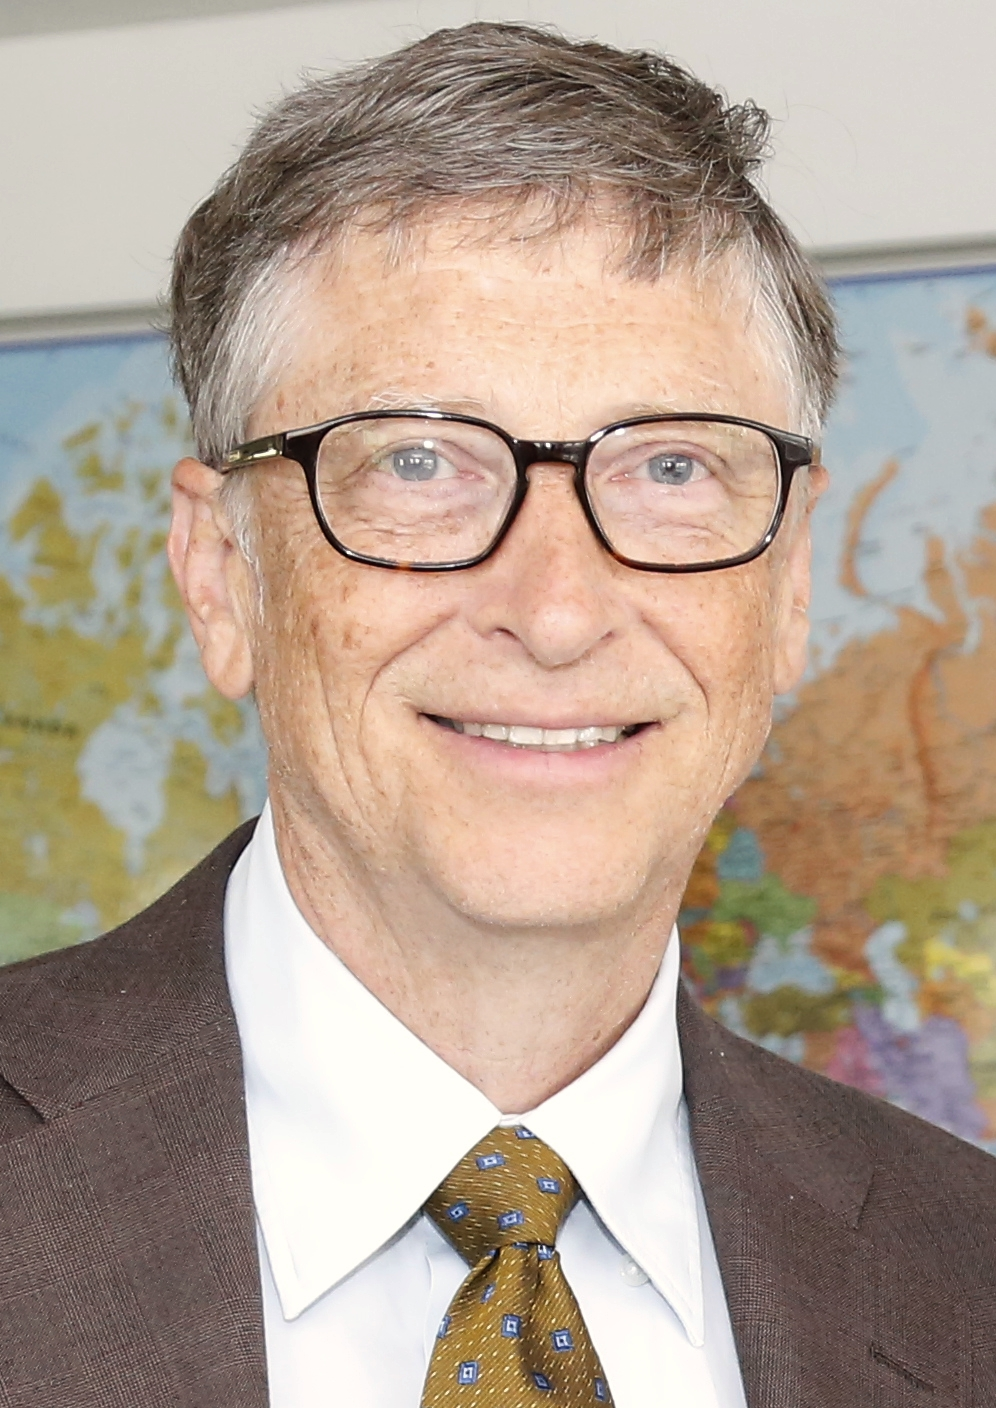
\includegraphics[width=1in]{img/Bill_Gates_June_2015}
%https://commons.wikimedia.org/wiki/File:Bill_Gates_June_2015.jpg
\end{minipage}
\end{center}

Bill Gates meant\footnote{This quote is on page 265 of the first
  edition.  In the second edition, on page 303, this sentence is
  changed to ``The obvious mathematical breakthrough that would defeat
  our public key encryption would be the development of an easy way to
  factor large numbers.''  This is less nonsensical; however, fast
  factoring is {\em not} known to break all commonly used public-key
  cryptosystem.  For example, there are cryptosystems based on the
  difficulty of computing discrete logarithms in $\FF_p^*$ and on
  elliptic curves over $\FF_p$, which (presumably) would not be broken
  even if one could factor large numbers quickly.}  factoring products
of two primes, which would break the RSA cryptosystem (see
e.g. \cite[\S3.2]{stein:ent}).  However, perhaps Gates is an
algebraic number theorist, and he really meant what he said: then we
might imagine that he meant factorization of primes of~$\ZZ$ in rings
of integers of number fields.  For example, $2^{16}+1 = 65537$ is a
``large'' prime, and in $\ZZ[i]$ we have
$$
  (65537) = (65537, 2^8 + i) \cdot (65537, 2^8 - i).
$$

\subsection{Geometric Intuition}\label{sec:geom_intuition}

\begin{figure}[ht!]
  \centering
  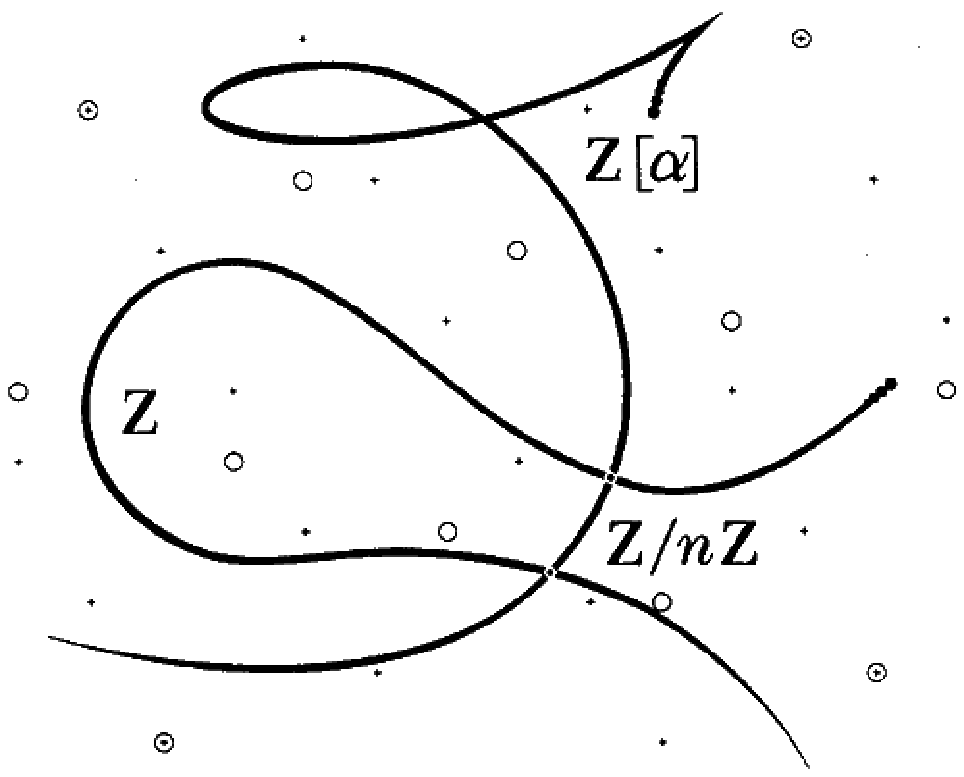
\includegraphics[width=20em]{img/spec}
  \caption{A diagram from the cover of \cite{lenstras:nfs}}.\label{fig:lenstra-cover}
\end{figure}

Let $K=\QQ(\alpha)$ be a number field, and let $\sO_K$ be the ring of integers
of $K$. To employ our geometric intuition, as the Lenstras did on the cover
of \cite{lenstras:nfs}
(see Figure~\ref{fig:lenstra-cover}),
it is helpful to view $\sO_K$ as a 1-dimensional scheme
$$
  X = \Spec(\sO_K) = \{\text{all prime ideals of $\sO_K$}\}
$$
over
$$
  Y=\Spec(\ZZ) = \{ (0) \} \cup \{ p\ZZ : p \in\ZZ_{>0} \text{ is prime}\}.
$$
There is a natural map $\pi: X \rightarrow Y$ that sends a prime ideal $\p\in X$ to
$\p \cap \ZZ\in Y$. For example, if
$$
  \p = (65537, 2^8 + i) \subset \ZZ[i],
$$
then $\p \cap \ZZ = (65537)$. For more on this viewpoint,
see \cite{hartshorne} and \cite[Ch.~2]{eisenbud_harris:geometry}.

If $p\in\ZZ$ is a prime number, then the ideal $p\sO_K$ of $\sO_K$
factors uniquely as a product $\prod \p_i^{e_i}$, where the $\p_i$ are
maximal ideals of $\sO_K$.  We may imagine the decomposition of $p\sO_K$
into prime ideals geometrically as the fiber $\pi^{-1}(p\ZZ)$, where
the exponents $e_i$ are the multiplicities of the fibers.  Notice that
the elements of $\pi^{-1}(p\ZZ)$ are the prime ideals of $\sO_K$ that
contain~$p$, i.e., the primes that divide $p\sO_K$.
This chapter is about how to compute the $\p_i$ and $e_i$.

\begin{remark}
  More technically, in algebraic geometry one defines the inverse
  image of the point $p\ZZ$ to be the spectrum of the tensor product
  $\sO_K \otimes_{\ZZ} \ZZ/\p\ZZ$; by a generalization of the Chinese
  Remainder Theorem, we have
  $$
    \sO_K \otimes_{\ZZ} \left(\ZZ/\p\ZZ\right) \isom \bigoplus \sO_K/\p_i^{e_i}.
  $$
\end{remark}

\begin{exercise}
  Let $L/K$ be an extension of number fields. Let $\p$ be a prime of $K$.
  Show that the factorization of the ideal $\p\sO_L$ contains exactly the primes
  of $\sO_L$ that lay over $\p$. That is, a prime $\q$ of $\sO_L$ appears in
  the factorization of $\p\sO_L$ if and only if $\q \cap \sO_K = \p$.
\end{exercise}

\begin{exercise}
  Let $\varphi: R \to S$ be a homomorphism of (commutative) rings.
  \begin{enumerate}[label=(\alph*)]
    \item Prove that if $I \subset S$ is an ideal, then $\varphi^{-1}(I)$
    is an ideal of~$R$.
    \item Prove moreover that if $I$ is prime, then $\varphi^{-1}(I)$ is
    also prime.
  \end{enumerate}
\end{exercise}

\begin{exercise}
  Let $\sO_K$ be the ring of integers of a number field.
  The \defn{Zariski topology} on the set $X=\Spec(\sO_K)$ of all prime ideals
  of $\sO_K$ has closed sets the sets of the form
  $$
    V(I) = \{ \p\in X : \p \mid I\},
  $$
  where~$I$ varies through {\em all} ideals of $\sO_K$, and $\p\mid I$ means
  that $I \subset \p$.
  \begin{enumerate}[label=(\alph*)]
    \item\label{exercise:zariski-part-1} Prove that the collection of closed
    sets of the form $V(I)$ is a topology on $X$.
    \item Let $Y$ be the subset of nonzero prime ideals of $\sO_K$, with the
    induced topology. Use unique factorization of ideals to prove that the
    closed subsets of~$Y$ are exactly the finite subsets of~$Y$ along with
    the set~$Y$.
    \item Prove that the conclusion of the first part is still true
    if $\sO_K$ is replaced by an order in $\sO_K$, i.e., a subring that
    has finite index in $\sO_K$ as a $\ZZ$-module.
  \end{enumerate}
\end{exercise}

\begin{exercise}
  Let $\sO_K$ be the ring of integers of a number field $K$, and let $p\in\ZZ$
  be a prime number. What is the cardinality of $\sO_K/(p)$ in terms of $p$
  and $[K:\QQ]$, where $(p)$ is the ideal of $\sO_K$ generated by~$p$?
\end{exercise}

\begin{exercise}
  Which of the following rings have infinitely many prime ideals?
  \begin{enumerate}[label=(\alph*)]
    \item
    The integers $\ZZ$.
    \item
    The ring $\ZZ[x]$ of polynomials over $\ZZ$.
    \item
    The quotient ring $\CC[x]/(x^{2005}-1)$.
    \item
    The ring $(\ZZ/6\ZZ)[x]$ of polynomials over the ring $\ZZ/6\ZZ$.
    \item
    The quotient ring $\ZZ/n\ZZ$, for a fixed positive integer~$n$.
    \item
    The rational numbers~$\QQ$.
    \item
    The polynomial ring $\QQ[x,y,z]$ in three variables.
  \end{enumerate}
\end{exercise}

\subsection{Examples}

The following {\Sage} session shows the commands needed to compute
the factorization of $p\sO_K$ for~$K$ the number field defined by
a root of $x^5 + 7x^4 + 3x^2 - x + 1$ and $p = 2$ and~$5$. We first
create an element $f\in \QQ[x]$ in {\Sage}:
\begin{sagecode}
\begin{sagecell}
R.<x> = QQ[]
f = x^5 + 7*x^4 + 3*x^2 - x + 1
\end{sagecell}
\end{sagecode} %link

\noindent
Then we create the corresponding number field obtained
by adjoining a root of $f$, and find its ring of integers.
\begin{sagecode} %link
\begin{sagecell}
K.<a> = NumberField(f)
OK = K.ring_of_integers()
OK.basis()
\end{sagecell}
\begin{sageout}
[1, a, a^2, a^3, a^4]
\end{sageout}
\end{sagecode} %link

\noindent
We define the ideal $2\sO_K$ and factor -- it turns out to be prime.

\begin{sagecode} %link
\begin{sagecell}
I = K.fractional_ideal(2); I
\end{sagecell}
\begin{sageout}
Fractional ideal (2)
\end{sageout}
\begin{sagecell}
I.factor()
\end{sagecell}
\begin{sageout}
Fractional ideal (2)
\end{sageout}
\begin{sagecell}
I.is_prime()
\end{sagecell}
\begin{sageout}
True
\end{sageout}
\end{sagecode} %link

\noindent
Finally we factor $5\sO_K$, which factors as a product of three primes.

\begin{sagecode} %link
\begin{sagecell}
I = K.fractional_ideal(5); I
\end{sagecell}
\begin{sageout}
Fractional ideal (5)
\end{sageout}
\begin{sagecell}
I.factor()
\end{sagecell}
\begin{sageout}
(Fractional ideal (5, -2*a^4 - 13*a^3 + 7*a^2 - 6*a + 2)) * \
(Fractional ideal (5, a^4 + 7*a^3 + 3*a + 1)) * \
(Fractional ideal (5, a^4 + 7*a^3 + 3*a - 3))^2
\end{sageout}
\end{sagecode} %link

\noindent
Notice that the polynomial $f$ factors in a similar way:

\begin{sagecode} %link
\begin{sagecell}
f.factor_mod(5)
\end{sagecell}
\begin{sageout}
(x + 2) * (x + 3)^2 * (x^2 + 4*x + 2)
\end{sageout}
\end{sagecode}
Thus $2\sO_K$ is already a prime ideal, and
$$
  5\sO_K = (5,2+a)\cdot(5,3+a)^2\cdot(5,2+4a+a^2).
$$
Notice that in this example $\sO_K=\ZZ[a]$. (Warning: There are examples of
$\sO_K$ such that $\sO_K\neq \ZZ[a]$ for any $a\in\sO_K$, as
Example~\ref{ex:dedekind} below illustrates.) When $\sO_K=\ZZ[a]$ it is
relatively easy to factor $p\sO_K$, at least assuming one can factor
polynomials in $\FF_p[x]$.
The following factorization gives a hint as to why:
$$
  x^5+7x^4+3x^2-x+1 \equiv (x+2) \cdot (x+3)^2 \cdot (x^2+4x+2)\pmod{5}.
$$

The exponent~$2$ of $(5,3+a)^2$ in the factorization of $5\sO_K$ above
suggests ``ramification'', in the sense that the cover $X \rightarrow Y$ has
less points (counting their ``size'', i.e., their residue class degree)
in its fiber over~$5$ than it has generically.
See Figure~\ref{fig:O_KoverSpecZ}.

\begin{figure}
\centering
$$
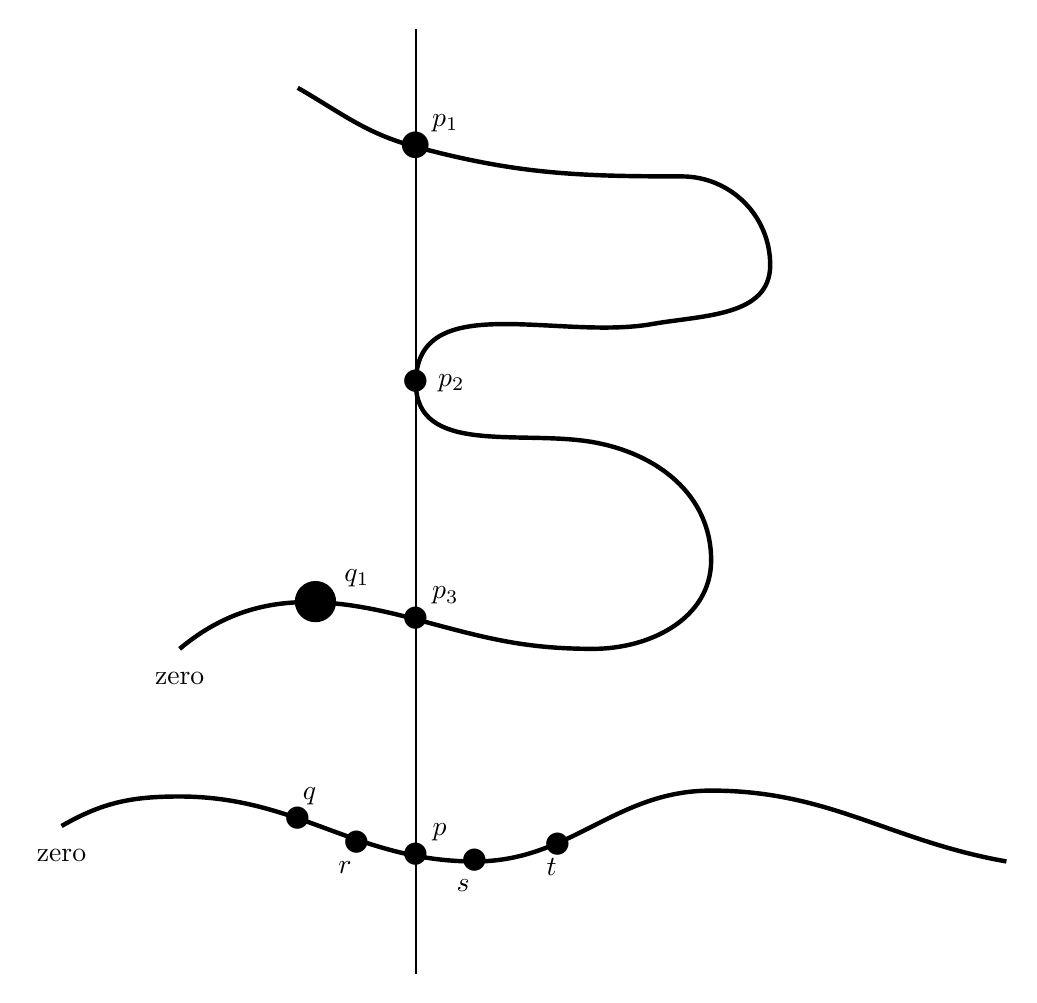
\begin{tikzpicture}[scale = 1.5]

\draw[thick] (0, 0) to (0, 8);

\node at (-3, 1) {zero};

\node at (0, 1) {\huge $\bullet$};
\node at (.2, 1.2) {$p$};

\node at (-1, 1.3) {\huge $\bullet$};
\node at (-.9, 1.5) {$q$};

\node at (-2, 2.5) {zero};

\draw [fill] (-.85, 3.15) circle [radius = .17];
\node at (-.5, 3.35) {$q_1$};

\node at (-.5, 1.1) {\huge $\bullet$};
\node at (-.6, .9) {$r$};

\node at (.5, .95) {\huge $\bullet$};
\node at (.4, .75) {$s$};

\node at (1.2, 1.08) {\huge $\bullet$};
\node at (1.15, .9) {$t$};

\node at (0, 3) {\huge $\bullet$};
\node at (.25, 3.2) {$p_3$};

\node at (0, 5) {\huge $\bullet$};
\node at (.3, 5) {$p_2$};

\node at (0, 7) {\Huge $\bullet$};
\node at (.25, 7.2) {$p_1$};

\draw[ultra thick] (-3, 1.25) to [out = 30, in = 180] (-2, 1.5) to [out = 0, in = 180] (.5, .95) to [out = 0, in = 180] (2.5, 1.55) to [out = 0, in = 170] (5, .95);

\draw[ultra thick] (-2, 2.75) to [out = 40, in = 165] (0, 3) to [out = -15, in = 180] (1.5, 2.75) to [out = 0, in = -90] (2.5, 3.5) to [out = 90, in = -10] (1.5, 4.5) to [out = 170, in = -90] (0, 5) to [out = 90, in = 190] (2, 5.5) to [out = 10, in = -90] (3, 6) to [out = 90, in = 0] (2.25, 6.75) to [out = 180, in = -15] (0, 7) to [out = 165, in = -30] (-1, 7.5);

\end{tikzpicture}
$$
\caption{Diagram of $\Spec(\sO_K) \rightarrow \Spec(\ZZ)$}
\label{fig:O_KoverSpecZ}
\end{figure}


\section{A Method for Factoring Primes that Often Works}

Suppose $a\in\sO_K$ is such that $K=\QQ(a)$, and let $f(x) \in \ZZ[x]$
be the minimal polynomial of~$a$. Then $\ZZ[a]\subset \sO_K$, and
we have a diagram of schemes
$$
  \begin{tikzcd}
    \displaystyle\bigcup\Spec\left(\sO_K/\p_i^{e_i}\right) \ar[r,hook] \ar[d] & \Spec(\sO_K) \ar[d]
    \\
    \displaystyle\bigcup\Spec\left(\FF_p[x]/(\overline{f}_i^{e_i})\right) \ar[r,hook] \ar[d] & \Spec(\ZZ[a]) \ar[d]
    \\
    \Spec(\FF_p) \ar[r,hook] & \Spec(\ZZ)
  \end{tikzcd}
$$

where $\overline{f} = \prod_i \overline{f}_i^{e_i}$ is the factorization of the
image of $f$ in $\FF_p[x]$, and $p\sO_K = \prod \p_i^{e_i}$ is the factorization
of $p\sO_K$ in terms of prime ideals of $\sO_K$. On the level of rings, the
bottom horizontal map is the quotient map $\ZZ\to\ZZ/p\ZZ\isom \FF_p$.
The middle horizontal map is induced by
$$
  \ZZ[x] \to \bigoplus_i \FF_p[x]/(\overline{f}_i^{e_i}),
$$
and the top horizontal map is induced by
$$
  \sO_K \to \sO_K/p\sO_K \isom \bigoplus \sO_K/\p_i^{e_i},
$$
where the isomorphism is by the Chinese Remainder Theorem,
which is Theorem~\ref{thm:crt} below.
The left vertical maps come from the inclusions
$$
   \FF_p \hookrightarrow \FF_p[x]/(\overline{f}_i^{e_i}) \hookrightarrow \sO_K/\p_i^{e_i},
$$
and the right from the inclusions $\ZZ \hookrightarrow \ZZ[a] \hookrightarrow \sO_K$.

The cover $\pi:\Spec(\ZZ[a]) \rightarrow \Spec(\ZZ)$ is easy to understand because it is
defined by the single equation $f(x)$,
in the sense that $\ZZ[a] \isom \ZZ[x]/(f(x))$.
To give a maximal ideal~$\p$ of $\ZZ[a]$ such that $\pi(\p) = p\ZZ$ is the same
as giving a homomorphism $\varphi: \ZZ[x]/(f) \rightarrow \overline{\FF}_p$ up to automorphisms of
the image, which is in turn the same as giving a root of~$f$ in $\overline{\FF}_p$ up
to automorphism, which is the same as giving an irreducible factor of the
reduction of~$f$ modulo~$p$.

\begin{lemma}\ilem{factorization of $p\sO_K$}\label{lem:factpok}
  Suppose the index of $\ZZ[a]$ in $\sO_K$ is coprime to~$p$.
  Then the primes~$\p_i$ in the factorization of $p\ZZ[a]$ do not
  decompose further going from $\ZZ[a]$ to $\sO_K$, so finding the
  prime ideals of $\ZZ[a]$ that contain~$p$ yields the primes
  that appear in the factorization of $p\sO_K$.
\end{lemma}
\begin{proof}
  % {\em Low-brow argument:}
  Fix a basis for $\sO_K$ and for $\ZZ[a]$ as $\ZZ$-modules.
  Form the matrix~$A$ whose columns express each basis element
  of $\ZZ[a]$ as a $\ZZ$-linear combination of the basis for $\sO_K$.
  Then
  $$
    \det(A) = \pm [\sO_K:\ZZ[a]]
  $$
  is coprime to~$p$, by hypothesis. Thus the reduction of~$A$
  modulo~$p$ is invertible, so it defines an isomorphism
  $\ZZ[a]/p\ZZ[a] \isom \sO_K/p\sO_K$.

  Let $\overline{\FF}_p$ denote a fixed algebraic closure of $\FF_p$; thus $\overline{\FF}_p$
  is an algebraically closed field of characteristic~$p$, over which
  all polynomials in $\FF_p[x]$ factor into linear factors.
  Any homomorphism $\sO_K\to \overline{\FF}_p$ sends~$p$ to~$0$, so is the composition
  of a homomorphism $\sO_K \to \sO_K/p\sO_K$ with a homomorphism
  $\sO_K/p\sO_K \to \overline{\FF}_p$. Since $\sO_K/p\sO_K \isom \ZZ[a]/p\ZZ[a]$, the
  homomorphisms $\sO_K\to \overline{\FF}_p$ are in bijection with the homomorphisms
  $\ZZ[a]\to \overline{\FF}_p$. The homomorphisms $\ZZ[a]\to\overline{\FF}_p$ are in bijection
  with the roots of the reduction modulo~$p$ of the minimal polynomial
  of~$a$ in $\overline{\FF}_p$.
\end{proof}

\begin{remark}
  Here is a ``high-brow'' proof of Lemma~\ref{lem:factpok}.
  By hypothesis we have an exact sequence of abelian groups
  $$
    0 \to \ZZ[a] \to \sO_K \to H \to 0,
  $$
  where $H$ is a finite abelian group of order coprime to~$p$.
  Tensor product is right exact, and there is an exact sequence
  $$
     \Tor_1(H,\FF_p) \to \ZZ[a]\otimes\FF_p \to \sO_K\otimes\FF_p \to H\otimes\FF_p \to 0,
  $$
  and $\Tor_1(H,\FF_p) = 0$ (since $H$ has no $p$-torsion),
  so $\ZZ[a]\otimes\FF_p \isom \sO_K\otimes\FF_p$.
\end{remark}

As suggested in the proof of the lemma, we find all homomorphisms
$\sO_K\to \overline{\FF}_p$ by finding all homomorphism
$\ZZ[a] \to \overline{\FF}_p$.  In
terms of ideals, if $\p = (f(a),p)\ZZ[a]$ is a maximal ideal of $\ZZ[a]$,
then the ideal $\p' = (f(a),p)\sO_K$ of $\sO_K$ is also maximal, since
$$
  \sO_K/\p'\isom (\sO_K/p\sO_K)/(f(\tilde{a}))
  \isom
  (\ZZ[a]/p\ZZ[a]) / (f(\tilde{a})) \subset \overline{\FF}_p,
$$
where $\tilde{a}$ denotes the image of $a$ in $\sO_K/p\sO_K$.

We formalize the above discussion, together with
Exercise~\ref{exercise:ramification-for-prime-factoring-easy-way} below,
in the following theorem:
\begin{theorem}\label{thm:fac1}\ithm{prime ideal factorization}
  Let $f\in\ZZ[x]$ be the minimal polynomial of~$a$ over~$\ZZ$.
  Suppose that~$p\nmid [\sO_K:\ZZ[a]]$ is a prime. Let
  $$
    \overline{f} = \prod_{i=1}^t \overline{f}_i^{e_i} \in \FF_p[x]
  $$
  where the $\overline{f}_i$ are distinct monic irreducible
  polynomials. Let $\p_i = (p,f_i(a))$ where $f_i\in\ZZ[x]$ is a
  lift of $\overline{f}_i$ in $\FF_p[x]$. Then
  $$
    p\sO_K = \prod_{i=1}^t \p_i^{e_i}.
  $$
  %Geometrically, the fiber of $\Spec(\sO_K) \to p\ZZ$
  %contains the points $\{\p_1,\p_2,\ldots, \p_t\}$
  %with multiplicites $e_i$.
\end{theorem}

\begin{exercise}\label{exercise:ramification-for-prime-factoring-easy-way}
  Let $p$ be a prime. Let $\sO_K$ be the ring of integers of a number
  field $K$, and suppose that $a\in \sO_K$ is such that $[\sO_K:\ZZ[a]]$ is
  finite and coprime to~$p$. Let $f(x)$ be the minimal polynomial of~$a$.
  We have already shows that if the reduction $\overline{f}\in\FF_p[x]$ of $f$
  factors as
  $$
    \overline{f} = \prod g_i^{e_i},
  $$
  where the $g_i$ are distinct irreducible polynomials in $\FF_p[x]$,
  then the primes appearing in the factorization of $p\sO_K$ are the
  ideals $(p,g_i(a))$. Show that the exponents of the primes in the
  factorization of $p\sO_K$ are the $e_i$.
\end{exercise}


We return to the example from above, in which $K = \QQ(a)$, where~$a$ is
a root of $f = x^5 + 7x^4 + 3x^2 - x + 1$.  The ring of integers~$\sO_K$
has discriminant $2945785 = 5\cdot 353\cdot 1669$, as the following
{\Sage} code shows.
\begin{sagecode}
\begin{sagecell}
K.<a> = NumberField(x^5 + 7*x^4 + 3*x^2 - x + 1)
D = K.discriminant(); D
\end{sagecell}
\begin{sageout}
2945785
\end{sageout}
\begin{sagecell}
factor(D)
\end{sagecell}
\begin{sageout}
5 * 353 * 1669
\end{sageout}
\end{sagecode}
The order $\ZZ[a]$ has the same discriminant as $f(x)$, which
is the same as the discriminant of $\sO_K$, so
$\ZZ[a] = \sO_K$ and we can apply the above theorem.
(Here we use that the index of $\ZZ[a]$ in $\sO_K$
is the square of the quotient of their discriminants,
a fact we will prove later in Section~\ref{sec:disc}.)
\begin{sagecode}
\begin{sagecell}
R.<x> = QQ[]
discriminant(x^5 + 7*x^4 + 3*x^2 - x + 1)
\end{sagecell}
\begin{sageout}
2945785
\end{sageout}
\end{sagecode}
We have
$$
  x^5+7x^4+3x^2-x+1 \equiv (x+2) \cdot (x+3)^2 \cdot (x^2+4x+2)\pmod{5},
$$
which yields the factorization of $5\sO_K$ given before the theorem.

If we replace $a$ by $b = 7a$, then the index of $\ZZ[b]$
in $\sO_K$ will be a power of $7$, which is coprime to $5$,
so the above method will still work.
\begin{sagecode}
\begin{sagecell}
K.<a> = NumberField(x^5 + 7*x^4 + 3*x^2 - x + 1)
f = (7*a).minpoly('x')
f
\end{sagecell}
\begin{sageout}
x^5 + 49*x^4 + 1029*x^2 - 2401*x + 16807
\end{sageout}
\begin{sagecell}
f.disc()
\end{sagecell}
\begin{sageout}
235050861175510968365785
\end{sageout}
\begin{sagecell}
factor(f.disc() / K.disc())
\end{sagecell}
\begin{sageout}
7^20
\end{sageout}
\begin{sagecell}
f.factor_mod(5)
\end{sagecell}
\begin{sageout}
(x + 4) * (x + 1)^2 * (x^2 + 3*x + 3)
\end{sageout}
\end{sagecode}
Thus $5$ factors in $\sO_K$
as
$$
  5\sO_K = (5, 7a+1)^2 \cdot (5, 7a+4) \cdot (5, (7a)^2 + 3(7a) + 3).
$$
If we replace $a$ by $b=5a$ and try the above algorithm with $\ZZ[b]$, then
the method fails because the index of $\ZZ[b]$ in $\sO_K$ is divisible by~$5$.
\begin{sagecode}
\begin{sagecell}
K.<a> = NumberField(x^5 + 7*x^4 + 3*x^2 - x + 1)
f = (5*a).minpoly('x')
f
\end{sagecell}
\begin{sageout}
x^5 + 35*x^4 + 375*x^2 - 625*x + 3125
\end{sageout}
\begin{sagecell}
f.factor_mod(5)
\end{sagecell}
\begin{sageout}
x^5
\end{sageout}
\end{sagecode}

\section{A General Method}

There are numbers fields $K$ such that $\sO_K$ is not of the form
$\ZZ[a]$ for any $a\in K$.  Even worse, Dedekind found a
field~$K$ such that $2\mid [\sO_K : \ZZ[a]]$ for {\em all}
$a\in \sO_K$, so there is no choice of $a$ such that Theorem~\ref{thm:fac1}
can be used to factor~$2$ for $K$ (see Example~\ref{ex:dedekind} below).

\subsection{Inessential Discriminant Divisors}

\begin{definition}
  A prime $p$ is an \defn{inessential discriminant divisor}
  if $p\mid [\sO_K : \ZZ[a]]$ for {\em every} $a\in\sO_K$.
\end{definition}
See Example~\ref{ex:exdim} below for why it is called an
inessential ``discriminant divisor'' instead of an
inessential ``index divisor''.

Since $[\sO_K : \ZZ[a]]^2$ is the absolute value of
$\Disc(f(x))/\Disc(\sO_K)$, where $f(x)$ is the characteristic
polynomial of $f(x)$, an inessential discriminant divisor divides the
discriminant of the characteristic polynomial of any element of
$\sO_K$.

\begin{example}[Dedekind]\label{ex:dedekind}
  Let $K=\QQ(a)$ be the cubic field defined by a root $a$ of the polynomial
  $f = x^3 + x^2 - 2x+8$.  We will use {\Sage} to show that~$2$ is an
  inessential discriminant divisor for~$K$.
\begin{sagecode}
\begin{sagecell}
K.<a> = NumberField(x^3 + x^2 - 2*x + 8); K
\end{sagecell}
\begin{sageout}
Number Field in a with defining polynomial x^3 + x^2 - 2*x + 8
\end{sageout}
\begin{sagecell}
K.factor(2)
\end{sagecell}
\begin{sageout}
(Fractional ideal (1/2*a^2 - 1/2*a + 1)) * \
(Fractional ideal (-a^2 + 2*a - 3)) * \
(Fractional ideal (-3/2*a^2 + 5/2*a - 4))
\end{sageout}
\end{sagecode}
  Thus $2\sO_K = \p_1\p_2\p_3$, with the $\p_i$ distinct,
  and one sees directly from the above expressions
  that $\sO_K/\p_i \isom \FF_2$ for each $i$. If $\sO_K = \ZZ[a]$
  for some $a \in \sO_K$ with minimal polynomial~$f$, then
  $\overline{f}(x) \in \FF_2[x]$ must be a product of three {\em distinct}
  linear factors, which is impossible, since the only
  linear polynomials in $\FF_2[x]$ are $x$ and $x+1$.
\end{example}

\begin{exercise}
  Find an example of a field $K$ of degree at least~$4$ such that the ring
  $\sO_K$ of integers of $K$ is not of the form $\ZZ[a]$ for any $a\in \sO_K$.
\end{exercise}

\begin{exercise}
  Let $\p$ be a prime ideal of $\sO_K$, and suppose that $\sO_K/\p$
  is a finite field of characteristic $p\in\ZZ$.  Prove that there is
  an element $\alpha\in\sO_K$ such that $\p=(p,\alpha)$.  This
  justifies why we can represent prime ideals of $\sO_K$ as pairs
  $(p,\alpha)$, as is done in {\Sage}. (More generally, if $I$ is an
  ideal of $\sO_K$, we can choose one of the elements of $I$ to be {\em
  any} nonzero element of $I$.)
\end{exercise}

\begin{exercise}
  Give an example of an order $\sO$ in the ring of integers of
  a number field and an ideal $I$ such that~$I$ cannot be generated by
  $2$ elements as an ideal.

  \begin{hint}
    This problem is more difficult than usual.
  \end{hint}
\end{exercise}

\subsection{Remarks on Ideal Factorization in General}

Recall (from Definition~\ref{defn:order}) that an {\em order} in $\sO_K$ is
a subring $\sO$ of $\sO_K$ that has finite index in $\sO_K$.  For
example, if $\sO_K = \ZZ[i]$, then $\sO = \ZZ + 5\ZZ[i]$ is an order in $\sO_K$,
and as an abelian group $\sO_K/\sO$ is cyclic of order~$5$.

Most algebraic number theory books do not describe an algorithm for
decomposing primes in the general case.  Fortunately, Cohen's book
\cite[Ch.~6]{cohen:course_ant} does describe how to solve the general
problem, in more than one way.  The algorithms are nontrivial, and
occupy a substantial part of Chapter~6 of Cohen's book.  Our goal
for the rest of this section is to give a hint as to what goes into them.

The general solutions to prime ideal factorization are somewhat surprising,
since the algorithms are much more sophisticated than the one
suggested by Theorem~\ref{thm:fac1}.  However, these complicated
algorithms all run very quickly in practice, even without assuming the
maximal order is already known.  In fact, they avoid computing~$\sO_K$
altogether, and instead compute only an order~$\sO$ that is {\em $p$-maximal},
i.e., is such that $p \nmid [\sO_K:\sO]$.

For simplicity we consider the following slightly easier problem whose
solution illustrates the key ideas needed in the general case.
\begin{problem}\label{prob:pcontained}
  Let $\sO$ be any order in $\sO_K$ and let~$p$ be a prime of $\ZZ$.
  Find the prime ideals of $\sO$ that contain~$p$.
\end{problem}

Given a prime~$p$
that we wish to factor in $\sO_K$, we first find a $p$-maximal order~$\sO$.
We then use a solution to Problem~\ref{prob:pcontained} to find
the prime ideals $\p$ of $\sO$ that contain $p$.  Second, we find
the exponents $e$ such that $\p^e$ exactly divides $p\sO$.
The resulting factorization in $\sO$ completely determines
the factorization of $p\sO_K$.

A $p$-maximal order can be found reasonably quickly in practice using
algorithms called ``round 2'' and ``round 4''.  To
compute $\sO_K$, given an order $\ZZ[\alpha]\subset \sO_K$, one takes a
sum of $p$-maximal orders, one for every~$p$ such that $p^2$ divides
$\Disc(\ZZ[\alpha])$.  The time-consuming part of this computation is
finding the primes~$p$ such that $p^2\mid \Disc(\ZZ[\alpha])$, not
finding the $p$-maximal orders.  This example illustrates that
a fast algorithm for factoring integers would not only break the RSA
cryptosystems, but would massively speed up computation of the ring of
integers of a number field.
\begin{remark}
  The MathSciNet review of \cite{buchmann_lenstra:approx} by
  J.~Buhler contains the following:
  \begin{quote}
      A result of Chistov says that finding the ring of integers $\sO_K$
      in an algebraic number field $K$ is equivalent, under certain
      polynomial time reductions, to the problem of finding the largest
      squarefree divisor of a positive integer. No feasible (i.e.,
      polynomial time) algorithm is known for the latter problem, and it
      is possible that it is no easier than the more general problem of
      factoring integers.
  \end{quote}
  Thus it appears that computing the ring $\sO_K$ is quite hard.
\end{remark}

\subsection{Finding a $p$-Maximal Order}\label{sec:alg_pmax}

Before describing the general factorization algorithm, we sketch some
of the theory behind the general algorithms for computing a
$p$-maximal order $\sO$ in $\sO_K$.  The main input is the following theorem:
\begin{theorem}[Pohst-Zassenhaus]
  Let $\sO$ be an order in the ring of integers $\sO_K$ of a number field,
  let $p\in\ZZ$ be a prime, and let
  $$
    I_p = \{x \in \sO : x^m \in p\sO \text{ for some $m\geq 1$}\} \subset \sO
  $$
  be the radical of $p\sO$, which is an ideal of $\sO$. Let
  $$
    \sO' = \{x \in K : xI_p \subset I_p\}.
  $$
  Then $\sO'$ is an order and either $\sO'=\sO$, in which case $\sO$ is
  $p$-maximal, or $\sO\subset\sO'$ and $p$ divides $[\sO':\sO]$.
\end{theorem}
\begin{proof}
  We prove here only that $[\sO':\sO] \mid p^n$, where $n$ is the degree
  of $K$.  We have $p\in I_p$, so if $x \in \sO'$, then $xp \in
  I_p\subset \sO$, which implies that $x\in \frac{1}{p}\sO$.  Since
  $(\frac{1}{p}\sO)/\sO$ is of order $p^n$, the claim follows.

  To complete the proof, we would show that if $\sO' = \sO$, then $\sO$ is
  already $p$-maximal.  See \cite[\S6.1.1]{cohen:course_ant} for the
  rest if this proof.
\end{proof}

After deciding on how to represent elements of~$K$ and orders and
ideals in~$K$, one can give an efficient algorithm to compute the
$\sO'$ of the theorem.  The algorithm mainly involves linear algebra
over finite fields.  It is complicated to describe, but efficient in
practice, and is conceptually simple---just compute~$\sO'$.  The trick
for reducing the computation of $\sO'$ to linear algebra is the
following lemma:
\begin{lemma}
  Define a homomorphism $\psi:\sO \hookrightarrow \End(I_p/ p I_p)$ given by
  sending $\alpha\in\sO$ to left multiplication by the reduction of
  $\alpha$ modulo~$p$.  Then
  $$
    \sO'=\frac{1}{p} \ker(\psi).
  $$
\end{lemma}
\begin{proof}
  If $x \in \sO'$, then $x I_p \subset I_P$, so $\psi(x)$ is the $0$
  endomorphism.  Conversely, if $\psi(x)$ acts as $0$ on $I_p/ p I_p$,
  then clearly $x I_p \subset I_p$.
\end{proof}

Note that to give an algorithm one must also figure out how to
explicitly compute $I_p/ p I_p$ and the kernel of this map
(see  the next section for more
details).

\subsection{General Factorization Algorithm of Buchman-Lenstra}

We finally give an algorithm to factor $p\sO_K$ in general. This is a
summary of the algorithm described in more detail in
\cite[\S6.2]{cohen:course_ant}.

\begin{algorithm}[Factoring a Finite Separable Algebra]\label{alg:factorsep}
  Let $A$ be a finite separable algebra over $\FF_p$.  This
  algorithm either shows that $A$ is a field or finds
  a nontrivial idempotent in $A$, i.e., an $\varepsilon\in A$
  such that $\varepsilon^2 = \varepsilon$ with $\varepsilon\neq 0$ and $\varepsilon\neq 1$.
  \begin{enumerate}
    \item The dimension of the kernel $V$ of the map $x\mapsto x^p - x$ is
    equal to $k$.  This is because abstractly we have that $A\ncisom
    A_1\times \cdots \times A_k$, with each $A_i$ a finite field
    extension of $\FF_p$.
    \item If $k=1$ we are done.  Terminate.
    \item Otherwise, choose $\alpha \in V$ with $\alpha \not\in \FF_p$.
    (Think of $\FF_p$ as the diagonal embedding of $\FF_p$ in
    $A_1\times \cdots \times A_k$).
    Compute powers of $\alpha$ and find the minimal polynomial $m(X)$
    of $\alpha$.
    \item Since $V\ncisom \FF_p \times \cdots \times F_p$ ($k$ factors),
    the polynomial $m(X)$ is a square-free product of linear factors, that
    has degree $>1$ since $\alpha\not\in\FF_p$.  Thus we can compute
    a splitting $m(X) = m_1(X) \cdot m_2(X)$, where both $m_i(X)$ have
    positive degree.
    \item Use the Euclidean algorithm in $\FF_p[X]$ to find
    $U_1(X)$ and $U_2(X)$ such that
    $$
      U_1 m_1 + U_2 m_2 = 1.
    $$
    \item Let $\varepsilon = (U_1 m_1)(\alpha)$.  Then we have
    $$
      U_1 m_1 U_1 m_1 + U_2 m_2 U_1 m_1 = U_1 m_1,
    $$
    so since $(m_1 m_2)(\alpha) = m(\alpha)=01$, we have $\varepsilon^2 = \varepsilon$.
    Also, since $\gcd(U_1, m_2) = \gcd(U_2, m_1) = 1$,
    we have $\varepsilon\neq 0$ and $\varepsilon \neq 1$.
  \end{enumerate}
\end{algorithm}

Given Algorithm~\ref{alg:factorsep}, we compute an idempotent
$\varepsilon \in A$, and observe that
$$
  A \isom \ker(1 - \varepsilon)  \oplus \ker(\varepsilon).
$$
Since $(1 - \varepsilon) + \varepsilon = 1$, we see that
$(1 - \varepsilon)v + \varepsilon v = v$, so that the sum
of the two kernels equals $A$.
Also, if $v$ is in the intersection of the two kernels,
then $\varepsilon(v) = 0$ and $(1-\varepsilon)(v) =0$, so
$0 = (1-\varepsilon)(v) = v - \varepsilon(v) = v$, so the sum is direct.

\begin{remark}
  The beginning of \cite[\S6.2.4]{cohen:course_ant} suggests that one
  can just randomly find an $\alpha \in A$ such that $A\isom
  \FF_p[x]/(m(x))$ where $m$ is the minimal polynomial of $\alpha$.
  This is usually the case, but is {\em wrong in general}, since there
  need {\em not} be an $\alpha \in A$ such that $A \isom
  \FF_p[\alpha]$.  For example, let $p=2$ and $K$ be as in
  Example~\ref{ex:dedekind}.  Then $A \isom \FF_2 \times \FF_2 \times
  \FF_2$, which as a ring is not generated by a single element, since
  there are only 2 distinct linear polynomials over $\FF_2[x]$.
\end{remark}

\begin{algorithm}[Factoring a General Prime Ideal]\label{alg:genfac}
  Let $K=\QQ(a)$ be a number field given by an algebraic integer~$a$
  as a root of its minimal monic polynomial~$f$ of degree~$n$.
  We assume that an order $\sO$ has been given by a basis $w_1,\ldots,w_n$
  and that~$\sO$ that contains $\ZZ[a]$.
  For any prime $p\in\ZZ$, the following algorithm computes the set of
  maximal ideals of~$\sO$ that contain~$p$.
  \begin{description}
    \item[\normalfont (Check if easy):] If $p \nmid \Disc(\ZZ[a]) / \Disc(\sO)$ (so
    $p \nmid [\sO:\ZZ[a]]$), then using Theorem~\ref{thm:fac1} we
    factor~$p\sO$.

    \item[\normalfont (Compute radical):]
    Let $I$ be the \defn{radical} of $p\sO$, which is the ideal of
    elements $x\in\sO$ such that $x^m\in p\sO$
    for some positive integer~$m$.  Note that $p\sO \subset I$, i.e.,
    $I\mid p\sO$; also~$I$ is the product
    of the primes that divide $p$, without multiplicity.
    Using linear algebra over the finite field
    $\FF_p$, we compute a basis for $I/p\sO$ by computing
    the abelian subgroup of $\sO/p\sO$ of all nilpotent
    elements.  This computes $I$, since $p\sO\subset I$.

    \item[\normalfont (Compute quotient by radical):]
    Compute an $\FF_p$ basis for
    $$
      A = \sO/I = (\sO/p\sO)/(I/p\sO).
    $$
    The second equality comes from the fact that $p\sO\subset I$.
    Note that $\sO/p\sO$
    is obtained by simply reducing the basis $w_1,\ldots, w_n$ modulo~$p$.
    Thus this step entirely involves linear algebra modulo $p$.

    \item[\normalfont (Decompose quotient):] The ring $A$ is isomorphic to
    the quotient of $\sO$ by a radical ideal,
    so it decomposes as a product
    $A \isom A_1 \times \cdots \times A_k$ of finite fields.
    We find such a decomposition explicitly using Algorithm~\ref{alg:factorsep}.

    \item[\normalfont (Compute the maximal ideals over $p$):] Each maximal ideal
    $\p_i$ lying over~$p$ is the kernel of one of the compositions
    $$
      \sO \to A \ncisom A_1 \times \cdots \times A_k \to A_i.
    $$
  \end{description}
\end{algorithm}
Algorithm~\ref{alg:genfac} finds all primes of $\sO$ that contain the radical $I$ of
$p\sO$.  Every such prime clearly contains $p$, so to see that the
algorithm is correct, we prove that the primes $\p$ of $\sO$ that
contain~$p$ also contain~$I$.  If $\p$ is a prime of $\sO$ that
contains~$p$, then $p\sO \subset \p$.  If $x\in I$ then $x^m\in p\sO$
for some $m$, so $x^m\in \p$ which implies that $x\in \p$ by the primality
of $\p$.  Thus $\p$ contains $I$, as required.  Note that we do not find the powers of
primes that divide $p$ in Algorithm~\ref{alg:genfac}; that's left to another
algorithm that we will not discuss in this book.

Algorithm~\ref{alg:genfac} was invented by J.~Buchmann and
H.W. Lenstra, though their paper seems to have never been
published; however, the algorithm is described in detail in
\cite[\S6.2.5]{cohen:course_ant}.  Incidentally, this chapter is based
on Chapters~4 and~6 of \cite{cohen:course_ant}, which is highly
recommended, and goes into much more detail about these algorithms.

\begin{exercise}
  Explicitly factor the ideals generated by each of $2$, $3$, and $5$ in
  the ring of integers of $\QQ(\sqrt[3]{2})$ (so you will factor $3$
  separate ideals as products of prime ideals.)
  You may assume that the ring of integers of $\QQ(\sqrt[3]{2})$
  is $\ZZ[\sqrt[3]{2}]$, but do \em{not} simply use a computer command to do
  the factorizations.
\end{exercise}

\begin{exercise}
  Let $K=\QQ(\zeta_{13})$,where $\zeta_{13}$ is a primitive $13$th root of
  unity. Note that~$K$ has ring of integers $\sO_K=\ZZ[\zeta_{13}]$.
  \begin{enumerate}[label=(\alph*)]
    \item Factor $2$, $3$, $5$, $7$, $11$, and $13$ in the ring
    of integers $\sO_K$.  You may use a computer.
    \item For $p\neq 13$, find a conjectural
    relationship between the number of prime ideal factors of $p\sO_K$
    and the order of the reduction of~$p$  in $(\ZZ/13\ZZ)^*$.
    \item Compute the minimal polynomial $f(x)\in\ZZ[x]$ of $\zeta_{13}$.
    Reinterpret your conjecture as a conjecture that
    relates the degrees of the irreducible factors of $f(x)\pmod{p}$ to
    the order of $p$ modulo~$13$. Does your conjecture
    remind you of quadratic reciprocity?
  \end{enumerate}
\end{exercise}

%%[[Add discussion about how to compute a $p$-maximal order here.]]
 %  factoring
%%%%%%%%%%%%%%%%%%%%%%%%%%%%%%%%%%%%%%%%%%%%%%%%%%%%%%%%%%%%%%%%%%%%%%%%%%%
%% CRT
%%%%%%%%%%%%%%%%%%%%%%%%%%%%%%%%%%%%%%%%%%%%%%%%%%%%%%%%%%%%%%%%%%%%%%%%%%

\chapter{The Chinese Remainder Theorem}\label{ch:crt}

In this chapter, we prove the Chinese Remainder Theorem (CRT) for
arbitrary commutative rings, then apply CRT to prove that every ideal
in a Dedekind domain $R$ is generated by at most two elements.  We
also prove that $\p^n/\p^{n+1}$ is (noncanonically) isomorphic to
$R/\p$ as an $R$-module, for any nonzero prime ideal $\p$ of $R$.  The
tools we develop in this chapter will be used frequently to prove
other results later.

\section{The Chinese Remainder Theorem}

\subsection{CRT in the Integers}
The classical CRT asserts that if $n_1, \dots, n_r$ are integers that are coprime
in pairs, and $a_1, \dots, a_r$ are integers, then there exists an
integer~$a$ such that $a \equiv a_i\pmod{n_i}$ for each $i=1, \dots,r$.
Here ``coprime in pairs'' means that $\gcd(n_i,n_j)=1$ whenever
$i\neq j$; it does {\em not} mean that $\gcd(n_1, \dots, n_r)=1$,
though it implies this.
In terms of rings, CRT asserts that the
natural map
\begin{equation}\label{eqn:crt}
\ZZ/(n_1\cdots n_r)\ZZ \to (\ZZ/n_1\ZZ)\oplus \cdots \oplus (\ZZ/n_r\ZZ)
\end{equation}
that sends $a \in \ZZ$ to its reduction modulo each $n_i$,
is an isomorphism.

This map is {\em never} an isomorphism if the $n_i$ are not coprime.
Indeed, the cardinality of the image of the left hand side of
(\ref{eqn:crt}) is $\lcm(n_1, \dots, n_r)$, since it is the image of a
cyclic group and $\lcm(n_1, \dots, n_r)$ is the largest order of an
element of the right hand side, whereas the cardinality of the right
hand side is $n_1\cdots n_r$.

The isomorphism (\ref{eqn:crt}) can alternatively be viewed as
asserting that any system of linear congruences
$$
x \equiv a_1 \pmod{n_1}, \quad
x \equiv a_2 \pmod{n_2}, \quad
\dots, \quad
x \equiv a_r \pmod{n_r}
$$
with pairwise coprime moduli has a unique solution modulo $n_1\cdots n_r$.

Before proving the CRT in more generality, we prove
(\ref{eqn:crt}).
There is a natural map
$$
  \phi: \ZZ \to (\ZZ/n_1\ZZ)\oplus \cdots \oplus (\ZZ/n_r\ZZ)
$$
given by projection onto each factor.  Its kernel is
$$
 n_1 \ZZ \cap \cdots \cap n_r \ZZ.
$$
If $n$ and $m$ are integers, then $n\ZZ\cap m\ZZ$ is the
set of multiples of both $n$ and $m$, so $n\ZZ\cap m\ZZ = \lcm(n,m)\ZZ$.
Since the $n_i$ are coprime,
$$
 n_1 \ZZ \cap \cdots \cap n_r \ZZ = n_1 \cdots n_r \ZZ.
$$
Thus we have proved there is an inclusion
\begin{equation}\label{eqn:crt_inj}
 i: \ZZ/(n_1\cdots n_r)\ZZ \hookrightarrow (\ZZ/n_1\ZZ) \oplus \cdots \oplus (\ZZ/n_r\ZZ).
\end{equation}
This is half of the CRT; the other half is to prove that this map is
surjective.  In this case, it is clear that $i$ is also surjective,
because $i$ is an injective map between finite sets of the same cardinality.
We will, however, give a proof of surjectivity that doesn't use
finiteness of the above two sets.

To prove surjectivity of $i$, note that since the $n_i$ are coprime in
pairs, $$\gcd(n_1, n_2\cdots n_r)=1,$$ so there exists integers $x,y$
such that
$$
   x n_1 + y n_2\cdots n_r = 1.
$$
To complete the proof, observe that
$ y n_2\cdots n_r = 1 - x n_1$
is congruent to~$1$ modulo $n_1$ and~$0$ modulo $n_2\cdots n_r$.
Thus $(1,0, \dots,0) = i (y n_2\cdots n_r)$ is in the image of~$i$.
By a similar argument, we see that $(0,1, \dots,0)$ and the
other similar elements are all in the image of~$i$, so $i$
is surjective, which proves CRT.

\subsection{CRT in General}
Recall that {\em all rings in this book are commutative with unity}.
Let $R$ be such a ring.

\begin{definition}[Coprime]
  Ideals $I$ and $J$ of $R$ are \defn{coprime} if $I+J=(1)$.
\end{definition}

\begin{exercise}
  Let $a_1 = 1+i$, $a_2 = 3+2i$, and $a_3 = 3+4i$ as elements of $\ZZ[i]$.
  \begin{enumerate}[label=(\alph*)]
    \item Prove that the ideals $I_1=(a_1)$, $I_2=(a_2)$, and $I_3=(a_3)$
    are coprime in pairs.
    \item Compute the cardinality of $\ZZ[i]/(I_1 I_2 I_3)$.
    \item Find a single element in $\ZZ[i]$ that is congruent to~$n$
    modulo $I_n$, for each $n\leq 3$.
  \end{enumerate}
\end{exercise}

For example, if~$I$ and~$J$ are nonzero ideals in a Dedekind domain,
then they are coprime precisely when the prime ideals that appear in
their two (unique) factorizations are disjoint.

\begin{lemma}\label{lem:prodint}\ilem{$I\cap{}J = IJ$}
If $I$ and $J$ are coprime ideals in a ring $R$, then
$I\cap{}J = IJ$.
\end{lemma}
\begin{proof}
Choose $x\in I$ and $y\in J$
such that $x+y=1$.  If $c\in{} I\cap{} J$ then
$$c=c\cdot 1=c\cdot (x+y) = cx + cy \in IJ + IJ = IJ,$$
so $I\cap{} J\subset IJ$.
The other inclusion is obvious by the definition of an ideal.
\end{proof}

\begin{lemma}\label{lem:coprime_prod}
Suppose $I_1, \dots, I_s$ are pairwise coprime ideals.
Then $I_1$ is coprime to the product $I_2\cdots I_s$.
\end{lemma}
\begin{proof}
In the special case of a Dedekind domain, we could easily
prove this lemma using unique factorization of ideals as
products of primes (Theorem~\ref{thm:intuniqfac}); instead,
we give a direct general argument.

It suffices to prove the lemma in the case $s=3$, since the
general case then follows from induction.
By assumption, there
are $x_1 \in I_1, y_2 \in I_2$ and $a_1 \in I_1, b_3 \in I_3$
such
$$
x_1 + y_2 = 1 \qquad\text{and}\qquad a_1 + b_3 = 1.
$$
Multiplying these two relations yields
$$
x_1 a_1 + x_1 b_3 + y_2 a_1 + y_2 b_3 = 1 \cdot 1 = 1.
$$
The first three terms are in $I_1$ and the last term is in
$I_2 I_3 = I_2 \cap I_3$ (by Lemma~\ref{lem:prodint}),
so $I_1$ is coprime to $I_2 I_3$.
\end{proof}

Next we prove the general Chinese Remainder Theorem.
We will apply this result with $R=\sO_K$ in the rest of this chapter.
\begin{theorem}[Chinese Remainder Theorem]\label{thm:crt}
\ithm{chinese remainder}
Suppose $I_1, \dots, I_r$ are nonzero ideals of a ring~$R$ such
$I_m$ and $I_n$ are coprime for any $m\neq n$.  Then the natural
homomorphism $R \to \bigoplus_{n=1}^r R/I_n$ induces an isomorphism
$$
\psi: R/\prod_{n=1}^r I_n \to \bigoplus_{n=1}^r R/I_n.
$$
Thus given any $a_n \in R$, for $n=1, \dots,r$, there exists some $a\in R$
such that $a \equiv a_n\pmod{I_n}$ for $n=1, \dots, r$; moreover,~$a$
is unique modulo $\prod_{n=1}^r I_n$.
\end{theorem}

\begin{proof}
Let
$
  \varphi:R \to \bigoplus_{n=1}^r R/I_n
$
be the natural map induced by reduction modulo
the $I_n$.
An inductive application of Lemma~\ref{lem:prodint}
implies that
the kernel $\cap_{n=1}^r I_n$ of~$\varphi$
is equal to
$\prod_{n=1}^r I_n$, so the map~$\psi$ of the theorem is injective.

Each projection $R\to R/I_n$ is  surjective, so to prove
that $\psi$ is surjective, it suffices
to show that $(1,0, \dots,0)$
is in the image of~$\varphi$, and similarly for the other
factors.  By Lemma~\ref{lem:coprime_prod},
$J=\prod_{n=2}^rI_n$ is coprime to~$I_1$, so
there exists $x\in I_1$ and $y \in J$ such that
$x+y=1$.  Then $y = 1-x$ maps to~$1$ in
$R/I_1$ and to~$0$ in $R/J$, hence to~$0$ in $R/I_n$
for each $n\geq 2$, since $J\subset I_n$.
\end{proof}

\section{Structural Applications of the CRT}
Let $\sO_K$ be the ring of integers of some number field $K$, and
suppose~$I$ is a nonzero ideal of $\sO_K$.  As an abelian group $\sO_K$
is free of rank $[K:\QQ]$, and~$I$ is of finite index in $\sO_K$, so~$I$
is generated by $[K:\QQ]$ generators as an abelian group, so as an
$R$-ideal $I$ requires at most $[K:\QQ]$ generators.  The main result
of this section asserts something better, namely that~$I$ can be
generated {\em as an ideal} by at most two elements.  Moreover, our
result is more general, since it applies to an arbitrary Dedekind
domain $R$. Thus, for the rest of this section, $R$ is any Dedekind
domain, e.g., the ring of integers of either a number field or
function field.  We use CRT to prove that every ideal of $R$ can be
generated by two elements.

\begin{warning}
If we replace $R$ by an order in a Dedekind domain, i.e.,
by a subring of finite index, then there may be ideals that
require far more than $2$ generators.
\end{warning}

Suppose that~$I$ is a nonzero integral ideal of
$R$.  If $a\in I$, then $(a)\subset I$, so~$I$ divides~$(a)$ and
the quotient $(a)I^{-1}$ is an integral ideal.  The following lemma
asserts that~$(a)$ can be chosen so the quotient $(a)I^{-1}$ is coprime to
any given ideal.
\begin{lemma}\label{lem:magica}
If $I$ and $J$ are nonzero integral ideals in $R$, then there exists
an $a\in I$ such that the integral ideal $(a)I^{-1}$ is coprime to~$J$.
\end{lemma}
Before we give the proof in general, note that the lemma is trivial
when $I$ is principal, since if $I=(b)$, just take $a=b$, and
then $(a)I^{-1} = (a)(a^{-1})= (1)$ is coprime to every ideal.
\begin{proof}
Let $\p_1, \dots, \p_r$ be the prime divisors of~$J$.
For each $n$, let $v_n$ be the largest power of $\p_n$
that divides~$I$.
Since $\p_n^{v_n}\neq \p_n^{v_n+1}$,
we can choose an element $a_n\in \p_n^{v_n}$
that is not in $\p_n^{v_n+1}$.
By Theorem~\ref{thm:crt} applied to
the $r+1$ coprime integral ideals
$$
  \p_1^{v_1+1}, \dots, \p_r^{v_r+1}, \, I\cdot \left(\prod \p_n^{v_n}\right)^{-1},
$$
there exists $a\in R$
such that
$$
   a \equiv a_n \pmod{\p_n^{v_n+1}}
$$
for all $n=1, \dots, r$ and
also
$$
   a \equiv 0 \quad \left(\text{mod}\,\,\, I\cdot \left(\prod \p_n^{v_n}\right)^{-1}\right).
$$

To complete the proof we show that $(a)I^{-1}$ is not
divisible by any $\p_n$, or equivalently, that each
$\p_n^{v_n}$ exactly divides $(a)$.
First we show that $\p_n^{v_n}$ divides $(a)$. Because
$a\equiv a_n \pmod{\p_n^{v_n+1}}$, there exists
$b \in \p_n^{v_n+1}$ such that $a = a_n + b$.  Since
$a_n\in \p_n^{v_n}$ and $b \in \p_n^{v_n + 1} \subset \p_n^{v_n}$,
it follows that $a\in \p_n^{v_n}$,
so $\p_n^{v_n}$ divides~$(a)$.
Now assume for the sake of contradiction that
$\p_n^{v_n+1}$ divides $(a$); then $a_n=a-b\in \p_n^{v_n+1}$, which
contradicts that we chose $a_n \not\in\p_n^{v_n+1}$.
Thus
$\p_n^{v_n+1}$ does not divide $(a)$, as claimed.
\end{proof}



\begin{proposition}\iprop{ideals generated by two elements}\label{prop:2gen}
Suppose $I$ is a fractional ideal in a Dedekind domain $R$.  Then there exist $a,b\in{}K$ such that
$I=(a,b)=\{\alpha a + \beta b : \alpha,\beta \in R\}$.
\end{proposition}
\begin{proof}
If $I=(0)$, then $I$ is generated by $1$ element and we are done.  If
$I$ is not an integral ideal, then there is an $x\in K$ such that $xI$ is
an integral ideal, and the number of generators of $xI$ is the same as
the number of generators of $I$, so we may assume that $I$ is an
integral ideal.

Let $a$ be {\em any} nonzero element of the integral ideal~$I$.  We
will show that there is some $b\in I$ such that $I=(a,b)$.  Let
$J=(a)$.  By Lemma~\ref{lem:magica}, there exists $b\in I$ such that
$(b)I^{-1}$ is coprime to $(a)$.  Since $a,b\in I$, we have $I\mid
(a)$ and $I\mid (b)$, so $I\mid (a,b)$.  Suppose $\p^n\mid (a,b)$ with
$\p$ prime and $n\geq 1$.  Then $\p^n\mid (a)$ and $\p^n\mid (b)$, so
$\p\nmid (b)I^{-1}$, since $(b)I^{-1}$ is coprime to $(a)$.  We have
$\p^n\mid(b) = I\cdot (b)I^{-1}$ and $\p\nmid (b)I^{-1}$, so $\p^n
\mid I$.  Thus by unique factorization of ideals in $R$ we
have that $(a,b)\mid I$.  Since $I \mid (a,b)$ we conclude
that  $I=(a,b)$, as claimed.
\end{proof}

We can also use Theorem~\ref{thm:crt} to determine the
$R$-module structure of $\p^n/\p^{n+1}$.
\begin{proposition}\label{prop:quopow}\iprop{structure of $\p^n/\p^{n+1}$}
Let $\p$ be a nonzero prime ideal of $R$, and let $n\geq 0$ be an
integer.  Then $\p^n/\p^{n+1} \isom R/\p$ as $R$-modules.
\end{proposition}
\begin{proof}[Proof~\footnote{Proof from \cite[pg.~13]{sd:brief}.}]
Since $\p^n\neq \p^{n+1}$, by unique factorization,
there is an element $b\in
\p^n$ such that $b\not\in \p^{n+1}$.  Let
$\varphi:R\to\p^n/\p^{n+1}$ be the $R$-module morphism defined by
$\varphi(a)=ab$.  The kernel of $\varphi$ is $\p$ since clearly
$\varphi(\p)=0$ and if $\varphi(a)=0$ then $ab\in\p^{n+1}$, so
$\p^{n+1}\mid (a)(b)$, so $\p \mid (a)$, since $\p^{n+1}$ does not
divide~$(b)$.  Thus~$\varphi$ induces an injective $R$-module
homomorphism $R/\p \hookrightarrow \p^{n}/\p^{n+1}$.

It remains to show that $\varphi$ is surjective, and this is where we
will use Theorem~\ref{thm:crt}.   Suppose $c\in \p^{n}$.
By Theorem~\ref{thm:crt} there exists $d\in R$
such that
$$
  d \equiv c\pmod{\p^{n+1}}
\qquad\text{and}\qquad
  d \equiv 0\pmod{(b)/\p^{n}}.
$$
We have $\p^n\mid (d)$ since $d\in\p^n$ and $(b)/\p^n\mid (d)$
by the second displayed condition, so
since $\p\nmid(b)/\p^n$, we have $(b)=\p^n\cdot(b)/\p^n\mid (d)$, hence
$d/b\in R$.   Finally
\[
 \varphi\left(\frac{d}{b}\right) \quad \equiv \quad \frac{d}{b}\cdot b \pmod{\p^{n+1}}
 \quad \equiv \quad d\pmod{\p^{n+1}} \quad\equiv \quad c\pmod{\p^{n+1}},
\]
so $\varphi$ is surjective.
\end{proof}

\begin{exercise}\label{ex:residuefieldofpower}(See \cite[Thm.~22(a)]{marcus1977number}) %pg 67
  Let $R$ be a Dedekind domain and $\p$ a nonzero prime ideal in $R$.
  Show that $\#(R/\p^m) = \#(R/\p)^m$.

  Note: $\#(R/\p)$ is not finite in general! For example,
  The ring of formal power series $k[[t]]$ for some field $k$
  is a Dedekind domain and the residue field at the prime $(t)$
  is $k$.

  \begin{hint}
    Consider the exact sequence
    $$
      0\to \p/\p^{m} \to R/\p^{m} \to R/\p^{m-1} \to 0
    $$
    and the chain
    $$
      \p^m \subseteq \p^{m-1}
      \subseteq \cdots \subseteq \p^2 \subseteq \p.
    $$
  \end{hint}
\end{exercise}

\begin{remark}
  There is one special case of the previous exercise that you probably
  have seen before: the size of $\ZZ/4\ZZ$ is the same as
  $(\ZZ/2\ZZ)^2$. In fact you might have seen a proof of
  the fact that $\ZZ/n^m\ZZ$ has the same cardinality as $\left(\ZZ/n\ZZ\right)^m$
  in a standard group theory or abstract algebra course.
\end{remark}

\section{Computing Using the CRT}
In order to explicitly compute an $a$ as given by Theorem~\ref{thm:crt},
usually one first precomputes elements $v_1, \dots, v_r \in R$ such that
$v_1 \mapsto (1,0, \dots, 0)$,
$v_2 \mapsto (0,1, \dots, 0)$, etc.
Then given any $a_n \in R$, for $n=1, \dots, r$, we obtain an $a \in R$
with $a_n \equiv a\pmod{I_n}$ by taking
$$
  a = a_1 v_1 + \cdots + a_r v_r.
$$
How to compute the $v_i$ depends on the ring~$R$.   It reduces to
the following problem: Given coprimes ideals $I,J \subset R$, find
$x\in I$ and $y\in J$ such that $x+y=1$.   If $R$ is torsion free and
of finite rank
as a $\ZZ$-module, so $R\ncisom \ZZ^n$,
then $I, J$ can be represented by giving a basis in terms of a basis
for~$R$, and finding $x,y$ such  that $x+y=1$ can then be reduced to
a problem in linear algebra over~$\ZZ$.
More precisely, let~$A$
be the matrix whose columns are the concatenation of a basis for~$I$
with a basis for~$J$.
Suppose $v\in \ZZ^n$ corresponds to $1\in\ZZ^n$.
Then finding $x,y$ such that $x+y=1$ is equivalent to
finding a solution $z\in \ZZ^n$ to the matrix equation
$Az = v$. This latter linear algebra problem
can be solved using  \index{Smith normal form} or \index{Hermite normal form}
(see \cite[\S4.7.1]{cohen:course_ant}),
which is a generalization over $\ZZ$
of reduced row echelon form.

Next we give an explicit example of a CRT computation using {\Sage}. Let $K = \QQ(\sqrt{-1})$ and $R = \sO_K$. We will set $I = (1 + i)$ and $J = (3)$.
\begin{sagecode}
\begin{sagecell}
K.<i> = QuadraticField(-1)
d = K.degree()
I = K.ideal(1 + i)
J = K.ideal(3)
\end{sagecell}
\end{sagecode} %link

Number fields in {\Sage} come with a $\QQ$-vector space isomorphism $K \to \QQ^d$,
where $d = \deg K$.
To turn an element $\alpha \in K$ into a vector, we use the {\tt vector()} method.
We can build the matrix $A$ described above as follows.
\begin{sagecode} %link
\begin{sagecell}
rows = [x.vector() for x in I.basis() + J.basis()]
A = Matrix(ZZ,rows).transpose()
\end{sagecell}
\end{sagecode} %link
Next we compute the Smith normal form $S$ of $A$,
along with matrices $T,U$ such that $S = TAU$.
\begin{sagecode} %link
\begin{sagecell}
S,T,U = A.smith_form(transformation=True)
\end{sagecell}
\end{sagecode} %link

We have the following chain of $\ZZ$-linear maps
$$
	\ZZ^{2d} \xrightarrow{U} \ZZ^{2d} \xrightarrow{A} \ZZ^d \xrightarrow{T} \ZZ^d.
$$
The matrix $S$ represents the composition.
The cokernel of matrix $A$ is trivial since $\sO_K/(I + J) = 0$.
Therefore $S$ is of the form $\begin{pmatrix} I_d & 0 \end{pmatrix}$
(see Section~\ref{sec:fg}).
In particular, $SS^t = I_d$\todo{check transpose syntax}.
So we can find a solution to $Az = v$ for any $v \in \ZZ^d$
by computing $z = US^tTv$. Then $Az = AUS^tTv = T^{-1}SU^{-1}US^tTv = v$.

Next we find the solution $z$ for the equation $Az = v$
where the vector $v$ is the vector corresponding to $1$.
\begin{sagecode} %link
\begin{sagecell}
v = K(1).vector()
z = T*S.transpose()*U*K(1)
\end{sagecell}
\end{sagecode} %link
Recall that the first half of the columns of $A$ represent a basis for $I$,
and the second half represents a basis for $J$.
Using the entries of {\tt z} as coefficients, we can find elements
$x \in I$ and $y \in J$ such that $x + y = 1$.
\begin{sagecode} %link
\begin{sagecell}
x = sum(z[i]*I.basis()[i] for i in range(d))
y = sum(z[d+i]*J.basis()[i] for i in range(d))
print x + y
\end{sagecell}
\begin{sageout}
1
\end{sageout}
\end{sagecode} %link

Our value of $x$ and $y$ can be used to solve for $a \in \sO_K$ such that
$a \equiv a_1 \pmod{I}$ and $a \equiv a_2 \pmod{J}$ for any given $a_1,a_2$.
We demonstrate this with $a_1 = 17 + i$ and $a_2 = 2 + 11i$.
\begin{sagecode} %link
\begin{sagecell}
a1 = 17 + i
a2 = 2 + 11*i
a = x*a2 + y*a1
print (a - a1 in I) and (a - a2 in J)
\end{sagecell}
\begin{sageout}
True
\end{sageout}
\end{sagecode}



\begin{comment}

\subsection{{\Sage}}

%We next describe how to use \magma{} and PARI to do CRT computations.

[[TODO]]

\subsection{\magma{}}
The \magma{} command {\tt ChineseRemainderTheorem} implements the
algorithm suggested by Theorem~\ref{thm:crt}.  In the following example,
we compute a prime over~$(3)$ and a prime over~$(5)$ of the ring of
integers of $\QQ(\sqrt[3]{2})$, and find an element of $\sO_K$ that is
congruent to $\sqrt[3]{2}$ modulo one prime and~$1$ modulo the other.
\begin{verbatim}
   > R<x> := PolynomialRing(RationalField());
   > K<a> := NumberField(x^3-2);
   > OK := RingOfIntegers(K);
   > I := Factorization(3*OK)[1][1];
   > J := Factorization(5*OK)[1][1];
   > I;
   Prime Ideal of OK
   Two element generators:
       [3, 0, 0]
       [4, 1, 0]
   > J;
   Prime Ideal of OK
   Two element generators:
       [5, 0, 0]
       [7, 1, 0]
   > b := ChineseRemainderTheorem(I, J, OK!a, OK!1);
   > K!b;
   -4
   > b - a in I;
   true
   > b - 1 in J;
   true
\end{verbatim}

\subsection{PARI}
There is also a CRT algorithm for number fields in PARI, but it
is more cumbersome to use.  First we defined $\QQ(\sqrt[3]{2})$
and factor the ideals $(3)$ and $(5)$.
\begin{verbatim}
   ? f = x^3 - 2;
   ? k = nfinit(f);
   ? i = idealfactor(k,3);
   ? j = idealfactor(k,5);
\end{verbatim}

Next we form matrix whose rows correspond to a product of two primes,
one dividing $3$ and one dividing $5$:
\begin{verbatim}
   ? m = matrix(2,2);
   ? m[1,] = i[1,];
   ? m[1,2] = 1;
   ? m[2,] = j[1,];
\end{verbatim}
Note that we set {\tt m[1,2] = 1}, so the exponent is 1
instead of $3$.
We apply the CRT to obtain a lift in terms
of the basis for $\sO_K$.
\begin{verbatim}
   ? ?idealchinese
   idealchinese(nf,x,y): x being a prime ideal factorization and y
   a vector of elements, gives an element b such that
   v_p(b-y_p)>=v_p(x) for all prime ideals p dividing x,
   and v_p(b)>=0 for all other p.
   ? idealchinese(k, m, [x,1])
   [0, 0, -1]~
   ? nfbasis(f)
   [1, x, x^2]
\end{verbatim}
Thus PARI finds the lift $-(\sqrt[3]{2})^2$, and we finish by
verifying that this lift is correct. The
{\tt idealval} function returns the number of times
a prime appears in the factorization of an ideal. We will use it
to check that $-(\sqrt[3]{2})^2 - \sqrt[3]{2}$ is contained in
the prime above $3$ and $-(\sqrt[3]{2})^2 - 1$ is contained in
the prime above $5$.
\begin{verbatim}
   ? idealval(k,-x^2 - x,i[1,1])
   1
   ? idealval(k,-x^2 - 1,j[1,1])
   1
\end{verbatim}
\end{comment} % crt
%%%%%%%%%%%%%%%%%%%%%%%%%%%%%%%%%%%%%%%%%%%%%%%%%%%%%%%%%%%%%%%%%%%%%%%%%%%
%% DISC
%%%%%%%%%%%%%%%%%%%%%%%%%%%%%%%%%%%%%%%%%%%%%%%%%%%%%%%%%%%%%%%%%%%%%%%%%%

\chapter{Discrimants and Norms}\label{discnorm}

In this chapter we give a geometric interpretation of the discriminant
of an order in a number field. We also define norms of ideals and
prove that the norm function is multiplicative.  Discriminants of
orders and norms of ideals will play a crucial role in our proof of
finiteness of the class group in the next chapter.

\section{Viewing $\sO_K$ as a Lattice in a Real Vector Space}

Let~$K$ be a number field of degree $n$.  By the primitive element
theorem, $K=\QQ(\alpha)$ for some~$\alpha$, so we can write $K\isom
\QQ[x]/(f)$, where $f\in\QQ[x]$ is the minimal polynomial of~$\alpha$.
Because $\CC$ is algebraically closed and~$f$ is irreducible, it has
exactly $n=[K:\QQ]$ complex roots.  Each of these roots $z\in\CC$
induces a homomorphism $\QQ[x] \to \CC$ given by $x\mapsto z$, whose
kernel is the ideal $(f)$.  Thus we obtain~$n$ embeddings of $K\isom
\QQ[x]/(f)$ into~$\CC$: $\sigma_1,\dots, \sigma_n:K \hookrightarrow \CC$.
\begin{example}
  We compute the embeddings listed above for $K=\QQ(\sqrt[3]{2})$.
\begin{sagecode}
\begin{sagecell}
K.<cuberoot2> = NumberField(x^3 - 2); K
\end{sagecell}
\begin{sageout}
Number Field in cuberoot2 with defining polynomial x^3 - 2
\end{sageout}
\begin{sagecell}
K.complex_embeddings()
\end{sagecell}
\begin{sageout}
[
  Ring morphism:
    From: Number Field in cuberoot2 with defining polynomial x^3 - 2
    To:   Complex Field with 53 bits of precision
    Defn: cuberoot2 |--> -0.629960524947437 - 1.09112363597172*I,
  Ring morphism:
    From: Number Field in cuberoot2 with defining polynomial x^3 - 2
    To:   Complex Field with 53 bits of precision
    Defn: cuberoot2 |--> -0.629960524947437 + 1.09112363597172*I,
  Ring morphism:
    From: Number Field in cuberoot2 with defining polynomial x^3 - 2
    To:   Complex Field with 53 bits of precision
    Defn: cuberoot2 |--> 1.25992104989487
  ]
\end{sageout}
\end{sagecode}
\end{example}


Let $\sigma:K \hookrightarrow \CC^n$ be the map $a\mapsto
(\sigma_1(a),\dots,\sigma_n(a))$, and let $V=\RR\sigma(K)$ be the
$\RR$-span of the image $\sigma(K)$ of~$K$ inside $\CC^n$.

\begin{lemma}\label{lem:disc_finite}
  Suppose $L\subset \RR^n$ is a subgroup of the vector space~$\RR^n$.
  Then the induced topology on~$L$ is discrete if and only
  if for every  $H>0$ the set
  \[
    X_H = \{v \in L : \max\{|v_1|,\dots,|v_n|\} \leq H \}
  \]
  is finite.
\end{lemma}
\begin{proof}
  If~$L$ is not discrete, then there is a point $x \in L$ such that
  for every $\varepsilon > 0$ there is $y \in L$ such that
  $0 < |x-y| < \varepsilon$. By choosing smaller and smaller~$\varepsilon$,
  we find infinitely many elements $x-y\in L$
  all of whose coordinates are smaller than~$1$.
  The set $X_1$ is thus not finite.   Thus if the sets
  $X_H$ are all finite,~$L$ must be discrete.

  Next assume that~$L$ is discrete and let $H>0$ be any positive number.
  Then for every $x\in X_H$ there is an open ball $B_x$ that
  contains~$x$ but no other element of~$L$.  Since $X_H$ is closed and
  bounded, the Heine-Borel theorem implies that $X_H$ is compact, so the
  open covering $\cup B_x$ of $X_H$ has a finite subcover, which
  implies that $X_H$ is finite, as claimed.
\end{proof}

\begin{lemma}\label{lem:disc_rankdim}
  If~$L$ if a free abelian group that is
  discrete in a finite-dimensional
  real vector space~$V$ and $\RR{}L=V$, then the rank of~$L$
  equals the dimension of~$V$.
\end{lemma}
\begin{proof}
  Let $x_1,\dots, x_m \in L$ be an $\RR$-vector space basis for
  $\RR{}L$, and consider the $\ZZ$-submodule $M=\ZZ x_1 + \cdots + \ZZ
  x_m$ of~$L$.  If the quotient $L/M$ is infinite, then there are
  infinitely many distinct elements of~$L$ that all lie in a
  fundamental domain for~$M$, so Lemma~\ref{lem:disc_finite} implies
  that $L$ is not discrete.  This is a contradiction, so $L/M$ is
  finite, and the rank of~$L$ is $m=\dim(\RR L)$, as claimed.
\end{proof}

\begin{proposition}\iprop{dimension of embedding of field}
  The $\RR$-vector space~$V=\RR\sigma(K)$ spanned by the image
  $\sigma(K)$ of $K$ has dimension~$n$.
\end{proposition}
\begin{proof}
  We prove this by showing that the image $\sigma(\sO_K)$ is discrete. If
  $\sigma(\sO_K)$ were not discrete it would contain elements all of
  whose coordinates are simultaneously arbitrarily small.  The norm of
  an element $a\in \sO_K$ is the product of the entries of $\sigma(a)$,
  so the norms of nonzero elements of $\sO_K$ would go to~$0$.  This is a
  contradiction, since the norms of nonzero elements of $\sO_K$ are
  nonzero integers.

  Since $\sigma(\sO_K)$ is discrete in $\CC^n$, Lemma~\ref{lem:disc_rankdim}
  implies that $\dim(V)$ equals the rank of $\sigma(\sO_K)$.  Since~$\sigma$
  is injective, $\dim(V)$ is the rank of $\sO_K$, which equals~$n$ by
  Proposition~\ref{prop:ok_lattice}.
\end{proof}

\subsection{A Determinant}
Suppose $w_1, \dots, w_n$ is a basis for
$\sO_K$, and let $A$ be the matrix whose $i$th row is $\sigma(w_i)$.
Consider the determinant $\det(A)$.
\begin{example}
  The ring $\sO_K=\ZZ[i]$ of integers of $K=\QQ(i)$
  has $\ZZ$-basis $w_1=1$, $w_2=i$.
  The map $\sigma:K\to \CC^2$ is given by
  \[
    \sigma(a+bi) = (a+bi,a-bi)\in\CC^2.
  \]
  The image $\sigma(\sO_K)$ is spanned by
  $(1,1)$ and $(i,-i)$.
  The determinant is
  \[
    \left|\begin{pmatrix} 1 & 1 \\ i & -i \end{pmatrix}\right| = -2i.
  \]

  Let $\sO_K=\ZZ[\sqrt{2}]$ be the ring of integers of $K=\QQ(\sqrt{2})$.
  The map $\sigma$ is
  \[
    \sigma(a+b\sqrt{2}) = (a+b\sqrt{2},a-b\sqrt{2})\in\RR^2,
  \]
  and
  \[
    A = \begin{pmatrix} 1 & 1 \\ \sqrt{2} & -\sqrt{2} \end{pmatrix},
  \]
  which has determinant
  $ -2\sqrt{2}$.
\end{example}
As the above example illustrates, the determinant $\det(A)$ most
certainly need not be an integer.  However, as we will see, it's
square is an integer that does not depend on our choice of
basis for $\sO_K$.

\section{Discriminants}\label{sec:disc}

Suppose $w_1,\dots, w_n$ is a basis for $\sO_K$ as a $\ZZ$-module,
which we view as a $\QQ$-vector space.  Let $\sigma: K \hookrightarrow \CC^n$ be
the embedding $\sigma(a)=(\sigma_1(a),\dots,\sigma_n(a))$, where
$\sigma_1,\dots, \sigma_n$ are the distinct embeddings of $K$
into~$\CC$.  Let $A$ be the matrix whose rows are $\sigma(w_1), \dots,
\sigma(w_n)$.

Changing our choice of
basis for $\sO_K$ is the same as left multiplying~$A$ by an integer
matrix $U$ of determinant $\pm 1$, which changes
$\det(A)$ by $\pm 1$.
This leads us to consider $\det(A)^2$ instead, which does not depend
on the choice of basis; moreover, as we will see, $\det(A)^2$ is an integer.
Note that
\begin{align*}
  \det(A)^2 &= \det(AA) =
  \det(A)\det(A) = \det(A)\det(A^t) =
  \det(A A^t) \\
  &= \det\left(\sum_{k=1,\dots,n} \sigma_k(w_i)\sigma_k(w_j)\right)
  = \det\left(\sum_{k=1,\dots,n} \sigma_k(w_i w_j)\right)\\
  &= \det(\Trace(w_i w_j)_{1\leq i,j\leq n}),
\end{align*}
so $\det(A)^2$ can be defined purely in terms of the trace without
mentioning the embeddings $\sigma_i$.
Moreover, if we change basis hence multiplying $A$ by some $U$ with determinant $\pm 1$, then
$\det(UA)^2 = \det(U)^2\det(A)^2 = \det(A)^2$.
Because $\det(A)$ is an algebraic integer and $\Trace(w_iw_j)\in\QQ$, it follows
that $\det(A)^2$ is an algebraic integer in $\QQ$.
Thus $\det(A)^2\in \ZZ$ is well defined as a quantity associated to $\sO_K$.

If we view~$K$ as a $\QQ$-vector space, then $(x,y)\mapsto \Trace(xy)$
defines a bilinear pairing $K\times K \to \QQ$ on~$K$, which we call
the \defn{trace pairing}.  The following lemma asserts that this
pairing is nondegenerate, so $\det(\Trace(w_i w_j))\neq 0$ hence
$\det(A)\neq 0$.
\begin{lemma}\label{lem:tracenondegen}\ilem{trace pairing nondegenerate}
  The trace pairing is nondegenerate.
\end{lemma}
\begin{proof}
  If the trace pairing is degenerate, then there exists $0\neq a\in K$ such
  that for every $b\in K$ we have $\Trace(ab)=0$.  In particularly, taking
  $b=a^{-1}$ we see that $0=\Trace(a a^{-1})=\Trace(1)=[K:\QQ]>0$, which is
  absurd.
\end{proof}

\begin{definition}[Discriminant]\label{def:disc}
  Suppose $a_1,\dots, a_n$ is any $\QQ$-basis of $K$.  The \defn{discriminant}
  of $a_1,\dots, a_n$ is
  \[
    \Disc(a_1,\dots,a_n) = \det(\Trace(a_i a_j)_{1\leq i,j\leq n})\in\QQ.
  \]
  The \defn{discriminant} $\Disc(\sO)$ of an order $\sO$ in $\sO_K$ is
  the discriminant of any $\ZZ$-basis for~$\sO$.
  The \defn{discriminant} $d_K=\Disc(K)$ of the number field~$K$
  is the discriminant of $\sO_K$.
  Note that these discriminants are all nonzero
  by Lemma~\ref{lem:tracenondegen}.
\end{definition}

\begin{remark}
  It is also standard to define the discriminant of a monic polynomial
  to be the product of the differences of the roots.  If $\alpha\in
  \sO_K$ with $\ZZ[\alpha]$ of finite index in $\sO_K$, and~$f$ is the
  minimal polynomial of $\alpha$, then $\Disc(f)=\Disc(\ZZ[\alpha])$.
  To see this, note that if we choose the basis
  $1,\alpha,\dots,\alpha^{n-1}$ for $\ZZ[\alpha]$, then both
  discriminants are the square of the same Vandermonde determinant.
\end{remark}

\begin{remark}
  If $S/R$ is an extension of Dedekind domains, with $S$ a free $R$
  module of finite rank, then the above definition of a {\em relative}
  discriminant of $S/R$ does not make sense in general.  The problem
  is that $R$ may have more units than $\{\pm 1\}$, in which case
  $\det(A^2)$ is not well defined.   To generalize the notion of
  discriminant to arbitrary finite extensions of Dedekind domains,
  one must instead introduce a discriminant {\em ideal}.
\end{remark}

\begin{example}
  In {\Sage}, we compute the discriminant of a number field or order
  using the discriminant command:
\begin{sagecode}
\begin{sagecell}
K.<a> = NumberField(x^2 - 5)
K.discriminant()
\end{sagecell}
\begin{sageout}
5
\end{sageout}
\end{sagecode} %link
  \noindent{}This also works for orders (notice the square factor
  below, which will be explained
  by Proposition~\ref{prop:indsquare}):
\begin{sagecode} %link
\begin{sagecell}
R = K.order([7*a]); R
\end{sagecell}
\begin{sageout}
Order in Number Field in a with defining polynomial x^2 - 5
\end{sageout}
\begin{sagecell}
factor(R.discriminant())
\end{sagecell}
\begin{sageout}
2^2 * 5 * 7^2
\end{sageout}
\end{sagecode}
\end{example}

\begin{warning}
  In {\tt Magma} $\Disc(K)$ is defined to be the
  discriminant of the polynomial you happened to use to define~$K$.
\begin{sagecode}
\begin{lstlisting}[language=bash]
> K := NumberField(x^2-5);
> Discriminant(K);
20
\end{lstlisting}
\end{sagecode}
  This is an intentional choice done for efficiency reasons, since
  computing the maximal order can take a long time.  Nonetheless, it
  conflicts with standard mathematical usage, so beware.
\end{warning}

The following proposition asserts that the discriminant of an order
$\sO$ in $\sO_K$ is bigger than $\Disc(\sO_K)$ by a factor of the square
of the index.
\begin{proposition}\iprop{discriminant of order}\label{prop:indsquare}
  Suppose $\sO$ is an order in $\sO_K$. Then
  \[
    \Disc(\sO) =  \Disc(\sO_K)\cdot [\sO_K:\sO]^2.
  \]
\end{proposition}
\begin{proof}
  Let $A$ be a matrix whose rows are the images via $\sigma$ of a basis
  for $\sO_K$, and let $B$ be a matrix whose rows are the images via
  $\sigma$ of a basis for $\sO$.  Since $\sO\subset \sO_K$ has finite
  index, there is an integer matrix $C$ such that $CA=B$,
  and $\left|\det(C)\right|= [\sO_K:\sO]$.  Then
  \[\Disc(\sO) = \det(B)^2 = \det(CA)^2 = \det(C)^2\det(A)^2
  = [\sO_K:\sO]^2 \cdot \Disc(\sO_K).
  \]
\end{proof}

\begin{example}\label{ex:exdim}
  Let $K$ be a number field and consider the quantity
  \[
    D(K) = \gcd\{
    \Disc(\alpha) : \alpha \in \sO_K \text{ and } [\sO_K:\ZZ{}[\alpha]] < \infty
    \}.
  \]
  One might hope that $D(K)$ is equal to the discriminant $\Disc(\sO_K)$
  of $K$, but this is not the case in general.  Recall
  Example~\ref{ex:dedekind}, in which we considered the field $K$ generated
  by a root of $f = x^3 + x^2 - 2x+8$.  In that example, the
  discriminant of $\sO_K$ is $-503$ with $503$ prime:
\begin{sagecode}
\begin{sagecell}
K.<a> = NumberField(x^3 + x^2 - 2*x + 8)
factor(K.discriminant())
\end{sagecell}
\begin{sageout}
-1 * 503
\end{sageout}
\end{sagecode}
  For every $\alpha\in\sO_K$, we have $2\mid [\sO_K:\ZZ[\alpha]]$, since
  $\sO_K$ fails to be monogenic at $2$.  By
  Proposition~\ref{prop:indsquare}, the discriminant of $\ZZ[\alpha]$ is
  divisible by~$4$ for all~$\alpha$, so $\Disc(\alpha)$ is also
  divisible by~$4$.  This is why $2$ is called an ``inessential
  {\em discriminant} divisor''.
\end{example}

Proposition~\ref{prop:indsquare} gives an algorithm for computing $\sO_K$,
albeit a  slow one.  Given~$K$, find some order $\sO\subset
K$, and compute $d=\Disc(\sO)$.  Factor~$d$, and use the factorization
to write $d=s\cdot f^2$, where $f^2$ is the largest square that
divides~$d$.  Then the index of $\sO$ in $\sO_K$ is a divisor of~$f$,
and we (tediously) can enumerate all rings~$R$ with $\sO\subset
R\subset K$ and $[R:\sO] \mid f$, until we find the largest one all of
whose elements are integral.  A much better algorithm is to proceed
exactly as just described, except use the ideas
of Section~\ref{sec:alg_pmax} to find a~$p$-maximal order for each prime
divisor of~$f$, then add these $p$-maximal orders together.

\begin{example}
  Consider the ring $\sO_K = \ZZ[(1+\sqrt{5})/2]$ of integers of
  $K=\QQ(\sqrt{5})$.  The discriminant of the basis $1,a=(1+\sqrt{5})/2$
  is
  \[
  \Disc(\sO_K) = \left| \begin{pmatrix} 2 & 1 \\ 1 & 3\end{pmatrix} \right| = 5.
  \]
  Let $\sO=\ZZ[\sqrt{5}]$ be the order generated by $\sqrt{5}$.
  Then~$\sO$ has basis $1,\sqrt{5}$, so
  \[
  \Disc(\sO) = \left| \begin{pmatrix} 2 & 0 \\ 0 & 10\end{pmatrix} \right| = 20 = [\sO_K:\sO]^2\cdot 5,
  \]
  hence~$[\sO_K:\sO] = 2$.
\end{example}

\begin{example}
  Consider the cubic field $K=\QQ(\sqrt[3]{2})$, and
  let $\sO$ be the order $\ZZ[\sqrt[3]{2}]$.
  Relative to the base $1,\sqrt[3]{2}, (\sqrt[3]{2})^2$ for~$\sO$,
  the matrix of the trace pairing is
  \[
    A = \begin{pmatrix}
     3 & 0 & 0 \\
     0 & 0 & 6 \\
     0 & 6 & 0
    \end{pmatrix}.
  \]
  Thus
  \[
    \Disc(\sO) = \det(A)= 108 = 2^2\cdot 3^3.
  \]
  Suppose we do not know that the ring of integers
  $\sO_K$ is equal to $\sO$.  By Proposition~\ref{prop:indsquare},
  we  have
  \[
    \Disc(\sO_K)\cdot [\sO_K:\sO]^2 = 2^2\cdot 3^3,
  \]
  so $3\mid \Disc(\sO_K)$, and $[\sO_K:\sO] \mid 6$.
  Thus to prove $\sO=\sO_K$ it suffices to prove
  that~$\sO$ is $2$-maximal and $3$-maximal,
  which could be accomplished as described in
  Section~\ref{sec:alg_pmax}.
\end{example}

\section{Norms of Ideals}
In this section we extend the notion of norm to ideals.  This will be
helpful in the next chapter, where
we will prove that the group of fractional ideals modulo principal
fractional ideals of a number field is finite by showing that every
ideal is equivalent to an ideal with norm at most some bound.
This is enough, because as we will see below there are only
finitely many ideals of bounded norm.
\begin{definition}[Lattice Index]
  If $L$ and $M$ are two lattices in a vector space $V$, then the
  \defn{lattice index} $[L:M]$ is by definition the absolute value of the
  determinant of any linear automorphism $A$ of $V$ such that $A(L)=M$.
\end{definition}
For example, if $L=2\ZZ$ and $M=10\ZZ$, then
\[
  [L:M] = [2\ZZ : 10\ZZ] = \det([5]) = 5,
\]
since $5$ multiplies $2\ZZ$ onto $10\ZZ$.

The lattice index has the
following properties:
\begin{itemize}
  \item If $M\subset L$, then $[L:M]=\#(L/M)$.
  \item If $M, L, N$ are any lattices in~$V$, then
  \[
    [L:N] = [L:M]\cdot [M:N].
  \]
\end{itemize}


\begin{definition}[Norm of Fractional Ideal]
  Suppose $I$ is a fractional ideal of $\sO_K$.  The \defn{norm} of~$I$ is
  the lattice index
  \[
    \Norm(I) = [\sO_K : I] \in \QQ_{\geq 0},
  \]
  or $0$ if $I=0$.
\end{definition}
Note that if $I$ is an integral ideal, then $\Norm(I)=\#(\sO_K/I)$.

\begin{lemma}\label{lem:aIfrac}\ilem{$\Norm(a I)$}
  Suppose $a \in K$ and $I$ is an integral ideal.
  Then
  \[
    \Norm(a I) = \left|\Norm_{K/\QQ}(a)\right| \Norm(I).
  \]
\end{lemma}
\begin{proof}
  By properties of the lattice index mentioned above we have
  \[
    [\sO_K : aI] = [\sO_K : I] \cdot [I:aI]
    = \Norm(I) \cdot \left|\Norm_{K/\QQ}(a)\right|.
  \]
  Here we have used that $[I:aI]=\left|\Norm_{K/\QQ}(a)\right|$, which is because left
  multiplication $\ell_a$ by $a$ is an automorphism of $K$ that sends $I$ onto
  $aI$, so
  \[
    [I:aI]=\left|\det(\ell_a)\right|=\left|\Norm_{K/\QQ}(a)\right|.
  \]
\end{proof}

\begin{proposition}\iprop{multiplicativity of ideal norm}
  If $I$ and $J$ are fractional ideals, then
  \[
    \Norm(IJ) = \Norm(I)\cdot \Norm(J).
  \]
\end{proposition}
\begin{proof}
  By Lemma~\ref{lem:aIfrac}, it suffices to prove this when $I$ and $J$ are
  integral ideals.  If $I$ and $J$ are coprime, then
  Theorem~\ref{thm:crt} (the Chinese Remainder Theorem) implies that
  $\Norm(IJ) = \Norm(I)\cdot \Norm(J)$.  Thus we reduce to the case when
  $I=\p^m$ and $J=\p^k$ for some prime ideal $\p$ and integers $m,k$.
  By Proposition~\ref{prop:quopow}, which is
  a consequence of CRT, the filtration of $\sO_K/\p^{n}$ given
  by powers of~$\p$ has successive quotients isomorphic to $\sO_K/\p$.
  \todo{Write more, right after I teach this.}
  Thus  we see that $\#(\sO_K/\p^{n}) = \#(\sO_K/\p)^{n}$, which proves that
  $\Norm(\p^n)=\Norm(\p)^n$.
\end{proof}

\begin{example}
  We compute some ideal norms using {\Sage}.
\begin{sagecode}
\begin{sagecell}
K.<a> = NumberField(x^2 - 5)
I = K.fractional_ideal(a)
I.norm()
\end{sagecell}
\begin{sageout}
5
\end{sageout}
\begin{sagecell}
J = K.fractional_ideal(17)
J.norm()
\end{sagecell}
\begin{sageout}
289
\end{sageout}
\end{sagecode} %link
\noindent{} We can also use functional notation:
\begin{sagecode} %link
\begin{sagecell}
norm(I*J)
\end{sagecell}
\begin{sageout}
1445
\end{sageout}
\end{sagecode}
\end{example}

We will use the following proposition in the next chapter when
we prove finiteness of class groups.
\begin{proposition}\label{prop:finitewithnorm}%
  \ilem{integral ideals of bounded norm}
  Fix a number field $K$.
  Let $B$ be a positive integer.  There
  are only finitely many integral ideals
  $I$ of $\sO_K$ with norm at most $B$.
\end{proposition}
\begin{proof}
  An integral ideal $I$ is a subgroup of $\sO_K$ of index equal to the
  norm of $I$.  If $G$ is any finitely generated abelian group, then
  there are only finitely many subgroups of $G$ of index at most $B$.
  This is because the subgroups of index dividing an integer $n$ are all subgroups
  of $G$ that contain $nG$, and the group $G/nG$ is finite.
\end{proof}
 % disc
%%%%%%%%%%%%%%%%%%%%%%%%%%%%%%%%%%%%%%%%%%%%%%%%%%%%%%%%%%%%%%%%%%%%%%%%%%%
%% CLASSGROUP
%%%%%%%%%%%%%%%%%%%%%%%%%%%%%%%%%%%%%%%%%%%%%%%%%%%%%%%%%%%%%%%%%%%%%%%%%%

\chapter{Finiteness of the Class Group}\label{ch:classgroup}
Frequently $\sO_K$ is not a principal ideal domain.  This chapter is
about a way to understand how badly $\sO_K$ fails to be a principal
ideal domain.  The class group of $\sO_K$ measures this failure.  As
one sees in a course on Class Field Theory, the class group and its
generalizations also yield deep insight into the
extensions of~$K$ that are Galois with abelian Galois group.

In Section~\ref{sec:theclassgroup}, we define the class group and
state the main theorem of this chapter.  We then illustrate the
implications of this theorem in detail for the field $\QQ(\sqrt{10})$,
proving that it has class group of order $2$. Next, we prove several
geometric lemmas, building very heavily on ours results from
Chapter~\ref{discnorm}.  Finally, we close the section by giving a
complete proof of finiteness of the class group, but leave an explicit
upper bound as an exercise in calculus.  In Section~\ref{sec:cn1} we
very briefly discuss how often number fields have class number 1.
Finally, in Section~\ref{sec:comcg} we further discuss how to compute
class groups, though nothing we do in this book begins to approach the
state of the art regarding such computations -- for that, see Cohen's
books.

\section{The Class Group}\label{sec:theclassgroup}

\begin{definition}[Class Group]
	Let $\sO_K$ be the ring of integers of a number field~$K$.  The
	\defn{class group} $C_K$ of~$K$ is the group of fractional ideals
	modulo the subgroup of principal fractional ideals $(a)$, for $a\in K$.
\end{definition}

Note that if we let $\Div(\sO_K)$ denote the group of  fractional
ideals, then we have an exact sequence
\[
	0 \to \sO_K^* \to K^* \to \Div(\sO_K) \to C_K \to 0.
\]

That the class group $C_K$ is finite follows from the first part of
the following theorem and that there are only finitely many
ideals of norm less than a given integer (Proposition~\ref{prop:finitewithnorm}).
\begin{theorem}[Finiteness of the Class Group]\label{thm:finiteclassgrp}
	\ithm{finiteness of class group}
	Let $K$ be a number field.  There is a constant $C_{r,s}$ that
	depends only on the number $r$, $s$ of real and pairs
	of complex conjugate embeddings of~$K$, respectively, such that
	every ideal class of $\sO_K$ contains an integral ideal
	of norm at most $C_{r,s}\sqrt{|d_K|}$, where $d_K=\Disc(\sO_K)$.
	Thus by Proposition~\ref{prop:finitewithnorm}
	the class group $C_K$ of~$K$ is finite. In fact, one can take
	\[
		C_{r,s} = \left(\frac{4}{\pi}\right)^s\frac{n!}{n^n}.
	\]
\end{theorem}
The explicit bound in the theorem
\[
	M_K = \left(\frac{4}{\pi}\right)^s\frac{n!}{n^n} \cdot \sqrt{|d_K|}
\]
is called the \defn{Minkowski bound}.
There are other better bounds, but they depend on unproven conjectures
\cite{bach1990explicit}.

The following two examples illustrate how to apply
Theorem~\ref{thm:finiteclassgrp} to compute $C_K$ in simple cases.
\begin{example}
	Let $K=\QQ[i]$.  Then $n=2$, $s=1$, and $|d_K|=4$, so the Minkowski bound is
	\[
		\sqrt{4} \cdot \left(\frac{4}{\pi}\right)^1 \frac{2!}{2^2}
		= \frac{4}{\pi} < 2.
	\]
	Thus every fractional ideal is equivalent to an ideal of norm~$1$.
	Since $(1)$ is the only ideal of norm $1$, every ideal is principal,
	so $C_K$ is trivial.
\end{example}

\begin{example}
	Let $K=\QQ(\sqrt{10})$. We have $\sO_K = \ZZ[\sqrt{10}]$,
	so $n=2$, $s=0$, $|d_K| = 40$, and the Minkowski bound is
	\[
		\sqrt{40}\cdot \left(\frac{4}{\pi}\right)^0 \cdot \frac{2!}{2^2}
		= 2\cdot \sqrt{10} \cdot \frac{1}{2} = \sqrt{10} = 3.162277\dots.
	\]
	We compute the Minkowski bound in {\Sage} as follows:
	\begin{sagecode}
		\begin{sagecell}
			K = QQ[sqrt(10)]; K
		\end{sagecell}
		\begin{sageout}
			Number Field in sqrt10 with defining polynomial x^2 - 10
		\end{sageout}
		\begin{sagecell}
			B = K.minkowski_bound(); B
		\end{sagecell}
		\begin{sageout}
			sqrt(10)
		\end{sageout}
		\begin{sagecell}
			B.n()
		\end{sagecell}
		\begin{sageout}
			3.16227766016838
		\end{sageout}
	\end{sagecode}
	Theorem~\ref{thm:finiteclassgrp} implies that every ideal class has a
	representative that is an integral ideal of norm~$1$,~$2$, or~$3$.
	The ideal $2\sO_K$ is ramified in $\sO_K$, so
	$$
	2\sO_K = (2,\sqrt{10})^2.
	$$
	If $(2,\sqrt{10})$ were principal, say $(\alpha)$, then
	$\alpha=a+b\sqrt{10}$ would have norm $\pm 2$.
	Then the equation
	\begin{equation}\label{eqn:norm10}
	x^2 - 10y^2 = \pm 2,
	\end{equation}
	would have an integer solution.  But the squares mod~$5$ are
	$0,\pm 1$, so (\ref{eqn:norm10}) has no solutions.
	Thus $(2,\sqrt{10})$ defines a nontrivial element of the class group,
	and it has order~$2$ since its square is the principal ideal $2\sO_K$.
	Thus $2\mid \#C_K$.

	To find the integral ideals of norm $3$, we
	factor $x^2-10$ modulo~$3$, and see that
	$$
	3\sO_K  = (3,2+\sqrt{10}) \cdot (3,4+\sqrt{10}).
	$$
	If either of the prime divisors of $3\sO_K$ were principal,
	then the equation $x^2-10y^2 = \pm 3$ would have an integer
	solution.  Since it does not have one mod~$5$, the prime divisors
	of $3\sO_K$ are both nontrivial elements of the class
	group. Let
	$$
	\alpha = \frac{4+\sqrt{10}}{2+\sqrt{10}} = \frac{1}{3}\cdot (1+\sqrt{10}).
	$$
	Then
	$$
	(3,2+\sqrt{10})\cdot (\alpha) =  (3\alpha, 4+\sqrt{10})
	=  (1+\sqrt{10}, 4+\sqrt{10})
	=  (3, 4+\sqrt{10}),
	$$
	so the classes over~$3$ are equal.

	In summary, we now know that every element of $C_K$ is equivalent to one of
	$$
	(1),\quad (2,\sqrt{10}), \quad \text{ or } \quad (3,2+\sqrt{10}).
	$$
	Thus the class group is a group of order at most $3$ that contains an
	element of order~$2$.  Thus it must have order~$2$.  We verify this in
	{\Sage} below, where we also check that $(3, 2+\sqrt{10})$ generates the
	class group.
	\begin{sagecode}
		\begin{sagecell}
			K.<sqrt10> = QQ[sqrt(10)]; K
		\end{sagecell}
		\begin{sageout}
			Number Field in sqrt10 with defining polynomial x^2 - 10
		\end{sageout}
		\begin{sagecell}
			G = K.class_group(); G
		\end{sagecell}
		\begin{sageout}
			Class group of order 2 with structure C2 of Number Field ...
		\end{sageout}
		\begin{sagecell}
			G.0
		\end{sagecell}
		\begin{sageout}
			Fractional ideal class (3, sqrt10 + 1)
		\end{sageout}
		\begin{sagecell}
			G.0^2
		\end{sagecell}
		\begin{sageout}
			Trivial principal fractional ideal class
		\end{sageout}
		\begin{sagecell}
			G.0 == G( (3, 2 + sqrt10) )
		\end{sagecell}
		\begin{sageout}
			True
		\end{sageout}
	\end{sagecode}
\end{example}

Before proving Theorem~\ref{thm:finiteclassgrp}, we prove a few
lemmas.  The strategy of the proof is to start with any nonzero
ideal~$I$, and prove that there is some nonzero $a\in K$ having very
small norm, such that $aI$ is an integral ideal. Then
$\Norm(aI)=\Norm_{K/\QQ}(a)\Norm(I)$ will be small, since
$\Norm_{K/\QQ}(a)$ is small.  The trick is to determine precisely
how small an $a$ we can choose subject to the condition that
$aI$ is an integral ideal, i.e., that $a\in I^{-1}$.

Let $S$ be a subset of $V=\RR^n$.  Then $S$ is \defn{convex} if
whenever $x,y\in S$ then the line connecting $x$ and $y$ lies entirely
in $S$.  We say that $S$ is \defn{symmetric about the origin} if
whenever $x\in S$ then $-x\in S$ also.  If $L$ is a lattice in the
real vector space $V=\RR^n$, then the \defn{volume} of $V/L$ is the
volume of the compact real manifold $V/L$, which is the same thing as
the absolute value of the determinant of any matrix whose rows form a
basis for~$L$.
\begin{lemma}[Blichfeld]\label{lem:blichfeld}\ilem{Blichfeld}
	Let $L$ be a lattice in $V=\RR^n$, and let $S$ be a
	bounded closed convex subset of $V$ that is symmetric about the
	origin.  If
	$\Vol(S)\geq 2^n \Vol(V/L),$
	then~$S$ contains a nonzero element of $L$.
\end{lemma}
\begin{proof}
	First assume that $\Vol(S)>2^n \Vol(V/L)$.
	If the map $\pi: \frac{1}{2}S \to V/L$ is injective, then
	$$
	\frac{1}{2^n}\Vol(S) = \Vol\left(\frac{1}{2} S\right)\leq \Vol(V/L),
	$$
	a contradiction.  Thus $\pi$ is not injective, so there
	exist $P_1\neq P_2\in \frac{1}{2}S$ such that $P_1-P_2\in L$.
	Because $S$ is symmetric about the origin, $-P_2\in \frac{1}{2}S$.
	By convexity, the average $\frac{1}{2}(P_1-P_2)$ of $P_1$ and $-P_2$
	is also in $\frac{1}{2}S$.  Thus $0 \neq P_1 - P_2 \in S \cap L$,
	as claimed.

	Next assume that $\Vol(S) = 2^n\cdot \Vol(V/L)$.  Then for all
	$\varepsilon > 0$ there is $0\neq Q_\varepsilon \in L \cap (1 + \varepsilon) S$,
	since $\Vol((1 + \varepsilon)S) > \Vol(S) = 2^n \cdot \Vol(V/L)$.
	If $\varepsilon < 1$ then the $Q_\varepsilon$ are all in $L \cap 2 S$,
	which is finite since $2S$ is bounded and $L$ is discrete.
	Hence there exists nonzero $Q = Q_\varepsilon \in L\cap (1 + \varepsilon) S$
	for arbitrarily small $\varepsilon$.
	Since $S$ is closed, $Q \in L \cap S$.
\end{proof}

\begin{lemma}\label{lem:latticevolchange}\ilem{lattices and volumes}
	If $L_1$ and $L_2$ are lattices in $V$, then
	\[
		\Vol(V/L_2) = \Vol(V/L_1) \cdot [L_1:L_2].
	\]
\end{lemma}
\begin{proof}
	Let $A$ be an automorphism of~$V$ such that $A(L_1)=L_2$.  Then~$A$
	defines an isomorphism of real manifolds $V/L_1\to V/L_2$ that changes
	volume by a factor of $\left|\det(A)\right|=[L_1:L_2]$.
	The claimed formula then follows,
	since $[L_1:L_2] = \left|\det(A)\right|$, by definition.
\end{proof}

Fix a number field $K$ with ring of integers $\sO_K$.
Let $\sigma_1,\dots, \sigma_r$ be the real embeddings
of $K$ and $\sigma_{r+1},\dots, \sigma_{r+s}$ be half
the complex embeddings of $K$, with one representative of
each pair of complex conjugate embeddings.
Let $\sigma:K \to V=\RR^n$ be the embedding
\begin{align*}
\sigma(x) = \big(&\sigma_1(x), \sigma_2(x),\dots, \sigma_r(x), \\
&\quad \Real(\sigma_{r+1}(x)), \dots, \Real(\sigma_{r+s}(x)),
\Imag(\sigma_{r+1}(x)), \dots, \Imag(\sigma_{r+s}(x))\big),
\end{align*}
\begin{warning}
	This $\sigma$ is {\em not} the same as the one
	at the beginning of Section~\ref{sec:disc} if $s>0$.
\end{warning}
\begin{lemma}\label{lem:volok}\ilem{volume of rings of integers}
	Let $\sigma$ be the map described above. Then
	$$
	\Vol(V/\sigma(\sO_K)) = 2^{-s} \sqrt{\left|d_K\right|}.
	$$
\end{lemma}
\begin{proof}
	Let $L=\sigma(\sO_K)$.
	From a basis $w_1,\dots, w_n$ for $\sO_K$ we obtain a matrix $A$
	whose $i$th row is
	$$
	(\sigma_1(w_i), \cdots, \sigma_r(w_i),
	\Real(\sigma_{r+1}(w_i)),\dots, \Real(\sigma_{r+s}(w_i)),
	\Imag(\sigma_{r+1}(w_i)),\dots, \Imag(\sigma_{r+s}(w_i)))
	$$
	and whose determinant has absolute value equal to the volume
	of $V/L$.  By doing the following three column operations,
	we obtain a matrix whose rows are exactly the images of
	the $w_i$ under {\em all} embeddings of $K$ into $\CC$, which
	is the matrix that came up when we defined
	$d_K=\Disc(\sO_K)$ in Section~\ref{sec:disc}.
	\begin{enumerate}
		\item
		Add $i=\sqrt{-1}$ times each column with entries $\Imag(\sigma_{r+j}(w_i))$
		to the column with entries $\Real(\sigma_{r+j}(w_i))$.
		\item
		Multiply all columns with entries $\Imag(\sigma_{r+j}(w_i))$
		by $-2i$, thus changing the determinant by $(-2i)^s$.
		\item
		Add each column that now has entries
		$\Real(\sigma_{r+j}(w_i))+i\Imag(\sigma_{r+j}(w_i))$
		to the column with entries $-2i\Imag(\sigma_{r+j}(w_i))$
		to obtain columns $\Real(\sigma_{r+j}(w_i))-i\Imag(\sigma_{r+j}(w_i))$.
	\end{enumerate}
	Recalling the definition of discriminant, we see that if~$B$
	is the matrix constructed by doing the above three
	operations to $A$, then $\left|\det(B)^2\right| = \left|d_K\right|$.
	Thus
	$$
	\Vol(V/L)
	= \left|\det(A)\right|
	= \left|(-2i)^{-s}\cdot \det(B)\right|
	= 2^{-s}\sqrt{\left|d_K\right|}.
	$$
\end{proof}

\begin{lemma}\label{lem:volfracideal}\ilem{fractional ideal is lattice}
	If $I$ is a fractional $\sO_K$-ideal, then $\sigma(I)$ is
	a lattice in~$V$ and
	$$
	\Vol(V/\sigma(I)) = 2^{-s}\sqrt{|d_K|}\cdot \Norm(I).
	$$
\end{lemma}
\begin{proof}
	Since $\sigma(\sO_K)$ has rank $n$ as an abelian group, and
	Lemma~\ref{lem:volok} implies that $\sigma(\sO_K)$ also spans $V$,
	it follows that $\sigma(\sO_K)$ is a lattice in $V$.
	For some nonzero integer $m$ we have
	$m\sO_K \subset I \subset \frac{1}{m}\sO_K$,
	so $\sigma(I)$ is also a lattice in~$V$.
	To prove the displayed volume
	formula, combine Lemmas
	\ref{lem:latticevolchange} and \ref{lem:volok} to get
	$$
	\Vol(V/\sigma(I))
	= \Vol(V/\sigma(\sO_K))\cdot[\sO_K:I]
	= 2^{-s}\sqrt{|d_K|}\Norm(I).
	$$
\end{proof}


\begin{proof}[Proof of Theorem~\ref{thm:finiteclassgrp}]
	Let $K$ be a number field with ring of integers $\sO_K$,
	let $\sigma:K \hookrightarrow V \isom \RR^n$ be as above,
	and let $f:V\to \RR$ be the function defined by
	$$
	f(x_1,\dots, x_n)
	= \left|
	x_1 \cdots x_r\cdot (x_{r+1}^2 + x_{(r+1)+s}^2)\cdots (x_{r+s}^2 + x_n^2)
	\right|.
	$$
	Notice that if $x\in K$ then $f(\sigma(x)) = |\Norm_{K/\QQ}(x)|$,
	and for any $a\in \RR$,
	$$
	f(ax_1, \dots,  ax_n) = |a|^n f(x_1,\dots, x_n).
	$$

	Let $S\subset V$ be any fixed choice of closed, bounded, convex, subset with
	positive volume that is symmetric with respect to the origin.
	Since~$S$ is closed and bounded,
	$$
	M = \max\{f(x) : x \in S\}
	$$
	exists.

	Suppose~$I$ is any  fractional ideal of $\sO_K$.  Our goal
	is to prove that there is an integral ideal $aI$ with small norm. We
	will do this by finding an appropriate $a\in I^{-1}$.
	By Lemma~\ref{lem:volfracideal},
	$$
	c = \Vol(V/\sigma(I^{-1}))
	= 2^{-s}\sqrt{|d_K|}\cdot \Norm(I)^{-1}
	= \frac{2^{-s} \sqrt{|d_K|}}{\Norm(I)}.
	$$
	Let $\lambda = 2\cdot\left(\frac{c}{v}\right)^{1/n}$, where $v=\Vol(S)$.
	Then
	$$
	\Vol(\lambda{} S) = \lambda^n \Vol(S)
	= 2^n\cdot \frac{c}{v} \cdot v
	= 2^n\cdot c
	= 2^n \Vol(V/\sigma(I^{-1})),
	$$
	so by Lemma~\ref{lem:blichfeld} there exists
	$0\neq b\in \sigma(I^{-1}) \cap \lambda S$.
	Let $a \in I^{-1}$ be such that $\sigma(a)=b$.
	Since~$M$ is the largest norm of an element of~$S$, the largest norm
	of an element of $\sigma(I^{-1})\cap  \lambda{}S$ is at most $\lambda^n M$,
	so
	$$
	\left|\Norm_{K/\QQ}(a)\right| \leq \lambda^n M.
	$$
	Since $a\in I^{-1}$, we have $aI \subset \sO_K$, so
	$aI$ is an integral ideal of $\sO_K$ that is equivalent to $I$, and
	\begin{align*}
	\Norm(aI) &= \left|\Norm_{K/\QQ}(a)\right|\cdot \Norm(I) \\
	&\leq \lambda^n M\cdot \Norm(I) \\
	&\leq 2^n \frac{c}{v} M \cdot \Norm(I) \\
	&= 2^n\cdot 2^{-s} \sqrt{|d_K|} \cdot M \cdot v^{-1} \\
	&= 2^{r+s} \sqrt{|d_K|} \cdot M \cdot v^{-1}.
	\end{align*}
	Notice that the right hand side is independent of $I$.  It
	depends only on $r$, $s$, $|d_K|$, and our choice of~$S$.
	This completes the proof of the theorem, except for
	the assertion that $S$ can be chosen to give the claim
	at the end of the theorem which is shown in Exercise~\ref{ex:canchooseSright}.
\end{proof}

\begin{exercise}\label{ex:canchooseSright}
	Prove that the quantity $C_{r,s}$ in Theorem~\ref{thm:finiteclassgrp}
	can be taken to be $\left(\frac{4}{\pi}\right)^{s} \frac{n!}{n^n}$,
	as follows (adapted from \cite[pg.~19]{sd:brief}):
	Let $S$ be the set of elements $(x_1,\dots, x_{n})\in\RR^n$ such that
	$$
	|x_1| + \cdots |x_{r}| +
	2 \sum_{v=r+1}^{r+s} \sqrt{x_v^2 + x_{v+s}^2} \leq 1.
	$$
	\begin{enumerate}[label=(\alph*)]
		\item Prove that $S$ is convex and that $M=n^{-n}$, where
		$$
		M = \max\left\{
		\left|x_1 \cdots x_r
		\cdot (x_{r+1}^2 + x_{(r+1)+s}^2) \cdots (x_{r+s}^2 + x_n^2)\right|
		\colon (x_1,\dots, x_n) \in S
		\right\}.
		$$

		\begin{hint}
			For convexity, use the triangle inequality and that for
			$0\leq \lambda \leq 1$, we have
			\begin{align*}
			\lambda\sqrt{x_1^2 + y_1^2} &+ (1-\lambda)\sqrt{x_2^2+y_2^2} \\
			&\geq\sqrt{(\lambda x_1 + (1 - \lambda)x_2)^2
				+ (\lambda y_1 + (1 - \lambda)y_2)^2}
			\end{align*}
			for $0\leq \lambda \leq 1$.  In polar coordinates this last inequality
			is
			$$
			\lambda r_1 + (1-\lambda)r_2 \geq  \sqrt{
				\lambda^2 r_1^2
				+ 2\lambda(1 - \lambda) r_1 r_2 \cos(\theta_1 - \theta_2)
				+ (1 - \lambda)^2 r_2^2
			},
			$$
			which is trivial.  That $M\leq n^{-n}$ follows from the inequality
			between the arithmetic and geometric means.
		\end{hint}
		\item Transforming pairs $x_v, x_{v+s}$ from Cartesian to polar coordinates,
		show also that $\Vol(S) = 2^{r}(2\pi)^s D_{r,s}(1)$, where
		$$
		D_{\ell,m}(t) = \int \cdots \int_{\mathcal{R}_{\ell,m}(t)}
		y_1 \cdots y_m dx_1 \cdots dx_{\ell} dy_1 \cdots dy_m
		$$
		and
		$\mathcal{R}_{\ell,m}(t)$ is given by $x_{\rho}\geq 0$
		($1\leq \rho\leq \ell$), $y_{\rho}\geq 0$ ($1\leq \rho\leq m$) and
		$$
		x_1 + \cdots + x_{\ell} + 2(y_1+\cdots +y_m) \leq t.
		$$
		\item Prove that
		$$
		D_{\ell,m}(t) = \int_{0}^t D_{\ell-1,m}(t-x)dx
		= \int_{0}^{t/2} D_{\ell,m-1}(t-2y)y dy
		$$
		and deduce by induction that
		$$
		D_{\ell,m}(t) = \frac{4^{-m}t^{\ell+2m}}{(\ell+2m)!}
		$$
	\end{enumerate}
  \todo{add solution}
\end{exercise}

\begin{corollary}\icor{discrimant of number field $>1$}\label{co:disc>1}
	Suppose that $K\neq \QQ$ is a number field.  Then $|d_K|>1$.
\end{corollary}
\begin{proof}
	Applying Theorem~\ref{thm:finiteclassgrp} to the unit ideal,
	we get the bound
	$$
	1\leq \sqrt{|d_K|}\cdot \left(\frac{4}{\pi}\right)^s\frac{n!}{n^n}.
	$$
	Thus
	$$
	\sqrt{|d_K|}
	\geq
	\left(\frac{\pi}{4}\right)^s\frac{n^n}{n!},
	$$
	and the right hand quantity is strictly bigger than $1$ for
	any $s\leq n/2$ and any $n>1$, see Exercise~\ref{ex:basicKbound}.
\end{proof}

\begin{exercise}\label{ex:basicKbound}
	Prove the statement at the end of the proof for Corollary~\ref{co:disc>1},
	i.e. suppose $n>1$ and $s\leq \frac{n}{2}$ as above. Show that
	$\left(\frac{\pi}{4}\right)^s\frac{n^n}{n!} > 1.$
\end{exercise}

A prime $p$ ramifies in $\sO_K$ if and only if $d\mid d_K$,
so the corollary implies that every nontrivial extension of $\QQ$
is ramified at some prime.

\begin{exercise}
	For each of the following three fields, determining if there is
	an order of discriminant $20$ contained in its ring of integers:
	\begin{enumerate}[label=(\alph*)]
		\item $K = \QQ(\sqrt{5})$
		\item $K = \QQ(\sqrt[3]{2})$
		\item $K = $ any extension of $\QQ$ of degree $2017$
	\end{enumerate}

	\begin{hint}
		Apply the exact form of our theorem about finiteness of class groups
		to the unit ideal to show that the discriminant of a degree $2017$
		field must be large.
	\end{hint}
\end{exercise}

\section{Class Number 1}\label{sec:cn1}

The fields of class number 1 are exactly the fields for
which $\sO_K$ is a principal ideal domain.  How many such
number fields are there?   We still don't know.
\begin{conjecture}
	There are infinitely many number fields~$K$ such that the class
	group of~$K$ has order~$1$.
\end{conjecture}
For example, if we consider real quadratic fields $K=\QQ(\sqrt{d})$,
with $d$ positive and square free, many class numbers are probably $1$,
as suggested by the {\Sage} output below.
It looks like 1's will keep appearing infinitely often, and indeed
Cohen and Lenstra conjecture that they do
(\cite{cohen-lenstra:heuristics}).\footnote{Specifically, Cohen and
	Lenstra conjecture that $75.446\dots\%$ of real quadratic fields
	with prime discriminant have class number $1$.}
\begin{sagecode}
	\begin{sagecell}
		for d in [2..1000]:
		if is_fundamental_discriminant(d):
		h = QuadraticField(d, 'a').class_number()
		if h == 1:
		print d
	\end{sagecell}
	\begin{sageout}
		5 8 12 13 17 21 24 28 29 33 37 41 44 53 56 57 61 69
		73 76 77 88 89 92 93 97 101 109 113 124 129 133 137
		141 149 152 157 161 172 173 177 181 184 188 193 197
		201 209 213 217 233 236 237 241 248 249 253 268 269
		277 281 284 293 301 309 313 317 329 332 337 341 344
		349 353 373 376 381 389 393 397 409 412 413 417 421
		428 433 437 449 453 457 461 472 489 497 501 508 509
		517 521 524 536 537 541 553 556 557 569 573 581 589
		593 597 601 604 613 617 632 633 641 649 652 653 661
		664 668 669 673 677 681 701 709 713 716 717 721 737
		749 753 757 764 769 773 781 789 796 797 809 813 821
		824 829 844 849 853 856 857 869 877 881 889 893 908
		913 917 921 929 933 937 941 953 956 973 977 989 997
	\end{sageout}
\end{sagecode}
In contrast, if we look at class numbers of quadratic imaginary fields,
only a few at the beginning have class number~$1$.
\begin{sagecode}
	\begin{sagecell}
		for d in [-1,-2..-1000]:
		if is_fundamental_discriminant(d):
		h = QuadraticField(d, 'a').class_number()
		if h == 1:
		print d
	\end{sagecell}
	\begin{sageout}
		-3 -4 -7 -8 -11 -19 -43 -67 -163
	\end{sageout}
\end{sagecode}
It is a theorem that was proved independently and in different ways by
Heegner, Stark, and Baker that the above list of $9$ fields is the
complete list with class number~$1$.  More generally, it is possible,
using deep work of Gross, Zagier, and Goldfeld involving zeta
functions and elliptic curves, to enumerate all quadratic number
fields with a given class number (Mark Watkins has done very
substantial work in this direction).

% The function in PARI for computing the order of the class group of a
% quadratic field in PARI is called {\tt qfbclassno}.
% \begin{verbatim}
% ?qfbclassno
%  qfbclassno(x,{flag=0}): class number of discriminant x using
%  Shanks's method by default. If (optional) flag is set to 1,
%  use Euler products.
% ? for(d=2,1000, if(isfundamental(d), h=qfbclassno(d);if(h==1,print1(d,", "))))
% 5, 8, 12, 13, 17, 21, 24, ... 977, 989, 997,

% ? for(d=-1000,-1,if(isfundamental(d), h=qfbclassno(d);if(h==1,print1(d,", "))))
% -163, -67, -43, -19, -11, -8, -7, -4, -3
% \end{verbatim}
% PARI does the above class number computations {\em vastly}
% faster than MAGMA.   However, note the following ominous warning
% in the PARI manual, which has been there in some form since 1997:
% \begin{quote}
% {\bf Important warning.} For $D<0$, this function may give incorrect
% results when the class group has a low exponent (has many cyclic factors),
% because implementing Shank's method in full generality slows it down
% immensely.  It is therefore strongly recommended to double-check results
% using either the version with {\em flag=1}, the fucntion {\tt qfbhclassno(-D)}
% or the function {\tt quadclassunit}.
% \end{quote}
% %The documentation used to say that Shank's method was not implemented
% %in full generality because ``the authors were too lazy''.


\section{More About Computing Class Groups}\label{sec:comcg}

If $\p$ is a prime of $\sO_K$, then the intersection $\p \cap \ZZ = p\ZZ$ is
a prime ideal of $\ZZ$.  We say that $\p$ \defn{lies over} $p\in\ZZ$.
Note $\p$ lies over $p\in\ZZ$ if and only if $\p$ is one of the prime
factors in the factorization of the ideal $p\sO_K$.  Geometrically,
$\p$ is a point of $\Spec(\sO_K)$ that lies over the point $p\ZZ$ of
$\Spec(\ZZ)$ under the map induced by the inclusion $\ZZ \hookrightarrow \sO_K$
as described in Section~\ref{sec:geom_intuition}.


\begin{lemma}\ilem{class group generated by bounded primes}
	Let $K$ be a number field with ring of integers $\sO_K$.  Then the
	class group $\Cl(K)$ is generated by the prime ideals $\p$ of $\sO_K$
	lying over primes $p\in\ZZ$ with $p\leq B_K = \sqrt{|d_K|}\cdot
	\left(\frac{4}{\pi}\right)^s\cdot \frac{n!}{n^n}$,
	where $s$ is the number of complex conjugate pairs of embeddings
	$K \hookrightarrow \CC$.
\end{lemma}
\begin{proof}
	Theorem~\ref{thm:finiteclassgrp}
	asserts that every ideal class in $\Cl(K)$ is represented by
	an ideal~$I$ with $\Norm(I)\leq B_K$.  Write $I=\prod_{i=1}^m
	\p_i^{e_i}$, with each $e_i\geq 1$.  Then by multiplicativity of the
	norm, each $\p_i$ also satisfies $\Norm(\p_i)\leq B_K$.  If $\p_i \cap
	\ZZ = p\ZZ$, then $p\mid \Norm(\p_i)$, since $p$ is the residue
	characteristic of $\sO_K/\p$, so $p\leq B_K$. Thus~$I$ is a product of
	primes~$\p$ that satisfies the norm bound of the lemma.
\end{proof}

This is a sketch of how to compute $\Cl(K)$:
\begin{enumerate}
	\item Use the algorithms of Chapter~\ref{ch:factoring_primes} to list all
	prime ideals $\p$ of $\sO_K$ that appear in the factorization
	of a prime $p\in \ZZ$ with $p\leq B_K$.
	\item Find the group generated  by the ideal
	classes $[\p]$, where the $\p$ are the prime ideals
	found in step 1.  (In general, this step can become
	fairly complicated.)
\end{enumerate}
The following three examples illustrate computation of $\Cl(K)$
for $K=\QQ(i), \QQ(\sqrt{5})$ and $\QQ(\sqrt{-6})$.
\begin{example}
	We compute the class group of $K=\QQ(i)$.  We have
	$$
	n = 2, \quad r=0, \quad s=1, \quad d_K = -4,
	$$
	so
	$$
	B_K = \sqrt{4}\cdot \left(\frac{4}{\pi}\right)^1
	\cdot\left(\frac{2!}{2^2}\right) = \frac{8}{\pi} <3.
	$$
	Thus $\Cl(K)$ is generated by the prime divisors
	of $2$.  We have
	$$
	2\sO_K = (1+i)^2,
	$$
	so $\Cl(K)$ is generated by the principal prime
	ideal $\p=(1+i)$. Thus $\Cl(K)=0$ is trivial.
\end{example}

\begin{example}
	We compute the class group of $K=\QQ(\sqrt{5})$.
	We have
	$$
	n = 2, \quad r = 2, \quad s=0, \quad d_K = 5,
	$$
	so
	$$
	B = \sqrt{5}\cdot \left(\frac{4}{\pi}\right)^0
	\cdot \left(\frac{2!}{2^2}\right) < 3.
	$$
	Thus $\Cl(K)$ is generated by the primes that divide $2$.
	We have $\sO_K=\ZZ[\gamma]$, where $\gamma=\frac{1+\sqrt{5}}{2}$
	satisfies $x^2-x-1$.   The polynomial $x^2-x-1$ is irreducible
	mod $2$, so $2\sO_K$ is prime.  Since it is principal, we see
	that $\Cl(K)=1$ is trivial.
\end{example}

\begin{example}
	In this example, we compute the class group of $K=\QQ(\sqrt{-6})$.
	We have
	$$
	n = 2, \quad r=0, \quad s=1, \quad d_K = -24,
	$$
	so
	$$
	B = \sqrt{24} \cdot \frac{4}{\pi} \cdot
	\left(\frac{2!}{2^2}\right)\sim 3.1.
	$$
	Thus $\Cl(K)$ is generated by the prime ideals lying over $2$ and $3$.
	We have $\sO_K=\ZZ[\sqrt{-6}]$, and $\sqrt{-6}$ satisfies $x^2+6=0$.
	Factoring $x^2+6$ modulo $2$ and $3$ we see that the class group
	is generated by the prime ideals
	$$
	\p_2 = (2,\sqrt{-6})\qquad\text{and}\qquad
	\p_3 = (3,\sqrt{-6}).
	$$
	Also, $\p_2^2 = 2\sO_K$ and $\p_3^2=3\sO_K$, so
	$\p_2$ and $\p_3$ define elements of order
	dividing $2$ in $\Cl(K)$.

	Is either $\p_2$ or $\p_3$ principal?  Fortunately,
	there is an easier norm trick that allows us to decide.
	Suppose $\p_2 = (\alpha)$, where $\alpha=a+b\sqrt{-6}$.
	Then
	$$
	2 = \Norm(\p_2)
	= \left|\Norm(\alpha)\right|
	= (a+b\sqrt{-6})(a-b\sqrt{-6})
	= a^2 + 6b^2.
	$$
	Trying the first few values of $a, b\in \ZZ$, we see that this
	equation has no solutions, so $\p_2$ can not
	be principal.  By a similar argument, we see that $\p_3$
	is not principal either.  Thus $\p_2$ and $\p_3$ define
	elements of order $2$ in $\Cl(K)$.

	Does the class of $\p_2$ equal the class of $\p_3$?
	Since $\p_2$ and $\p_3$ define classes of order~$2$,
	we can decide this by finding the class of $\p_2\cdot \p_3$.
	We have
	$$
	\p_2\cdot \p_3
	= (2,\sqrt{-6})\cdot (3,\sqrt{-6})
	= (6,2\sqrt{-6}, 3\sqrt{-6}) \subset (\sqrt{-6}).
	$$
	The ideals on both sides of the inclusion have norm $6$,
	so by multiplicativity of the norm, they must be the
	same ideal.  Thus $\p_2\cdot \p_3=(\sqrt{-6})$ is principal,
	which shows $\p_3$ is the inverse of $\p_2$ in $\Cl(K)$. But
	$\p_2$ had order $2$,
	so $\p_2$ and $\p_3$ represent the same element of $\Cl(K)$.
	We conclude that
	$$
	\Cl(K) = \langle \p_2 \rangle = \ZZ/2\ZZ.
	$$
\end{example}
 % classgroup
%%%%%%%%%%%%%%%%%%%%%%%%%%%%%%%%%%%%%%%%%%%%%%%%%%%%%%%%%%%%%%%%%%%%%%%%%%%
%% DIRICHLET
%%%%%%%%%%%%%%%%%%%%%%%%%%%%%%%%%%%%%%%%%%%%%%%%%%%%%%%%%%%%%%%%%%%%%%%%%%

\chapter{Dirichlet's Unit Theorem}

In this chapter we will prove Dirichlet's unit theorem, which is a structure
theorem for the group of units of the ring of integers of a number field.
The answer is remarkably simple: if~$K$ has~$r$ real and~$s$ pairs of
complex conjugate embeddings, then
\[
  \sO_K^*\ncisom \ZZ^{r+s-1} \times T,
\]
where $T$ is a finite cyclic group.

Many questions can be encoded as questions about the structure of the
group of units.  For example, Dirichlet's unit theorem explains the
structure of the  integer solutions $(x,y)$ to Pell's equation $x^2-dy^2=1$
(see Section~\ref{sec:pell}).

\section{The Group of Units}

\begin{definition}[Unit Group]
	The \defn{group of units} $U_K$ associated to a number field~$K$ is
	the group of elements of $\sO_K$ that have an inverse in $\sO_K$.
\end{definition}

\begin{theorem}[Dirichlet]\label{thm:units}\ithm{Dirichlet unit}
	The group $U_K$ is the product of a finite cyclic group of roots of
	unity with a free abelian group of rank $r+s-1$, where~$r$ is the
	number of real embeddings of~$K$ and~$s$ is the number of complex
	conjugate pairs of embeddings.
\end{theorem}
(Note that we will prove a generalization of Theorem~\ref{thm:units} in
Section~\ref{sec:kummernf} below.)

We prove the theorem by defining a map $\varphi:U_K \to \RR^{r+s}$, and
showing that the kernel of $\varphi$ is finite and the image of $\varphi$
is a lattice in a hyperplane in $\RR^{r+s}$.  The trickiest part of the
proof is showing that the image of $\varphi$ spans a hyperplane, and we
do this by a clever application of Blichfeld's Lemma~\ref{lem:blichfeld}.

\begin{center}
	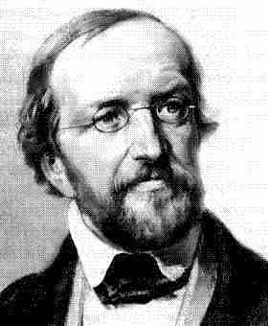
\includegraphics[width=.3\textwidth]{img/dirichlet}
	%From http://www-gap.dcs.st-and.ac.uk/~history/PictDisplay/Dirichlet.html
\end{center}

\begin{remark}
	Theorem~\ref{thm:units} is due to Dirichlet who lived 1805--1859.
	Thomas Hirst described Dirichlet thus:
	\begin{quote}
		He is a rather tall, lanky-looking man, with moustache and beard about
		to turn grey with a somewhat harsh voice and rather deaf. He was
		unwashed, with his cup of coffee and cigar. One of his failings is
		forgetting time, he pulls his watch out, finds it past three, and runs
		out without even finishing the sentence.
	\end{quote}
	Koch wrote that:
	\begin{quote}
		\dots important parts of mathematics were influenced by Dirichlet. His
		proofs characteristically started with surprisingly simple observations,
		followed by extremely sharp analysis of the remaining problem.
	\end{quote}
	I think Koch's observation nicely describes the proof we will give of
	Theorem~\ref{thm:units}.
\end{remark}

Units have a simple characterization in terms of their norm.
\begin{proposition}\label{prop:unitnorm}\iprop{unit norm characterization}
	An element $a \in \sO_K$ is a unit if and only if $\Norm_{K/\QQ}(a)=\pm 1$.
\end{proposition}
\begin{proof}
	Write $\Norm=\Norm_{K/\QQ}$.  If $a$ is a unit, then $a^{-1}$ is also a
	unit, and $1=\Norm(a)\Norm(a^{-1})$.  Since both $\Norm(a)$ and
	$\Norm(a^{-1})$ are integers, it follows that $\Norm(a)=\pm 1$.
	Conversely, if $a\in \sO_K$ and $\Norm(a)=\pm 1$, then the equation
	$aa^{-1}=1=\pm \Norm(a)$ implies that $a^{-1} = \pm \Norm(a)/a$.  But
	$\Norm(a)$ is the product of the images of~$a$ in $\CC$ by all
	embeddings of~$K$ into~$\CC$, so $\Norm(a)/a$ is also a product of
	images of~$a$ in~$\CC$, hence a product of algebraic integers,
	hence an algebraic integer. Thus $a^{-1} \in K \cap \overline{\ZZ} = \sO_K$,
	which proves that~$a$ is a unit.
\end{proof}

\begin{remark}
	Proposition~\ref{prop:unitnorm} is false if we replace $\sO_K$ by $K$.
	For example, if $\alpha$ is a root of $x^2-\frac{1}{2}x+1$, then
	$\alpha$ has norm $\pm 1$, but $\alpha$ is not a unit of $\sO_K$, since
	$\alpha \not\in \sO_K$.  To general Proposition~\ref{prop:unitnorm} to an
	arbitrary finite extension $R/S$ of Dedekind domains, we replace $\pm 1$
	by ``an element of $S^*$''.
\end{remark}

Let $r$ be the number of real and $s$ the number of complex conjugate
embeddings of $K$ into $\CC$, so $n = [K:\QQ] = r + 2s$.
Define the {\em log map}
\[
  \varphi:U_K \to \RR^{r+s}
\]
by
\[
  \varphi(a) = \left(
    \log\left|\sigma_1(a)\right|, \dots, \log\left|\sigma_{r+s}(a)\right|
  \right).
\]
Here $|z|$ is the usual absolute value of $z=x+iy \in \CC$
(so $|z|=\sqrt{x^2+y^2}$), and the maps $\sigma_i$ are
the same as those described in Lemma~\ref{lem:volok}.
In particular,
$\sigma_1,\dots,\sigma_r$ represent all real embeddings
$K\to\RR$ and $\sigma_{r+1},\dots,\sigma_{r+s}$ represent
half of the complex embeddings $K \to \CC$, with one representative
for each pair of complex conjugate embeddings.

\begin{lemma}\label{lem:inh}\ilem{hyperplane embedding}
  The image of $\varphi$ lies in the hyperplane
  \begin{equation}\label{eqn:hyperplane}
    H = \left\{ (x_1,\dots, x_{r+s}) \in \RR^{r+s} \colon
    x_1+ \cdots + x_r + 2x_{r+1} + \cdots + 2x_{r+s} = 0 \right\}.
  \end{equation}
\end{lemma}
\begin{proof}
  If $a\in U_K$, then by Proposition~\ref{prop:unitnorm},
  \[
    \left(\prod_{i=1}^{r} |\sigma_i(a)|\right)
    \cdot \left( \prod_{i=r+1}^{r+s} |\sigma_i(a)|^2 \right)
    = \left|\Norm_{K/\QQ}(a)\right|
    = 1.
  \]
  Taking logs of both sides proves the lemma.
\end{proof}

\begin{lemma}\label{lem:vphifinitekernel}
  The kernel of $\varphi$ is finite.
\end{lemma}
\begin{proof}
  We have
  \begin{align*}
    \ker(\varphi) &\subset \left\{a\in\sO_K \colon |\sigma_i(a)|
    = 1 \text{ for }i=1,\dots,r+s\right\} \\
    \sigma(\ker(\varphi)) &\subset \sigma(\sO_K) \cap X
  \end{align*}
  where $\sigma:\sO_K \to \CC^{r+s}$ is given by
  $\sigma(a) = \left(\sigma_1(a),\dots,\sigma_{r+s}(a)\right)$ and
  $X$ is the set $\left\{(z_1,\dots,z_{r+s}) \in \CC^{r+s} \colon |z_i|\leq 1\right\}$.
  Since $\sigma(\sO_K)$ is a lattice (see Proposition~\ref{prop:ok_lattice}) and $X$
  is compact, the intersection $\sigma(\sO_K)\cap X$ is finite.
  This implies $\ker(\varphi)$ is finite.
\end{proof}

\begin{lemma}\label{lem:kerfcg}
  The kernel of~$\varphi$ is a finite cyclic group.
\end{lemma}
\begin{proof}
  Lemma~\ref{lem:vphifinitekernel} implies that $\ker(\varphi)$ is a
  finite group.  It is a general fact that any finite subgroup $G$ of
  the multiplicative group $K^*$ of a field is cyclic (see
  Exercise~\ref{ex:finitesubgroupoffieldcyclic}).
\end{proof}

\begin{exercise}\label{ex:finitesubgroupoffieldcyclic}
  Finish the proof of Lemma~\ref{lem:kerfcg}
  by showing that for a field $K$, every finite
  subgroup $G$ of the multiplicative group $K^*$
  is cyclic.
  
  \begin{hint}
    Every element in $G$ satisfies a polynomial
    of the form $x^n-1$. Recall that a polynomial
    of degree $n$ over a field has at most $n$
    distinct roots. Now consider the orders
    of the elements of $G$.
  \end{hint}
\end{exercise}
%Proof:
%  If~$n$ is the exponent of~$G$, then every element of~$G$
%  is a root of the polynomial $x^n-1$. A polynomial of
%  degree~$n$ over a field has at most~$n$ roots, so $G$
%  has order at most~$n$, hence~$G$ is cyclic of order~$n$.

To prove Theorem~\ref{thm:units}, it suffices to prove that
$\Imag(\varphi)$ is a lattice in the hyperplane~$H$ of
(\ref{eqn:hyperplane}), which we view as a vector space of dimension
$r+s-1$.

Define an embedding
\begin{equation}\label{eqn:sigma3}
  \sigma : K \hookrightarrow \RR^n
\end{equation}
given by $\sigma(x) = (\sigma_1(x),\dots,\sigma_{r+s}(x))$,
where we view $\CC\isom \RR\times \RR$ via $a+b i\mapsto (a,b)$.
Thus this is the embedding
\begin{align*}
  x\mapsto \big(&\sigma_1(x), \sigma_2(x),\dots, \sigma_r(x), \\
  &\quad \Real(\sigma_{r+1}(x)), \Imag(\sigma_{r+1}(x)),
  \dots, \Real(\sigma_{r+s}(x)), \Imag(\sigma_{r+s}(x))\big).
\end{align*}

\begin{lemma}\label{lem:ukdiscrete}
  The image $\varphi:U_K\to \RR^{r+s}$ is discrete.
\end{lemma}
\begin{proof}
  Let $X$ be a bounded subset of $\RR^{r+s}$.
  We will show that the intersection $\varphi(U_K)\cap X$ is finite.
  Since $X$ is bounded, for any $u\in Y=\varphi^{-1}(X)\subset U_K$ the
  coordinates of $\sigma(u)$ are bounded, since $|\log(x)|$ is bounded on
  bounded subsets of $[1,\infty)$. Thus $\sigma(Y)$ is a bounded subset
  of $\RR^n$.  Since $\sigma(Y)\subset \sigma(\sO_K)$, and $\sigma(\sO_K)$ is
  a lattice in $\RR^n$, it follows that $\sigma(Y)$ is finite;
  moreover,~$\sigma$ is injective, so $Y$ is finite.
  Thus $\varphi(U_K)\cap X \subset \varphi(Y) \cap X$ is finite.
\end{proof}

We will use the following lemma in our
proof of Theorem~\ref{thm:units}.
\begin{lemma}\label{lem:chooseci}
  Let $n \geq 2$ be an integer, suppose $w_1,\dots,w_n \in \RR$
  are not all equal, and suppose $A, B \in \RR$ are positive. Then
  there exist $d_1,\dots,d_{n} \in \RR_{>0}$ such that
  \[
    \left|w_1\log(d_1)+\cdots +w_{n}\log(d_{n})\right| > B
  \]
  and $d_1\cdots d_n = A$.
\end{lemma}
\begin{proof}
  Order the $w_i$ so
  that $w_1\neq 0$.  By hypothesis there exists a $w_j$ such that
  $w_j\neq w_1$, and again re-ordering we may assume that $j=2$.  Set
  $d_3=\cdots=d_{r+s}=1$.  Suppose $d_1, d_2$ are any positive real numbers
  with  $d_1 d_2 = A$.  Since $\log(1)=0$,
  \begin{align*}
    \left|\sum_{i=1}^{n} w_i \log(d_i)\right|
    &= |w_1\log(d_1) + w_2\log(d_2)|\\
    &= |w_1 \log(d_1) + w_2\log(A/d_1)| \\
    &= |(w_1-w_2)\log(d_1) + w_2\log(A)|
  \end{align*}
  Since $w_1\neq w_2$,  we have $|(w_1-w_2)\log(d_1) + w_2\log(A)|\to\infty$
  as $d_1\to \infty$.  It is thus possible to choose the $d_i$ as in the lemma.
\end{proof}

\begin{proof}[Proof of Theorem~\ref{thm:units}]
  By Lemma~\ref{lem:ukdiscrete}, the image $\varphi(U_K)$ is discrete,
  so it remains to show that $\varphi(U_K)$ spans~$H$.
  Let~$W$ be the $\RR$-span of the image $\varphi(U_K)$, and note that $W$ is a
  subspace of~$H$, by Lemma~\ref{lem:inh}. 
  We will show that $W=H$ indirectly by showing that if $v\not \in H^{\perp}$,
  where~$\perp$ is the orthogonal complement with respect to the dot product
  on $\RR^{r+s}$, then $v\not \in W^{\perp}$.
  This will show that $W^{\perp}\subset H^{\perp}$, hence that $H\subset W$,
  as required.
  
  Thus suppose $z=(z_1,\dots,z_{r+s})\not\in H^{\perp}$.
  Define a function $f:K^*\to \RR$ by
  \begin{equation}\label{eqn:f}
    f(x) = z_1\log|\sigma_1(x)| + \cdots + z_{r+s}\log|\sigma_{r+s}(x)|.
  \end{equation}
  Note that $f(U_K)=\{0\}$ if and only if $z\in W^{\perp}$. So to show
  that $z\not\in W^{\perp}$, we show that there exists some $u\in U_K$
  with $f(u)\neq 0$.
  
  Let
  \[
    A=\sqrt{|d_K|} \cdot \left( \frac{2}{\pi}\right)^s \in \RR_{>0}.
  \]
  Choose any positive real numbers $c_1,\dots, c_{r+s} \in \RR_{>0}$ such that
  \[
    c_1\cdots c_r\cdot (c_{r+1}\cdots c_{r+s})^2 = A.
  \]
  Let $S$ be the of tuples $(x_1,\dots,x_n) \in \RR^n$ such that
  \[
    |x_i|\leq c_i\text{ for } 1\leq i \leq r
    \quad\text{ and }\quad
    |x_i^2 + x_{i+s}^2| \leq c_i^2 \text{ for } r<i\leq r+s.
  \]
  Then~$S$ is closed, bounded, convex, symmetric with respect to the
  origin, and of dimension $r+2s$, since $S$ is a product of~$r$ intervals
  and~$s$ discs, each of which has these properties. Viewing $S$ as a product
  of intervals and discs, we see that the volume of $S$ is
  \[
    \Vol(S)
    = \prod_{i=1}^r (2c_i) \cdot \prod_{i=1}^s (\pi c_i^2)
    = 2^r\cdot \pi^s \cdot A
    = 2^{r+s}\sqrt{|d_K|}
    = 2^n \cdot 2^{-s}\sqrt{|d_K|}.
  \]
  
  Recall Blichfeldt's Lemma~\ref{lem:blichfeld}, which asserts
  that if~$L$ is a lattice and~$S$ is closed, bounded, etc., and has volume
  at least $2^n\cdot \Vol(V/L)$, then $S\cap L$ contains a nonzero element.
  To apply this lemma, we take $L=\sigma(\sO_K)\subset \RR^n$, where $\sigma$
  is as in (\ref{eqn:sigma3}). By Lemma~\ref{lem:volok}, we have
  $\Vol(\RR^n/L) = 2^{-s}\sqrt{|d_K|}$. To check the hypothesis of
  Blichfeld's lemma, note that
  \[
    \Vol(S) = 2^n \cdot 2^{-s} \sqrt{|d_K|} = 2^n \Vol(\RR^n/L).
  \]
  Thus there exists a nonzero element $x$ in $S\cap \sigma(\sO_K)$.
  Let $a\in \sO_K$ with $\sigma(a)=x$, then $\sigma(a)\in S$, so
  $|\sigma_i(a)|\leq c_i$ for $1\leq i\leq r+s$. We then have
  \begin{align*}
    \left|\Norm_{K/\QQ}(a)\right|
    &= \left|\prod_{i=1}^{r+2s} \sigma_i(a)\right|
    \\
    &= \prod_{i=1}^r |\sigma_i(a)|\cdot \prod_{i=r+1}^s|\sigma_i(a)|^2
    \\
    &\leq c_1\cdots c_r\cdot (c_{r+1}\cdots c_{r+s})^2 = A.
  \end{align*}
  Since $a\in \sO_K$ is nonzero, we also have
  \[
    \left|\Norm_{K/\QQ}(a)\right|\geq 1.
  \]
  Moreover, if for any $i\leq r$, we have $|\sigma_i(a)|< \frac{c_i}{A}$, then
  \[
    1
    \leq \left|\Norm_{K/\QQ}(a)\right|
    < c_1\cdots \frac{c_i}{A}\cdots c_r \cdot (c_{r+1}\cdots c_{r+s})^2
    = \frac{A}{A} = 1,
  \]
  a contradiction, so $|\sigma_i(a)|\geq \frac{c_i}{A}$ for $i=1,\dots, r$.
  Likewise, $|\sigma_i(a)|^2 \geq \frac{c_i^2}{A}$, for $i=r+1,\dots, r+s$.
  Rewriting this we have
  \begin{equation}\label{eqn:cisigbound}
    \frac{c_i}{|\sigma_i(a)|}\leq A\quad\text{ for }i\leq r
    \quad\text{and}\quad
    \left(\frac{c_i}{|\sigma_i(a)|}\right)^2
    \leq A\quad\text{for } i=r+1,\dots, r+s.
  \end{equation}
  
  Recall that our overall strategy is to use an appropriately chosen~$a$
  to construct a unit $u\in U_K$ such $f(u)\neq 0$.  First, let
  $b_1,\dots, b_m$ be representative generators for the finitely many
  nonzero principal ideals of $\sO_K$ of norm at most $A$.  Since
  $\left|\Norm_{K/\QQ}(a)\right|\leq A$, we have $(a)=(b_j)$, for some $j$, so there
  is a unit~$u\in \sO_K$ such that $a=u b_j$.
  
  Let
  \[
    t = t_{c_1,\dots, c_{r+s}} = z_1\log(c_1)+\cdots +z_{r+s}\log(c_{r+s}),
  \]
  and recall $f:K^* \to \RR$ defined in (\ref{eqn:f}) above. We have
  \begin{align*}
    |f(u) - t| &= |f(a) - f(b_j) - t| \\
    &\leq |f(b_j)| + |t - f(a)| \\
    &=|f(b_j)| + \left|z_1(\log(c_1) - \log(|\sigma_1(a)|)) + \cdots + z_{r+s}(\log(c_{r+s}) - \log(|\sigma_{r+s}(a)|))\right|
    \\
    &=|f(b_j)| + \left|z_1\cdot \log(c_1/|\sigma_1(a)|) + \cdots + \frac{z_{r+s}}{2}\cdot \log((c_{r+s}/|\sigma_{r+s}(a)|)^2)\right|
    \\
    &\leq |f(b_j)| + \log(A)\cdot\left(\sum_{i=1}^{r}|z_i| + \frac{1}{2}\cdot \sum_{i=r+1}^s|z_i|\right)
    \overset{\text{def}}{=} B_j.
  \end{align*}
  In the last step we use (\ref{eqn:cisigbound}).
  
  Let $B=\max_{j} B_j$, and note that $B$ does not depend on the choice
  of the $c_i$; in fact, it only depends our {\em fixed} choice of $z$ and
  on the field $K$. Moreover, for any choice of the $c_i$ as above, we have
  \[
    |f(u) - t| \leq B.
  \]
  If we can choose positive real numbers~$c_i$ such that
  \begin{align*}
    c_1\cdots c_r\cdot (c_{r+1}\cdots c_{r+s})^2 &= A
    \\
    |t_{c_1,\dots, c_{r+s}}| &>B,
  \end{align*}
  then the fact that $|f(u)-t|\leq B$ would then imply that $|f(u)|>0$,
  which is exactly what we aimed to prove.
  
  If $r+s=1$, then we are trying to prove that $\varphi(U_K)$ is a lattice
  in $\RR^0 = \RR^{r+s-1}$, which is automatically true, so assume $r+s > 1$.
  To finish the proof, we explain how to use Lemma~\ref{lem:chooseci}
  to choose $c_i$ such that $|t|>B$. We have
  \begin{align*}
    t
    &= z_1\log(c_1)+\cdots + z_{r+s}\log(c_{r+s}) \\
    &= z_1\log(c_1)+\cdots + z_r\log(c_r)
    + \frac{1}{2}\cdot z_{r+1}\log(c_{r+1}^2) + \cdots
    + \frac{1}{2}\cdot z_{r+s}\log(c_{r+s}^2) \\
    &= w_1\log(d_1)+\cdots + w_r\log(d_r)+ w_{r+1}\log(d_{r+1}) +
    \cdots +\cdot w_{r+s}\log(d_{r+s}),
  \end{align*}
  where $w_i=z_i$ and $d_i=c_i$ for $i\leq r$, and
  $w_i=\frac{1}{2}z_i$ and $d_i=c_i^2$ for $r<i\leq r+s$.
  The condition that $z\not\in H^{\perp}$ is that the $w_i$ are not all
  the same, and in our new coordinates the lemma is equivalent to
  showing that $|\sum_{i=1}^{r+s} w_i \log(d_i)|>B$, subject to the
  condition that $\prod_{i=1}^{r+s} d_i = A$.
  But this is exactly what Lemma~\ref{lem:chooseci} shows. It is thus possible
  to find a unit~$u$ such that $|f(u)|>0$. Thus $z\not\in W^{\perp}$,
  so $W^{\perp}\subset H^{\perp}$, whence $H\subset W$,
  which finishes the proof of Theorem~\ref{thm:units}.
\end{proof}

\section{Examples with Sage}

\subsection{Pell's Equation}\label{sec:pell}

The so-called ``Pell's equation'' is $x^2 - dy^2 = 1$ with $d>0$ square
free, and we seek integer solutions $x,y$ to this equation.
If $x + y\sqrt{d} \in K = \QQ(\sqrt{d})$, then
\[
  \Norm(x+y\sqrt{d}) = (x + y\sqrt{d})(x - y\sqrt{d}) = x^2 -dy^2.
\]
Thus if $(x,y)$ are integers such that $x^2 - d y^2 = 1$, then
$\alpha = x + \sqrt{d}y \in \sO_K$ has norm $1$, so by
Proposition~\ref{prop:unitnorm} we have $\alpha \in U_K$.

\begin{exercise}
  Use Dirichlet's unit theorem to show that the solutions to Pell's equation
  form a finite-index subgroup of the group of units of $\QQ(\sqrt{d})$.
  Then show that the solutions modulo sign form an infinite cyclic group.
\end{exercise}

\begin{remark}
  The previous exercise takes substantial work to prove using only elementary
  number theory (for example, using continued fractions).
\end{remark}

We first solve Pell's equation $x^2 - 5y^2 = 1$ with $d=5$ by finding
the units of the ring of integers of $\QQ(\sqrt{5})$ using Sage.
Recall from Example~\ref{example:Qsqrt5ringofints} that the
ring of integers of $\QQ(\sqrt{5})$ is $\ZZ[\frac{1+\sqrt{5}}{2}]$

\begin{sagecode}
\begin{sagecell}
K.<sqrt5> = QuadraticField(5)
G = K.unit_group(); G
\end{sagecell}
\begin{sageout}
Unit group with structure C2 x Z of Number Field in sqrt5 with
defining polynomial x^2 - 5
\end{sageout}
\begin{sagecell}
u = G.1.value(); v = G.0.value(); (u, v)
\end{sagecell}
\begin{sageout}
(1/2*sqrt5 + 1/2, -1)
\end{sageout}
\end{sagecode} %link

The subgroup of cubes of $u$ gives us the units with integer $x,y$
(not both negative). \todo{is this remark relavent?}

\begin{sagecode} %link
\begin{sagecell}
[u^(3*i) for i in [0..9]]
\end{sagecell}
\begin{sageout}
[1, sqrt5 + 2, 4*sqrt5 + 9, 17*sqrt5 + 38, 72*sqrt5 + 161, \
305*sqrt5 + 682, 1292*sqrt5 + 2889, 5473*sqrt5 + 12238, \
23184*sqrt5 + 51841, 98209*sqrt5 + 219602]
\end{sageout}
\end{sagecode} %link

However, the norm of $u = \frac{1+\sqrt{5}}{2}$ is $-1$.
So the $6$th powers of $u$ will generate solutions to Pell's Equation.
We can also list the coefficients for these powers as follows.

\begin{sagecode} %link
\begin{sagecell}
[list(u^(6*i)) for i in [0..7]]
\end{sagecell}
\begin{sageout}
[[1, 0], [9, 4], [161, 72], [2889, 1292], [51841, 23184], \
[930249, 416020], [16692641, 7465176], [299537289, 133957148]]
\end{sageout}
\end{sagecode}

\begin{remark}
  A great article about Pell's equation is \cite{lenstra:pell}.  The
  MathSciNet review begins: ``This wonderful article begins with history
  and some elementary facts and proceeds to greater and greater depth
  about the existence of solutions to Pell equations and then later the
  algorithmic issues of finding those solutions. The cattle problem is
  discussed, as are modern smooth number methods for solving Pell
  equations and the algorithmic issues of representing very large
  solutions in a reasonable way.''
\end{remark}

The simplest solutions to Pell's equation can be huge, even when~$d$
is quite small. Read Lenstra's paper (cited in the above remark)
for some examples from over two thousand years ago.
Here is one example for $d=10000019$.

\begin{sagecode}
\begin{sagecell}
K.<a> = QuadraticField(next_prime(10^7))
G = K.unit_group(); G.1.value()
\end{sagecell}
\begin{sageout}
163580259880346328225592238121094625499142677693142915506747253000\
340064100365767872890438816249271266423998175030309436575610631639\
272377601680603795883791477817611974184075445702823789975945910042\
8895693238165048098039*a - \
517286692885814967470170672368346798303629034373575202975075605058\
714958080893991274427903448098643836512878351227856269086856679078\
304979321047765031073345259902622712059164969008633603603640331175\
6634562204182936222240930
\end{sageout}
\end{sagecode}

\begin{exercise}
  Let $U$ be the group of units of the ring of integers
  of $K=\QQ(\sqrt{5})$.
  \begin{enumerate}
    \item Prove that the set $S$ of units $x+y\sqrt{5} \in U$ with
    $x,y\in\ZZ$ is a subgroup of $U$.  (The main point is to show that
    the inverse of a unit with $x,y\in\ZZ$ again has coefficients in
    $\ZZ$.)
    \item Let $U^3$ denote the subgroup of cubes of elements of $U$.
    Prove that $S=U^3$ by showing that $U^3\subset S \subsetneq U$ and
    that there are no groups $H$ with $U^3\subsetneq H \subsetneq U$.
  \end{enumerate}
\end{exercise}

\subsection{Examples with Various Signatures}

In this section we give examples for various $(r,s)$ pairs.
First we consider $K=\QQ(i)$.
\begin{sagecode}
\begin{sagecell}
K.<a> = QuadraticField(-1)
K.signature()
\end{sagecell}
\begin{sageout}
(0, 1)
\end{sageout}
\begin{sagecell}
U = K.unit_group(); U
\end{sagecell}
\begin{sageout}
Unit group with structure C4 of Number Field in a with
defining polynomial x^2 + 1
\end{sageout}
\begin{sagecell}
U.0.value()
\end{sagecell}
\begin{sageout}
a
\end{sageout}
\end{sagecode}

The {\tt signature} method returns the number of real and complex conjugate
embeddings of $K$ into $\CC$. The {\tt unit\_group} method, which we used above,
returns the unit group $U_K$ as an abstract abelian group and a
homomorphism $U_K\to \sO_K$.

Next we consider $K=\QQ(\sqrt[3]{2})$.
\begin{sagecode}
\begin{sagecell}
K.<a> = NumberField(x^3 - 2)
K.signature()
\end{sagecell}
\begin{sageout}
(1, 1)
\end{sageout}
\begin{sagecell}
U = K.unit_group(); U
\end{sagecell}
\begin{sageout}
Unit group with structure C2 x Z of Number Field in a with
defining polynomial x^3 - 2
\end{sageout}
\begin{sagecell}
[u.value() for u in U.gens()]
\end{sagecell}
\begin{sageout}
[-1, a - 1]
\end{sageout}
\begin{sagecell}
u = U.1.value(); u
\end{sagecell}
\begin{sageout}
a - 1
\end{sageout}
\end{sagecode} %link

Below we use the {\tt places} command, which returns the real embeddings
and representatives for the complex conjugate embeddings.
We use the places to define the log map $\varphi$, which plays such a big
role in this chapter.
\begin{sagecode} %link
\begin{sagecell}
S = K.places(prec=53); S
\end{sagecell}
\begin{sageout}
[Ring morphism:
From: Number Field in a with defining polynomial x^3 - 2
To:   Real Double Field
Defn: a |--> 1.25992104989, \
Ring morphism:
From: Number Field in a with defining polynomial x^3 - 2
To:   Complex Double Field
Defn: a |--> -0.629960524947 + 1.09112363597*I]
\end{sageout}
\begin{sagecell}
def phi(z):
return [log(abs(sigma(z))) for sigma in S]
phi(u)
\end{sagecell}
\begin{sageout}
[-1.3473773483293832, 0.673688674164692]
\end{sageout}
\begin{sagecell}
phi(K(-1))
\end{sagecell}
\begin{sageout}
[0.0, 0.0]
\end{sageout}
\end{sagecode}
Note that $\varphi:U_K \to \RR^2$, and the image lands in the 1-dimensional
subspace of $(x_1,x_2)$ such that $x_1 +2x_2 = 0$.
Also, note that $\varphi(-1) = (0,0)$.

Let's try a field such that $r + s - 1 = 2$. First, one with $r=0$ and $s=3$:
\begin{sagecode}
\begin{sagecell}
K.<a> = NumberField(x^6 + x + 1)
K.signature()
\end{sagecell}
\begin{sageout}
(0, 3)
\end{sageout}
\begin{sagecell}
U = K.unit_group(); U
\end{sagecell}
\begin{sageout}
Unit group with structure C2 x Z x Z of Number Field in a with
defining polynomial x^6 + x + 1
\end{sageout}
\begin{sagecell}
u1 = U.1.value(); u1
\end{sagecell}
\begin{sageout}
a
\end{sageout}
\begin{sagecell}
u2 = U.2.value(); u2
\end{sagecell}
\begin{sageout}
a^3 + a
\end{sageout}
\begin{sagecell}
S = K.places(prec=53)
def phi(z):
return [log(abs(sigma(z))) for sigma in S]
phi(u1)
\end{sagecell}
\begin{sageout}
[-0.16741548328589614, 0.04864390975267338, 0.11877157353322298]
\end{sageout}
\begin{sagecell}
phi(u2)
\end{sagecell}
\begin{sageout}
[0.30678570892329504, -1.0725146505489758, 0.7657289416256803]
\end{sageout}
\begin{sagecell}
phi(K(-1))
\end{sagecell}
\begin{sageout}
[0.0, 0.0, 0.0]
\end{sageout}
\begin{sagecell}
sum(phi(u1))
\end{sagecell}
\begin{sageout}
2.220446049250313e-16
\end{sageout}
\begin{sagecell}
sum(phi(u2))
\end{sagecell}
\begin{sageout}
-4.440892098500626e-16
\end{sageout}
\end{sagecode}

Notice that the log image of $u_1$ is clearly not a real multiple of
the log image of $u_2$ (e.g., the scalar would have to be positive
because of the first coefficient, but negative because of the second).
This illustrates the fact that the log images of $u_1$ and $u_2$ span
a two-dimensional space.

Next we compute a field with $r=3$ and $s=0$.
(A field with $s=0$ is called \emph{totally real}.)
\begin{sagecode}
\begin{sagecell}
K.<a> = NumberField(x^3 + x^2 - 5*x - 1)
K.signature()
\end{sagecell}
\begin{sageout}
(3, 0)
\end{sageout}
\begin{sagecell}
U = K.unit_group(); U
\end{sagecell}
\begin{sageout}
Unit group with structure C2 x Z x Z of Number Field in a with
defining polynomial x^3 + x^2 - 5*x - 1
\end{sageout}
\begin{sagecell}
u1 = U.1.value(); u1
\end{sagecell}
\begin{sageout}
1/2*a^2 + a - 1/2
\end{sageout}
\begin{sagecell}
u2 = U.2.value(); u2
\end{sagecell}
\begin{sageout}
a
\end{sageout}
\begin{sagecell}
S = K.places(prec=53)
def phi(z):
return [log(abs(sigma(z))) for sigma in S]
phi(u1)
\end{sagecell}
\begin{sageout}
[-0.7747670223461895, -0.3928487245813982, 1.1676157469275887]
\end{sageout}
\begin{sagecell}
phi(u2)
\end{sagecell}
\begin{sageout}
[0.9966812040934553, -1.6402241503223172, 0.6435429462288627]
\end{sageout}
\end{sagecode}

A field with $r=0$ is called totally complex.  For
example, the \defn{cyclotomic fields} $\QQ(\zeta_n)$ are totally
complex, where $\zeta_n$ is a primitive $n$th root of
unity.  The degree of $\QQ(\zeta_n)$ over $\QQ$ is $\varphi(n)$ and $r=0$,
so $s=\varphi(n)/2$ (assuming $n>2$).
Here $\varphi$ is the Euler Totient function which on $n$
is defined as the number of integers $k$ such that $0<k\leq n$
and $\gcd(k,n)=1$.
\begin{sagecode}
\begin{sagecell}
K.<a> = CyclotomicField(11); K
\end{sagecell}
\begin{sageout}
Cyclotomic Field of order 11 and degree 10
\end{sageout}
\begin{sagecell}
K.signature()
\end{sagecell}
\begin{sageout}
(0, 5)
\end{sageout}
\begin{sagecell}
U = K.unit_group(); U
\end{sagecell}
\begin{sageout}
Unit group with structure C22 x Z x Z x Z x Z of \
Cyclotomic Field of order 11 and degree 10
\end{sageout}
\begin{sagecell}
u = U.1.value(); u
\end{sagecell}
\begin{sageout}
a^7 + a^6
\end{sageout}
\begin{sagecell}
S = K.places(prec=20)
def phi(z):
return [log(abs(sigma(z))) for sigma in S]
phi(u)
\end{sagecell}
\begin{sageout}
[-1.2566, -0.18533, 0.26982, 0.52028, 0.65180]
\end{sageout}
\begin{sagecell}
for u in U.gens():
print phi(u.value())
\end{sagecell}
\begin{sageout}
[0.00000, 0.00000, 0.00000, -9.5367e-7, 0.00000]
[-1.2566, -0.18533, 0.26982, 0.52028, 0.65180]
[-0.26981, -0.52028, 0.18533, -0.65180, 1.2566]
[0.65180, 0.26981, -1.2566, -0.18533, 0.52029]
[-0.084486, -1.1721, -0.33496, 0.60477, 0.98675]
\end{sageout}
\end{sagecode}


How far can we go computing unit groups of cyclotomic fields directly with Sage?
\begin{sagecode} %skip
\begin{sagecell}
%time U = CyclotomicField(11).unit_group()
\end{sagecell}
\begin{sageout}
CPU time: 0.01 s, Wall time: 0.01 s
\end{sageout}
\begin{sagecell}
%time U = CyclotomicField(13).unit_group()
\end{sagecell}
\begin{sageout}
CPU time: 0.30 s, Wall time: 0.30 s
\end{sageout}
\begin{sagecell}
%time U = CyclotomicField(17).unit_group()
\end{sagecell}
\begin{sageout}
CPU time: 1.13 s, Wall time: 1.31 s
\end{sageout}
\begin{sagecell}
%time U = CyclotomicField(23).unit_group()
\end{sagecell}
\begin{sageout}
.... I waited a few minutes and gave up....
\end{sageout}
\end{sagecode}

However, if you are willing to assume some conjectures (something
related to the Generalized Riemann Hypothesis), you can go further:
\begin{sagecode} %skip
\begin{sagecell}
proof.number_field(False)
%time U = CyclotomicField(11).unit_group()
\end{sagecell}
\begin{sageout}
CPU time: 0.07 s, Wall time: 0.07 s
\end{sageout}
\begin{sagecell}
%time U = CyclotomicField(13).unit_group()
\end{sagecell}
\begin{sageout}
CPU time: 0.03 s, Wall time: 0.03 s
\end{sageout}
\begin{sagecell}
%time U = CyclotomicField(17).unit_group()
\end{sagecell}
\begin{sageout}
CPU time: 0.06 s, Wall time: 0.06 s
\end{sageout}
\begin{sagecell}
%time U = CyclotomicField(23).unit_group()
\end{sagecell}
\begin{sageout}
CPU time: 0.26 s, Wall time: 0.31 s
\end{sageout}
\begin{sagecell}
%time U = CyclotomicField(29).unit_group()
\end{sagecell}
\begin{sageout}
CPU time: 0.60 s, Wall time: 0.62 s
\end{sageout}
\end{sagecode}

The generators of the units for $\QQ(\zeta_{29})$ are
\begin{align*}
  u_{0} &= -\zeta_{29}^{3}
  \\
  u_{1} &= \zeta_{29}^{26} + \zeta_{29}^{25} + \zeta_{29}^{22} + \zeta_{29}^{21} + \zeta_{29}^{19} + \zeta_{29}^{18} + \zeta_{29}^{15} + \zeta_{29}^{14} + \zeta_{29}^{11} + \zeta_{29}^{8} + \zeta_{29}^{7} + \zeta_{29}^{4} + \zeta_{29}^{3} + \zeta_{29} + 1
  \\
  u_{2} &= \zeta_{29}^{14} + \zeta_{29}^{3}
  \\
  u_{3} &= \zeta_{29}^{3} + 1
  \\
  u_{4} &= \zeta_{29}^{26} + \zeta_{29}^{20} + \zeta_{29}^{3}
  \\
  u_{5} &= \zeta_{29}^{22} + \zeta_{29}^{11} + \zeta_{29}^{2}
  \\
  u_{6} &= \zeta_{29}^{10} + \zeta_{29}^{9} + \zeta_{29}^{8}
  \\
  u_{7} &= \zeta_{29}^{23} + \zeta_{29}
  \\
  u_{8} &= \zeta_{29}^{17} + \zeta_{29}^{11}
  \\
  u_{9} &= \zeta_{29}^{22} + \zeta_{29}^{3}
  \\
  u_{10} &= \zeta_{29}^{24} + \zeta_{29}^{19} + \zeta_{29}^{5} + 1
  \\
  u_{11} &= \zeta_{29}^{19} + \zeta_{29}^{6}
  \\
  u_{12} &= \zeta_{29}^{27} + \zeta_{29}^{19} + \zeta_{29}^{11} + \zeta_{29}^{6} + \zeta_{29}^{3}
  \\
  u_{13} &= \zeta_{29}^{26} + \zeta_{29}^{15} + \zeta_{29}^{4}.
\end{align*}

There are better ways to compute units in cyclotomic fields than to
just use general purpose software. For example, there are explicit
{\em cyclotomic units} that can be written down and generate a finite
subgroup of $U_K$. See \cite[Ch.~8]{washington:cyclo}, which would be
a great book to read now that you've gone this far in the present book.
Also, using ideas explained in that book, it is probably
possible to make the {\tt unit\_group} command in Sage for cyclotomic
fields extremely fast, which would be an interesting project for a
reader who also likes to code.
\todo{has this been done? can you ask for sage contributions in a book?}
 % dirichlet
%%%%%%%%%%%%%%%%%%%%%%%%%%%%%%%%%%%%%%%%%%%%%%%%%%%%%%%%%%%%%%%%%%%%%%%%%%%
%% DECOMP
%%%%%%%%%%%%%%%%%%%%%%%%%%%%%%%%%%%%%%%%%%%%%%%%%%%%%%%%%%%%%%%%%%%%%%%%%%

\chapter{Decomposition and Inertia Groups}

In this chapter we will study extra structure in the case when~$K$
is Galois over~$\QQ$. We will learn about Frobenius elements,
the Artin symbol, decomposition groups, and how the Galois group of
$K$ is related to Galois groups of residue class fields. These are
the basic structures needed to attach $L$-functions to representations of
$\Gal(\overline{\QQ}/\QQ)$, which will play a central role in the next few chapters.

\section{Galois Extensions}

In this section we give a survey (no proofs) of the basic facts about
Galois extensions that will be needed in the rest of this chapter.
\begin{definition}[Galois]
  An extension $L/K$ of number fields is \defn{Galois} if
  \[
    \#\Aut(L/K) = [L:K],
  \]
  where $\Aut(L/K)$ is the group of automorphisms of $K$
  that fix $L$.  We write
  \[
    \Gal(L/K) = \Aut(L/K).
  \]
\end{definition}
For example, if $K \subset \CC$ is a number field embedded in the complex numbers,
then $K$ is \defn{Galois} over $\QQ$ if every field
homomorphism $K \to \CC$ has image $K$. As another example, any quadratic
extension $L/K$ is Galois over $K$, since it is of the form $K(\sqrt{a})$,
for some $a \in K$, and the nontrivial automorphism is induced
by $\sqrt{a} \mapsto -\sqrt{a}$, so there is always one nontrivial automorphism.
If $f \in K[x]$ is an irreducible cubic polynomial, and $\alpha$ is
a root of $f$, then one proves in a course on Galois theory that $K(\alpha)$
is Galois over $K$ if and only if the discriminant of~$f$ is a perfect square
in~$K$. ``Random'' number fields of degree bigger than $2$ are rarely Galois.

If $K \subset \CC$ is a number field, then the \defn{Galois closure} $\overline{K}$
of $K$ in $\CC$ is the field generated by all images of~$K$ under all
embeddings in~$\CC$ (more generally, if $L/K$ is an extension, the
Galois closure of $L$ over $K$ is the field generated by images of
embeddings $L \to \CC$ that are the identity map on $K$).

\begin{exercise}
  Suppose $K \subset \CC$ is a number field of the form $\QQ(\alpha)$ for some
  $\alpha \in \CC$. Show that $\overline{K}$ is generated (as an extension of $\QQ$)
  by all the conjugates of $\alpha$.
  %the image under an embedding of any
  %polynomial in the conjugates of~$\alpha$ is again a polynomial in
  %conjugates of $\alpha$.
\end{exercise}

How much bigger can the degree of $\overline{K}$ be as compared to the
degree of $K=\QQ(\alpha)$? There is an embedding of $\Gal(\overline{K}/\QQ)$
into the group of permutations of the conjugates of $\alpha$.
If $\alpha$ has $n$ conjugates, then this is an embedding
$\Gal(\overline{K}/\QQ) \hookrightarrow S_n$, where $S_n$ is the symmetric group on~$n$
symbols, which has order~$n!$. Thus the degree of the $\overline{K}$ over~$\QQ$
is a divisor of $n!$. Also $\Gal(\overline{K}/\QQ)$ is a transitive
subgroup of $S_n$, which constrains the possibilities further.
When $n=2$, we recover the fact that quadratic extensions are Galois.
When $n=3$, we see that the Galois closure of a cubic extension is either
the cubic extension or a quadratic extension of the cubic extension.
One can show that the Galois closure of a cubic extension is obtained
by adjoining the square root of the discriminant, which is why an
irreducible cubic defines a Galois extension if and only if the discriminant
is a perfect square.

For an extension $K$ of $\QQ$ of degree $5$, it is ``frequently'' the case that
the Galois closure has degree $120$, and in fact it is an interesting problem
to enumerate examples of degree~$5$ extensions in which the Galois closure
has degree smaller than $120$. For example, the only possibilities for the
order of a transitive proper subgroup of $S_5$ are $5$, $10$, $20$, and $60$;
there are also proper subgroups of $S_5$ order $2, 3, 4, 6, 8, 12$, and $24$,
but none are transitive.

\begin{exercise}
  Let $\alpha$ be a root of the irreducible polynomial $f(x) = x^5 - 6x + 3$ and
  let $K = \QQ(\alpha)$.
  \begin{enumerate}
    \item
    Use {\Sage} to verify that the Galois group $\Gal(\overline{K}/\QQ)$
    has order $120$.
    Warning: this command may take a long time to run.
    Try to finish the second part of this exercise before your code
    finishes.
    %%%time
    %R.<x> = ZZ[]
    %f = x^5 - 6*x + 3
    %K.<a> = NumberField(f)
    %Kgc.<b> = K.galois_closure()
  
    \item
    One can show that $f$ has three real roots and two complex roots.
    Show that $\Gal(\overline{K}/\QQ)$ contains an element of order $5$ and
    an element of order $5$. Use this to argue that $\Gal(\overline{K})/\QQ$
    has order $120$.
  \end{enumerate}
  \begin{hint}
    Number fields in {\Sage} have a {\tt galois\_closure()} command that
    returns the Galois closure of the field.
    For the second part, you want to show that any $5$-cycle and transposition
    will generate $S_5$.
  \end{hint}
\end{exercise}

\begin{example}
  Let $n$ be a positive integer. Consider the field $K=\QQ(\zeta_n)$,
  where $\zeta_n=e^{2\pi i/n}$ is a primitive $n$th root of unity.  If
  $\sigma:K\to \CC$ is an embedding, then $\sigma(\zeta_n)$ is also an
  $n$th root of unity, and the group of $n$th roots of unity is cyclic.
  So $\sigma(\zeta_n) = \zeta_n^m$ for some $m$ which is invertible
  modulo $n$.  Thus $K$ is Galois and $\Gal(K/\QQ) \hookrightarrow (\ZZ/n\ZZ)^*$.
  However, $[K:\QQ] = \varphi(n)$, so this map is an isomorphism.
\end{example}

\begin{remark}
  Taking a limit using the maps $\Gal(\overline{\QQ}/\QQ)\to
  \Gal(\QQ(\zeta_{p^r})/\QQ)$, we obtain a homomorphism $\Gal(\overline{\QQ}/\QQ)\to
  \ZZ_p^*$, which is called the {\em $p$-adic cyclotomic character}.
\end{remark}

Compositums of Galois extensions are Galois.  For example, the
biquadratic field $K=\QQ(\sqrt{5},\sqrt{-1})$ is a Galois
extension of $\QQ$ of degree~$4$, which is the compositum
of the Galois extensions $\QQ(\sqrt{5})$ and $\QQ(\sqrt{-1})$ of $\QQ$.

Fix a number field $K$ that is Galois over $\QQ$.
Then the Galois group acts on many of the objects
that we have associated to $K$.

\begin{exercise}\label{ex:galois-action-on-things}
  Let $L/K$ be a Galois extension of number fields, and let $G = \Gal(L/K)$.
  Describe the natural action of $G$ on the following objects:
  \begin{itemize}
    \item The ring of integers $\sO_K$.
    \item The group units $U_K$.
    \item The set of ideals of $\sO_K$.
    \item The group of fractional ideals of $\sO_K$.
    \item The class group $\Cl(K)$.
    \item The set $S_\p$ of prime ideals of $\sO_L$ lying over a given nonzero
    prime ideal $\p$ of $\sO_K$, i.e., the prime divisors of $\p\sO_L$.
  \end{itemize}
\end{exercise}

In the next section we will be concerned with the action of
$\Gal(L/K)$ on $S_\p$, though actions on each of the other objects,
especially $\Cl(L)$, are also of great interest. Understanding the
action of $\Gal(L/K)$ on $S_{\p}$ will enable us to associate, in a
natural way, a holomorphic $L$-function to any complex representation
$\Gal(L/K) \to \GL_n(\CC)$.

\section{Decomposition of Primes: $efg=n$}

Let $L/K$ be an extension of number fields and let $\p$ be a prime
in $\sO_K$. By Theorem~\ref{thm:intuniqfac} the ideal $\p\sO_L$ factors
uniquely into a product of primes of $\sO_L$ given by
\[
  \p\sO_L = \prod_{i=1}^g \P^{e_i}_i,
\]
where the $\q_i$ are the prime ideals of $\sO_L$ laying over $\p$, and
the $e_i$ are positive integers. The goal of this section is to study this
factorization. First we will introduce some standard terminology.

\begin{definition}[Ramification Index]
  The \defn{ramification index} of $\q_i$ over $\p$ is
  \[
    e(\P_i/\p) = e_i.
  \]
\end{definition}

\begin{definition}[Inertia degree]
  The \defn{inertia degree}
  of $\P_i$ over $\p$ is
  \[
    f(\P_i/\p) = \left[\sO_L/\P_i : \sO_K/\p\right].
  \]
\end{definition}

\begin{exercise}\label{ex:ramificationmultiplicative}
  The following properties follow quickly from the definitions.
  Let $M/L/K$ be a tower of number fields. Let $\p$ be a prime
  in $\sO_K$, $\q$ a prime in $\sO_L$ lying over $\p$, and $\P$ a prime
  in $\sO_M$ lying over $\q$.
  \begin{enumerate}
    \item[(a)] Show that $e(\P/\p)=e(\P/\q) \cdot e(\q/\p)$.
    \item[(b)] Show that $f(\P/\p)=f(\P/\q) \cdot f(\q/\p)$.
    \item[(c)] Let $g_{L/K}(\p)$, $g_{M/K}(\p)$ be the number of primes
    of $\sO_L$, $\sO_M$ lying over $\p$ respectively. Show that
    \[
      g_{M/K}(\p) = \sum\limits_{\q \text{ divides } \p\sO_L} g_{L/K}(\q).
    \]
  \end{enumerate}
\end{exercise}

Now suppose that $L/K$ is Galois and let $\sigma\in\Gal(L/K)$.
We saw in Exercise~\ref{ex:galois-action-on-things} that $\Gal(L/K)$ acts
naturally on the set $S_\p$ for a prime $\p$ of $\sO_K$.
This means that $\sigma(\P) \in S_\p$ for any $\P \in S_\p$. Moreover,
$\sigma$ induces an isomorphism of finite fields $\sO_L/\P\to \sO_L/\sigma(\P)$
that fixes the common subfield $\sO_K/\p$. Thus $\P$ and $\sigma(\P)$ have
the same inertia degree, i.e. $f(\P/\p) = f(\sigma(\P)/\p)$.
In fact, much more is true.

\begin{theorem}\label{thm:transitive}\ithm{transitive Galois action}
  Suppose $L/K$ is a Galois extension of number fields,
  and let $\p$ be a prime of $\sO_K$. 
  Write $\p\sO_K = \prod_{i=1}^g \P_i^{e_i}$, and let $f_i = f(\P_i/\p)$.
  Then $G = \Gal(L/K)$ acts transitively on the set $S_\p$ of primes $\P_i$,
  and
  \[
    e_1 = \cdots = e_g, \qquad f_1 = \cdots = f_g.
  \]
  Moreover, if we let $e$ be the common value of the $e_i$,
  $f$ the common value of the $f_i$, and $n = [K:L]$, then
  \[
    efg = n.
  \]
\end{theorem}
\begin{proof}
  For simplicity, we will give the proof only for an extension $K/\QQ$, but
  the proof works in general. Suppose $p \in \ZZ$ and
  $p\sO_K = \p_1^{e_1}\cdots \p_g^{e_g}$, and $S = \{\p_1,\ldots, \p_g\}$.  We
  will first prove that $G = \Gal(K/\QQ)$ acts transitively on $S$. 
  Let $\p = \p_i$ for some~$i$.
  Recall Lemma~\ref{lem:magica} which we proved long ago using the
  Chinese Remainder Theorem (Theorem~\ref{thm:crt}). It showed there exists
  $a\in\p$ such that $(a)/\p$ is an integral ideal that is
  coprime to $p\sO_K$.   The product
  \begin{equation}\label{eqn:prodquo}
    I = \prod_{\sigma\in G} \sigma((a)/\p)
    = \prod_{\sigma\in G} \frac{(\sigma(a))\sO_K}{\sigma(\p)}
    = \frac{(\Norm_{K/\QQ}(a))\sO_K}{\displaystyle \prod_{\sigma\in G} \sigma(\p)}
  \end{equation}
  is a nonzero integral $\sO_K$ ideal since it is a product of nonzero
  integral $\sO_K$ ideals.
  Since $a\in \p$ we have that
  $\Norm_{K/\QQ}(a) \in \p\cap\ZZ=p\ZZ$.  Thus the numerator of
  the rightmost expression in (\ref{eqn:prodquo}) is
  divisible by $p\sO_K$.   Also, because $(a)/\p$ is coprime
  to $p\sO_K$, each $\sigma((a)/\p)$ is coprime to $p\sO_K$
  as well.   Thus $I$ is coprime to $p\sO_K$.   This means the
  denominator of the rightmost expression in (\ref{eqn:prodquo})
  must also be divisible by $p\sO_K$ in order to cancel the $p\sO_K$
  in the numerator.  Thus we have shown that for any~$i$,
  \[
    \prod_{j=1}^g \p_j^{e_j}
    = p\sO_K \,\,\Big|\,\, \prod_{\sigma\in G} \sigma(\p_i).
  \]
  By unique factorization, since every $\p_j$ appears in the left hand
  side, we must have that for each~$j$ there is a~$\sigma$ with
  $\sigma(\p_i)=\p_j$, i.e., $G$ acts transitively on $S$.

  Choose some $j$ and suppose that $k\neq j$ is another index.  Because
  $G$ acts transitively, there exists $\sigma\in G$ such that
  $\sigma(\p_k)=\p_j$.  Applying $\sigma$ to the factorization $p\sO_K =
  \prod_{i=1}^g \p_i^{e_i}$, we see that
  \[
    \prod_{i=1}^g \p_i^{e_i} = \prod_{i=1}^g \sigma(\p_i)^{e_i}.
  \]
  Using unique factorization,
  we get $e_j = e_k$.  Thus $e_1=e_2=\cdots = e_g$.

  As was mentioned right before the statement of the theorem,
  for any $\sigma\in G$ we have $\sO_K/\p_i\isom \sO_K/\sigma(\p_i)$.
  Since $G$ acts transitively it follows that $f_1=f_2=\cdots = f_g$.
  We have, upon applying the Chinese Remainder Theorem
  and noting $\#(\sO_K/(\p^m)) = \#(\sO_K/\p)^m$
  (see Exercise~\ref{ex:residuefieldofpower}), that
  \begin{align*}
    [K:\QQ]&= \dim_{\ZZ} \sO_K = \dim_{\FF_p} \sO_K/p\sO_K \\
    &= \dim_{\FF_p} \left(\bigoplus_{i=1}^g \sO_K/\p_i^{e_i}\right)
    = \sum_{i=1}^g e_i f_i
    = efg,
  \end{align*}
  which completes the proof.
\end{proof}

\subsection{Examples}

This section gives examples illustrating the theorem for quadratic fields
and a cubic field and its Galois closure.

\subsubsection{Quadratic Extensions}

Suppose $K/\QQ$ is a quadratic field. 
Then $K$ is Galois, so for each prime $p\in\ZZ$ we have $2 = efg$.
There are exactly three possibilities for $e$, $f$ and $g$ :
\begin{description}
  \item[\normalfont{(Ramified):}] $e=2$, $f=g=1$: The prime $p$ \emph{ramifies} in
  $\sO_K$, which means $p\sO_K = \p^2$.  Let $\alpha$ be a generator for $\sO_K$ and
  $h \in \ZZ[x]$ a minimal polynomial for $\alpha$.
  By Theorem~\ref{thm:fac1} a prime $p$ is ramified in $\sO_K$ if and only if
  $h$ has a double root modulo~$p$, which is equivalent to $p$ dividing
  the discriminant of $h$. This shows there are only finitely many ramified
  primes.

  \item[\normalfont{(Inert):}] $e=1$, $f=2$, $g=1$: The prime $p$ is \emph{inert} in $\sO_K$,
  which means $p\sO_K = \p$ is prime.  It is a nontrivial theorem that
  this happens half of the time,
  as we will see illustrated below for a particular example.

  \item[\normalfont{(Split):}] $e=f=1$, $g=2$: The prime $p$ \emph{splits} in $\sO_K$,
  which means $p\sO_K = \p_1\p_2$ with $\p_1\neq \p_2$.  This happens the other
  half of the time.
\end{description}

\begin{example}\label{exam:decompQsqrt5}
  Let $K=\QQ(\sqrt{5})$, so $\sO_K=\ZZ[\gamma]$, where
  $\gamma=(1+\sqrt{5})/2$.  Then $p=5$ is ramified, since $5\sO_K =
  (\sqrt{5})^2$.  More generally, the order $\ZZ[\sqrt{5}]$ has index $2$
  in $\sO_K$, so for any prime $p\neq 2$ we can determine the
  factorization of $p$ in $\sO_K$ by finding the factorization of the
  polynomial $x^2-5\in \FF_p[x]$. The polynomial $x^2-5$ splits as a
  product of two distinct factors in $\FF_p[x]$ if and only if $e=f=1$
  and $g=2$. For $p\neq 2,5$ this is the case if and only if $5$ is a
  square in $\FF_p$, i.e., if $\Legendre{5}{p} = 1$, where $\Legendre{5}{p}$ is $+1$
  if $5$ is a square mod $p$ and $-1$ if $5$ is not.  By quadratic
  reciprocity,
  \[
    \Legendre{5}{p}
    = (-1)^{\frac{5-1}{2}\cdot \frac{p-1}{2}} \cdot \Legendre{p}{5}
    = \Legendre{p}{5}
    = \begin{cases}
      +1 & \text{ if } p \equiv \pm 1\pmod{5} \\
      -1 & \text{ if } p \equiv \pm 2\pmod{5}.
    \end{cases}
  \]
  Thus whether $p$ splits or is inert in
  $\sO_K$ is determined by the residue class of~$p$
  modulo $5$. It is a theorem of Dirichlet, which was massively
  generalized by Chebotarev, that $p \equiv \pm 1$ half the time
  and $p \equiv \pm 2$ the other half the time.\footnote{
  For the actual statement and a proof of this theorem,
  see \cite{neukirch1999} Theorem~VII.13.4.}
\end{example}

\subsubsection{The Cube Root of Two}

Suppose $K/\QQ$ is not Galois.
Then $e_i$, $f_i$, and~$g$ are defined for each prime $p \in \ZZ$,
but we need not have $e_1=\cdots=e_g$ or $f_1=\cdots =f_g$.  We do still have that
$\sum_{i=1}^g e_i f_i = n$, by the Chinese Remainder Theorem as used in
the proof of \autoref{thm:transitive}.
%also \cite[Thm.~21]{marcus1977number}
%or \cite[Prop.~I.8.2]{neukirch1999}

Consider the case where $K=\QQ(\sqrt[3]{2})$. We know that $\sO_K = \ZZ[\sqrt[3]{2}]$.  Thus
$2\sO_K = (\sqrt[3]{2})^3$, so for $2$ we have $e=3$ and $f=g=1$.

Working modulo $5$ we have
\[
  x^3 - 2 = (x+2)(x^2+3x+4) \in \FF_5[x],
\]
and the quadratic factor is irreducible.  Thus
\[
  5\sO_K = \left(5, \sqrt[3]{2} + 2\right) \cdot
  \left(5, \left(\sqrt[3]{2}\right)^2 + 3\sqrt[3]{2} + 4\right).
\]
Thus here $g = 2$, $e_1 = e_2 = 1$, $f_1=1$, and $f_2 = 2$.
Thus when $K$ is not Galois we need not have that the $f_i$
are all equal.

\subsection{Definitions and Terminology}

In the previous sections we used words like ``ramify'',
``inert'', and ``split'' to describe the decomposition
of a prime in an extension. This section will define these
terms which will be used in later sections.

Let $L/K$ be an extension of number fields of degree $n$,
and let $\p$ be a prime in $\sO_K$. Then $\p$ factors in $\sO_L$ as
\[
  \p\sO_L = \prod_{i=1}^g \P_i^{e_i}
\]
where the $\P_i$ ranger over the primes of $\sO_L$ laying over $\p$.

\begin{definition}\label{def:ramify}
  \todo{idef?}
  The prime $\p$ \emph{ramifies} in $L$ if $e_i > 1$ for some $1\leq i\leq g$.
  Otherwise $\p$ is \emph{unramified}.
  %in general, residue fields should be separable, neukrich 49
  If also $g = 1$ and $f_1 = 1$, then $\p$ is \emph{totally ramified}.
\end{definition}

\begin{definition}\label{def:inert}
  The prime $\p$ is \emph{inert} in $L$ if $\p\sO_L$ is prime.
  In this case we have $g = 1$ and $e_1 = 1$.
\end{definition}

\begin{definition}\label{def:split}
  The prime $\p$ \emph{splits} in $L$ if $g > 1$. If also $g = [L : K]$,
  then $\p$ \emph{splits completely} or is \emph{totally split}.
\end{definition}

\begin{exercise}[See {\cite[Ch.~4, Exercise~24]{marcus1977number}}]
  Prove the following properties.
  \begin{enumerate}
    \item[(a)] If $\p$ it totally ramified in $L$
    then it is totally ramified in $K$.

    \item[(b)] Let $L'$ be another extension of $K$.
    If $\p$ is totally ramified in $L$ and unramified in $L'$
    then $L\cap L' = K$.
  \end{enumerate}
\end{exercise}

\begin{exercise}
  Let $K$ be a number field and $d_K$ the discriminant of $K$
  Prove that a prime $p$ divides $d_K$ if and only if $p$ ramifies in $K$.

  \begin{hint}
    This is proved in many books, see for example
    \cite[Thm.~24]{marcus1977number} or \cite[Cor.~III.2.12]{neukirch1999}
  \end{hint}
\end{exercise}

\section{The Decomposition Group}

Suppose $K$ is a number field that is Galois over $\QQ$ with
group $G = \Gal(K/\QQ)$. Fix a prime $\p \subset \sO_K$ lying over $p \in \ZZ$.
\begin{definition}[Decomposition group]\label{def:decomp}
  The \defn{decomposition group} of $\p$ is the subgroup
  \[
    D_\p = \{\sigma \in G \colon \sigma(\p) = \p\} \subset G.
  \]
\end{definition}
Note that $D_\p$ is the stabilizer of $\p$ for
the action of $G$ on the set of primes lying over $p$.

It also makes sense to define decomposition groups for relative
extensions $L/K$, but for simplicity and to fix ideas in this section
we only define decomposition groups for a Galois extension $K/\QQ$.

Let $\FF_{\p} = \sO_K/\p$ denote the residue class field of $\p$.
In this section we will prove that there is an exact sequence
\[
  1\to I_\p \to D_\p \to \Gal(\FF_{\p}/\FF_p)\to 1,
\]
where $I_\p$ is the \defn{inertia subgroup} of $D_\p$, and $\#I_\p=e = e(\p/p)$.
The most interesting part of the proof is showing that the natural
map $D_\p\to  \Gal(\FF_{\p}/\FF_p)$ is surjective.
We will also discuss the structure of $D_\p$ and introduce
Frobenius elements, which play a crucial role in understanding Galois
representations.


Recall from Theorem~\ref{thm:transitive} that~$G$ acts transitively
on the set of primes~$\p$ lying over~$p$.
The orbit-stabilizer theorem implies that $[G:D_\p]$ equals the
cardinality of the orbit of~$\p$, which by Theorem~\ref{thm:transitive}
equals the number~$g$ of primes lying over~$p$, so $[G:D_\p]=g$.

\begin{lemma}\label{decompGpsConj}\ilem{decomposition groups are conjugate}
  The decomposition subgroups $D_\p$ corresponding to primes $\p$
  lying over a given $p$ are all conjugate as subgroups of~$G$.
\end{lemma}
\begin{proof}
  See Exercise~\ref{ex:decompGpsConj}.
\end{proof}

\begin{exercise}\label{ex:decompGpsConj}
  Prove Lemma~\ref{decompGpsConj}.

  \begin{hint}
    For $\sigma,\tau\in G$ you need to show
    $\tau D_\p \tau^{-1} = D_{\tau\p}$.
    Start by writing down what it means for $\sigma\in D_\p$
    and $\tau\sigma\tau^{-1}\in D_{\tau\p}$.
  \end{hint}
  %solution:
  %We have for each $\sigma, \tau \in G$, that
  %$$\tau^{-1}\sigma \tau\p = \p
  %\iff
  %\sigma\tau \p = \tau \p,
  %$$
  %so
  %$$
  %\sigma \in D_{\tau\p} \iff \tau^{-1}\sigma\tau\in D_\p.
  %$$
  %Thus
  %$$
  %\sigma \in D_\p \iff \tau \sigma \tau^{-1} \in D_{\tau \p},
  %$$
  %which shows $\tau D_{\p}\tau^{-1} = D_{\tau \p}$.
\end{exercise}

The decomposition group is useful because it allows us
to refine the extension $K/\QQ$ into a tower of extensions, such that at
each step in the tower we understand the splitting behavior
of the primes lying over~$p$.

Recall the correspondence between subgroups of the Galois group
$G$ and subfields of $K$. The fixed fields corresponding to the
decomposition and inertia subgroups have an important description
in terms of the splitting behavior of the prime $\p$.
We characterize the fixed field of $D=D_\p$ as follows.

\begin{proposition}\label{prop:nosplit}\iprop{fixed field characterization}
  The fixed field
  \[
    K^D = \left\{a \in K \colon \sigma(a) = a\text{ for all }\sigma \in D\right\}
  \]
  of $D$ is the smallest subfield $F \subset K$ such that
  there is a unique prime of $\sO_K$ lying over $\q = \p\cap\sO_F$.
\end{proposition}
\begin{proof}
  First suppose $F = K^D$, and note that by Galois theory
  $\Gal(K/F)\isom D$. By Theorem~\ref{thm:transitive}, the group $D$
  acts transitively on the primes of $K$ lying over $\q$.  One of
  these primes is $\p$, and $D$ fixes $\p$ by definition, so there is
  only one prime of $K$ lying over $\q$.
  Conversely, if $F\subset K$ is such that $\q$ lies under a unique prime
  in $K$, then $\Gal(K/F)$ fixes $\p$ (since it is the only
  prime over $\q$), so $\Gal(K/F) \subset D$, hence $K^D \subset F$.
\end{proof}

Thus $p$ does not split in going from $K^D$ to $K$---it does some
combination of ramifying and staying inert.
To fill in more of the picture, the following proposition asserts that $p$
splits completely and does not ramify in $K^D/\QQ$.

\begin{proposition}\label{prop:noresidue}\iprop{$e$, $f$, $g$}
  Fix a finite Galois extension~$K$ of~$\QQ$,
  let~$\p$ be a prime lying over~$p$ with decomposition group~$D$,
  and set $F = K^D$ and $\q = \p \cap \sO_F$.
  Let $g$ be the number of primes of $K$ lying over $p$.
  Then
  \[
    e(\q/p) = f(\q/p) = 1,
    \quad e(\p/p) = e(\p/\q),
    \quad f(\p/p) = f(\p/\q),
    \quad \text{and } g = [F : \QQ].
  \]
\end{proposition}
\begin{proof}
  As mentioned right after Definition~\ref{def:decomp}, the
  orbit-stabilizer theorem implies that $g = [G : D]$, and
  by Galois theory $[G : D] = [F : \QQ]$, so $g = [F : \QQ]$. By
  Proposition~\ref{prop:nosplit}, $\p$ is the only prime of $K$
  lying over $\q$ so by Theorem~\ref{thm:transitive},
  \begin{align*}
    e(\p/\q) \cdot f(\p/\q) = [K:F]
    &= \frac{[K:\QQ]}{[F:\QQ]}
    \\
    &= \frac{e(\p/p) \cdot f(\p/p) \cdot g}{[F:\QQ]}
    \\
    &= e(\p/p) \cdot f(\p/p).
  \end{align*}
  Now $e(\p/\q)\leq e(\p/p)$ and $f(\p/\q)\leq f(\p/p)$, so
  we must have $e(\p/\q)=e(\p/p)$ and $f(\p/\q)=f(\p/p)$.
  Since from Exercise~\ref{ex:ramificationmultiplicative} we have
  $e(\p/p) = e(\p/\q) \cdot e(\q/p)$ and $f(\p/q) = f(\p/\q) \cdot f(\q/p)$,
  it follows that $e(\q/p) = f(\q/p) = 1$.
\end{proof}

We summarize the results of the decomposition of a prime in the
tower $K \supseteq K^D \supseteq \QQ$ in Table~\ref{tbl:decompfield}.
This table shows the ramification indices, inertia degrees,
and the number of primes at each step of the tower.

\begin{table}[h!]
  \centering
  \begin{tabular}{ccc|cc}
    \text{Ramification ($e$)} & \text{Inertia ($f$)} & \text{Splitting ($g$)} & \text{Primes} & \text{Fields} \\
    \hline
    &  &  & $\p$ & $K$ \\
    $e(\p/p)$ & $f(\p/p)$ & $1$ & $\vert$ & $\vert$ \\
    &  &  & $\q$ & $K^D$ \\
    $1$ & $1$ & $[K^D : \QQ]$ & $\vert$ & $\vert$ \\
    &  &  & $p$ &  $\QQ$
  \end{tabular}
  \caption{Decomposition in the fixed field $K^D$.}
  \label{tbl:decompfield}
\end{table}

\begin{exercise}
  Give an example of each of the following:
  \begin{enumerate}
    \item A finite nontrivial Galois extension $K$
    of $\QQ$ and a prime ideal $\p$ such that $D_\p = \Gal(K/\QQ)$.
    \item A finite nontrivial Galois extension $K$ of
    $\QQ$ and a prime ideal $\p$ such that $D_\p$ has order~$1$.
    \item A finite Galois extension~$K$ of
    $\QQ$ and a prime ideal $\p$ such that $D_\p$ is not a normal
    subgroup of $\Gal(K/\QQ)$.
    \item A finite Galois extension $K$ of
    $\QQ$ and a prime ideal $\p$ such that $I_\p$ is not a normal
    subgroup of $\Gal(K/\QQ)$.
  \end{enumerate}
\end{exercise}

\subsection{Galois groups of finite fields}\label{sec:galoisfinite}

Each $\sigma \in D = D_\p$ acts in a well-defined
way on the finite field $\FF_\p = \sO_K/\p$, so we obtain
a homomorphism
\[
  \varphi: D_\p \to \Aut(\FF_\p/\FF_p).
\]
We pause for a moment and review a few basic properties of
extensions of finite fields. In particular, they turn out
to be Galois so the map $\varphi$ above is actually a map
$D_\p \to \Gal(\FF_\p/\FF_p)$.
The properties in this section are general properties
of Galois groups for finite fields.

\begin{definition}
  Let $k$ be any field of characteristic $p$.
  Define $\Frob_p: k \to k$ to be the homomorphism
  given by $a\mapsto a^p$. The map $\Frob_p$ is
  called the \emph{Frobenius} homomorphism.
\end{definition}

\begin{exercise}\label{ex:frob}
  \hfill
  \begin{enumerate}
    \item Show the map $\Frob_p$ is in fact a field homomorphism,
    that is $\Frob_p(a + b) = \Frob_p(a) + \Frob_p(b)$
    and $\Frob_p(ab) = \Frob_p(a)\Frob_p(b)$.
    \item Suppose $k = \FF_p$. Then show $\Frob_p = id$, i.e.,
    $a^p = a$ for any $a\in\FF_p$.
    \item Suppose $k = \FF_{q}$ where $q=p^f$ for some $f\geq 1$.
    Show that $\Frob_p:k\to k$ is an automorphism.
    \item Continuing the previous part, note that by
    Exercise~\ref{ex:finitesubgroupoffieldcyclic}, $k^*$ is cyclic.
    Let $a\in k$ be a generator for $k^*$,
    so $a$ has multiplicative order $p^f-1$ and $k = \FF_p(a)$.
    Show that
    \[
      \Frob_p^n(a) = a^{p^n} = a
      \quad\Leftrightarrow\quad (p^f - 1) \mid p^n - 1
      \quad\Leftrightarrow\quad f \mid n
    \]
  \end{enumerate}
\end{exercise}

\begin{remark}
  Exercise~\ref{ex:frob} shows that all finite fields
  are \emph{perfect}. For more on perfect fields see
  a standard abstract algebra text such as
  \cite{dummit2004abstract}.
\end{remark}

By Exercise~\ref{ex:frob}(b,c) the map $\Frob_p$ is an
automorphism of $\FF_\p$ fixing $\FF_p$ and hence defines
an element in $\Gal(\FF_\p/\FF_p)$. Let $f = f_{\p/p}$ be the residue
degree of $\p$, i.e., $f = [\FF_\p:\FF_p]$.
Exercise~\ref{ex:frob}(d) shows the order of $\Frob_p$ is~$f$.
Since the order of the automorphism group of a field extension
is at most the degree of the extension, we conclude that
$\Aut(\FF_\p/\FF_p)$ is generated by $\Frob_p$. This shows
$\Aut(\FF_\p/\FF_p)$ has order equal to the degree $[\FF_\p/\FF_p]$
so we conclude that $\FF_\p/\FF_p$ is Galois.
We summarize the discussion into the following theorem.

\begin{theorem}\label{thm:galoisgroupfinitefield}
  The extension $\FF_{\p}/\FF_p$ is Galois and moreover,
  $\Gal(\FF_{\p}/\FF_p)$ is generated by the Frobenius map
  $\Frob_p$ defined by $a\mapsto a^p$.
\end{theorem}

\begin{exercise}
  Prove that up to isomorphism there is
  exactly one finite field of each degree.

  \begin{hint}
    By Theorem~\ref{thm:galoisgroupfinitefield}
    all elements in a finite field satisfy an equation
    of the form $x^{p^f} - x$ where $p$ is the
    characteristic and $f$ is the degree over $\FF_p$.
  \end{hint}
\end{exercise}


\subsection{The Exact Sequence}\label{sec:exactseq}

Because $D_\p$ preserves $\p$, there is a natural reduction homomorphism
\[
  \varphi:D_\p \to \Gal(\FF_{\p}/\FF_p).
\]
\begin{theorem}\label{thm:redsurj}\ithm{reduction of Galois group}
  The homomorphism $\varphi$ is surjective.
\end{theorem}
\begin{proof}
  Let $D = D_\p$ and $\tilde{a} \in \FF_{\p}$ be an element
  such that $\FF_{\p} = \FF_p(\tilde{a})$.
  Lift $\tilde{a}$ to an algebraic integer $a\in \sO_K$, and let
  $h = \prod_{\sigma \in D}(x-\sigma(a))\in K^D[x]$.
  Let $\tilde{h}$ be the reduction of $h$ modulo~$\p$.
  Note that $h(a) = 0$ so $\tilde{h}(\tilde{a}) = 0$.

  Note that the coefficients of $h$ lie in $\sO_{K^D}$.
  By Proposition~\ref{prop:noresidue}, the residue field of $\sO_{K^D}$
  is $\FF_p$ so $\tilde{h} \in \FF_p[x]$.
  Therefore $\tilde{h}$ is a multiple of the minimal polynomial of
  $\tilde{a}$ over $\FF_p$. In particular, $\Frob_p(\tilde{a})$
  must also be a root of $\tilde{h}$.
  Since the roots of $\tilde{h}$ are of the form $\widetilde{\sigma(a)}$
  this shows that $\widetilde{\sigma(a)} = \Frob_p(\tilde{a})$
  for some $\sigma\in D$.
  Hence $\varphi(\sigma)(\tilde{a}) = \Frob_p(\tilde{a})$. Since elements
  of $\Gal(K_\p/\FF_p)$ are determined by their action on $\tilde{a}$
  by choice of $\tilde{a}$, it follows that $\varphi(\sigma) = \Frob_p$
  and hence $\varphi$ is surjective because $\Frob_p$
  generates $\Gal(\FF_{\p}/\FF_p)$.
\end{proof}

\begin{definition}[Inertia Group]
  The \defn{inertia group associated to $\p$}
  is the kernel $I_\p$ of the map $D_\p \to \Gal(\FF_{\p}/\FF_p)$.
\end{definition}
We have an exact sequence of groups
\begin{equation}\label{eqn:exact}
  1 \to I_\p \to D_\p \to \Gal(\FF_{\p}/\FF_p)\to 1.
\end{equation}
The inertia group is a measure of how $p$ ramifies in $K$.
\begin{corollary}\icor{order of inertia group}
  We have $\# I_\p = e = e(\p/p)$.
\end{corollary}
\begin{proof}
  The exact sequence (\ref{eqn:exact}) implies that
  $\#I_\p = \#D_\p / f$ where $f = f(\p/p) = [\FF_{\p} : \FF_p]$.
  Applying Propositions~\ref{prop:nosplit} and \ref{prop:noresidue}, we have
  \[
    \#D_\p = \left[K : K^D\right] = \frac{[K:\QQ]}{g} = \frac{efg}{g} = ef.
  \]
  Dividing both sides by $f$ proves the corollary.
\end{proof}

We have the following characterization of $I_\p$.
\begin{proposition}\label{prop:charip}\iprop{inertia group characterization}
  Let $K/\QQ$ be a Galois extension with group $G$,
  and let~$\p$ be a prime of $\sO_K$ lying
  over a prime~$p$.  Then
  \[
    I_\p = \left\{
    \sigma\in G \ \colon \sigma(a) \equiv a\pmod{\p}\text{ for all } a\in\sO_K
    \right\}.
  \]
\end{proposition}
\begin{proof}
  By definition $I_\p = \{\sigma\in D_\p \colon \sigma(a) \equiv
  a\pmod{\p}\text{ for all } a\in\sO_K\}$, so it suffices to show that
  if $\sigma\not\in D_\p$, then there exists $a\in\sO_K$ such that
  $\sigma(a) \not\equiv a\pmod{\p}$.  If $\sigma\not\in D_\p$, then
  $\sigma^{-1}\not\in D_\p$, so $\sigma^{-1}(\p)\neq \p$.  Since both
  are maximal ideals, there exists $a\in\p$ with
  $a\not\in\sigma^{-1}(\p)$, i.e., $\sigma(a)\not\in\p$.  Thus
  $\sigma(a) \not\equiv a\pmod{\p}$.
\end{proof}

\begin{exercise}
  Let $I = I_\p$ be the inertia subgroup as above. Show that
  \begin{enumerate}
    \item $K^I$ is the largest subfield of $K$ such that $p$ is unramified
    in $K^I$.
    \item $K^I$ is the smallest subfield of $K$ such that $\p$ is totally
    ramified over $\p \cap K^I$.
  \end{enumerate}
\end{exercise}

Figure~\ref{fig:splitting-of-p} summarizes the relationship between $I,D$,
and the splitting of $p$ in $K$. The dots on the left represent primes
lying over $p$. The size of the dot represents the inertia degree.
Compare this with Table~\ref{tbl:decompfield}.
\begin{figure}
  \centering
  \begin{tikzpicture}[scale = 1.5]
  \node at (1,0) (Q) {$\QQ$};
  \node at (1,2) (K^D) {$K^D$};
  \node at (1,4) (K^I) {$K^I$};
  \node at (1,6) (K) {$K$};

  \draw (K) -- (K^I) node[right,midway]{$e$};
  \draw (K^I) -- (K^D) node[right,midway]{$f$};
  \draw (K^D) -- (Q) node[right,midway]{$g$};

  \node at (3,5) (I) {$I$};
  \node at (3,3) (D/I) {$D/I \cong \Gal(K^I/K^D)$};
  \node at (0,4) (D) {$D$};

  \draw (K^D) to [out=-180,in=-90](D);
  \draw (D) to [out=90,in=180](K);

  \draw (K^D) to [out=0,in=-90](D/I);
  \draw (D/I) to [out=90,in=0](K^I);

  \draw (K^I) to [out=0,in=-90](I);
  \draw (I) to [out=90,in=0](K);

  \node[draw] at (5,5) (K^I-Qefg) {$f = g = 1$};
  \node[draw] at (5,3) (K^D-K^Iefg) {$e = g = 1$};
  \node[draw] at (5,1) (QK^Defg) {$e = f = 1$};

  \node at (-2,0) (p) {$p$};

  \node at (-2.5,2) (q1) {\huge$\boldsymbol{\cdot}$};
  \node at (-2.0,2) (q2) {\huge$\boldsymbol{\cdot}$};
  \node at (-1.5,2) (q3) {\huge$\boldsymbol{\cdot}$};

  \draw (p) -- (q1);
  \draw (p) -- (q2);
  \draw (p) -- (q3);

  \node at (-2.5,4) (P1) {\large$\bullet$};
  \node at (-2.0,4) (P2) {\large$\bullet$};
  \node at (-1.5,4) (P3) {\large$\bullet$};

  \draw (q1) -- (P1);
  \draw (q2) -- (P2);
  \draw (q3) -- (P3);

  \node at (-2.5,6) (Q1) {\large$\bullet^{\text{\large $e$}}$\!\!\!\!};
  \node at (-2.0,6) (Q2) {\large$\bullet^{\text{\large $e$}}$\!\!\!\!};
  \node at (-1.5,6) (Q3) {\large$\bullet^{\text{\large $e$}}$\!\!\!\!};

  \draw (P1) -- (Q1);
  \draw (P2) -- (Q2);
  \draw (P3) -- (Q3);
  \end{tikzpicture}
  \caption{Splitting of $p$ in a Galois extension $K/\QQ$.}
  \label{fig:splitting-of-p}
\end{figure}


\section{Frobenius Elements}

Suppose that $K/\QQ$ is a finite Galois extension with group $G$ and $p$ is a
prime such that $e = 1$ (i.e., an unramified prime). Then $I = I_\p = 1$ for
any $\p\mid p$, so the map $\varphi$ of Theorem~\ref{thm:redsurj} is a canonical
isomorphism $D_\p \isom \Gal(\FF_{\p}/\FF_p)$. By Section~\ref{sec:galoisfinite},
the group $\Gal(\FF_{\p}/\FF_p)$ is cyclic with canonical generator $\Frob_p$.
The \defn{Frobenius element} corresponding to $\p$ is $\Frob_\p \in D_\p$.
It is the unique (see Exercise~\ref{ex:frobunique}) element of $G$ such that
for all $a \in \sO_K$ we have
\[
  \Frob_\p(a) \equiv a^p\pmod{\p}.
\]

\begin{exercise}\label{ex:frobunique}
  With the notation above, prove that $\Frob_\p$ is unique.
  That is, if $\sigma$ satisfies $\sigma(a) \equiv a^p \pmod{\p}$
  for all $a\in\sO_K$ then $\sigma = \Frob_\p$.
  
  \begin{hint}
    First show $\sigma\in D_\p$, then argue as in
    the proof of Proposition~\ref{prop:charip}.
  \end{hint}
\end{exercise}


Just as the primes $\p$ and decomposition groups $D_\p$ are all
conjugate, the Frobenius elements corresponding to primes
$\p\mid p$ are all conjugate as elements of~$G$.

\begin{proposition}\iprop{conjugation of Frobenius}
  For each $\sigma \in G$, we have
  \[
    \Frob_{\sigma\p} = \sigma\Frob_\p\sigma^{-1}.
  \]
  In particular, the Frobenius elements lying over a given
  prime are all conjugate.
\end{proposition}
\begin{proof}
  Fix $\sigma\in G$. For any $a\in\sO_K$ we have
  $\Frob_\p(\sigma^{-1}(a)) - \sigma^{-1}(a)^p \in \p$.
  Applying~$\sigma$ to both sides, we see that
  $\sigma\Frob_\p(\sigma^{-1}(a)) - a^p \in \sigma\p$,
  so $\sigma\Frob_\p\sigma^{-1} = \Frob_{\sigma \p}$.
\end{proof}

Thus the conjugacy class of $\Frob_\p$ in $G$ is a well-defined
function of~$p$.  For example, if $G$ is abelian, then $\Frob_\p$ does
not depend on the choice of $\p$ lying over $p$ and we obtain a well
defined symbol $\Legendre{K/\QQ}{p} = \Frob_\p\in G$ called the \defn{Artin symbol}.
It extends to a homomorphism from the free abelian
group on unramified primes~$p$ to~$G$.
Class field theory (for~$\QQ$) sets up a natural bijection
between abelian Galois extensions of $\QQ$ and certain maps from
certain subgroups of the group of fractional ideals for~$\ZZ$ (i.e., $\QQ^*$).
We have just described one direction of this bijection, which associates to an
abelian extension the Artin symbol (which is a homomorphism).

The Kronecker-Weber theorem asserts that the abelian extensions of
$\QQ$ are exactly the subfields of the fields $\QQ(\zeta_n)$, as $n$
varies over all positive integers.  By Galois theory there is a
correspondence between the subfields of the field $\QQ(\zeta_n)$,
which has Galois group $(\ZZ/n\ZZ)^*$, and the subgroups of $(\ZZ/n\ZZ)^*$.
If $H \subseteq (\ZZ/n\ZZ)^*$ is the subgroup corresponding to
$K \subset \QQ(\zeta_n)$ then the Artin reciprocity map
$p\mapsto \Legendre{K/\QQ}{p}$ is given by $p\mapsto [p]\in (\ZZ/n\ZZ)^*/H$.

\begin{remark}
  Notice above that the $n$ used is not unique. That is,
  if~$K$ is an abelian extension of $\QQ$ then it lies in some~$\QQ(\zeta_n)$.
  But then it also lies inside of~$\QQ(\zeta_{dn})$ for any
  positive integer~$d$. However, a different choice of $n$
  would mean a different choice of $H$. However the
  quotient $(\ZZ/n\ZZ)^*/H$ used is not dependent on $n$
  since it is isomorphic to the Galois group of $K/\QQ$.
\end{remark}

\section{The Artin Conjecture}\label{sec:artin}

The Galois group $\Gal(\overline{\QQ}/\QQ)$ is an object of central importance
in number theory, and we can interpret much of number theory as the
study of this group.  A good way to study a group is to study how it
acts on various objects, that is, to study its representations.

Endow $\Gal(\overline{\QQ}/\QQ)$ with the topology which has as a basis of open neighborhoods
of the origin the subgroups $\Gal(\overline{\QQ}/K)$, where~{$K$ varies
over finite Galois extensions of~$\QQ$.
Fix a positive integer~$n$ and let $\GL_n(\CC)$ be the group of
$n\times n$ invertible matrices over~$\CC$ with the discrete topology.

\begin{warning}\label{warn:galqtopology}
  The topology on $\Gal(\overline{\QQ}/\QQ)$ is {\bf not} the topology induced
  by taking as a basis of open neighborhoods around the origin
  the collection of finite-index normal subgroups of $\Gal(\overline{\QQ}/\QQ)$,
  see \cite[Ch.~7]{milne:FT} or Exercise~\ref{ex:nonopensbgpfiniteindexgalq}.
  In particular, there exist nonopen normal subgroups of finite index which
  do not correspond to subgroups $\Gal(\overline{\QQ}/K)$ for some finite Galois
  extension $K/\QQ$.
\end{warning}

\begin{definition}
  A \defn{complex  $n$-dimensional representation} of $\Gal(\overline{\QQ}/\QQ)$
  is a continuous homomorphism
  \[
    \rho: \Gal(\overline{\QQ}/\QQ) \to \GL_n(\CC).
  \]
\end{definition}
For $\rho$ to be continuous means that if $K$ is the fixed
field of $\ker(\rho)$, then $K/\QQ$ is a finite Galois extension.
We have a diagram
\[
  \begin{tikzcd}
  \Gal(\overline{\QQ}/\QQ) \arrow{rr}{\rho} \arrow{dr} & & \GL_n(\CC) \\
  & \Gal(K/\QQ) \arrow[hook]{ur}[swap]{\rho'}
  \end{tikzcd}
\]

\begin{exercise}\label{ex:galqrepfiniteimage}
  Suppose $\rho:\Gal(\overline{\QQ}/\QQ)\to\GL_n(\CC)$ is continuous.
  Show that the image is finite.
\end{exercise}

\begin{remark}
  The converse to Exercise~\ref{ex:galqrepfiniteimage}
  is \textbf{false} in general (see
  Exercise~\ref{ex:nonopensbgpfiniteindexgalq}).
  This is essentially the same warning as
  Warning~\ref{warn:galqtopology}, however it is worth
  pointing out to avoid mistakes.\footnote{
  See \cite[pg.~1]{artinconjectureLectureNotes}.}
\end{remark}

\begin{exercise}\label{ex:nonopensbgpfiniteindexgalq}
  Find a nonopen subgroup of index $2$ in $\Gal(\overline{\QQ}/\QQ)$.
  Note this is also an example of a non-continuous
  homomorphism $\Gal(\overline{\QQ}/\QQ)\to\GL_n(\CC)$ with finite image.

  \begin{hint}
    Use Zorn's lemma to show that there are homomorphisms
    $\Gal(\overline{\QQ}/\QQ)\to\{\pm 1\}$ with finite image that are not continuous,
    since they do not factor through the Galois group of any
    finite Galois extension.
  \end{hint}

  %  \begin{hint}
  %    The extension $\QQ(\sqrt{d}, d \in \QQ^*/(\QQ^*)^2)$
  %    is an extension of~$\QQ$ with Galois group $X\ncisom \prod \FF_2$.
  %    The index-two open subgroups of~$X$ correspond to the quadratic
  %    extensions of~$\QQ$. However, Zorn's lemma implies that~$X$
  %    contains many index-two subgroups that do not correspond to
  %    quadratic extensions of~$\QQ$.
  %  \end{hint}
\end{exercise}

\begin{exercise}
  Let $S_3$ by the symmetric group on three symbols, which has order $6$.
  \begin{enumerate}
    \item \label{ex:a} Observe that $S_3\isom D_3$, where $D_3$ is
    the dihedral group of order $6$, which is the group of symmetries of
    an equilateral triangle.
    \item Use (\ref{ex:a}) to write down an explicit
    embedding $S_3 \hookrightarrow \GL_2(\CC)$.
    \item Let $K$ be the number field $\QQ(\sqrt[3]{2},\omega)$,
    where $\omega^3=1$ is a nontrivial cube root of unity.  Show
    that $K$ is a Galois extension with Galois group isomorphic to~$S_3$.
    \item We thus obtain a $2$-dimensional irreducible complex
    Galois representation
    \[
      \rho:\Gal(\overline{\QQ}/\QQ) \to \Gal(K/\QQ) \isom S_3 \subset \GL_2(\CC).
    \]
    Compute a representative matrix of $\Frob_p$ and the characteristic polynomial
    of $\Frob_p$ for $p=5,7,11,13$.
  \end{enumerate}
\end{exercise}

Fix a Galois representation~$\rho$ and let $K$ be the fixed field of
$\ker(\rho)$, so~$\rho$ factors through $\Gal(K/\QQ)$.  For each prime
$p \in \ZZ$ that is not ramified in $K$, there is an element
$\Frob_\p\in\Gal(K/\QQ)$ that is well-defined up to conjugation by
elements of $\Gal(K/\QQ)$.  This means that $\rho'(\Frob_p)\in
\GL_n(\CC)$ is well-defined up to conjugation.  Thus the characteristic
polynomial $F_p(x) \in \CC[x]$ of $\rho'(\Frob_p)$ is a well-defined
invariant of $p$ and $\rho$.  Let
\[
  R_p(x)
  = x^{\deg(F_p)}\cdot F_p(1/x)
  = 1 + \cdots + \det(\Frob_p)\cdot x^{\deg(F_p)}
\]
be the polynomial obtain
by reversing the order of the coefficients of $F_p$.
Following E.~Artin \cite{artin:conjecture, artin:conjecture2}, set
\begin{equation}\label{eqn:artin}
  L(\rho,s) = \prod_{p\text{ unramified}}\frac{1}{R_p(p^{-s})}.
\end{equation}
We view $L(\rho,s)$ as a function of a single complex variable $s$.
One can prove that $L(\rho,s)$ is holomorphic on some right
half plane, and extends to a meromorphic function on all $\CC$.
\begin{conjecture}[Artin]\label{conj:artin}
  The $L$-function of any continuous representation
  \[
    \Gal(\overline{\QQ}/\QQ) \to \GL_n(\CC)
  \]
  is an entire function on all $\CC$, except possibly at $1$.
\end{conjecture}
This conjecture asserts that there is some way to analytically continue
$L(\rho,s)$ to the whole complex plane, except possibly at $1$.
(A standard fact from complex analysis is that this analytic
continuation must be unique.)
The simple pole at $s=1$ corresponds to the trivial representation (the
Riemann zeta function), and if $n\geq 2$ and $\rho$ is irreducible,
then the conjecture is that $\rho$ extends to a holomorphic function
on all $\CC$.

The conjecture is known when $n=1$.  Assume for the rest of this
paragraph that $\rho$ is odd, i.e., if $c\in\Gal(\overline{\QQ}/\QQ)$ is complex
conjugation, then $\det(\rho(c))=-1$.  When $n=2$ and the image of
$\rho$ in $\PGL_2(\CC)$ is a solvable group, the conjecture is known,
and is a deep theorem of Langlands and others (see
\cite{langlands:basechange}), which played a crucial roll in Wiles's
proof of Fermat's Last Theorem.  When $n=2$ and the image of $\rho$ in
$\PGL_2(\CC)$ is not solvable, the only possibility is that the
projective image is isomorphic to the alternating group~$A_5$.
Because~$A_5$ is the symmetry group of the icosahedron, these
representations are called \defn{icosahedral}.  In this case, Joe
Buhler's Harvard Ph.D. thesis \cite{buhler:thesis} gave the first
example in which $\rho$ was shown to satisfy
Conjecture~\ref{conj:artin}.  There is a book \cite{mr95i:11001},
which proves Artin's conjecture for 7 icosahedral representation (none
of which are twists of each other).  Kevin Buzzard and the author
proved the conjecture for 8 more examples \cite{buzzard-stein:artin}.
Subsequently, Richard Taylor, Kevin Buzzard, Nick Shepherd-Barron, and
Mark Dickinson proved the conjecture for an infinite class of
icosahedral Galois representations (disjoint from the examples)
\cite{bdsbt}.  The general problem for $n=2$ is in fact now completely
solved, due to recent work of Khare and Wintenberger
\cite{khare-wintenberger:serre1} that proves Serre's conjecture.
 % decomp
%%%%%%%%%%%%%%%%%%%%%%%%%%%%%%%%%%%%%%%%%%%%%%%%%%%%%%%%%%%%%%%%%%%%%%%%%%%
%% GALREP
%%%%%%%%%%%%%%%%%%%%%%%%%%%%%%%%%%%%%%%%%%%%%%%%%%%%%%%%%%%%%%%%%%%%%%%%%%

\chapter[Elliptic Curves and $L$-functions]{
  Elliptic Curves, Galois Representations, and $L$-functions
}

This chapter is about elliptic curves and the central role they play
in algebraic number theory.  Our approach will be less systematic and
more a survey than most of the rest of this book.  The goal is to
give you a glimpse of the forefront of research by assuming many basic
facts that can be found in other books (see, e.g.,
\cite{silverman:aec}).

\section{Groups Attached to Elliptic Curves}

\begin{definition}[Elliptic Curve]\label{defn:ec}
  An \defn{elliptic curve} over a field~$K$ is a genus one curve~$E$
  defined over~$K$ equipped with a distinguished point $\sO \in E(K)$.
  Here $E(K)$ is the set of all points on $E$ defined over $K$.
\end{definition}

We will not define \emph{genus} in this book, except to note that a
nonsingular curve over~$K$ has genus one if and only if over~$\overline{K}$
it can be realized as a nonsingular plane cubic curve.\footnote{
  For a detailed and technical explanation of genus
  see \cite[Ch.~II.8]{hartshorne} or
  \cite[Ch.~7.3]{liu2006algebraic}
}
Moreover, one
can show (using the Riemann-Roch formula) that over any field a genus
one curve with a rational point can always be defined by a projective
cubic equation of the form
\[
  Y^2 Z + a_1 XYZ + a_3 YZ^2 = X^3  + a_2 X^2Z + a_4 XZ^2 + a_6 Z^3.
\]
In this form the distinguished point $\sO$ is $(X:Y:Z) = (0:1:0)$.
Note that $\sO$ is the only point on the curve with $Z=0$. So we
can consider the rest of the curve in the affine coordinates
by projecting onto the affine plane defined by $Z\neq 0$.
This gives the equation
\begin{equation}\label{weq}
  y^2 +a_1 xy + a_3 y = x^3 + a_2 x^2 + a_4 x + a_6.
\end{equation}
Thus one often presents an elliptic curve by giving a
\emph{Weierstrass equation} (\ref{weq}), though there are significant
computational advantages to other equations for curves
(e.g., Edwards coordinates -- see work of Bernstein and Lange in
\cite{bernstein2007inverted}).

\begin{exercise}
  Look up the Riemann-Roch theorem in a book on algebraic curves
  (e.g. \cite{hartshorne,liu2006algebraic}).
  \begin{enumerate}[label=(\alph*)]
    \item Write it down in your own words.
    \item Let $E$ be an elliptic curve over a field~$K$.
    Use the Riemann-Roch theorem to deduce that the natural map
    \[
      E(K) \to \Pic^0(E/K)
    \]
    is an isomorphism.
  \end{enumerate}
\end{exercise}

Using {\Sage} we plot an elliptic curve over the finite field $\FF_7$ and an
elliptic curve defined over $\QQ$.
\begin{sagecode} %skip
\begin{sagecell}
E = EllipticCurve(GF(7), [1,0])
E
\end{sagecell}
\begin{sageout}
Elliptic Curve defined by y^2 = x^3 + x over
Finite Field of size 7
\end{sageout}
\end{sagecode}
\begin{sagecode}
\begin{sagecell} %skip
E.plot(pointsize=60, gridlines=True)
\end{sagecell}
\begin{sageout}[escapechar=!]
!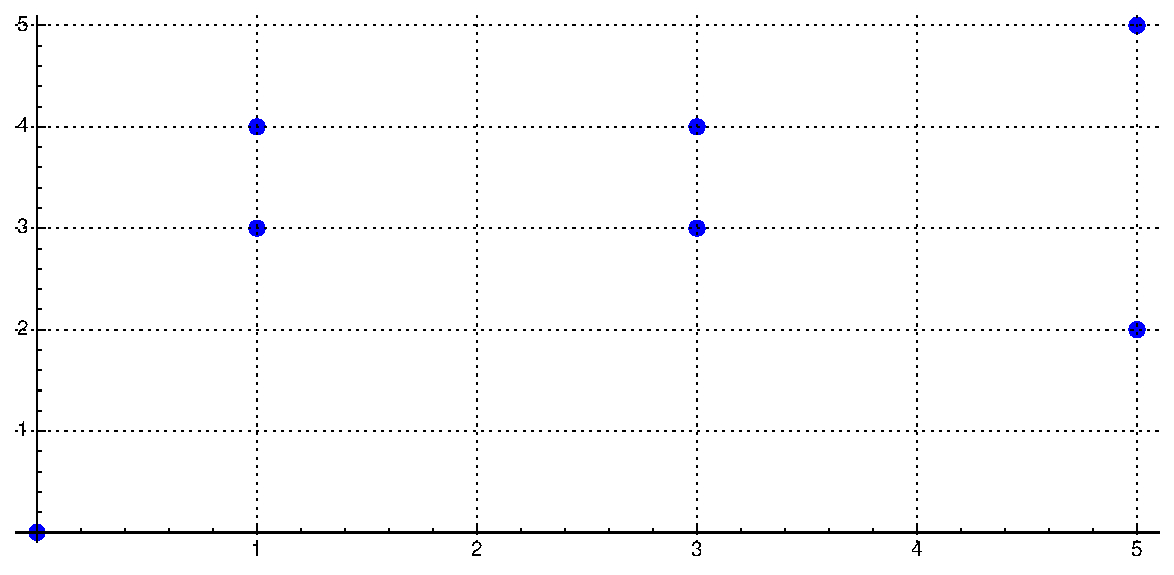
\includegraphics[width=0.9\textwidth]{img/ecmod7}
\end{sageout}
\end{sagecode}

\begin{sagecode}
\begin{sagecell}
E = EllipticCurve([1,0])
E
\end{sagecell}
\begin{sageout}
Elliptic Curve defined by y^2 = x^3 + x over
Rational Field
\end{sageout}
\end{sagecode}
\begin{sagecode}
\begin{sagecell} %skip
E.plot()
\end{sagecell}
\begin{sageout}[escapechar=!]
!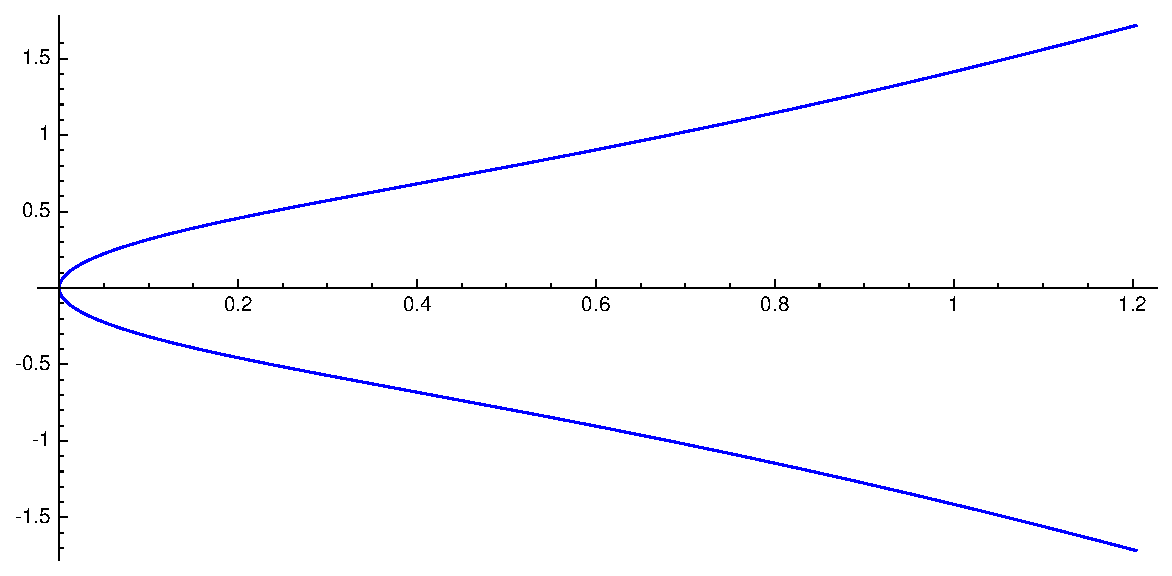
\includegraphics[width=0.9\textwidth]{img/ecq}
\end{sageout}
\end{sagecode}

Note that both plots above are of the affine equation $y^2 = x^3 + x$, and do
not include the distinguished point $\sO$, which lies at infinity.

\begin{remark}
  The command {\tt{EllipticCurve}} in {\Sage}
  can take as input a list {\tt{[a4,a6]}}
  of coefficients and returns an elliptic curve given
  by a Weirstrass equation with $a_1=a_2=a_3=0$ and
  $a_4,a_6$ as specified.
\end{remark}

\subsection{Abelian Groups Attached to Elliptic Curves}

If $E$ is an elliptic curve over~$K$, then we give the set
$E(K)$ of all $K$-rational points on~$E$ the structure of abelian
group with identity element~$\sO$.\footnote{
  As a reminder, we will not give rigorous proofs of any facts in
  this section. For a more detailed and technical explanation of
  the group structure for elliptic curves
  see \cite[Ch.~III.2]{silverman:aec}.
}
If we embed $E$ in the projective plane, then this group is determined
by the condition that three points sum to the zero element $\sO$
if and only if they lie on a common line (some care needs to be taken
when the points are not distinct). In our affine picture, a line will
intersect the point at infinity if it is vertical, or equivalently if
it of the form $x=a$ for some fixed $a\in K$.


\begin{example}\label{ex:ecgplaw}
  On the curve $y^2=x^3-5x+4$, we have $(0,2) + (1,0) = (3,4)$.
  This is because $(0,2)$, $(1,0)$, and $(3,-4)$ are on a common line
  (given by the equation $y = 2 - 2x$) hence they sum to zero:
  \[
    (0,2) + (1,0) + (3,-4) = \sO.
  \]
  Notice $(3,4)$, $(3,-4)$, and $\sO$ (the point at infinity on the curve)
  are also on a common line (given by $x = 3$), so $(3,4)=-(3,-4)$.
  We can illustration this in {\Sage}:
\begin{sagecode}
\begin{sagecell}
E = EllipticCurve([-5,4])
E(0,2) + E(1,0)
\end{sagecell}
\begin{sageout}
(3 : 4 : 1)
\end{sageout}
\end{sagecode} %link
\begin{sagecode}
\begin{sagecell} %skip
G = E.plot()
G += points ([(0,2) , (1,0) , (3,4) , (3,-4)],
pointsize=90 , color='red', zorder=10)
G += line ([(-1,4) , (4,-6)] , color='black')
G += line ([(3,-6) , (3,6)] , color='black')
G.show()
\end{sagecell}
\begin{sageout}[escapechar=!] %skip
!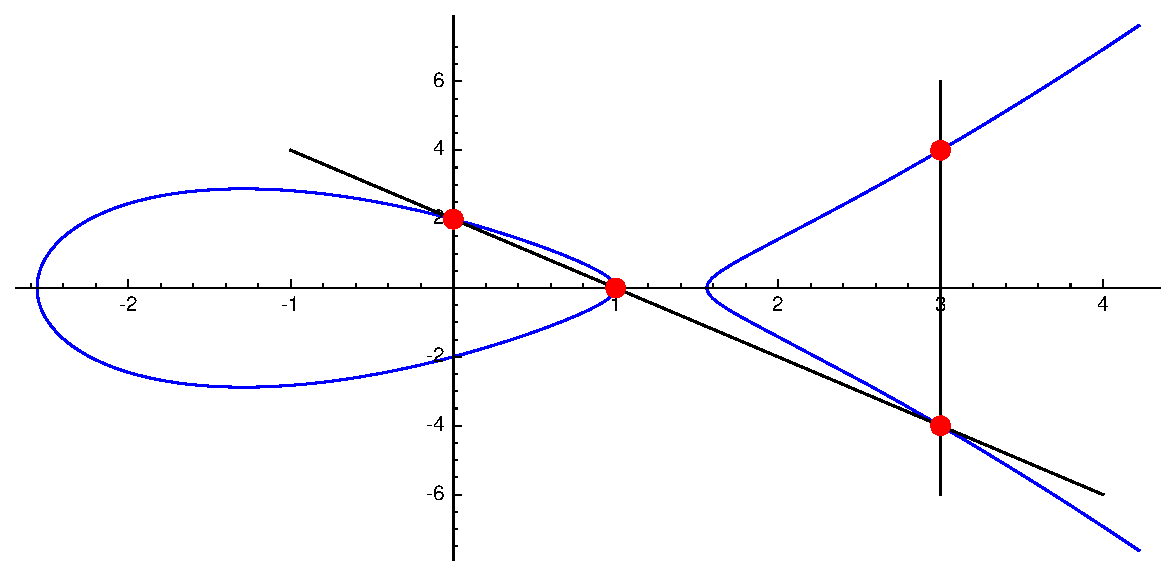
\includegraphics[width=0.925\textwidth]{img/grouplaw}
\end{sageout}
\end{sagecode} %link

  \noindent
  Iterating the group operation often leads quickly to
  very complicated points:

\begin{sagecode}
\begin{sagecell}
7*E(0,2)
\end{sagecell}
\begin{sageout}
(14100601873051200/48437552041038241 :
-17087004418706677845235922/10660394576906522772066289 :
1)
\end{sageout}
\end{sagecode}
\end{example}

\begin{remark}
  In the previous example we saw that iterating the
  group operation led to points which used a lot of digits
  to write down. This notion can be made formal and is called
  the \emph{height} of the point. The height function is used
  to prove the general Mordell-Weil theorem, see
  \cite[Ch.~VIII.4]{silverman:aec}
\end{remark}

\begin{exercise}\label{ex:ec2torsion}
  Let $E$ be an elliptic curve given by a
  Weirstrass equation such as (\ref{weq}) with $a_1=a_3=0$.
  Show that the points of order two are exactly
  the points on $E$ with $y$-coordinate equal to
  $0$.

  \begin{hint}
    Recall that a point $P$ has order $2$ if
    $P + P + \sO = \sO$, which means the tangent line
    at $P$ goes through the point at infinity.
  \end{hint}
\end{exercise}

That the above condition---three points on a line sum to
zero---defines an abelian group structure on $E(K)$ is not obvious.
Depending on your perspective, the trickiest part is seeing that the
operation satisfies the associative axiom.  The best way to understand
the group operation on $E(K)$ is to view $E(K)$ as being related to a
class group.  As a first observation, note that the ring
\[
  R = K[x,y]/(y^2 +a_1 xy + a_3 y - (x^3 + a_2 x^2 + a_4 x + a_6))
\]
is a Dedekind domain, so $\Cl(R)$ is defined, and every nonzero
fractional ideal can be written uniquely in terms of prime ideals.
When $K$ is a perfect field, the prime ideals correspond to the Galois
orbits of affine points of $E(\overline{K})$.
Note that these do not include the point at infinity.

Let $\Div(E/K)$ be the free abelian group on the Galois orbits of
points of~$E(\overline{K})$, which as explained above is analogous to
the group of fractional ideals of a number field (here we {\em do}
include the point at infinity).
We call the elements of $\Div(E/K)$
{\em divisors}.  Let $\Pic(E/K)$ be the quotient of $\Div(E/K)$ by the
\emph{principal divisors}, i.e., the divisors associated to rational functions
$f\in K(E)^*$ via
\[
  f \mapsto (f) = \sum_{P} \Ord_P(f) [P].
\]
Here $K(E)$ is the fraction field of the ring $R$ defined above.
Note that the principal divisor associated to $f$ is analogous to the
principal fractional ideal associated to a nonzero element of a number
field.  The definition of $\Ord_P(f)$ is analogous to the ``power
of~$P$ that divides the principal ideal generated by~$f$''.
\todo{reference text for this? Hartshorne abstract non-singular curves

or somewhere in Silverman Ch VIII? or an algebra text on

valuations? or an exercise?}
Define the \emph{class group} $\Pic(E/K)$ to be the quotient of the
divisors by the principal divisors, so we have
an exact sequence\footnote{
  The reason we use a $1$ on the left of the sequence is that
  $K(E)^*/K^*$ is usually written in multiplicative notation
  and $\Pic(E/K)$ is written additively.
}:\todo{check grammar of footnote}
\[
  1 \to K(E)^*/K^* \to \Div(E/K) \to \Pic(E/K) \to 0.
\]

A key difference between elliptic curves and algebraic number fields
is that the principal divisors in the context of elliptic curves all
have degree~$0$, i.e., the sum of the coefficients of the
divisor~$(f)$ is always~$0$.  This might be a familiar fact to you:
the number of zeros of a nonzero rational function on a projective
curve equals the number of poles, counted with multiplicity.  If we
let $\Div^0(E/K)$ denote the subgroup of divisors of degree~$0$, then
we have an exact sequence
\[
  1\to K(E)^*/K^* \to \Div^0(E/K) \to \Pic^0(E/K) \to 0.
\]

To connect this with the group law on $E(K)$, note that there
is a natural map
\[
  E(K) \to \Pic^0(E/K), \qquad P \mapsto [P-\sO].
\]
Using the Riemann-Roch theorem, one can prove that this map
is a bijection, which is moreover an isomorphism of abelian groups.
Thus really when we discuss the group of $K$-rational
points on an $E$, we are talking
about the class group $\Pic^0(E/K)$.

Recall that we proved (Theorem~\ref{thm:finiteclassgrp}) that the
class group $\Cl(\sO_K)$ of a number field is finite.
The  group $\Pic^0(E/K) =E(K)$ of an elliptic curve can be
either finite (e.g., for $y^2 + y = x^3 - x + 1$) or infinite (e.g.,
for $y^2 + y = x^3 - x$), and determining which is the case for any particular
curve is one of the central unsolved problems in number theory.

The Mordell-Weil theorem (see Chapter~\ref{ch:weakmw}) asserts that if $E$ is
an elliptic curve over a number field $K$, then there is a nonnegative integer
$r$, referred to as the \emph{algebraic rank of $E$}, such that
\begin{equation}\label{eqn:mw}
  E(\QQ) \ncisom \ZZ^r \oplus T,
\end{equation}
where $T$ is a finite group.   This is similar to Dirichlet's unit theorem, which
gives the structure of the unit group of the ring of integers of a number field.
The main difference is that $T$ need not be cyclic, and computing $r$ appears to
be much more difficult than just finding the number of real and complex roots of
a polynomial!

\begin{example}
  {\Sage} has algorithms which can compute this rank for us.
  For example we can compute the ranks of the curves
  $y^2 + y = x^3 - x + 1$ and $y^2 + y = x^3 - x$ respectively.
\begin{sagecode}
\begin{sagecell}
EllipticCurve([0,0,1,-1,1]).rank()
\end{sagecell}
\begin{sageout}
0
\end{sageout}
\begin{sagecell}
EllipticCurve([0,0,1,-1,0]).rank()
\end{sagecell}
\begin{sageout}
1
\end{sageout}
\end{sagecode}
\end{example}

Also, if $L/K$ is an arbitrary extension of fields, and $E$ is an
elliptic curve over~$K$, then there is a natural inclusion
homomorphism $E(K) \hookrightarrow E(L)$.
Thus instead of just obtaining one group
attached to an elliptic curve, we obtain a whole collection, one for
each extension of~$L$.  Even more generally, if $S/K$ is an arbitrary
scheme, then $E(S)$ is a group, and the association $S \mapsto E(S)$
defines a functor from the category of schemes to the category of
groups.  Thus each elliptic curve gives rise to map:
\[
\left\{\text{Schemes over $K$}\right\}
\longrightarrow
\left\{\text{Abelian Groups}\right\}
\]

\begin{remark}
  Elliptic curves are not the only objects that induce
  a functor from schemes to groups.
  \emph{Abelian varieties} are a larger class of
  schemes, which includes elliptic curves,
  that also induce such a functor.
  For more on Abelian varieties see
  \cite{milne:abvars}.
\end{remark}

\subsection{A Formula for Adding Points}

We close this section with an explicit formula for adding two points in $E(K)$.
If $E$ is an elliptic curve over a field $K$, given by an
equation $y^2=x^3+ax+b$, then we can compute the group addition using the
following algorithm.
\begin{algorithm}[Elliptic Curve Group Law]\label{alg:grouplaw}
  Given $P_1, P_2\in E(K)$,
  this algorithm computes the sum $R=P_1+P_2 \in E(K)$.
  \begin{enumerate}
    \item{}[One Point $\sO$] If $P_1=\sO$ set $R=P_2$ or if $P_2=\sO$ set $R=P_1$
    and terminate.  Otherwise write $P_i=(x_i,y_i)$.
    \item{}[Negatives]  If $x_1 = x_2$ and $y_1 = -y_2$, set $R=\sO$ and terminate.
    \item{}[Compute $\lambda$]\label{alg:grouplaw_3}
    Set $\displaystyle \lambda = \begin{cases}
    (3x_1^2+a)/(2y_1) & \text{if }P_1 = P_2,\\
    (y_1-y_2)/(x_1-x_2) & \text{otherwise.}
    \end{cases}$\\
    Note: If $y_1=0$ and $P_1=P_2$, output $\sO$ and terminate.
    \item{}[Compute Sum]\label{alg:grouplaw_4}  Then
    $R = \displaystyle \left(\lambda^2 -x_1 - x_2, -\lambda x_3 - \nu\right)$,
    where $\nu = y_1 - \lambda x_1$ and~$x_3$ is the~$x$ coordinate of $R$.
  \end{enumerate}
\end{algorithm}

\subsection{Other Groups}

There are other abelian groups attached to elliptic curves, such as
the torsion subgroup $E(K)_{\tor}$ of elements of $E(K)$ of finite
order.  The torsion subgroup is (isomorphic to) the group $T$ that
appeared in Equation~\eqref{eqn:mw} above).  When $K$ is a number
field, there is a group called the Shafarevich-Tate group $\Sha(E/K)$
attached to~$E$, which plays a role similar to that of the class group
of a number field (though it is an open problem to prove that
$\Sha(E/K)$ is finite in general).  The  definition of $\Sha(E/K)$ involves Galois
cohomology, so we wait until Chapter~\ref{ch:gc} to define it.  There
are also component groups attached to~$E$, one for each prime of
$\sO_K$.  These groups all come together in the Birch and
Swinnerton-Dyer conjecture (see \url{http://wstein.org/books/bsd/}).

%TODO change this reference please
%TODO is there another book on bsd?

\section[Galois Representations]{Galois Representations Attached to Elliptic Curves}

Let~$E$ be an elliptic curve over a number field~$K$.
In this section we attach representations of
$G_K = \Gal(\overline{K}/K)$ to~$E$, and use them to define an $L$-function
$L(E,s)$.   This $L$-function is yet another generalization of the
Riemann Zeta function, that is different from the $L$-functions
attached to complex representations $\Gal(\overline{\QQ}/\QQ)\to \GL_n(\CC)$,
which we encountered before in Section~\ref{sec:artin}.

There is a natural action of $G_K$ on the points of $E(\overline{K})$.
Given a point $P=(a,b)\in E(\overline{K})$ we define $\sigma(P)$ to be
the point $(\sigma(a),\sigma(b))$. Since~$E$ is defined over~$K$ the
point~$\sigma(P)$ will again lie on~$E$ so the action is well
defined. Note that the group structure on~$E$ is defined by
algebraic formulas with coefficients in~$K$. It follows that the
action commutes with point addition meaning that
$\sigma(P+Q) = \sigma(P)+\sigma(Q)$. Now fix an integer $n$.
From what we have seen, the subgroup
\[
  E[n] = \{P \in E(\overline{K}) \colon nP = \sO\}
\]
is invariant under the action of $G_K$.
We thus obtain a homomorphism
\[
  \overline{\rho}_{E,n} \colon G_K \to \Aut(E[n]).
\]

\begin{warning}
  Though the action of $G_K$ leaves the group $E[n]$ fixed,
  it may act non-trivially on individual elements! Otherwise
  $\overline{\rho}_{E,n}$ would not be very interesting.
\end{warning}

For any positive integer~$n$, the group $E[n]$ is isomorphic as an
abstract abelian group to $(\ZZ/n\ZZ)^2$.  There are various
related ways to see why this is true. One is to use the Weierstrass
$\wp$-theory to parametrize $E(\CC)$ by the complex numbers, i.e.,
to find an isomorphism $\CC/\Lambda \isom E(\CC)$, where $\Lambda$ is a
lattice in $\CC$ and the isomorphism is given by $z\mapsto
(\wp(z),\wp'(z))$ with respect to an appropriate choice of coordinates
on $E(\CC)$.  It is then an easy exercise to verify that
$(\CC/\Lambda)[n]\isom (\ZZ/n\ZZ)^2$.
For a detailed and rigorous walk through of this method see
\cite[Ch.~1.4]{diamond-shurman}.

Another way to understand $E[n]$ is to use the fact
that $E(\CC)_{\tor}$ is isomorphic
to the quotient
\[\H_1(E(\CC),\QQ)/\H_1(E(\CC),\ZZ)\]
of homology groups and that the homology of a curve
of genus~$g$ is isomorphic to $\ZZ^{2g}$.
Then we have a non-canonical isomorphism
\[
  E[n]\approx (\QQ/\ZZ)^2[n] = (\ZZ/n\ZZ)^2.
\]

Technically the previous arguments have shown $E(\CC)[n] \approx (\ZZ/n\ZZ)^2$.
However, our definition of $E[n]$ used points in $E(\overline{K})$.
So we need to show the points $E(\CC)[n]$ are actually defined over
$\overline{K}$. Note that $E(\CC)[n]$ is finite and invariant under
$\Aut(\CC/\overline{K})$ for the same reason as $E[n]$ was invariant under
$\Gal(\overline{K}/K)$ (point addition is defined by algebraic formulas with
coefficients in $K$). It follows that $E(\CC)[n]$ is indeed defined over
$E(\overline{K})$ so the arguments above show that
$E[n] \approx \left(\ZZ/n\ZZ\right)^2$.

\begin{remark}
  Notice that the arguments above used many analytic facts about
  geometry over $\CC$ (e.g. homology, analytic structure) in order to
  prove algebraic facts (e.g. the number of torsion points) about
  $E(\overline{K})$. This is part of a more general concept called the
  \emph{Lefschetz principle} which generally relates geometry over an
  algebraically closed field of characteristic $0$ to geometry over
  $\CC$. For more on this see \cite[Ch.~VI.6]{silverman:aec}.
\end{remark}

\begin{remark}
  In fact, if $p$ is a prime that does not divide $n$
  then $E[n] \approx (\ZZ/n\ZZ)^2$ over fields of characteristic
  $p$. However, the methods we used above do not apply
  to the case of positive characteristic. Another method is to
  show the multiplication by $n$ map is separable and has
  degree $n^2$. For a detailed proof see
  \cite[Cor.~III.6.4]{silverman:aec}.
\end{remark}

\begin{exercise}\label{QE[p]finitegaloisext}
  Let $E$ be an elliptic curve defined over a number
  field~$K$. Fix an integer $n$ and consider the
  extension of $K$ given by
  \[
    K(E[n]) = K(\{a,b \colon (a,b) \in E[n]\}).
  \]
  Show that $K(E[n])/K$ is a finite Galois extension.

  Hint: By the arguments above $\#E[n] = n^2$ which shows
  the extension is finite. Next recall that $E[n]$ is left
  invariant by the action of $\Gal(\overline{K}/K)$. What
  can you say about the embeddings from $K(E[n])$ into
  $\overline{K}$ which leave $K$ fixed?
\end{exercise}

\begin{example}
  Consider the case when $n=2$. From Exercise~\ref{ex:ec2torsion}
  we know that the points in $E[2]$ are exactly the points with
  $y$-coordinate $0$. Let $E$ be the elliptic curve given by
  $E: y^2 = x^3 + x + 1$. If $y=0$ then $x$ has to be a root
  of the polynomial $x^3 + x + 1$, so the points in $E[2]$
  are defined over the splitting field of $x^3 + x + 1$.
  We can compute these points in {\Sage}.
\begin{sagecode}
\begin{sagecell}
E = EllipticCurve([1,1]); E
\end{sagecell}
\begin{sageout}
Elliptic Curve defined by y^2 = x^3 + x + 1 over
Rational Field
\end{sageout}
\begin{sagecell}
R.<x> = QQ[]; R
\end{sagecell}
\begin{sageout}
Univariate Polynomial Ring in x over Rational Field
\end{sageout}
\end{sagecode} %link
\begin{sagecode}
\begin{sagecell}
f = x^3 + x + 1
K.<a> = NumberField(f)
M.<b> = K.galois_closure(); M
\end{sagecell}
\begin{sageout}
Number Field in b with defining polynomial
x^6 + 6*x^4 + 9*x^2 + 31
\end{sageout}
\end{sagecode} %link
\begin{sagecode}
\begin{sagecell}
F = E.change_ring(M)
T = F.torsion_subgroup(); T
\end{sagecell}
\begin{sageout}
Torsion Subgroup isomorphic to Z/2 + Z/2 associated
to the Elliptic Curve defined by y^2 = x^3 + x + 1
over Number Field in b with defining polynomial
x^6 + 6*x^4 + 9*x^2 + 31
\end{sageout}
\end{sagecode} %link
\begin{sagecode}
\begin{sagecell}
T.gens()
\end{sagecell}
\begin{sageout}
((1/18*b^4 + 5/18*b^2 + 1/2*b + 2/9 : 0 : 1),
(1/18*b^4 + 5/18*b^2 - 1/2*b + 2/9 : 0 : 1))
\end{sageout}
\end{sagecode}
  \noindent
  Note that this matches with what we expected: we computed
  two generators for $E[2]$ (the output of the last cell)
  corresponding to two generators of $\left(\ZZ/2\ZZ\right)^2$.
\end{example}

If $n=p$ is a prime, then upon chosing a basis for the two-dimensional
$\FF_p$-vector space $E[p]$, we obtain an isomorphism $\Aut(E[p]) \isom
\GL_2(\FF_p)$.  We thus obtain a mod~$p$ Galois representation
\[
\overline{\rho}_{E,p} : G_K \to \GL_2(\FF_p).
\]
This representation $\overline{\rho}_{E,p}$ is continuous if $\GL_2(\FF_p)$ is endowed with the
discrete topology, because the field $K(E[p])$
is a Galois extension of~$K$ of finite degree
by Exercise~\ref{QE[p]finitegaloisext}.

In order to attach an $L$-function to $E$, one could try to embed
$\GL_2(\FF_p)$ into $\GL_2(\CC)$ and use the construction of Artin
$L$-functions from Section~\ref{sec:artin}.
Unfortunately, this approach is doomed in general, since
$\GL_2(\FF_p)$ frequently does not embed in $\GL_2(\CC)$.
The following Sage session shows that for $p=5,7$, there are
no 2-dimensional irreducible representations of $\GL_2(\FF_p)$,
so $\GL_2(\FF_p)$ does not embed in $\GL_2(\CC)$.
The notation in the output below is
{\tt [degree of rep, number of times it occurs]}.
\begin{sagecode}
\begin{sagecell}
GL(2,GF(2)).gap().CharacterTable().CharacterDegrees()
\end{sagecell}
\begin{sageout}
[ [ 1, 2 ], [ 2, 1 ] ]
\end{sageout}
\begin{sagecell}
GL(2,GF(3)).gap().CharacterTable().CharacterDegrees()
\end{sagecell}
\begin{sageout}
[ [ 1, 2 ], [ 2, 3 ], [ 3, 2 ], [ 4, 1 ] ]
\end{sageout}
\begin{sagecell}
GL(2,GF(5)).gap().CharacterTable().CharacterDegrees()
\end{sagecell}
\begin{sageout}
[ [ 1, 4 ], [ 4, 10 ], [ 5, 4 ], [ 6, 6 ] ]
\end{sageout}
\begin{sagecell}
GL(2,GF(7)).gap().CharacterTable().CharacterDegrees()
\end{sagecell}
\begin{sageout}
[ [ 1, 6 ], [ 6, 21 ], [ 7, 6 ], [ 8, 15 ] ]
\end{sageout}
\end{sagecode}

Instead of using the complex numbers, we use the \emph{$p$-adic numbers}
\footnote{
  For a review of $p$-adic numbers and $p$-adic analysis
  see \cite{koblitz1996p}.
}, as follows. For each power $p^m$ of $p$, we have defined a homomorphism
\[
  \overline{\rho}_{E,p^m}: G_K \to \Aut(E[p^m]) \ncisom \GL_2(\ZZ/p^m\ZZ).
\]
We combine together all of these representations (for all $m\geq 1$)
using the inverse limit.
Recall that the $p$-adic numbers are
\[
  \ZZ_p = \varprojlim \ZZ/p^m\ZZ,
\]
which is the set of all compatible choices of integers modulo $p^m$ for
all $m$.
We obtain a (continuous) homomorphism
\[
  \rho_{E,p}: G_K \to \Aut(\varprojlim E[p^m]) \isom \GL_2(\ZZ_p),
\]
where $\ZZ_p$ is the ring of $p$-adic integers.  The composition of
this homomorphism with the reduction map $\GL_2(\ZZ_p) \to \GL_2(\FF_p)$
is the representation $\overline{\rho}_{E,p}$, which we defined above, which
is why we denoted it by $\overline{\rho}_{E,p}$.

\begin{exercise}
  Let $E$ be the elliptic curve $y^2=x^3+x+1$.  Let
  $E[2]$  be the group of points of order dividing~$2$ on~$E$.  Let
  \[
    \overline{\rho}_{E,2}:\Gal(\overline{\QQ}/\QQ) \to \Aut(E[2])
  \]
  be the mod~$2$ Galois representation associated to~$E$.
  \begin{enumerate}[label=(\alph*)]
    \item Find the fixed field $K$ of $\ker(\overline{\rho}_{E,2})$.
    \item Is $\overline{\rho}_{E,2}$ surjective?
    \item Find the group $\Gal(K/\QQ)$.
    \item Which primes are ramified in~$K$?
    \item Let $I$ be an inertia group above $2$, which is one of the ramified
    primes. Determine $E[2]^I$ explicitly for your choice of~$I$. What is the
    characteristic polynomial of $\Frob_2$ acting on $E[2]^I$.
    \item What is the characteristic polynomial of $\Frob_3$ acting
    on $E[2]$?
  \end{enumerate}
\end{exercise}

We next try to mimic the construction of $L(\rho,s)$ from
Section~\ref{sec:artin} in the context of a $p$-adic Galois
representation $\rho_{E,p}$.

\begin{definition}[Tate module]
  The \emph{$p$-adic Tate module of $E$} is
  \[
    T_p(E) = \varprojlim E[p^n].
  \]
\end{definition}

Let $M$ be the fixed field of $\ker(\rho_{E,p})$. The image of
$\rho_{E,p}$ is infinite, so $M$ is an infinite extension of~$K$.
Fortunately, one can prove that~$M$ is ramified at only finitely many
primes (the primes of \emph{bad reduction} for $E$ and $p$---see
\cite{serre-tate}). If~$\ell$ is a prime of $K$, let $D_{\ell}$ be a choice of
decomposition group for some prime~$\p$ of~$M$ lying over~$\ell$,
and let $I_{\ell}$ be the inertia group.
We haven't defined inertia and decomposition groups
for infinite Galois extensions, but the definitions are almost the
same: choose a prime of $\sO_M$ over~$\ell$, and let $D_{\ell}$ be the
subgroup of $\Gal(M/K)$ that leaves~$\p$ invariant.  Then the
submodule $T_p(E)^{I_{\ell}}$ of inertia invariants is a module for
$D_{\ell}$ and the characteristic polynomial $F_{\ell}(x)$ of
$\Frob_{\ell}$ on $T_p(E)^{I_{\ell}}$ is well defined (since inertia
acts trivially).  Let $R_{\ell}(x)$ be the polynomial obtained by
reversing the coefficients of $F_{\ell}(x)$.  One can prove that
$R_{\ell}(x) \in \ZZ[x]$ and that $R_{\ell}(x)$, for $\ell\neq p$ does
not depend on the choice of~$p$.  Define $R_{\ell}(x)$ for $\ell=p$
using a different prime $q\neq p$, so the definition of $R_{\ell}(x)$
does not depend on the choice of~$p$.
\begin{definition}
  The $L$-series of $E$ is
  \[
  L(E,s) = \prod_{\ell} \frac{1}{R_\ell(\ell^{-s})}.
  \]
\end{definition}

A prime~$\p$ of $\sO_K$ is a prime of \emph{good reduction} for~$E$ if
there is an equation for $E$ such that $E \mod \p$ is an elliptic
curve over the field $\sO_K/\p$. If $K=\QQ$ and $\ell$ is a prime of
good reduction for~$E$, then one can show that that
$R_{\ell}(\ell^{-s}) = 1 - a_\ell \ell^{-s} + \ell^{1-2s},$
where $a_{\ell} = \ell + 1 - \#\tilde{E}(\FF_\ell)$
and $\tilde{E}$ is the reduction of a local minimal
model for~$E$ modulo~$\ell$.  (There is a similar statement
for $K\neq \QQ$.)

One can prove using fairly general techniques that the product
expression for $L(E,s)$ defines a holomorphic function in some right
half plane of~$\CC$, i.e., the product converges for all~$s$ with
$\Re(s)>\alpha$, for some real number~$\alpha$.

Recall that the Artin $L$-function from Section~\ref{sec:artin}
(see Equation~\ref{eqn:artin}) extended to meromorphic function
on the entire complex plane and Artin conjectured that the $L$-function
of any continuous representation of $\Gal(\overline{\QQ}/\QQ) \to \GL_n(\CC)$ also
extends to a meromorphic function on $\CC$. We could ask the same
question for the $L$-functions attached to elliptic curves. However,
we will instead ask for something stronger:
\begin{center}
  \emph{Does the $L$-function $L(E,s)$ attached to an
    elliptic curve $E$ extends to a holomorphic function on $\CC$?}
\end{center}
This question was one of the central topics
in number theory in the late 1990s and early 2000s.
An amazing fact is that the question has been answered
in the affirmative.
\begin{theorem}\label{conj:holo}
  The function $L(E,s)$ extends to a holomorphic
  function on all~$\CC$.
\end{theorem}
This is a corollary to the modularity theorem described
in the next section, see Corollary~\ref{cor:hecke}.

\subsection{Modularity of Elliptic Curves over $\QQ$}

Fix an elliptic curve $E$ over~$\QQ$.  In this section we will explain
what it means for $E$ to be modular, and note the connection with
Conjecture~\ref{conj:holo} from the previous section.

First, we give the general definition of modular form (of weight~$2$).
The complex {\em upper half plane} is
$\mathfrak{h}  = \{z  \in \CC : \Im(z) > 0\}$.
A {\em cuspidal modular form} $f$ of level~$N$ (of weight~$2$) is a holomorphic
function $f : \mathfrak{h} \to \CC$ such that $\lim_{z\to i\infty} f(z) = 0$ and
for every integer matrix $\begin{pmatrix} a & b \\ c & d \end{pmatrix}$ with
determinant~$1$ and $c\equiv 0 \pmod{N}$, we have
\[
  f\left( \frac{az + b}{cz + d} \right) = (cz+d)^{-2} f(z).
\]

For each prime number $\ell$ of good reduction, let $a_\ell = \ell+1 -
\#\tilde{E}(\FF_\ell)$.  If $\ell$ is a prime of bad reduction let
$a_\ell = 0,1,-1$, depending on how singular the reduction~$\tilde{E}$
of~$E$ is over $\FF_\ell$.  If $\tilde{E}$ has a cusp, then $a_\ell=0$,
and $a_\ell=1$ or $-1$ if $\tilde{E}$ has a node; in particular,
let $a_\ell=1$ if and only if the tangents at the cusp are defined
over~$\FF_\ell$.

Extend the definition of the $a_\ell$ to $a_n$ for all positive
integers~$n$ as follows.  If $\gcd(n,m)=1$ let $a_{nm} = a_n \cdot
a_m$.  If $p^r$ is a power of a prime~$p$ of good reduction, let
\[
  a_{p^r} = a_{p^{r-1}}\cdot a_p \,\,-\,\, p \cdot a_{p^{r-2}}.
\]
If $p$ is a prime of bad reduction let $a_{p^r} = (a_p)^r$.

Attach to $E$ the function
\[
  f_E(z) = \sum_{n=1}^{\infty} a_n e^{2\pi i z}.
\]
It is an extremely deep theorem that $f_E(z)$ is actually
a cuspidal modular form, and not just some random function.


The following theorem is called the modularity theorem for elliptic
curves over~$\QQ$.  Before it was proved it was known as the
Taniyama-Shimura-Weil conjecture.
\begin{theorem}[Wiles, Brueil, Conrad, Diamond, Taylor]
  Every elliptic curve over $\QQ$ is modular, i.e, the function
  $f_E(z)$  is a cuspidal modular form.
\end{theorem}

\begin{corollary}[Hecke]\label{cor:hecke}
  If $E$ is an elliptic curve over~$\QQ$, then the $L$-function
  $L(E,s)$ has an analytic continuous to the whole complex plane.
  %and
  %  satisfies a functional equation (symmetry) that relates $L(E,s)$ to
  %  $L(E,2-s)$.
\end{corollary}
For an excellent introduction to the modularity theorem and its many forms,
see \cite{diamond-shurman}.
 % galrep
%%%%%%%%%%%%%%%%%%%%%%%%%%%%%%%%%%%%%%%%%%%%%%%%%%%%%%%%%%%%%%%%%%%%%%%%%%%
%% COHOMOLOGY
%%%%%%%%%%%%%%%%%%%%%%%%%%%%%%%%%%%%%%%%%%%%%%%%%%%%%%%%%%%%%%%%%%%%%%%%%%

\chapter{Galois Cohomology}\label{ch:gc}

Let $G$ be a group and suppose $G$ acts on an abelian group $A$
(defined below). In this chapter we will study abelian groups attached
to the action of $G$ on $A$. These are called \emph{cohomology~groups}
and denoted by $\H^n(G,A)$. The theory of these groups is referred
to as \emph{group cohomology}. In the later sections $G$ will represent
the Galois group of a field extension. This is called
\emph{Galois~cohomology}. Studying Galois cohomology helps us
understand the structure of Galois groups such as $\Gal(\overline{\QQ}/\QQ)$.

\section{Group Rings and Modules}

In this section we define group modules, which are analogous
to modules over a ring. For a review of the theory of modules
over a ring see \cite[Ch.~10]{dummit2004abstract}.

\begin{definition}\label{def:groupring}
  Let $G$ be any group. The \emph{group ring} $\ZZ[G]$ of $G$
  is the free abelian group (equivalently the free $\ZZ$-module) on the
  elements of $G$ equipped
  with multiplication given by the group structure on~$G$.
  Note that $\ZZ[G]$ is a commutative ring if and only if~$G$ is
  abelian.
\end{definition}

\begin{example}
  For example, the group ring of the cyclic group
  $C_n=\langle a\rangle$ of order~$n$ is
  the free $\ZZ$-module on $1,a,\ldots, a^{n-1}$, and the multiplication
  is induced by $a^i a^j = a^{i+j} = a^{i + j \pmod{n}}$ extended
  linearly. For example, in  $\ZZ[C_3]$ we have
  \[
    (1 + 2 a)(1 - a^2) = 1 - a^2 + 2a - 2 a^3
    = 1 + 2a - a^2 - 2 = -1 + 2a - a^2.
  \]
  Since $a^3 = 1$
  you might think that $\ZZ[C_3]$ is isomorphic to the ring $\ZZ[\zeta_3]$
  of integers of $\QQ(\zeta_3)$, but you would be wrong, since the ring
  of integers is isomorphic to $\ZZ^2$ as an abelian group, but $\ZZ[C_3]$
  is isomorphic to $\ZZ^3$ as abelian group. Note that $\QQ(\zeta_3)$
  is a quadratic extension of~$\QQ$.
\end{example}

\begin{exercise}
  Is $\ZZ[\zeta_3]$ isomorphic to the group ring of some group?

  Hint: Note that the rank of the group ring as a
  $\ZZ$-module is equal to the size of the group.
  If $\ZZ[\zeta_3]$ was a group ring then it would
  have to be isomorphic to $\ZZ[C_2]$.
\end{exercise}
%Solution: no. Suppose you had an isomorphism and derive a
%contradiction

\begin{exercise}
  \hfill
  \begin{enumerate}[label=(\alph*)]
    \item
    Write down any two elements of $\ZZ[\ZZ]$ and multiply them.
    This is not hard, but is good practice with the concept
    of a group ring.
    \item
    Show $\ZZ[\ZZ]$ is isomorphic to $\ZZ\left[x,\frac{1}{x}\right]$.
  \end{enumerate}
\end{exercise}

\begin{definition}
  Let $G$ be a finite group. A \emph{$G$-module} is
  an abelian group $A$ equipped with a left action of~$G$,
  i.e., a group homomorphism $G\to\Aut(A)$, where $\Aut(A)$
  denotes the group of group isomorphisms $A\to A$ with
  the operation of function composition.
\end{definition}

\begin{exercise}\label{ex:equivalentdata}
  Fix an abelian group $A$.
  Show the following are equivalent sets of data.
  Specifically, given any one of the following objects,
  there is a natural way to construct another.
  \begin{enumerate}[label=(\alph*)]
    \item\label{itm:actionashom} A group homomorphism $G\to \Aut(A)$.
    \item\label{itm:actionasmap}
    A map $\rho:G\times A \to A$ such that
    for all $g,h\in G$ and $a,b\in A$,
    \begin{enumerate}[label=(\roman*)]
      \item
      $\rho(g,a+b) = \rho(g,a) + \rho(g,b)$
      \item
      $\rho(e,a) = a$ where $e$ is the identity in $G$.
      \item
      $\rho(gh,a) = \rho(g,\rho(h,a))$
    \end{enumerate}
    \item\label{itm:actionasringhom}
    A ring homomorphism $\ZZ[G] \to \End(A)$.
    \item\label{itm:actionasringmap}
    A map $\rho:\ZZ[G]\times A \to A$ with
    the same properties listed in \ref{itm:actionasmap}.
  \end{enumerate}
\end{exercise}

\begin{remark}
  In Exercise~\ref{ex:equivalentdata}, part \ref{itm:actionashom}
  is our definition
  of a $G$-module and parts \ref{itm:actionasringhom}
  and \ref{itm:actionasringmap} are
  the data of a $\ZZ[G]$-module. This shows that a $G$-module
  in the above sense is the same as a $\ZZ[G]$-module
  in the usual module sense.
\end{remark}

\begin{example}
  If $G$ is any finite group and $A$ any abelian group
  then we can always make $A$ into a $G$-module by
  giving it the trivial action.
  In particular, $\ZZ$ with the trivial action is a
  module over any group~$G$, as is $\ZZ/m\ZZ$ for any positive
  integer~$m$. Another example is $G=(\ZZ/n\ZZ)^*$, which acts
  via multiplication on $A = \ZZ/n\ZZ$.
\end{example}

\begin{remark}
  The construction $\ZZ[G]$ from $G$ is natural, in the
  sense that it defines a functor between categories.
  Moreover, $\ZZ[G]$ is the most natural way to construct
  a ring from a group in the sense that the group ring
  functor is a left adjoint to the forgetful functor from
  rings to groups. These types of functors are sometimes
  called ``free'' functors. If you are interested in
  free objects, see if you can come up with a natural way
  to add structure to other objects. Could you make a set
  into a group? How about a vector space?
\end{remark}

\section{Group Cohomology}

Let $G$ be a finite group and $A$ a $G$-module.
For each integer $n \geq 0$ there is an abelian group $\H^n(G,A)$
called the \emph{$n$th cohomology group of~$G$ acting on~$A$}.  The
general definition is somewhat complicated, but the definition for
$n \leq 1$ is fairly concrete.
For example, the \emph{$0$th cohomology group}
\[
  \H^0(G,A) = \{x \in A : \sigma x = x \text{ for all } \sigma \in G\} = G^A
\]
is the subgroup of elements of $A$ that are fixed by every element
of~$G$.

The \emph{first cohomology group}
\[
  \H^1(G,A) = C^1(G,A)/B^1(G,A)
\]
is the group $C^1$ of \emph{$1$-cocycles} modulo the group $B^1$ of
\emph{$1$-coboundaries}, where
\[
  C^1(G, A) = \{f : G \to A \text{ such that } f(\sigma\tau)
  = f(\sigma) + \sigma f(\tau)\}
\]
where the maps $f: G \to A$ range over all set-theoretic maps.
If we let $f_a: G \to A$ denote the set-theoretic map
$f_a(\sigma) = \sigma(a)-a$,
then
\[
  B^1(G, A) = \{f_a :  a\in A\}.
\]
There are also explicit, and increasingly complicated, definitions of
$\H^n(G,A)$ for each $n \geq 2$ in terms of \emph{crossed homomorphisms},
which are certain maps $G \times \cdots \times G \to A$ modulo a subgroup.
We will not need these maps, but for more information about them
see \cite[Ch.~IV.2]{cassels-frohlich}.

\begin{exercise}\label{ex:H1hom}
  Suppose $G$ acts trivially on $A$.
  Show that $B^1(G,A)=0$ and $C^1(G,A) \cong \Hom(G,A)$.
  In particular, this shows $\H^1(G,A) \cong \Hom(G,A)$.
  Deduce that if $A = \ZZ$ then $\H^1(G,\ZZ) = 0$.
  Here $\Hom(G,A)$ represents the set of group homomorphisms
  from $G$ to $A$. It comes with a natural group structure
  given by $(f_1+f_2)(a) = f_1(a)+f_2(a)$.

  \begin{hint}
    For any $\sigma\in G$ we have
    $f_a(\sigma) = \sigma(a) - a = a - a = 0$.
    Also for any finite group $G$, show that $\Hom(G,\ZZ) = 0$.
  \end{hint}
  % solution:
  % $\sigma a - a = a -a =0$ for any $a\in A$.
  % Also, $C^1(G,A) = \Hom(G,A)$.
  % If $A=\Z$, then since $G$ is finite there are no nonzero
  % homomorphisms $G\to \Z$, so $\H^1(G,\Z)=0$.
\end{exercise}

\begin{example}
  The groups $H^n(G,\ZZ)$ and $H^n(G,\ZZ/p\ZZ)$ (where $p$ is a prime)
  are computable in {\Sage}. For example we can compute $H^{10}(A_5,\ZZ)$
  and $H^{7}(A_5,\ZZ/5\ZZ)$ where $A_5$ is the alternating group of
  order $120$ and $\ZZ/5\ZZ$ is given the trivial $A_5$-module structure.
\begin{sagecode}
\begin{sagecell}
G = AlternatingGroup(5); G
\end{sagecell}
\begin{sageout}
Alternating group of order 5!/2 as a permutation group
\end{sageout}
\begin{sagecell}
G.cohomology(10)
\end{sagecell}
\begin{sageout}
Multiplicative Abelian group isomorphic to C2 x C2
\end{sageout}
\begin{sagecell}
G.cohomology(7,5)
\end{sagecell}
\begin{sageout}
Multiplicative Abelian group isomorphic to C5
\end{sageout}
\end{sagecode}
\end{example}

\subsection{The Main Theorem}

\begin{definition}
  If $X$ is any abelian group, then $A = \Hom(\ZZ[G], X)$
  is a $G$-module, see Exercise~\ref{excer:group-action-on-homs}.
  We call a module constructed in this way \emph{coinduced}.
\end{definition}

\begin{exercise}\label{excer:group-action-on-homs}
  Let $X$ be any abelian group. Show that $A = \Hom(\ZZ[G],X)$
  is a $G$-module with the action induced by $(g\cdot f)(h) = f(hg)$
  for all $g\in G$, $f\in \Hom(\ZZ[G],X)$, and $h\in \ZZ[G]$.
\end{exercise}
%\begin{solution}
%  Note
%  \[
%    (g \cdot f)\left(\sum n_hh\right) = \sum n_hf(hg)
%  \]
%  It's an additive homomorphism
%  \[
%    g\cdot (f_1+f_2)(h) = (f_1+f_2)(hg) = f_1(hg) + f_2(hg)
%    = (g\cdot f_1 + g\cdot f_2)(h).
%  \]
%  If $g$ is the identity then clearly
%  \[
%    g\cdot f = f.
%  \]
%  And it's associative
%  \[
%    (g_1g_2 \cdot f)(h) = f(hg_1g_2)
%    = (g_2\cdot f)(hg_1) = (g_1\cdot (g_2\cdot f))(h)
%  \]
%\end{solution}


The following theorem gives three properties of group cohomology,
which uniquely determine group cohomology.
\begin{theorem}\label{thm:cohomology}
  Suppose $G$ is a finite group.  Then
  \begin{enumerate}
    \item
    We have $\H^0(G,A) = A^G$.
    \item
    If $A$ is a coinduced $G$-module,
    then $\H^n(G,A) = 0$ for all $n\geq 1$.
    \item
    If $0\to A \to B \to C \to 0$ is any exact sequence of
    $G$-modules, then there is a long exact sequence
  \end{enumerate}
  \[
    \begin{tikzcd}
    0 \rar & \H^0(G,A) \rar & \H^0(G,B) \rar & \H^0(G,C) \ar[out=-20, in=160]{dll}
    \\
    & \H^1(G,A) \rar & \H^1(G,B) \rar & \H^1(G,C) \ar[out=-20, in=160]{dl}
    \\
    & & \cdots \ar[out=-20, in=160]{dl}
    \\
    & \H^n(G,A) \rar & \H^n(G,B) \rar & \H^n(G,C) \ar[out=-20, in=160]{dll}
    \\
    & \H^{n+1}(G,A) \rar & \H^{n+1}(G,B) \rar & \H^{n+1}(G,C) \rar & \cdots
    \end{tikzcd}
  \]
  Moreover, the functor $\H^n(G,-)$ is uniquely determined by
  these three properties.
\end{theorem}

We will not prove this theorem.  For proofs see
\cite[Atiyah-Wall]{cassels-frohlich} and
\cite[Ch.~7]{serre:localfields}. The properties of the theorem
uniquely determine group cohomology, so one should in theory be able
to use them to deduce anything that can be deduced about cohomology
groups.  Indeed, in practice one frequently proves results about
higher cohomology groups $\H^n(G,A)$ by writing down appropriate exact
sequences, using explicit knowledge of $\H^0$, and chasing diagrams.

\begin{remark}
  Alternatively, we could view the defining properties of the theorem
  as the definition of group cohomology, and could state a theorem
  that asserts that group cohomology exists.
\end{remark}

\begin{remark}
  For those familiar with commutative and homological algebra, we have
  \[
    \H^n(G,A) = \Ext^n_{\ZZ[G]}(\ZZ, A),
  \]
  where $\ZZ$ is the trivial $G$-module.
\end{remark}

\begin{remark}
  One can interpret $\H^2(G,A)$ as the group of equivalence classes of
  extensions of $G$ by $A$, where an extension is an exact sequence
  \[0\to A \to M \to G \to 1\] such that the induced conjugation action
  of $G$ on $A$ is the given action of~$G$ on~$A$.
  (Note that $G$ acts by conjugation, as $A$ is a normal
  subgroup since it is the kernel of a homomorphism.)
\end{remark}

\subsection{Example Application of the Theorem}

For example, let's see what we get from the exact sequence
\[
  0 \to \ZZ \xrightarrow{m} \ZZ \to \ZZ/m\ZZ \to 0,
\]
where $m$ is a positive integer, and $\ZZ$ has the structure of
trivial~$G$ module.  By definition we have
$\H^0(G,\ZZ) = \ZZ$ and $\H^0(G,\ZZ/m\ZZ)=\ZZ/m\ZZ$.
The long exact sequence begins
\[
  \begin{tikzcd}
  0 \rar & \ZZ \rar{m} & \ZZ \rar & \ZZ/m\ZZ \ar[out=-20, in=160]{dll}
  \\
  & \H^1(G,\ZZ) \rar{[m]} & \H^1(G,\ZZ) \rar & \H^1(G,\ZZ/m\ZZ) \ar[out=-20, in=160]{dll}
  \\
  & \H^2(G,\ZZ) \rar{[m]} & \H^2(G,\ZZ) \rar & \H^2(G,\ZZ/m\ZZ) \rar & \cdots
  \end{tikzcd}
\]
From the first few terms of the sequence and the fact
that $\ZZ$ surjects onto $\ZZ/m\ZZ$, we see that
$[m]:\H^1(G,\ZZ) \to \H^1(G,\ZZ)$ is injective.
This is consistent with Exercise~\ref{ex:H1hom} above that
showed $\H^1(G,\ZZ) = 0$. Using this vanishing and the right side
of the exact sequence we obtain an isomorphism
\[
  \H^1(G,\ZZ/m\ZZ) \isom \H^2(G,\ZZ)[m]
\]
where $\H^2(G,\ZZ)[m]$ is the kernel of the map
$[m]:\H^2(G,\ZZ) \to \H^2(G,\ZZ)$.
By Exercise~\ref{ex:H1hom}, when a group acts trivially the $\H^1$
is $\Hom$, so
\begin{equation}\label{eqn:h2}
\H^2(G,\ZZ)[m] \isom \Hom(G,\ZZ/m\ZZ).
\end{equation}
One can prove that for any $n>0$ and any module~$A$ that the group
$\H^n(G,A)$ has exponent dividing $\#G$ (see Remark~\ref{rmk:cores}
and Exercise~\ref{ex:finite-cohomology-exponent}).
Thus (\ref{eqn:h2}) allows us to understand $\H^2(G,\ZZ)$,
and this comprehension arose naturally from the properties in
Theorem~\ref{thm:cohomology} that determine the cohomology groups $\H^n$.

\section{Inflation and Restriction}

Suppose $H$ is a subgroup of a finite group~$G$ and $A$
is a $G$-module.

For each~$n\geq 0$, there is a natural map
\[
  \Res_H : \H^n(G,A) \to \H^n(H,A)
\]
called \emph{restriction}. Elements of $\H^n(G,A)$ can be
viewed as classes of $n$-cocycles, which are certain maps
$G \times \cdots \times G \to A$. From this perspective $\Res_H$
takes a map to its restriction $H \times \cdots \times H \to A$.
This is equivalent to precomposing with the natural inclusion
$H\times\cdots\times H \to G\times\cdots\times G$.

If~$H$ is a normal subgroup of~$G$, there is also an \emph{inflation} map
\[
  \inf_H : \H^n(G/H, A^H) \to \H^n(G,A),
\]
given by taking a cocycle $f : G/H \times \cdots \times G/H \to A^H$
and precomposing with the quotient map $G\to G/H$ to
obtain a cocycle for $G$.

\begin{exercise}
  Let $G = \ZZ/12\ZZ$, $H$ the subgroup generated by $6$, and $A = \ZZ/5\ZZ$.
  How many ways can $G$ act on $A$? Pick a nontrivial action and compute $A^H$.
  How does $G/H$ act on $A^H$?
\end{exercise}

The following proposition will be useful when proving
the weak Mordell-Weil theorem (see Theorem~\ref{thm:weakMW}).
\begin{proposition}\label{prop:infres}
  Suppose $H$ is a normal subgroup of~$G$.
  Then there is an exact sequence
  \[
    0 \to \H^1(G/H, A^H)
    \xrightarrow{\inf_H} \H^1(G,A)
    \xrightarrow{\Res_H} \H^1(H,A).
  \]
\end{proposition}
\begin{proof}
  Our proof follows \cite[pg.~117]{serre:localfields} closely.

  We see that $\Res\circ \inf = 0$ since on cocycles the composition is
  defined by precomposing with $H\to G\to G/H$, which gives the trivial map.
  It remains to prove that $\inf_H$ is injective and that the image of $\inf_H$
  contains the kernel of $\Res_H$.
  \begin{enumerate}
    \item {\em (That $\inf_H$ is injective):}
    Suppose $f:G/H\to A^H$ is a cocycle whose image in $\H^1(G,A)$
    is equivalent to~$0$ modulo coboundaries. Then there is an~$a\in A$
    such that $f(\sigma) = \sigma a - a$, where we identify~$f$ with
    the map $G\to A$ that is constant on the cosets of~$H$. But $f$
    depends only on the coset of $\sigma$ modulo~$H$, so
    $\sigma a - a = \sigma \tau a - a$ for all $\tau \in H$, i.e.,
    $\tau a = a$ (as we see by adding $a$ to both sides and multiplying
    by $\sigma^{-1}$). Thus $a\in A^H$, so $f$ is equivalent to~$0$ in
    $\H^1(G/H,A^H)$.

    \item {\em (The image of $\inf_H$ contains the kernel of $\Res_H$):}
    Suppose $f:G\to A$ is a cocycle whose
    restriction to $H$ is a coboundary, i.e., there is $a\in A$ such
    that $f(\tau) = \tau a - a$ for all $\tau \in H$.
    Subtracting the coboundary $g(\sigma) = \sigma a - a$ for $\sigma\in G$
    from~$f$, we may assume $f(\tau) = 0$ for all $\tau \in H$.
    Examing the equation $f(\sigma\tau) = f(\sigma) + \sigma f(\tau)$
    with $\tau\in H$ shows that $f$ is constant on the cosets of~$H$.
    Again using this formula, but with $\sigma\in H$ and $\tau\in G$, we see
    that
    \[
      f(\tau) = f(\sigma \tau) = f(\sigma) + \sigma f(\tau) = \sigma f(\tau),
    \]
    so the image of~$f$ is contained in $A^H$.  Thus $f$ defines a cocycle
    $G/H \to A^H$,~i.e., is in the image of $\inf_H$.
  \end{enumerate}
\end{proof}

\begin{example}
  The sequence of Proposition~\ref{prop:infres} need not be
  surjective on the right.  For example, suppose $H=A_3 \subset S_3$,
  and let $S_3$ act trivially on the group $\ZZ/3\ZZ$.
  Using the $\Hom$ interpretation of $\H^1$, we see
  that
  $\H^1(S_3/A_3, \ZZ/3\ZZ) = \H^1(S_3, \ZZ/3\ZZ) = 0$, but
  $\H^1(A_3, \ZZ/3\ZZ)$ has order~$3$.
  We can compute this example in {\Sage} as follows.
\begin{sagecode}
\begin{sagecell}
S3 = SymmetricGroup(3); S3
\end{sagecell}
\begin{sageout}
Symmetric group of order 3! as a permutation group
\end{sageout}
\begin{sagecell}
S3.cohomology(1,3)
\end{sagecell}
\begin{sageout}
Trivial Abelian group
\end{sageout}
\begin{sagecell}
A3 = AlternatingGroup(3); A3
\end{sagecell}
\begin{sageout}
Alternating group of order 3!/2 as a permutation group
\end{sageout}
\begin{sagecell}
A3.cohomology(1,3)
\end{sagecell}
\begin{sageout}
Multiplicative Abelian group isomorphic to C3
\end{sageout}
\end{sagecode}
\end{example}


\begin{remark}
  One generalization of Proposition~\ref{prop:infres} is to
  a more complicated exact sequence involving the ``transgression map''
  tr:
  \[
    0 \to \H^1(G/H, A^H) \xrightarrow{\inf_H} \H^1(G,A) \xrightarrow{\Res_H} \H^1(H,A)^{G/H}
    \xrightarrow{{\rm tr}} \H^2(G/H,A^H) \to \H^2(G,A).
  \]
  Another generalization of Proposition~\ref{prop:infres}
  is that if $\H^m(H,A) = 0$ for $1\leq m < n$, then
  there is an exact sequence
  \[
    0 \to \H^n(G/H, A^H) \xrightarrow{\inf_H} \H^n(G,A) \xrightarrow{\Res_H} \H^n(H,A).
  \]
  For more information see \cite[Ch.~VII.6]{serre:localfields}.
\end{remark}

\begin{remark}\label{rmk:cores}
  If $H$ is a not-necessarily-normal subgroup of~$G$, there are also
  maps
  \[
    \Cores_H: \H^n(H,A) \to \H^n(G,A)
  \]
  for each~$n$.  For $n=0$ this is the trace map
  $a\mapsto \sum_{\sigma \in G/H} \sigma a$, but the
  definition for $n\geq 1$ is more involved. One has
  $\Cores_H \circ \Res_H = [\#(G/H)]$.
  %  Taking $H=1$ this
  %  implies that for each $n\geq 1$ the group
  %  $\H^n(G,A)$ is annihilated by $[\#G]$.
\end{remark}

\begin{exercise}\label{ex:finite-cohomology-exponent}
  Suppose $G$ is a finite group and $A$ is a finite $G$-module.
  Prove that for any~$n$, the group $\H^n(G,A)$ is a torsion abelian group of
  exponent dividing the order $\#A$ of~$A$.

  % solution: use previous remark with H = 1.
\end{exercise}

\section{Galois Cohomology}

Suppose $L/K$ is a finite Galois extension of fields
(recall that Galois here means is normal and separable),
and $A$ is a $\Gal(L/K)$-module.
Put
\[
  \H^n(L/K, A) = \H^n(\Gal(L/K), A).
\]

Following Section~\ref{sec:artin}, we can put a topology
on $\Gal(K^{\sep}/K)$ by taking as a basis of the origin,
subgroups of the form $\Gal(K^{\sep}/L)$ where $L/K$
is a finite Galois extension.

\begin{exercise}
  Let $H$ be a subgroup of $G = \Gal(K^{\sep}/K)$.
  Show that $H$ is open if and only if $H$ is closed
  and has finite index in $G$.

  \begin{hint}
    If $H$ is open then it contains a basis element $N$.
    By definition of the basis described above, $N$ is
    finite index in $G$. What does this say about
    the index of $H$ in $G$? What about the complement
    of $H$?
  \end{hint}
  % solution:
  % If H open then contains basis element N which is finite
  % index and open. Note all cosets of N are also open because
  % multiplication by elements is homeomorphism. It follows the complement
  % of N is finite union of open things, hence N is also closed.
  % This also shows G/N is discrete, so H is closed and finite index.
  %
  % If H is closed and finite index, then do the same trick as
  % above by considering cosets and multiplication maps.
\end{exercise}

\begin{definition}
  Let $A$ be a $\Gal(K^{\sep}/K)$-module. We say that $A$
  is a \emph{continuous} $\Gal(K^{\sep}/K)$-module if the map
  $\Gal(K^{\sep}/K)\times A \to A$
  (see Exercise~\ref{ex:equivalentdata}) is continuous when $A$
  has the discrete topology.
\end{definition}

\begin{exercise}
  Let $G = \Gal(K^{\sep}/K)$ and $A$ be a $G$-module.
  Show that $A$ is a continuous $G$-module
  if and only if the subgroup
  $G_a = \{\sigma \in G : \sigma(a) = a\}$ is open
  for every $a\in A$.
\end{exercise}

Now let $A$ be a continuous $\Gal(K^{\sep}/K)$-module. Let
\[
  A(L) = A^{\Gal(K^{\sep}/L)} = \{x \in A : \sigma(x) = x
  \text{ for all } \sigma \in\Gal(K^{\sep}/L)\}.
\]
and define
\[
  \H^n(K,A) = \varinjlim_{L/K} \H^n(L/K,A(L)),
\]
where the limit is taken over all finite Galois
extensions $L/K$.

It is not obvious that the groups $\H^n(K,A)$ are
actually cohomology groups, i.e., they satisfy the
conclusion of Theorem~\ref{thm:cohomology}. However
one can show they have analogous properties; see
\cite[Ch.~X.3]{serre:localfields} for references.

\begin{remark}
  Those familiar with algebraic geometry should
  compare the groups $\H^n(K,A)$ with the \v{C}ech
  cohomology groups on the \'{e}tale site over $\Spec K$.
  One can show that \v{C}ech cohomology
  agrees with the derived functor groups of
  $A\mapsto A^G$, see \cite[Ch.~10]{milne:etale}.
  Therefore $\H^n(K,A)$ do indeed define a cohomology
  theory.
\end{remark}

\begin{example}
  The following are examples of continuous $\Gal(\overline{\QQ}/\QQ)$-modules:
  \[
    \overline{\QQ},
    \quad \overline{\QQ}^*,
    \quad \overline{\ZZ},
    \quad \overline{\ZZ}^*,
    \quad E(\overline{\QQ}),
    \quad E(\overline{\QQ})[n],
    \quad {\rm Tate}_{\ell}(E),
  \]
  where $E$ is an elliptic curve over~$\QQ$. Can you identify the
  action for each module $A$? What about $A(L)$ for any finite
  Galois extension $L/\QQ$? It is important to notice that
  $\overline{\QQ}^*(L) = L^*$.
\end{example}

\begin{theorem}[Hilbert 90]\label{thm:h90}
  We have $\H^1(K,\overline{K}^*) = 0$.
\end{theorem}
\begin{proof}
  Our proof follows \cite[pg.~150]{serre:localfields} closely.

  Because $\H^1(K,\overline{K}^*) = \varinjlim_{L/K} \H^1(L/K,L^*)$
  It suffices to prove $\H^1(L/K,L^*) = 0$ for every finite
  Galois extension $L/K$.
  Let $G = \Gal(L/K)$ and $f$ be a $1$-cocycle so that $f:G \to L^*$
  such that $f(\sigma\tau) = f(\sigma)\cdot\sigma(f(\tau))$. Here
  ``~$\cdot$~'' represents multiplication in $L^*$.
  A standard fact from Galois theory is that the elements of
  $G$ are $L$ linearly independent. Hence we can find
  some $c\in L$ such that
  \[
  b = \sum_{\tau\in G} f(\tau)\cdot\tau(c) \neq 0.
  \]
  Now apply $\sigma$ to both sides to get
  \begin{align*}
    \sigma(b)
    &=
    \sum_{\tau\in G} \sigma(f(\tau)) \cdot \sigma\tau(c)
    \\
    &=
    \sum_{\tau\in G} f(\sigma)^{-1} \cdot f(\sigma\tau)
    \cdot \sigma\tau(c)
    \\
    &=
    f(\sigma)^{-1} \cdot \sum_{\tau\in G} f(\sigma\tau)
    \cdot (\sigma\tau)(c)
    \\
    &=
    f(\sigma)^{-1}\cdot b.
  \end{align*}
  This shows $f$ is a coboundary. Specifically, it shows
  $f = f_{b^{-1}}$ in the notation we used to define
  coboundaries above.
\end{proof}

\begin{exercise}
  Let $K=\QQ(\sqrt{5})$ and let $A=U_K$ be the group of units of
  $K$, which is a module over the group $G=\Gal(K/\QQ)$.  Compute the
  cohomology groups $\H^0(G,A)$ and $\H^1(G,A)$.  (You shouldn't use
  a computer, except maybe to determine $U_K$.)
\end{exercise}

\begin{exercise}
  Let $K=\QQ(\sqrt{-23})$ and let~$C$ be the class group of
  $\QQ(\sqrt{-23})$, which is a module over the Galois group $G=\Gal(K/\QQ)$.
  Determine $\H^0(G,C)$ and $\H^1(G,C)$.
\end{exercise}
 % cohomology
%%%%%%%%%%%%%%%%%%%%%%%%%%%%%%%%%%%%%%%%%%%%%%%%%%%%%%%%%%%%%%%%%%%%%%%%%%%
%% WEAKMW
%%%%%%%%%%%%%%%%%%%%%%%%%%%%%%%%%%%%%%%%%%%%%%%%%%%%%%%%%%%%%%%%%%%%%%%%%%

\chapter{The Weak Mordell-Weil Theorem}\label{ch:weakmw}

\section{Kummer Theory of Number Fields}\label{sec:kummernf}

Suppose $K$ is a number field and fix a positive integer~$n$.
Let $\mu_n$ denote the $n$th roots of unity in $\overline{K}$ as a group
under multiplication. Consider the exact sequence
\[
  1 \to \mu_n \to \overline{K}^* \xrightarrow{n} \overline{K}^* \to 1,
\]
where $n$ denotes the map $a\mapsto a^n$.

The corresponding long exact sequence from Theorem~\ref{thm:cohomology}
is
\[
  1 \to \mu_n(K) \to K^* \xrightarrow{n} K^*
  \to \H^1(K,\mu_n) \to \H^1(K,\overline{K}^*) =0,
\]
where $\mu_n(K)$ is the $n$th roots of unity contained in $K$.
The last equality follows from Theorem~\ref{thm:h90}.

Assume now that the group $\mu_n$ is contained in $K$.
Using Galois cohomology we obtain a relatively simple classification
of all abelian extensions of~$K$ with cyclic Galois group of order
dividing~$n$. Moreover, since the action of $\Gal(\overline{K}/K)$ on
$\mu_n$ is trivial, by our hypothesis that $\mu_n\subset K$,
Exercise~\ref{ex:H1hom} implies
\[
  \H^1(K,\mu_n) = \Hom(\Gal(\overline{K}/K),\mu_n).
\]
Thus we obtain an exact sequence
\[
  1 \to \mu_n \to K^* \xrightarrow{n} K^*
  \to \Hom(\Gal(\overline{K}/K),\mu_n) \to 1,
\]
or equivalently, an isomorphism
\[
  K^*/(K^*)^n \isom \Hom(\Gal(\overline{K}/K),\mu_n).
\]
By Galois theory, homomorphisms $\Gal(\overline{K}/K)\to \mu_n$ (up to
automorphisms of $\mu_n$) correspond to cyclic abelian extensions
of~$K$ with Galois group a subgroup of the cyclic group $\mu_n$.
Unwinding the definitions, this says that every
cyclic abelian extension of $K$ of degree dividing~$n$ is of the form
$K(a^{1/n})$ for some element $a\in K$.

One can prove via calculations that $K(a^{1/n})$ is unramified
outside $n$ and the primes that divide $\Norm(a)$.
Moreover, and this is a much bigger result, one can
combine this with facts about class groups and unit groups to prove
the following theorem:
\begin{theorem}\label{thm:maxunramfin}
  Suppose $K$ is a number field with $\mu_n\subset K$, where $n$
  is a positive integer. Let $L$ be the maximal extension of $K$
  such that
  \begin{enumerate}[label=(\roman*)]
    \item $\Gal(L/K)$ is abelian,
    \item $n\cdot \Gal(L/K) = 0$, and
    \item $L$ is unramified outside a finite set~$S$ of primes.
  \end{enumerate}
  Then $L/K$ is of finite degree.
\end{theorem}
\begin{proof}[Sketch of Proof]
  Note that we may enlarge $S$ as needed. To see why,
  choose a finite set $S' \supseteq S$ and let $L'$ the
  maximal extension with respect to $S'$ as in the
  statement of the theorem. Because $L$ is unramified
  outside of $S$, it is certainly unramified outside of
  $S'$. By maximality of $L'$ this implies $L \subseteq L'$.
  Therefore it's sufficient to show the larger extension
  $L'/K$ is finite.

  We first argue that we can enlarge~$S$ so that the ring
  \[
    \sO_{K,S} =
    \{ a \in K^* \colon \Ord_\p(a\sO_K) \geq 0 \text{ for all } \p\not\in S \}
    \cup \{0\}
  \]
  is a principal ideal domain.
  One can show that for any~$S$, the ring $\overline{K}{K,S}$ is a Dedekind domain.
  \todo{possible exercise?}
  The condition $ \Ord_\p(a\sO_K) \geq 0$
  means that in the prime ideal factorization of the fractional ideal
  $a\sO_K$, we have that~$\p$ occurs to a nonnegative power. Thus we are
  allowing denominators at the primes in~$S$. Since the class group of
  $\sO_K$ is finite, there are primes $\p_1,\ldots, \p_r$ that generate
  the class group as a group (for example, take all primes with norm up to
  the Minkowski bound). Enlarge~$S$ to contain the primes $\p_i$.

  Note that we have used that \emph{the class group of $\sO_K$ is finite}.

  Next we want to show $\p_i\sO_{K,S}$ is the unit ideal. To see this,
  let $m$ be the order of $\p_i$ in the class group of $\sO_{K}$ so that
  $\p_i^m = (\alpha)$ for some $\alpha\in \sO_{K}$. Note the factorization
  of $\frac{1}{\alpha}\sO_{K}$ is $\p_i^{-m}$ so by construction
  $\frac{1}{\alpha}\in\sO_{K,S}.$ Since
  $\alpha\in \left(\p_i\sO_{K,S}\right)^m$ this shows $(\p_i\sO_{K,S})^m$
  is the unit ideal. It follows from the unique factorization of ideals
  in the Dedekind domain $\sO_{K,S}$ that $\p_i\sO_{K,S}$ is the unit ideal.

  Now we can show $\sO_{K,S}$ is a principal ideal domain. Let $\P$
  be a prime ideal of $\sO_{K,S}$. Since the $\p_i$ generate
  the class group of $\sO_K$, the restriction of $\P$ to $\sO_K$ is
  equivalent modulo a principal ideal to a product of the primes
  $\p_i$. Therefore $\P$ is equivalent modulo a principal ideal
  to a product of ideals of the form $\p_i\sO_{K,S}$. Because we showed
  $\p_i\sO_{K,S}$ was the unit ideal, this means $\P$ is principal.

  Next enlarge $S$ so that all primes over $n\sO_K$ are in~$S$.
  Note that $\sO_{K,S}$ is still a PID.  Let
  \[
    K(S,n) =
    \{ a \in K^*/(K^*)^n \colon n \mid \Ord_\p(a) \text{ for all } \p \not\in S \}.
  \]
  Then a refinement of the arguments at the beginning of
  this section show that $L$ is generated by all $n$th roots
  of the elements of $K(S,n)$ (specifically, their representatives in $K$).
  Thus it suffices to prove that $K(S,n)$ is finite.

  If $a \in \sO_{K,S}^*$ then $\Ord_\p(a)=0$ for all $\p \notin S$.
  So there is a natural map
  \[
    \phi: \sO_{K,S}^* \to K(S,n)
  \]
  sending $a$ to it's residue class in $K^*/(K^*)^n$.
  Suppose $a\in K^*$ is a representative of an element in $K(S,n)$.
  The ideal $a \sO_{K,S}$ has a factorization which is a product of $n$th
  powers, so it is an $n$th power of an ideal. Since $\sO_{K,S}$ is a PID,
  there is $b\in \sO_{K,S}$ and $u\in \sO_{K,S}^*$ such that
  \[
    a = b^n \cdot u.
  \]
  Thus $u\in \sO_{K,S}^*$ maps to $[a] \in K(S,n)$. This shows $\phi$
  is surjective.

  Recall {\em Dirichlet's unit theorem} (Theorem~\ref{thm:units}),
  which asserts that the group $\sO_K^*$ is a finitely generated
  abelian group of rank $r+s-1$.  More generally, we
  now show that $\sO_{K,S}^*$ is a finitely generated abelian group of
  rank $r+s+\#S -1$.
  Because we showed $\phi$ is surjective this would imply $K(S,n)$ is finitely generated.
  Since $K(S,n)$ is also a torsion group it must be finite which proves the theorem.

  \index{$S$-unit theorem}\index{Dirichlet!$S$-unit theorem}
  The fact that $\sO_{K,S}^*$ has rank $r+s-1 + \#S$ is sometimes
  referred to as the \emph{$S$-unit theorem} or the
  \emph{Dirichlet $S$-unit theorem}. To prove this theorem,
  let $\p_1,\ldots, \p_m$ be the primes in~$S$
  and define a map $\phi: \sO_{K,S}^* \to \ZZ^m$ by
  \[
    \phi(u) = (\Ord_{\p_1}(u), \ldots, \Ord_{\p_m}(u)).
  \]
  First we show that $\ker(\phi) = \sO_K^*$.  We have that
  $u\in \ker(\phi)$ if and only if $u \in \sO_{K,S}^*$
  and $\Ord_{\p_i}(u) = 0$ for all $i$; but the latter condition
  implies that $u$ is a unit at each prime in $S$. But
  $u\in \sO_{K,S}^*$ implies $\Ord_{\p}(u) = 0$ for all $\p\notin S$,
  so it follows that $\Ord_{\p}(u)=0$ for all primes $\p$ in $\sO_K$
  and therefore $u\in \sO_K^*$.
  Thus we have an exact sequence
  \[
    1 \to \sO_K^* \to \sO_{K,S}^* \xrightarrow{\phi} \ZZ^m.
  \]
  Next we show that the image of $\phi$ has finite index
  in $\ZZ^m$.  Let $h$ be the class number of $\sO_K$.
  For each $i$ there exists $\alpha_i \in \sO_K$
  such that $\p_i^h = (\alpha_i)$.  But $\alpha_i \in \sO_{K,S}^*$
  since $\Ord_{\p}(\alpha_i) = 0$ for all $\p\not\in S$ (by unique
  factorization). Then
  \[
    \phi(\alpha_i) = (0,\ldots,0,h,0,\ldots,0).
  \]
  It follows that $(h\ZZ)^m \subset \Im(\phi)$, so
  the image of $\phi$ has finite index in $\ZZ^m$.  It follows
  that $\sO_{K,S}^*$ has rank equal to $r+s-1+\#S$.
\end{proof}

\todo{TODO delete this comment?}
%\begin{remark}
%See Dannielle Li's excellent senior thesis for more details about this
%argument and the Mordell-Weil theorem.   Download it from\\
%{\tt http://modular.fas.harvard.edu/projects/}.
%\end{remark}

\section{Proof of the Weak Mordell-Weil Theorem}
Suppose $E$ is an elliptic curve over a number field~$K$, and
fix a positive integer~$n$.
Just as with number fields, we have an exact sequence
\[
  0 \to E[n] \to E \xrightarrow{n} E \to 0.
\]
Then we have an exact sequence
\[
  0 \to E[n](K) \to E(K) \xrightarrow{n} E(K) \to \H^1(K,E[n]) \to \H^1(K,E)[n] \to 0.
\]
Note the last term comes from replacing the codomain of
$\H^1(K,E[n]) \to \H^1(K,E)$ by the kernel of $\H^1(K,E) \xrightarrow{n} \H^1(K,E)$.
From this we obtain a short exact sequence
\begin{equation}\label{eqn:ke1}
  0 \to E(K)/n E(K) \to \H^1(K,E[n]) \to \H^1(K,E)[n] \to 0.
\end{equation}

Now assume, in analogy with Section~\ref{sec:kummernf}, that
$E[n]\subset E(K)$, i.e., all $n$-torsion points are defined over~$K$.
Then the Galois action on $E[n]$ is trivial so by
exercise~\ref{ex:H1hom} we have
\todo{TODO non-canonical iso?}
\[
  \H^1(K,E[n]) = \Hom(\Gal(\overline{K}/K),E[n]) \cong
  \Hom(\Gal(\overline{K}/K),(\ZZ/n\ZZ)^2),
\]
and the sequence (\ref{eqn:ke1}) induces an inclusion
\begin{equation}\label{eqn:injmw}
  E(K)/n E(K) \hookrightarrow \Hom(\Gal(\overline{K}/K),(\ZZ/n\ZZ)^2).
\end{equation}

Explicitly, this homomorphism sends a point $P$ to the homomorphism
defined as follows: Choose $Q \in E(\overline{K})$ such that $nQ = P$; then
send each $\sigma \in \Gal(\overline{K}/K)$ to $\sigma(Q)-Q\in E[n]$.

\begin{exercise}\label{ex:sigmaQ-QinEn}
  Consider the map $E(K) \to \Hom(\Gal(\overline{K}/K),E[n])$ defined above.
  First show this map is well defined, i.e., $\sigma(Q) - Q \in E[n]$
  for every $\sigma\in \Gal(\overline{K}/K)$.
  Then show it does not depend on the choice of $P$ modulo $nE(K)$
  so it indeed descends to a homomorphism on $E(K)/nE(K)$.
\end{exercise}

Because $E[n] \isom (\ZZ/n\ZZ)^2$, \todo{TODO non-canonical iso?}
given a point $P\in E(K)$, we obtain a homomorphism
$\varphi: \Gal(\overline{K}/K) \to (\ZZ/n\ZZ)^2$, whose kernel defines an
abelian extension~$L$ of $K$ that has exponent~$n$.
The amazing fact is that $L$ can be ramified only at the primes
of bad reduction for $E$ and the primes that divide~$n$.
Thus we can apply theorem~\ref{thm:maxunramfin} to see that there are
only finitely many such~$L$.

\begin{theorem}\label{thm:mwunram}
  Let $P\in E(K)$ and $L$ be the field obtained by adjoining the
  coordinates of all points $Q \in E(\overline{K})$ such that $nQ = P$.
  Then $L/K$ is unramified outside the set of primes
  dividing $n$ and primes of bad reduction for~$E$.
\end{theorem}
\begin{proof}[Sketch of Proof]
  This sketch closely follows \cite[Prop.~VIII.1.5b]{silverman:aec}.

  Fix a prime $\p$ of $K$ such that $\p \nmid n$ and $E$ has good
  reduction at $\p$. Let $\q$ be a prime of $L$ lying over $\p$.
  Note that $\q$ is again a prime of good reduction for~$E$
  since we may use the same Weierstrass equation for $E$ as an
  elliptic curve over $L$.

  First one proves that for any extension $K'/K$ and any prime $\p'$ of $K'$
  such that $\p' \nmid n$ and $\p'$ is a prime of good reduction for~$E/K'$,
  the natural reduction map $\pi: E(K')[n] \to \tilde{E}(\sO_{K'}/\p')$
  is injective. The argument that~$\pi$ is injective uses
  \emph{formal groups}, whose development is outside the
  scope of this course.\footnote{For a proof using formal groups see
    \cite[Prop.~VII.3.1b]{silverman:aec}.}

  Next, fix some $Q \in E[n]$ such that $nQ = P$.
  From Exercise~\ref{ex:sigmaQ-QinEn} we have that $\sigma(Q)-Q\in E[n]$ for
  all $\sigma \in \Gal(\overline{K}/K)$. Let $I_\q\subset \Gal(L/K)$
  be the inertia group for $\q/\p$. The action of $I_\q$ is trivial on
  $\tilde{E}(\sO_L/\q)$ so for each $\sigma \in I_\q$ we have
  \[
    \pi(\sigma(Q) - Q) = \sigma(\pi(Q)) - \pi(Q) = \pi(Q) - \pi(Q) = 0.
  \]
  Since $\pi$ is injective, it follows that $\sigma(Q) = Q$ for $\sigma\in I_\q$,
  i.e., that $Q$ is fixed under $I_\q$. Repeating this argument for
  each $Q$ implies $I_\q$ is trivial and hence $\q/\p$ is unramified.
\end{proof}

\begin{theorem}[Weak Mordell-Weil]\label{thm:weakMW}
  Let $E$ be an elliptic curve over a number field~$K$, and
  let $n$ be any positive integer.  Then
  $E(K)/nE(K)$ is finitely generated.
\end{theorem}
\begin{proof}
  First suppose all elements of $E[n]$ have coordinates in~$K$.  Then
  the homomorphism (\ref{eqn:injmw}) provides an injection of $E(K)/n
  E(K)$ into
  \[
    \Hom(\Gal(\overline{K}/K), (\ZZ/n\ZZ)^2).
  \]
  By Theorem~\ref{thm:mwunram}, the image consists of homomorphisms whose
  kernels cut out an abelian extension of~$K$ unramified outside $n$
  and primes of bad reduction for~$E$.  Since this is a finite set of
  primes, Theorem~\ref{thm:maxunramfin} implies that the homomorphisms
  all factor through a finite quotient $\Gal(L/K)$ of $\Gal(\overline{\QQ}/K)$.
  Thus there can be only finitely many such homomorphisms, so the
  image of $E(K)/nE(K)$ is finite.  Thus $E(K)/nE(K)$ itself is
  finite, which proves the theorem in this case.

  Next suppose~$E$ is an elliptic curve over a number field, but do {\em
    not} make the hypothesis that the elements of $E[n]$ have
  coordinates in~$K$.  Since the group $E[n](\CC)$ is finite and its
  elements are defined over~$\overline{\QQ}$, the extension~$L$ of~$K$ got by
  adjoining to~$K$ all coordinates of elements of $E[n](\CC)$ is a finite
  extension.  It is also Galois, as we saw when constructing Galois
  representations attached to elliptic curves.
  By Proposition~\ref{prop:infres}, we have an exact sequence
  \[
    0 \to \H^1(L/K, E[n](L)) \to \H^1(K,E[n])\to \H^1(L,E[n]).
  \]
  The kernel of the restriction map
  $\H^1(K,E[n])\to \H^1(L,E[n])$ is finite, since it is
  isomorphic to the finite cohomology group
  $\H^1(L/K, E[n](L))$.  By the argument of the previous
  paragraph, the image of $E(K)/nE(K)$ in $\H^1(L,E[n])$
  under
  \[
    E(K)/n E(K) \hookrightarrow \H^1(K,E[n]) \xrightarrow{\Res} \H^1(L,E[n])
  \]
  is finite, since it is contained in the image of $E(L)/n E(L)$.
  Thus $E(K)/n E(K)$ is finite, since we just proved
  the kernel of $\Res$ is finite.
\end{proof}
 % weakmw

\backmatter
\printindex
\bibliographystyle{amsalpha}
\bibliography{biblio}

\end{document}